%%%%%%%%%%%%%%%%%%%%%%%%%%%%%%%%%%%%%%%%%%%%%%%%%%%%
%%%                                              %%%
%%%     Language Science Press Master File       %%%
%%%         follow the instructions below        %%%
%%%                                              %%%
%%%%%%%%%%%%%%%%%%%%%%%%%%%%%%%%%%%%%%%%%%%%%%%%%%%%

% please fill in some information in the following lines as soon
% as you have it
% Everything following a % is ignored
% Some lines start with %. Remove the % to include them

\documentclass[output=book            % long|short|inprep              
 	       	 ,draftmode
	        ,table
		,nonflat
		,modfonts
%	        ,newtxmath%ungeklärtes Problem
%		,biblatexbackend=biber
		  ]{langsci/langscibook}  
		  
%%%%%%%%%%%%%%%%%%%%%%%%%%%%%%%%%%%%%%%%%%%%%%%%%%%%
%%%                                              %%%
%%%          additional packages                 %%%
%%%                                              %%%
%%%%%%%%%%%%%%%%%%%%%%%%%%%%%%%%%%%%%%%%%%%%%%%%%%%%

% put all additional commands you need in the 
% following files. If you do not know what this might
% mean, you can safely ignore this section

\usepackage{localmetadata}
\usepackage{localpackages}
\usepackage{localhyphenation}
\usepackage{localcommands}
\addbibresource{sorted.bib}    

%%%%%%%%%%%%%%%%%%%%%%%%%%%%%%%%%%%%%%%%%%%%%%%%%%%%
%%%                                              %%%
%%%             BEGIN DOCUMENT                   %%%
%%%                                              %%%
%%%%%%%%%%%%%%%%%%%%%%%%%%%%%%%%%%%%%%%%%%%%%%%%%%%%      
\begin{document}   
%%%%%%%%%%%%%%%%%%%%%%%%%%%%%%%%%%%%%%%%%%%%%%%%%%%%
%%%                                              %%%
%%%             Frontmatter                      %%%
%%%                                              %%%
%%%%%%%%%%%%%%%%%%%%%%%%%%%%%%%%%%%%%%%%%%%%%%%%%%%%        
\maketitle                

\frontmatter%!!check the order of chapters with the guidelines

\currentpdfbookmark{Contents}{name} % adds a PDF bookmark
\tableofcontents      


\addchap{Preface}

This is a thoroughly revised version of my doctoral dissertation \textit{Typology and evolution of adjective attribution marking in the languages of northern Eurasia}, which I defended at Leipzig University in January 2011 and published electronically as \citet{riesler2011a}. I am indebted to my family members, friends, project collaborators, data consultants, listeners, supporters, sources of inspiration, opponents and other people who assisted in completing my dissertation. 

I am very thankful to the series editors who accepted my manuscript for publication with this prestigious open-access publisher, to the technical staff at Language Science Press, as well as to proofreaders and other individuals who have spent their valuable time producing of this book. 

My sincere thanks are due to my thesis supervisor and \emph{Doktorvater} Balthasar Bickel,\ia{Bickel, Balthasar}, to my second thesis supervisor and mentor throughout my whole career as a linguist Jurij Kusmenko,\ia{Kusmenko, Jurij} as well as to Martin Haspelmath,\ia{Haspelmath, Martin} who provided particularly valuable comments after his careful reading of my manuscript. Other important comments on the manuscript where provided by Rogier Blokland,\ia{Blokland, Rogier} Ciprian Gerstenberger,\ia{Gerstenberger, Ciprian} Martin Kümmel\ia{Kümmel, Martin} and Joshua Wilbur\ia{Wilbur, Joshua} as well as two anonymous reviewers.

\bigskip

\noindent
Freiburg, 1\textsuperscript{st} July 2016\hfill Michael Rießler
%not finished


\addchap{Abbreviations and notational conventions}

\section*{Morphological glosses}
%%%
The following list includes only abbreviations for glossing of linguistic examples not defined by the Leipzig Glossing Rules.\footnote{\url{http://www.eva.mpg.de/lingua/resources/glossing-rules/} 16.02.2014}
%%%
\begin{multicols}{2}
\begin{tabbing}
\TABh \= \kill
\textsc{abess} \> abessive\\
\textsc{adjz} \> adjectivizer, adjectivization\is{adjective derivation}\\
\textsc{agr} \> (any kind of) agreement\is{agreement marking}\\
\textsc{attr} \> or (attr.); attribution,\\ \> attributive\\
\textsc{anr} \> action nominal(izer)\\
\textsc{compar} \> comparative (adjective\\ \> derivation)\\
\textsc{contr} \> \isi{contrastive focus}\\
\textsc{crs} \> currently relevant state\\
\textsc{deriv} \> derivative, derivation\\ \> (unspecified)\\
\textsc{dim} \> diminutive\\
\textsc{ess} \> essive\\
\textsc{hum} \> human (gender)\\
\textsc{ill} \> illative\\
\textsc{infl} \> (any) inflection\\
\textsc{mod} \> modification\is{modification marking}\\
\textsc{nar} \> narrative (case)\\
\textsc{nonfut} \> non-future\\
\textsc{nonhum} \> non-human (gender)\\
\textsc{pfct} \> perfective (verb derivation)\\
\textsc{pred} \> or (pred.); predication, predicative\is{predicative marking}\\
\textsc{prepos} \> prepositional\\
\textsc{real} \> realis\\
\textsc{stat} \> stative (verb derivation)\is{stative verb}\\
\textsc{super} \> superlative\\
\textsc{utr} \> utrum, common (gender)
\end{tabbing}
\end{multicols}

\section*{Syntactic classes and phrase constituents}
%%%
\begin{tabbing}
\TABh \= \kill
{A} \> adjective\\
{AdP} \> adposition phrase\\
{AP} \> adjective phrase\\
{ART} \> (attributive) article\is{attributive article}\\
{CASE} \> case (\isi{clitic})\\
{DEF} \> definite article\is{species marking!definite}\\
{Deg} \> degree word\\
{HEAD} \> phrase head\\
{INDEF} \> indefinite article\is{species marking!indefinite}\\
{N} \> noun\\
{NP} \> noun phrase\\
{PSD} \> possessed (head in possessive noun phrase)\\ 
{PSR} \> possessor (dependent in possessive noun phrase)\is{adnominal modifier!possessor noun}\\
{Rel} \> relative clause\is{adnominal modifier!relative clause}\\
{V} \> verb
\end{tabbing}
%%%

\section*{Abbreviations for cardinal directions}
%%%
\begin{multicols}{2}
\begin{tabbing}
\TABh \= \kill
{C} \> Central\\
{E} \> East(ern)\\
{N} \> North(ern)\\
{NE} \> North-East(ern)\\
{NW} \> North-West(ern)\\
{S} \> South(ern)\\
{SE} \> South-East(ern)\\
{SW} \> South-West(ern)\\
{W} \> West(ern)
\end{tabbing}
\end{multicols}
%%%

\section*{Other symbols}
%%%
The following symbols are used for the illustration of linguistic changes.
%%%
\begin{tabbing}
\TABh \= \kill
\textasciitilde \> variant\\
<  \> borrowing\\
$\leftarrow$  \> derivation or other synchronic process\\
$\Leftarrow$  \> \isi{grammaticalization} or other diachronic process\footnotemark
\end{tabbing}

\footnotetext{Note that the term \textsc{grammaticalization} is used for different types of linguistic changes leading to re-analysis\is{re-analysis} of a given construction's grammatical meaning. A prototypical instance in this rather broad sense of grammaticalization is the morphologization of a formerly lexical morpheme to a grammatical morpheme, as the development of definite markers\is{species marking!definite} from anaphoric pronouns in Germanic\il{Germanic languages} languages, like in English\il{English} \textit{the house} (\textit{the} $\Leftarrow$ Old English\il{Old English} \textit{þæt}) and Swedish\il{Swedish} \textit{hus-et} (\textit{-et} $\Leftarrow$ Old Norse\il{Old Norse} \textit{hið}).
}

\is{article|see{attributive article}}
\is{associative marker|see{anti\hyp{}construct state}}
\is{attributive affix|see{anti\hyp{}construct state}}
\is{attributive case|see{anti\hyp{}construct state}}
\is{attributive particle|see{anti\hyp{}construct state}}
\is{attributive state!dependent\hyp{}marking|see{anti\hyp{}construct state}}
\is{attributive state!head-marking|see{construct state}}
\is{attributive state!neutral|see{linker}}
\is{Autotypology|see{AUTOTYP}}
\is{Central Asia|see{Inner Asia}}
\is{cross-reference|see{dependent\hyp{}driven agreement}}
\is{Ezafe|see{construct state}}
\is{Izafe|see{construct state}}
\is{linking article|see{attributive article}}
\is{noun phrase marker|see{attributive article}}
\is{possessor agreement|see{dependent\hyp{}driven agreement}}
\is{relative clause|see{adnominal modifier}}
\is{relator|see{anti\hyp{}construct state}}
\is{restrictive marking|see{focus marking}}


\mainmatter         
%%%%%%%%%%%%%%%%%%%%%%%%%%%%%%%%%%%%%%%%%%%%%%%%%%%%
%%%                                              %%%
%%%             Chapters                  %%%
%%%                                              %%%
%%%%%%%%%%%%%%%%%%%%%%%%%%%%%%%%%%%%%%%%%%%%%%%%%%%%
\part{Preliminaries}\label{part:theory} %
\part{Preliminaries}\label{part:theory}


\chapter{Introduction}
%%%
\subsection*{Aim}
%%%
The aim of this investigation is to typologize adjective attribution marking devices in the languages of northern Eurasia. Agreement and construct state marking are commonly known morphological devices for the licensing of adjectival modifiers; an example of a purely syntactic device is \isi{juxtaposition}.  

The main parts of this book include an ontological classification of all attested devices in the geographic area of investigation and a survey of adjective attribution marking devices occurring across the northern Eurasian language families. Finally, several attested scenarios for the evolution of adjective attribution marking devices in languages of northern Eurasia are discussed.

\subsection*{Question}
%%%
The most central questions dealt with in this investigation regard the formal licensing of the syntactic relation between a head noun and its adjectival dependent inside a noun phrase:
%%%
\begin{itemize}
\item What syntactic, morphological or other adjective attribution marking devices are available in languages? 
\item How can these devices be systematically described and typologized? 
\item How is the occurrence of the different types distributed geographically? 
\item How does attribution marking arise and diffuse across languages?
\end{itemize}
%%%

\subsection*{Method}
%%%
The present study is the result of empirical research based on data from grammatical descriptions on the investigated languages. It follows a data-driven, bottom-up and framework-neutral approach (\citealt[cf.][]{haspelmath2010} and also the method of “Autotypology”\is{AUTOTYP} following \citealt{bickel-etal2002} and \citealt{bickel2007}).

The method of sampling and mapping of data is inspired by the \textsc{AUTOTYP}\footnote{Cf.~\url{http://www.autotyp.uzh.ch} (Accessed 2016-07-19)}\is{AUTOTYP} and \textsc{\isi{EUROTYP}}\footnote{Cf.~\url{http://www.degruyter.com/view/serial/16329} (Accessed 2016-07-19)} research programs as well as the \textsc{WALS} project \citep{walsOnline2013}.\is{WALS} The approach presented here is closer to \textsc{\isi{EUROTYP}} than to \textsc{WALS}\is{WALS} or \textsc{AUTOTYP}\is{AUTOTYP} in coding as many different taxa from the geographic area of investigation as possible.

\subsection*{Content}
%%%
The book is divided into four main parts. In Part~I (Preliminaries), a few basic comparative concepts relevant to a framework-neutral description of a noun phrase and its constituents are introduced. This part also discusses the syntax-morphology interface in noun-phrase structure which is of central importance for the present study.

Part~II (Typology) presents a general ontology of adjective attribution marking devices based on data from northern Eurasian and other languages.

In Part~III (Synchrony), a synchronic-typological survey of noun phrase structure with attributive adjectives in northern Eurasia is presented and exemplified with data from all taxa of the area.

Part~IV (Diachrony) is devoted to the evolution of adjective attribution marking devices. It describes several different paths of evolving and abolishing adjective attribution marking devices in northern Eurasian languages.

The book's last Part~V (Conclusions) summarizes my findings. In addition, there is an appendix, containing maps and the sample of languages used for my study, as well as indexes with references to names, languages and subjects.


\chapter{Noun phrases and adjectival modifiers}
%%%

\section{Noun phrases}
%%%
A noun phrase is a referential syntactic unit which can serve as subject, object or oblique argument of a verb or as a predicative complement of a nominal sentence. Furthermore, a noun phrase can be used in adverbial and adnominal functions. According to common syntactic models, the head determines the category of the phrase and governs the dependent constituent(s) in the phrase \citep[cf.][57]{nichols1986}. Consequently, the head of a noun phrase is a noun (or a pronoun). Dependent constituents in noun phrases, also called “attributes”, narrow the denotation, i.e., modify the head noun descriptively. %Antonio: But appositions (cf. 2.3.3) do not narrow the denotation of the modified noun. 
 Typical modifiers in noun phrases are “nominal attributes” (or noun phrases), “adjectival attributes“ (or adjective phrases), “adpositional attributes” (or adposition phrases)\is{adnominal modifier!adposition phrase} and “clausal attributes“ (or relative clauses),\is{adnominal modifier!relative clause} as in the following example.\footnote{Possible syntactic dependencies between modifying constituents inside this noun phrase are ignored in this illustrating example.}
%%%
\ea 
{\upshape [}\textsubscript{\rm NP} {\upshape [}\textsubscript{\rm PSR} her{\upshape ]} {\upshape [}\textsubscript{\rm AP} brand new{\upshape ]} house {\upshape [}\textsubscript{\rm AdP} over there{\upshape ]} {\upshape [}\textsubscript{\rm Rel} which is big{\upshape ]]}
\z
%%%

Noun phrases can thus contain simple modifiers such as pronouns (\textit{her}), or more complex types of modifiers which are complex phrases themselves: for instance, adjective phrases (\textit{brand new}), adposition phrases\is{adnominal modifier!adposition phrase} (\textit{over there}) or relative clauses\is{adnominal modifier!relative clause} (\textit{which is big}).

\section{Adjectival modifiers}
%%%
This book presents a cross-linguistic comparison of “adjectival attributes”, or \textsc{attributive adjectives}. It investigates the syntactic and morpho-syntactic behavior of adjectives inside noun phrases, in particular how they are formally licensed as dependent constituents in noun phrases.

The notion “adjective” needs some clarification because adjectives do not constitute a universal syntactic category. Whereas in some languages adjectives form a distinct word class, in other languages adjectives may not be clearly distinguishable from other parts of speech and constitute a flexible category together with nouns or with verbs. In a third group of languages, adjectives do not exist as a distinct word class at all.

For the survey of languages considered in this investigation, the term \textsc{adjective} had thus to be defined in a purely semantic sense as words with a lexical meaning referring to properties or qualities such as ‘high’, ‘beautiful’, ‘red’, etc. “Qualifying modifiers” \citep[100, passim]{rijkhoff2002} in this broad sense are all lexical elements specifying properties of their referents. This definition excludes possessive pronouns,\is{adnominal modifier!pronoun} demonstratives,\is{adnominal modifier!demonstrative} numerals,\is{adnominal modifier!numeral} and words meaning ‘other’, all of which may behave syntactically like adjectival modifiers in several languages. On the other hand, the semantic definition of adjectives includes adjectival nouns and adjectival verbs (cf.~“nouny” and “verby” adjectives in \citealt[25–34, passim]{wetzer1996}) and even qualifying modifiers which are true verbs or true nouns in some languages. On the comparative concept of adjectives, see also \citet[670]{haspelmath2010b}. 

Even though adjectives do not constitute a universal syntactic category, almost all languages seem to exhibit some type of modifier construction in the noun phrase to specify qualitative properties. Hixkaryana,\il{Hixkaryana} a Carib language spoken in Brazil, however, has been mentioned as a counterexample because qualitative properties are only expressed in predicative constructions (\citealt[37, 131]{derbyshire1979}; \citealt[138]{rijkhoff2002}).
%%%

\begin{figure}
\begin{tabular}{ llp{1cm} | c | c | c |}
% \hline
\cline{4-6}
Type~1 languages &(Flexible)&&\multicolumn{3}{c|}{V/N/A \rule{0pt}{1.3em}}\\
\cline{4-6}
Type~2 languages &(Flexible)&&V&\multicolumn{2}{c|}{N/A \rule{0pt}{1.3em}}\\
\cline{4-6}
Type~3 languages &(Differentiated)&&V&N&A \rule{0pt}{1.3em}\\
\cline{4-6}
Type~4 languages &(Rigid)&&V&\multicolumn{2}{c|}{N \rule{0pt}{1.3em}}\\
\cline{4-6}
Type~5 languages &(Rigid)&&\multicolumn{3}{c|}{V \rule{0pt}{1.3em}}\\ 
\cline{4-6}
% \hline
\end{tabular}
\caption[Parts-of-speech systems]{Parts-of-speech systems \citep[based on][]{hengeveld-etal2004}}
\label{hengeveld adj}
\end{figure}

%%%
If a language does not exhibit a distinct class of adjectives, inherent properties of the referent are most often expressed by other lexical means, for example by a relative clause\is{adnominal modifier!relative clause} (headed by a finite stative\is{stative verb} or descriptive verb) used as an adnominal modifier, or by a qualifying noun phrase (headed by an abstract, property marking noun) as an adnominal modifier \citep[cf.][100]{rijkhoff2002}.

Similar to \citet{hengeveld-etal2004}, the present study is based on the characterization of adjectives as semantic predicates which can be used as modifiers of nouns without further (derivational) operations. A typology of parts-of-speech systems is illustrated in Figure~\ref{hengeveld adj}.

In the “flexible” language types 1–2 in Figure~\ref{hengeveld adj}, certain classes of lexemes can occur in more than one function (as verbs/nouns/adjectives in Type~1 or as nouns/adjectives in Type~2). In the “differentiated” type of languages, on the other hand, the various classes of lexemes are strictly divided according to their function and constitute a tripartite system of lexeme classes with verbs\slash{}nouns\slash{}adjectives (Type~3). The “rigid” types of languages exhibit either a bipartite system with verbs/nouns (Type~4) or a system exhibiting only one class of lexemes: verbs (Type~5).\footnote{The classification of \citet{hengeveld-etal2004} has seven types because the authors also include manner adverbs as a distinct class. According to the original classification, Type~3 in Table~\ref{hengeveld adj} should thus be divided further yielding the three subtypes V–N–A/Adv (flexible), V–N–A–Adv (rigid) and V–N–A (rigid).}

Most northern Eurasian languages belong to a type of language which exhibits a distinct class of adjectives, whether flexible or rigid (and whether this class is open or closed and counts only very few lexemes). Languages spoken on the European subcontinent predominantly belong to Type~3 and exhibit adjectives as a distinct major class. Most Indo-European\il{Indo-European languages} languages of northern Eurasia belong to this type, but also Basque\il{Basque}, the Uralic\il{Uralic languages} languages of Europe and most languages belonging to one of the three Caucasian\il{Caucasian languages} language families.

Type~2 languages with a flexible class of “noun-adjectives” are also well represented in northern Eurasia. In practically all Mongolic\il{Mongolic languages}, Tungusic\il{Tungusic languages} and Turkic\il{Turkic languages} languages, for example, there is usually no sharp distinction between adjectives and nouns (\citealt[122–123]{rijkhoff2002}; \citealt[9]{poppe1964}).

Type~4 languages lacking a flexible or distinct class of adjectives are represented, for example, by Ainu\il{Ainu}, Korean\il{Korean} and Nivkh\il{Nivkh}. In these languages, verbs are normally employed as qualifying adnominal modifiers.

Languages of Type~1 (with a flexible class of “verb-adjectives”) or 5 (exhibiting exclusively verbs) are not represented in the northern Eurasian area.

\section{Syntax of adjectival modification}
%%%
The present book deals with noun phrases in which adjectives occur as attributes. Predicative adjectives are not dealt with systematically,\footnote{A typology of adjective predication is \citet{wetzer1996}.} although in some cases attributive and predicative adjectives will be contrasted to each other,\is{predicative marking} especially if the languages in question code them differently in their morpho-syntax. The main question to answer with my investigation is how different languages license the syntactic position of adjectival modifiers inside noun phrases, i.e., what grammatical devices are used for the encoding of the syntactic relationship between an adjectival dependent and its head noun. 

\subsection{Noun phrase internal syntax}
%%%
The syntactic relationship between noun phrase constituents can be encoded by means of purely syntactic structures, i.e., simply stringing together constituents, or by adding syntactic or morphological devices. 

\il{English|(}
The adjective can take up the modifier slot in the noun phrase without further syntactic or morphological marking taking place inside the noun phrase. Such syntactic licensing means that the relationship between dependent and head is encoded purely structurally in terms of designated positions. An instance of purely syntactic licensing are noun phrases with adjectival modifiers in English. The adjective obligatorily precedes the noun but is not marked otherwise.
%%%
\ea 
\langinfo{English}{Indo-European}{personal knowledge}\\
big houses
\z
%%%
An example of a syntactic device is the dummy head \textit{one} in English which occurs obligatorily in noun phrases without lexical heads.
%%%
\ea
\langinfo{English}{Indo-European}{personal knowledge}\\
\ea
\gll 	a big one\\
   	\textsc{indef} big \textsubscript{\rm HEAD}\textsc{:sg}\\
\glt ‘a big one’
\ex
\gll	big ones\\
    	big \textsubscript{\rm HEAD}\textsc{:pl}\\
\glt ‘big ones’
\z
\z
%%%

The dummy head \textit{one} is a noun phrase constituent itself, hence a true syntactic attribution marking device, even though morphology is also involved in this syntactic structure because \textit{one} is inflected for number. The difference between covert and overt syntactic attribution marking devices can also be illustrated with different relative clauses in English.

\newpage
%%%
\ea
\langinfo{English}{Indo-European}{personal knowledge}\\
\ea {\upshape [}\textsubscript{\rm NP} the house {\upshape [}\textsubscript{\rm REL} I built{\upshape ]]}\label{engrelap}
\ex {\upshape [}\textsubscript{\rm NP} the house {\upshape [}\textsubscript{\rm REL} that I built{\upshape ]]}\label{engrel1}
\ea {\upshape [}\textsubscript{\rm NP} the man {\upshape [}\textsubscript{\rm REL} who\textsubscript{\rm nom} built a house{\upshape ]]}\label{engrel2a}
\ex {\upshape [}\textsubscript{\rm NP} the man {\upshape [}\textsubscript{\rm REL} whose\textsubscript{\rm gen} house was built{\upshape ]]}\label{engrel2b}
\z
\z
\z
%%%

Whereas (\ref{engrelap}) exemplifies a covert syntactic device because the relative clause is simply juxtaposed, (\ref{engrel1}) is an overt syntactic device because the relative clause is marked by an invariable formative. In (\ref{engrel2a}, \ref{engrel2b}), the relativizer \textit{who} is also an overt syntactic device. But in the marking of this relative clause construction, morphology is involved too because the relativizer inflects for case according to the semantic role of the relativized noun.

\il{German|(}
Morphological attribution marking devices are either overt (linear or else) morphemes bound to constituents or covert morphological processes, like incorporation.\footnote{Morphological attribution marking devices can also attach to complex constituents, as the possessor marking \isi{clitic}s in English or \ili{Swedish} which attaches to noun phrases: \ili{Swedish} [\textsubscript{NP} [\textsubscript{NP} kungen]=s rike] the\_king=\textsc{poss} empire ‘the empire of the king’, [\textsubscript{NP} [\textsubscript{NP} kungen av Sverige]=s rike] the\_king of Sweden=\textsc{poss} empire ‘the empire of the King of Sweden’.} A prototypical instance of a morphological adjective attribution marking device is agreement inflection, as in German.
\il{English|)}
%%%

\ea
\langinfo{German}{Indo-European}{personal knowledge}\\
\gll	groß-e Häus-er\\
	big-\textsc{pl} house-\textsc{pl}\\
\glt	‘big houses’
\z
%%%

Agreement inflection of attributive adjectives in German is a morphological device: it exists only because syntax requires it,  hence a morpho-syntactic device. Other morphological marking in German occurs on syntactic units or on constituents of syntactic units without belonging to morpho-syntax. For instance, the plural inflection on the head noun (\textit{Häus-er}) or the inflectional circumfix yielding a participle (\textit{ge-bau-t}) in (\ref{german morphology}) belongs exclusively to the level of (inflectional and derivational) morphology but not to syntax.
%%%

\ea
\label{german morphology}
\langinfo{German}{Indo-European}{personal knowledge}\\
\gll	\textbf{ge-bau-t}-e Häus-er\\
	\textbf{\textsc{ptcp}-build-\textsc{ptcp}}-\textsc{pl} house-\textsc{pl}\\
\glt	‘built houses’
\z
%%%

Note that adjectives have been characterized as predicates which can be used as modifiers of nouns without further (derivational) operations. Consequently, the German participle stem \textit{gebaut} ($\leftarrow$ \textit{bauen + ge- … -t}) is an adjective in this broad sense. Syntactically, the participle behaves like a true adjective and takes similar attribution marking. The attribution marking device (i.e., the agreement inflection) attaches to the participle stem as such (in boldface in example \ref{german morphology}). The participle derivation of the verb root \textit{bau-} yielding this new stem does not belong to the sphere of syntax. Similarly, category-changing derivational morphology in other languages yielding, for example, a \isi{stative verb} or a participle function, is not considered to be morphological licensing of adjectival modification.

\is{headless noun phrase|(}
\subsection{Headless noun phrases}
%%%
Adjectives as well as various other modifiers can also occur in noun phrases without a noun. Normally, this is the case with adjectives in elliptical constructions or adjectives which are made to nouns by means of a derivational process (“substantivized”). In many languages, noun phrases with and without an overtly expressed head noun exhibit a similar phrase structure, as in the following examples from German.
%%%
\ea
\label{germ headhadless}
\langinfo{German}{Indo-European}{personal knowledge}\\
\z
\parbox[t]{2.4in}{a.~\textit{ganz neue Häuser}}
\parbox[t]{2.3in}{b.~\textit{ganz neue} (viz.~\textit{Häuser})}\\

\parbox[t]{2.4in}{~\Tree 	
[.NP 
	[.AP	[.Deg	[.ganz very ] ] 
		[.A 		[.neu-e new-\textsc{agr} ] ] ]
	[.N	[  		[.Häus-er house-\textsc{infl} ] ] ] ] 
}
\parbox[t]{2.3in}{~\Tree 
[.NP 
	[.AP	[.Deg 	[.ganz very ] ] 
		[.A 		[.neu-e new-\textsc{agr} ] ] ] 
	[.N 	[		[	[.Ø ] ] ] ] ]
}
%%%

The syntactic structure of the two examples in (\ref{germ headhadless}) is identical, except for the missing head noun ‘house’ with its morphological plural marking in the second structure. The attributive adjective ‘new’ is marked for the same morpho-syntactic agreement features in both examples. Even though the adjective in the headless phrase is semantically a noun and used referentially, it is still syntactically the modifier of the (elliptic) noun ‘house’. The syntactic status of the modifier as the head of an adjective phrase is indicated by its ability to take dependents such as the degree word ‘very’. German thus allows the syntactic head position of a noun phrase to remain empty in elliptical constructions.
\il{German|)}

\il{Kildin Saami|(}
In other languages, accepting an empty head position in the (elliptical) noun phrase seems less straightforward. In Kildin Saami, for example, nouns and adjectives share identical inflection paradigms. As modifiers of nouns, however, adjectives are not inflected but are simply juxtaposed,\footnote{This is true only for one class of adjectives. Other adjective classes show different morpho-syntactic behavior, see \S\ref{saami synchr} below.} as in (\ref{kildin uninfl nom}) and (\ref{kildin uninfl loc}). Only when attributive adjectives occur in elliptical noun phrases are they inflected identically to nouns, as in (\ref{kildin infl nom}) and (\ref{kildin infl loc}).\footnote{The stem alternation in the adjective \textit{odt : od-} is due to a regular morpho-phonological process.}
%%%

\ea
\langinfo{Kildin Saami}{Uralic}{personal knowledge}\\
\ea
\label{kildin uninfl nom}
\gll	čofta odt pērrht\\
	very new house(\textsc{nom:sg})\\
\glt	‘a very new house’
%%%
\ex
\label{kildin uninfl loc}
\gll	čofta odt pērht-es't\\
	very new house-\textsc{loc:sg}\\
\glt	‘in a very new house’
%%%
\ex
\label{kildin infl nom}
\gll	čofta odt 					\jambox{{\rm (viz.~}pērrht{\rm )}}\\
	very new(\textsc{nom:sg})\\
\glt 	‘a very new one’
%%%
\ex
\label{kildin infl loc}
\gll	čofta od-es't 				\jambox{{\rm (viz.~}pērht-es't{\rm )}}\\
	very new-\textsc{loc:sg}\\
\glt 	‘in a very new one’
\z
\z
%%%

If the elliptical construction in Kildin Saami is analyzed as having an empty syntactic head position, as in German,\il{German} an explanation for the different behavior of the (nominal) case inflection is needed. Unlike in German,\il{German} where (nominal) inflection is always bound to the noun, inflection in Kildin Saami can occur bound to nouns or adjectives. Case marking in Kildin Saami could thus be analyzed as a \isi{clitic} that bounds to the whole noun phrase and hence showing up on the rightmost phrase constituent.

\newpage
\todo[inline]{Sebastian – hier müssen über die Bäumchen eventuell noch die (kursivierten) Beispielsätze rein: a. čofta odt pērrht, b. čofta odt pērhtes't, c. čofta odt (viz.~pērrht), d. čofta odes't (viz.~pērht-es't); so wie es bei den anderen entsprechenden anderen Abbildungen auch ist?}\\
}
\begin{exe}
\ex 
\langinfo{Kildin Saami}{Uralic}{personal knowledge}
\end{exe}
\parbox[t]{.45\textwidth}{
a.~\Tree 
[.{NP} 
	[.{AP}	[.{Deg}	[.{čofta} very ] ] 
			[.{A}		[.{odt} {new} ] ] ] 
	[.{N} 		[		[.{pērrht} {house} ] ] ] ]
}
\parbox[t]{.45\textwidth}{
b.~\Tree 
[.{NP} 
	[.{AP} 	[.{Deg} 	[.{čofta} very ] ] 
			[.{A} 		[.{odt} {new} ] ] 
	] 
	[.{N} 		[		[.{pērht} {house} ] ] ]
	[.{CASE}	[		[.{=es't} {=\textsc{infl}} ] ] ]
]
}

\parbox[t]{.45\textwidth}{
c.~\Tree 
[.{NP} 
	[.{AP} 	[.{Deg} 	[.{čofta} very ] ] 
			[.{A} 		[.{odt} {new} ] ] ] 
	[.{N} 		[		[.{Ø}		[.{Ø} ] ] ] ] ]
}
\parbox[t]{.45\textwidth}{
d.~\Tree 
[.{NP} 
	[.{AP} 	[.{Deg} 	[.{čofta} very ] ] 
			[.{A} 		[.{od} {new} ] ] 
	] 
	[.{N} 		[		[.{Ø}		[.{Ø} ] ] ] ]
	[.{CASE}	[		[.{=es't} {=\textsc{infl}} ] ] ]
]
}

\il{Kildin Saami|)}
%%%
\il{English|(}
Another type of language in which elliptical noun phrases behave differently is exemplified by English. In elliptic constructions, attributive adjectives are obligatorily marked with the marker \textit{one}. This marker is exclusively used in headless noun phrases with adjectival (and some other) modifiers. It never occurs if the head noun is overtly expressed. 
%%%
\begin{exe}
\ex 
\langinfo{English}{Indo-European}{personal knowledge}
\end{exe}
\parbox[t]{.45\textwidth}{a. very new houses}
\parbox[t]{.45\textwidth}{b. very new ones (viz.~houses)}\\

\parbox[t]{.45\textwidth}{
\begin{tikzpicture}
\tikzset{level 1+/.style={level distance=2\baselineskip}}
\tikzset{frontier/.style={distance from root=6\baselineskip}}
\Tree 
[.{NP} 
	[.{AP} 
		[.{Deg} {very} ] 
		[.{A} {new} ] 
	] 
	[.{N} [.{house-s} {house-\textsc{infl}} ] ] 
]
\end{tikzpicture}
}
\parbox[t]{.45\textwidth}{
\begin{tikzpicture}
\tikzset{level 1+/.style={level distance=2\baselineskip}}
\tikzset{frontier/.style={distance from root=6\baselineskip}}
\Tree [.{NP} [.{AP} [.{Deg} {very} ] [.{A} {new} ] ] [.{N} {one-\textsc{infl}} ] ]
\end{tikzpicture}
}
%%%

Being a grammatical word, hence a constituent in the phrase structure, \textit{one} is sometimes described as “dummy head” in English \citep[cf., e.g.,][23]{rijkhoff2002} replacing the noun at the syntactic head position. Consequently, it could be argued that the syntactic head position is never empty in English.
\il{English|)}
\is{headless noun phrase|)}

\subsection{Appositional modification}
\label{apposition}
%%%
\is{appositional head\hyp{}driven agreement|(}
Apposition\footnote{Note the different meaning of “\isi{juxtaposition}”, which is defined as a distinct functional type in \S\ref{juxtaposition}.} is commonly described as a sequence of two (or more) co-referential constituents on the same syntactic level and hence with the same syntactic function as in the following expression.
%%%
\ea
{\upshape (}\textsubscript{\rm np} {\upshape [}\textsubscript{\rm NP} Alma and Iva{\upshape ] [}\textsubscript{\rm NP} my daughters{\upshape ])} are in this picture.\label{almaiva}
\z
%%%

Syntactically, the two independent noun phrases \textit{Alma and Iva, my daughters} together serve as one argument phrase in (\ref{almaiva}).\footnote{The notation of the appositional unit in round brackets is borrowed from \citet[21]{rijkhoff2002}.} In other words, apposition can be defined as a single semantic phrase which consists of several independent syntactic phrases which serve one syntactic function together.

\textsc{Appositional modification} differs from true apposition in that the apposed constituent phrase is semantically and syntactically dependent on the other constituent phrase. Similar to the definition presented in \citet[22]{rijkhoff2002}, appositional (noun) modification is here understood as a construction in which the dependent constituent is not part of the (integral) phrase headed by the modified noun. Semantically, the appositional modifier is headed by the modified noun. Syntactically, however, the appositional modifier has an empty head which is co-referential with the head noun of the apposed noun phrase.

\il{Georgian|(}
Appositional modification seems to occur as a secondary marked type of adjective attribution marking in several languages, for instance in Georgian. Attributive adjectives are normally preposed and show only limited agreement (see~\ref{georgian unmarked1}). In postposition (marking emphasis), however, the adjective inflects for the full set of cases and numbers (\ref{georgian marked1}). This construction thus resembles an independent (headless) noun phrase\is{headless noun phrase} in apposition to the semantic head \citep[652, 677]{testelec1998}; cf.~also \S\ref{georgian synchr} below.
%%%
\ea
\langinfo{Georgian}{Kartvelian}{\citealt[652]{testelec1998}}\\
\ea
\label{georgian unmarked1}
\gll	am or \textbf{lamaz} kal-s\\
	that:\textsc{obl} two nice:\textsc{obl} woman-\textsc{dat}\\
\glt	‘to those two nice women’
%%%
\ex
\label{georgian marked1}
\gll	kal-eb-s \textbf{lamaz-eb-s}\\
	woman-\textsc{pl}-\textsc{dat} nice-\textsc{pl}-\textsc{dat}\\
\glt	‘to the \textsc{nice} women’
\z
\z
%%%

\il{Bulgarian|(}
Even without differentiated attribution marking, constituent order change between attribute and head can indicate apposition, as in Bulgarian. Note that the constituent order in noun phrases of Bulgarian is strictly head-final. In poetic language, however, it is possible to move the adjective to the position after the noun.
%%%
\ea
\langinfo{Bulgarian}{Indo-European}{personal knowledge}\\
\ea
\gll	tezi \textbf{golem-i} gradove\\
	these big-\textsc{pl} towns\\
\glt	‘these big towns’
%%%
\ex
\label{bulgarian marked}
\gll	tezi gradove \textbf{golem-i}\\
	these towns big-\textsc{pl}\\
\glt	‘these big towns’
\z
\z
%%%

It seems impossible to prove that Bulgarian presents an example of appositional modification. The emphasized noun phrase in (\ref{bulgarian marked}) could simply be analyzed as an integral noun phrase differentiated from other non-emphasized noun phrases by constituent order. Georgian, however, is different from Bulgarian. The emphasized noun phrase in (\ref{georgian marked1}) exhibits different morpho-syntactic marking due to the additional agreement features and is very likely to be analyzed as an attributive appositional construction.
\il{Bulgarian|)}\il{Georgian|)}

Evidence for appositional modification as a syntactically distinguished noun phrase type is also found in constructions where the apposed \isi{headless noun phrase} is overtly marked by means of \isi{attributive nominalization} (see \S\ref{attr nmlz}). Attributive nominalization can be illustrated with the epithet construction in German.
%%%
\ea 
\langinfo{German}{Indo-European}{personal knowledge}\\
{\upshape [}\textsubscript{\rm NP} Friedrich {\upshape [}\textsubscript{\rm NP} der Große{\upshape ]]} {\rm ‘Frederick the Great’}
\z
\is{appositional head\hyp{}driven agreement|)}


\chapter{The morphology-syntax interface} \label{syntax-morphology-interface}
%%%

\section{Morphosyntax}
%%%
An inventory of grammatical features relevant to morphology and its interfaces with semantics and syntax has recently been systematized and presented in a volume edited by \textcite{kibort-etal2010}, specifically in the chapter by \textcite{kibort2010a}. Kibort and Corbett's typology of morphosyntactic features, which is grounded in other work, for instance by \textcite{aronoff1994,corbett1987,carstairs-mccarthy1999,corbett2006,corbett-etal2006,bickel-etal2007,kibort2008a}, will be evaluated in the following sections. It will be shown that true morphosyntactic features (i.e.~features not interfacing with semantics) relevant to noun phrase structure are missing but have to be added to such an inventory.

Note that the term “morphosyntax” is sometimes inaccurately used for any type of syntactic construction in which morphological processes take place. It is also commonly used as a homonym for “grammar” or “morphology and/or syntax” thus subsuming all kinds of morphological and syntactic structure of a language. For the present study, however the scopes of syntactic and morphological processes are differentiated from each other. Consequently morphosyntax is here understood as the interface between syntax and morphology, i.e.~syntactic structure assigning morphology on one or more of its constituents.
%%%
\paragraph{Morphological features} 
Strictly morphological features have only inherent values, i.e.~the assignment of these values is not sensitive to syntax. Morphological features include values which are either fixed, i.e.~supplied on the lexical level, or selected from a range of values. The selection of these values is based only on formal criteria. A prototypical example of a purely morphological feature is inflection class.
%%%
\paragraph{Morpho-semantic features} 
Morpho-semantic features also only have inherent values whose assignment is not sensitive to syntax. The values of morpho-semantic features are selected from a range of values. However, unlike purely morphological features, the selection is based on semantic criteria. A prototypical example of the assignment of a morpho-semantic feature is definite marking.
%%%
\paragraph{Morphosyntactic features} 
Morphosyntactic features are sensitive to syntax because either agreement or government is involved in the assignment of their values. In the case of agreement, however, a morphosyntactic feature belongs per definition both to morphosyntax – due to the feature's contextual assignment to the agreement target – and simultaneously to pure morphology (or morpho-semantics) – due to the feature's status inherent in the agreement trigger.

The difference between morphosyntactic and purely morphological (or morpho-semantic) features can be illustrated by definiteness marking in \ili{Albanian}, \ili{Bulgarian} and Rumanian\il{Rumanian}. The definite markers in these three Balkan\il{Balkan languages} languages are bound morphemes in postposition, cf.~(\ref{definfl alb}) (\ref{definfl rum}) (\ref{definfl bg}). The syntactic behavior of the definite marker in all three languages is also similar: In noun phrases with modifying adjectives the marker attaches enclitically to the first constituent. 
%%%
\begin{exe}
\ex 
\langinfo{Albanian}{Indo-European}{\citealt{buchholz-etal1987}} 
\begin{xlist}
\ex \label{definfl alb}
\gll	djal=i\\
	boy(\textsc{m})=\textsc{def:m.sg}\\
\glt	‘the boy’
\ex \label{encl alb a}
\gll	djal=i 				i 			mire\\
	boy(\textsc{m})=\textsc{def:m.sg} 	\textsc{attr:def.m.sg}	good.\textsc{m.sg}\\
\glt	‘the good boy’
\ex \label{encl alb b}
\gll	i 			mir=i 			djalë\\
	\textsc{attr:def.m.sg} 	good=\textsc{def:m.sg} 	boy(\textsc{m})\\
\glt	‘the GOOD boy’ 
\end{xlist}
\ex 
\langinfo{Rumanian}{}{\citealt{beyer-etal1987}}
\begin{xlist}
\ex \label{definfl rum}
\gll	băiat=ul\\
	boy(\textsc{m})=\textsc{def.m.sg}\\
\glt	‘the boy’
\ex \label{encl rum a}
\gll	băiat=ul 				bun\\
	boy(\textsc{m})=\textsc{def.m.sg} 	good.\textsc{m.sg}\\
\glt	‘the good boy’
\ex \label{encl rum b}
\gll	bun=ul 					băiat\\
	good=(\textsc{m})-\textsc{def.m.sg} 	boy(\textsc{m})\\
\glt	‘the GOOD boy’
\end{xlist}
\ex
\langinfo{Bulgarian}{}{own knowledge}
\begin{xlist}
\ex \label{definfl bg}
\gll	momče=to\\
	boy(\textsc{n})=\textsc{def.n.sg}\\
\glt	‘the boy’
\ex \label{encl bg}
\gll	dobro=to 		momče\\
	good=\textsc{def.m.sg}	boy(\textsc{n})\\
\glt	‘the good boy’
\end{xlist}	
\end{exe}
%%%
The feature \textsc{species},\footnote{Typical values of \textsc{species} are, for instance, \textsc{definite, indefinite} or \textsc{specific}. The use of the term \textsc{species} (from Latin\il{Latin} ‘appearance, form’) is borrowed from Swedish\il{Swedish} and Finnish\il{Finnish} grammatical terminology, \cite[cf., e.g.][]{holm-etal1970,itkonen-t1980a}. It will be used throughout this investigation instead of the commonly known “definiteness” because it seems terminologically odd to have a feature \textsc{definiteness} exhibiting a value with the similar label \textsc{definite}.} however, does not belong to morphosyntax in all of these three languages. Even though the definite marker shows the same syntactic behavior (i.e.~attaching in second-position), the morphological feature \textsc{species} is sensitive to syntax only in \ili{Albanian}. Whereas definiteness is a purely morpho-semantic feature not involved in any syntactic triggering in \ili{Bulgarian} and Rumanian\il{Rumanian}, in \ili{Albanian} a second marker of definiteness occurs on the adjective. This marker is required by syntax through the mechanism of agreement. Hence, definiteness is morphosyntactic only in \ili{Albanian}. In \ili{Bulgarian} and Rumanian\il{Rumanian} definiteness is purely morphological.

\section{Morphosyntactic features} \label{crit eval}
%%%
As shown in the previous section, \emph{morphosyntactic marking} can basically be defined as \emph{morphological marking relevant to syntax}. According to \cite{kibort2010a}, the syntactic relevance of a certain morphological marker is determined by the involvement of this marker in either agreement or government. Kibort's view of morphosyntax, however, is based on definitions of {agreement} and {government} which imply obligatory interfacing of the respective grammatical features with all three components: morphology, syntax and semantics. Hence, a “more accurate term [\dots] would be ‘morpho-semantico-syntactic’ features” \parencite[??]{kibort2010a}.\todo{Kibort pages??}

Both agreement and government require a syntactic constituent as trigger and another constituent as target of morphosyntactic marking. Kibort's terms \emph{trigger} and \emph{target} are used in the case of agreement marking, whereas \emph{governor} and \emph{governee} are the respective labels in the cases of government. Consequently, Kibort's \emph{government} covers only morphosyntactic marking assigned by triggers (governors) which are constituents – like a head noun marked for certain gender and number values triggering gender and number \emph{agreement} on the modifier.

Instances of morphological marking triggered not by constituents but by the syntactic structure as such seem to fall outside the range of Kibort's typology of morphosyntactic features. A prototypical example of morphosyntactic marking without a trigger inside the noun phrase is attributive state marking in \ili{Persian}.
%%%
\begin{exe}
\ex 
\langinfo{Persian}{}{\citealt{mahootian1997}}
\label{persian state}
\begin{xlist}
\ex 
\textrm{“Construct state” (i.e.~attributive state)}\\
\gll 	xâne-ye bozorg\\
	house-\textsc{construct} big\\
\glt 	‘large house’
\ex 
\textrm{“Absolute state” (i.e.~predicative state)}\\
\gll	in xâne bozorg ast\\
	\textsc{dem} house(\textsc{absolute}) big is\\
\glt	‘the house is large’
\end{xlist}
\end{exe}
%%%
In \ili{Persian}, a nominal head is obligatorily inflected in the construct state if an adjective is present in the noun phrase. The trigger of the head-marking attributive suffix \textit{-ye} in \ili{Persian} is the syntactic structure alone. Since no other value than [+construct] is assigned, semantics cannot be involved. It could be argued that semantics is relevant to the choice of whether to use the adjective as attribute or as predicate and that the attributive inflection on the head noun is inherent (i.e.~morpho-semantically assigned). Semantics (or pragmatics) is of course relevant to the speaker's decision to utter a noun phrase instead of a predication. Semantics is, however, irrelevant to the argumentation about the syntactic structure requiring certain morphological marking: Once the speaker has made her or his decision, it is the syntactic structure alone which is involved in the assignment of the relevant morphological marking. Consequently, attributive construct state in \ili{Persian} is an example of true morphosyntactic marking.

Attributive construct state marking morphosyntactically similar to the \ili{Persian} construct state marking occurs in many other languages. In \ili{Bulgarian}, for instance, some nouns require a special inflection after numerals.
%%%
\begin{exe}
\ex 
\langinfo{Bulgarian}{}{own knowledge}\\
\label{bg state}
\gll 	dva 	stol-a\\
	two	chair{\textsc{(m)-construct}}\\
\glt 	‘two chairs’
\end{exe}
%%%
Unlike attributive construct state marking in \ili{Persian}, which occurs obligatorily in noun phrases with different types of modifiers (adjectives, nouns, and some other), attributive construct state marking in \ili{Bulgarian} is restricted with regard to both dependent and head. Thus, it occurs only in noun phrases in which the modifier is a numeral higher than ‘one’ and in which the head noun belongs to the class of non-human masculines. In the \ili{Bulgarian} grammatical tradition this inflectional marking is called the “counting form”.\footnote{\ili{Bulgarian} \emph{brojna forma}} The marker originates historically from the genitive singular inflection of masculines. The diachrony, however, does not affect the analysis of this marker as belonging to the morphosyntactic feature \textsc{state} from a synchronic-typological point of view. Even though attributive construct state marking in \ili{Bulgarian} is much more restricted than in \ili{Persian}, it clearly belongs to the same type of syntactically assigned inflection on the head noun.

The term \emph{state} here is adapted from \textcite[114–116]{melcuk2006} who defines it as an inflectional category of nouns heading a noun phrase. According to Mel'čuk, the function of morphological state marking is licensing the syntactic relationship between the phrase constituents. In the case of head-marking state, as in \ili{Persian} and \ili{Bulgarian} (\ref{persian state}+\ref{bg state}), the head noun is inflected and shows the morphological value [+construct] if it is the governing member in the present syntactic relation (i.e.~the noun phrase). 

Even though \emph{state} in Mel'čuk's (and others') terms is usually associated with head-marking constructions of the \ili{Persian} type (cf.~example \ref{persian state}), a similar morphosyntactic mechanism applies to dependent marking construct states in other languages. Consider, for example, \il{Saamic, Kildin}Kildin Saami in which the dependent noun phrase of a postposition is obligatorily inflected in the genitive case.
%%%
\begin{exe}
\ex\label{state ap kildin} 
\langinfo{Saamic, Kildin}{Uralic}{own knowledge}\\
\gll 	tuel'		al'n\\
	chair\textbackslash\textsc{gen}	on\\
\glt 	‘on the chair’
\end{exe}
%%%
It could be argued that the genitive inflection of ‘chair’ in example \ref{state ap kildin} is a morphological value of the feature \textsc{case} assigned to the dependent noun phase by the mechanism of \emph{government}. But since genitive is the obligatory and only possible marker in postpositional phrases in \il{Saamic, Kildin}Kildin Saami, there is no motivation for assuming that any case value is marked here. There is no semantic connection to a genitive case which marks a possessor noun in \il{Saamic, Kildin}Kildin Saami either.\footnote{This is true from a synchronic point of view. Historically, the origin of the genitive marking in adpositional phrases is easily accounted for and goes back to possessor marking in noun phrases with relational head nouns. But again, the diachrony of a certain marker is not relevant to its synchronic-typological categorization.} Since this modification marker is assigned by the syntax of the specific construction alone, and since the only function of this marker is licensing the given syntactic relation (i.e.~an adpositional phrase), a more appropriate gloss could be \textsc{construct}.

Several languages also exhibit dependent marking construct state in noun phrases. The matching value is usually glossed as \textsc{attributive}. In \il{Saamic, Kildin}Kildin Saami, for example, members of one (lexically defined) subclass of adjectives are obligatorily inflected for attributive state if they are used as modifiers in a noun phrase.
%%%
\begin{exe}
\ex\label{state np kildin}
\langinfo{Saamic, Kildin}{Uralic}{own knowledge}
\begin{xlist}
\ex	
\textrm{Attributive adjective (cf.~“attributive state”)}\\
\gll 	vīl'k-es'		puaz\\
	white-\textsc{attr}	reindeer\\
\glt 	‘white reindeer’
%%%
\ex	
\textrm{Predicative adjective (cf.~“absolute state”)}\\
\gll	puaz lī vīll'k-e\\
	reindeer is white-\textsc{pred}\\
\glt	‘the reindeer is white’
\end{xlist}
\end{exe}
%%%
The assignment of attributive inflection on (adjectival) modifiers of nouns as well as the assignment of genitive inflection on (nominal) modifiers of adpositions thus follow a similar syntactic mechanism in \il{Saamic, Kildin}Kildin Saami: A certain syntactic relationship (i.e.~an adpositional phrase or a noun phrase, respectively) is licensed by marking the dependent phrase constituent with the feature \textsc{state}.

Finally, the feature \textsc{state} may not only be dependent-marked, as in \il{Saamic, Kildin}Kildin Saami, but can even interfere with other features. Whereas attributive state marking is invariable in \il{Saamic, Kildin}Kildin Saami, in other languages it shows interference with semantic values assigned through the mechanism of agreement. The agreement inflection of attributive adjectives in Russian\il{Russian}, for instance, marks the syntactically governed feature \textsc{state} simultaneously with the morphosyntactically governed features \textsc{number/gender/case}.
%%%
\begin{exe}
\ex\label{state np russian}
\langinfo{Russian}{Indo-European}{own knowledge}
\begin{xlist}
\ex 
\textrm{Attributive adjective inflection (cf.~“attributive state”)}\\
\gll 	belyj	olen'\\
	white:\textsc{attr:m.sg}	reindeer\\
\glt 	‘the white reindeer’
\ex	
\textrm{Predicative adjective inflection (cf.“absolute state”)}\\
\gll	olen' bel\\
	reindeer white:\textsc{pred:m.sg}\\
\glt	‘the reindeer is white’
\end{xlist}
\end{exe}

\section{An ontology of morphosyntactic features}
%%%
Besides introducing a few very basic notions connected to noun phrase structure and adjectival modification, the syntax-morphology interface has been discussed in the theoretical sections above. In particular, Kibort's (\citeyear{kibort2010a}) inventory of grammatical features relevant to morphology and its interfaces with semantics and syntax have been critically evaluated. True morphosyntactic features (i.e.~features not interfacing semantics) are not yet included in her inventory of grammatical features. The argumentation in the present chapter aims at establishing a new feature \textsc{state}, which according to Kibort's own definitions must be regarded as a true morphosyntactic feature and which should definitely be added to Kibort's list. 

\figref{features figure} shows the morphosyntactic features relevant to the present inventory of noun phrase types. Note that only the rightmost feature (6) in that figure can be characterized as being of true \emph{morphosyntactic} nature. The group of features under (5) must be characterized as \emph{morpho-semantico-syntactic} because the syntactic assignment of these features on the agreement target requires their semantically based assignment on the agreement trigger as well. The group of features under (2–4) are \emph{morpho-semantic} features. The group (1) is purely \emph{morphological}. Note also that the feature \textsc{case} shows up in several leaves because  it can be assigned both in morphosyntax (through agreement on adjectives) or in morphology (through the assignment of either grammatical or semantic cases on head nouns). 
%%%
\begin{figure}
\centerline{
\begin{tikzpicture}
\tikzset{level 1+/.style={level distance=5\baselineskip}}
\tikzset{frontier/.style={distance from root=24\baselineskip}}
\Tree 
[.\pbox{5cm}{Morphological\\marking}
[.\pbox{5cm}{Inherently\\assigned} 	[.\pbox{5cm}{Fixed (lexi-\\cally supplied)} 	[.\pbox{5cm}{Based on\\formal\\criteria} 	[.\pbox{5cm}{e.g.\\\textsc{inflection}\\\textsc{class}\\{}\\{}} {1} ] ] 
[.\pbox{5cm}{Based on\\semantic\\criteria} [.\pbox{5cm}{e.g.\\\textsc{gender},\\\textsc{number}\\{}\\{}} {2} ] ] ] 
[.\pbox{5cm}{Selected\\{}} [.\pbox{5cm}{Based on\\formal\\criteria} [.\pbox{5cm}{e.g.\\\textsc{case} (gram-\\matical)\\{}\\{}} {3} ] ] 
[.\pbox{5cm}{Based on\\semantic\\criteria} [.\pbox{5cm}{e.g.\\\textsc{species},\\\textsc{case} (se-\\mantic)\\{}} {4} ] ] ] ] 
[.\pbox{5cm}{Contextually\\assigned} [.\pbox{5cm}{Determined\\through} [.\pbox{5cm}{(Syntactic)\\Agreement\\{}} [.\pbox{5cm}{e.g.\\\textsc{gender},\\\textsc{number},\\\textsc{case},\\\textsc{species}} {5} ] ] ] 
[.\pbox{5cm}{Determined\\through} [.\pbox{5cm}{(Syntactic)\\Government\\{}} [.\pbox{5cm}{e.g.\\\textsc{state}\\{}\\{}\\{}} {6} ] ] ] ] ]
\end{tikzpicture}
}
\caption[Ontology of morphosyntactic features]{An ontology of morphosyntactic features relevant to the present inventory of noun phrase types \parencites[adapted from][74,77,78,81,82]{kibort2010a}{kibort2008a} and extended with the feature \textsc{state})}
\label{features figure}
\end{figure}
%%%
\todo{Tree formatting}
In the following Part~\ref{??} of this book, dependent marking \emph{state} will be dealt with in more detail since this type occurs in several languages of the geographical area under investigation.

%%%
\part{Typology} \label{part typ} %
\part{Typology} \label{part typ}


\chapter[Typology of attribution marking]{A typology of adjective attribution marking devices} \label{ontology}
%%%
In the present chapter, different types of adjective attribution marking devices attested in natural languages will be described and systematized with a special focus on their typologization according to the morphology of attributive adjectives.

\section{Typologizing noun phrase structure}
%%%
The goal of the following chapters is to typologize noun phrases and to present a comprehensive ontology of different syntactic, morphosyntactic, and morpho-semantico-syntactic attribution marking devices attested in the languages spoken in northern Eurasia and beyond. 

In order to illustrate the different noun phrase types to which these devices belong, data from several languages both within and outside the geographic area of investigation are taken into consideration. The focus, however, will be on constructions and features especially relevant to adjective attribution in the northern Eurasian area.

The term \emph{adjective attribution marking} will be used to refer to a grammatical operation relating an adjectival modifier to its noun head. \emph{Attribution marking device} will be used to subsume both overt and covert grammatical operations which license the syntactic relation of attribution. 

The term \emph{noun phrase type} used here denotes the specific syntactic or morphosyntactic structure type of a noun phrase. This term is thus superordinate and belongs to noun phrase structure in general. Since the present study is restricted to a rather small subset of noun phrases, namely noun phrases with adjectival modifiers, the subordinated term \emph{adjective attribution marking device} (instead of \emph{adjective attribution marking type}) will be used to cover all grammatical operations which license the syntactic relation of adjective attribution.

\paragraph{Attribution marking} Minimally, an attribution marking device will simply license the syntactic structure without ranking single constituents, i.e.~without licensing any of the constituents as head or dependent. This is the case for the pure syntactic devices \emph{juxtaposition} and \emph{incorporation}.

The syntactic relation of attribution can also be licensed by a device linking the modifying and the modified constituents morphologically to each other, namely in the case of agreement marking. The morphological device of \emph{agreement marking}\is{agreement marking} is characterized by the assignment of an inherent (i.e.~true morphological) feature from one constituent to another through morphosyntactic government.

A different instance of “indirect” licensing of attribution is the marking of a semantic relation between the modifier and the modified, as with possessor case (genitive) marking.\is{case marking!genitive}

It is not at all unusual that the syntactic, morphological, and/or semantic relations between noun phrase constituents are marked simultaneously. If, for instance, an attribution marker is attached to a modifier which additionally inflects for agreement features, both the syntactic and the morphological relation between the noun phrase constituents are marked. Another example for simultaneously marked syntactic and semantic relations is a noun phrase with a case marked possessor noun (e.g.~in genitive case)\is{case marking!genitive} and a head noun which is additionally marked for dependent-driven agreement (e.g.~with a cross-referencing possessive affix).\is{agreement marking!possession}

\paragraph{Typological parameters} 
Noun phrase types with formally distinct characteristics can be defined according to several parameters. Such parameters are, for example, the order of constituents inside the noun phrase (e.g., attribute-head order, head-attribute order, free order), the attribution marker's locus (e.g., on-head, on-dependent),\is{locus!on-head, on-dependent} the marker's syntactic behavior relative to the whole phrase (e.g.~clitic),\is{syntactic behavior!clitic} its phonological fusion (e.g., free, bound, non-linear),\is{fusion!free, bound, non-linear} or its position relative to the word host (e.g., pre, post, circum).\is{position!pre, post, circum}\footnote{These parameters, adapted from Croft's (\citeyear[93–94]{croft1995}) typological classification of genitive constructions, are applied for a general typology of noun phrase structure in the noun phrase structure module of AUTOTYP\is{Autotypology!AUTOTYP project} (cf.~\citealt{AUTOTYP-NP}).}

Examples for a variety of phonologically, morphologically, syntactically, and semantically distinct types of attribution marking devices will be given in the following chapter. The focus of the ontology presented here is on morphological and morphosyntactic parameters, especially with regard to the absence or presence of additional attribution marking morphemes, as well as to their kind and syntactic behavior. An overall picture of the ontology of attribution devices relevant to this study is given in Figure~\ref{tree ontology} at the end of \S~\ref{ontol}.

Noun phrase types can also be defined on a polyfunctionality scale with regard to the class of modifying elements: Attributive adjectives and other adnominal modifiers (demonstratives,\is{adnominal modifier!demonstrative} bare nouns or noun phrases,\is{adnominal modifier!noun} adposition phrases,\is{adnominal modifier!adposition phrase} clauses,\is{adnominal modifier!clause} etc.) may or may not occur in similar noun phrase types. The polyfunctionality parameter even takes the content of certain devices beyond attribution marking into consideration. Since the present study investigates adjective attribution marking, the polyfunctionality of attribution marking devices will be dealt with in less detail (see \S~\ref{polyfunctionality}). 

\paragraph{How many noun phrase types does a language exhibit?} 
Most languages exhibit more than one distinct noun phrase type because different attribute classes may occur as modifiers in noun phrase structures which behave differently in their syntax or morphosyntax. In \ili{English}, for instance, adjectives and clauses\is{adnominal modification!clause} behave syntactically different as modifiers in noun phrases: Whereas attributive clauses are marked by relative pronouns (or particles) (\textit{the dog \textbf{which is nice}}), adjectives are juxtaposed (\textit{the \textbf{nice} dog}). However, since the present book is devoted to the morphosyntax of one single class of adnominal modifiers, namely adjectives, variation in attribution marking devices across different classes of attributed elements is of minor importance. 

Nonetheless, attributed elements belonging to one and the same class may also occur in noun phrases which are marked differently: Possessive pronouns in English, for example, can be attributed either by means of juxtaposition (\textit{\textbf{her} dog}) or by using them in a prepositional construction (\textit{the dog \textbf{of hers}}). Even attributive adjectives may occur in two formally distinct noun phrase types. In \ili{Turkish}, for instance, attributive adjectives are unmarked (\textit{\textbf{kara} kalem} ‘black pencil’); in headless noun phrases marked as direct objects, however, adjectives must be nominalized by means of the 3\textsuperscript{rd} person singular possessive suffix (\textit{\textbf{kara-sını}} ‘the black one (=pencil)’ [\textsc{poss:3sg.acc}]; see also \S~\ref{turkish synchr} below). 

Prototypically, the use of different devices for licensing one and the same class of attributed elements is not arbitrary but governed by constraints. Nominalization of adjectives in Turkish, for instance, is due to a syntactic subset constraint affecting those phrases in direct object position and without a lexical head noun. In other languages, the occurrence of a given noun phrase type may also be constrained lexically and/or semantically by subsets of either attributes or heads. A well-known example beyond adjective attribution comes from languages in which the choice of possession marking devices is determined semantically by the alienable or inalienable subset of the head noun (i.e.~the possessed). Even other subsets of head nouns are known to constrain the choice of possession marking in some languages, such as kinship terms, (non-) referential nouns, etc.

Similarly, languages may exhibit subset constraints on the semantic class of heads modified by adjectives. The epithet construction marked with an attributive article in \ili{English} (or other \ili{Germanic languages}, cf.~\textit{Frederick \textbf{the Great}, Friedrich \textbf{der Große}}; see also \S~\ref{attr nmlz} below) may serve as an example. In English, this special noun phrase type only occurs if the head noun belongs to the semantic subclass of proper nouns.

Examples of a semantic subset of attributes governing a special attribution marking device are commonly found in languages with contrastive focus marking of adjectives. In \ili{Rumanian}, for instance, adjective attribution marking is usually characterized by a noun phrase type with head-initial constituent order. A different noun phrase type, formally distinguished by the reversed order of constituents, occurs if the adjective bears contrastive focus\is{focus marking} (see the Rumanian example \ref{encl rum b} on page \pageref{encl rum b} above).

Finally, many languages exhibit lexically defined subclasses of adjectives (or other adnominal modifiers)\is{adnominal modification} which are sensitive with regard to the required attributive marking. In \ili{Albanian}, for instance, the members of one adjective class are regularly marked by head\hyp{}driven agreement whereas the members of another adjective class require an additional agreement marker (see the Albanian example \ref{albanian ex} on page \pageref{albanian synchr}).

In many languages these lexical subclasses seem marginal and are thus often mentioned merely \emph{en passant} (if at all) in grammatical descriptions. The adjective \textit{pikku} ‘little’ in \ili{Finnish} is an example for such a marginal subclass: \textit{pikku} is juxtaposed to the modified noun while other adjectives in Finnish show number and case agreement as a rule \citep[75]{karlsson1999}. Similarly in German\il{German} a few adjectives like the colors \textit{lila} ‘lavender’ and \textit{rosa} ‘pink’ behave morphosyntactically differently and do not agree with the modified noun \citep[cf. also][243]{schafer2015a}.  

Another example for a marginal subclass of adjectives comes from \ili{Itelmen}, where attributive adjectives are regularly marked with a special attributive suffix (see the Itelmen example \ref{itelmen ex} on page \pageref{itelmen synchr}). Only a few loan adjectives from \ili{Russian} occur in juxtaposition \citep[60–71]{volodin1997}.

These marginal adjective classes are often hard to come across in a rather broad typological survey. It seems to be one limitation of the typological method\is{typological method} (i.e.~sampling and coding a huge amount of different languages on the basis of qualitatively highly diverse grammatical descriptions) that interesting cases are often missed due to limited knowledge or understanding of the structure of all particular languages. From a diachronic perspective, however, “irregular” linguistic structures are very important because they often reflect innovative tendencies or archaic features, i.e.~features which are due to language change. Marginal noun phrase types should thus be included in typological surveys if they are discovered.

\is{juxtaposition|(}
\section[Juxtaposition]{Syntactic attribution marking: juxtaposition} \label{juxtaposition}
%%%
Juxtaposition can be defined as an unmarked sequence of phrase constituents in which one constituent is syntactically subordinated to the other. It has to be distinguished from \emph{apposition}.\is{apposition} The latter term is usually used to denote an appositive construction of two noun phrases, as in \textit{Alma, meine Tochter} ‘Alma, my daughter’ or \textit{Iva, die jüngere Tochter} ‘Iva, the younger daughter’ where neither constituent is syntactically subordinated. See also the short discussion in \S~\ref{apposition}. Juxtaposition is thus characterized by adjacency of noun phrase constituents alone. There is no construction marker present. Consider the following Komi-Zyrian\il{Komi-Zyrian} examples where neither agreement markers or any other additional morphemes are present. The attributive adjective in (\ref{komi juxtap}) is represented by its pure stem form. It does not inflect for any of the categories marked on the head noun.\footnote{Beside \textsc{number}, these categories include \textsc{case} and \textsc{possession} in Komi-Zyrian.}
%%%
\ea
\langinfo{Komi-Zyrian}{Uralic}{\citealt{lytkin1966a}}
\ea
\gll 	bur 	mort\\
		good	person\\
\glt		‘good person’
\ex
\gll 	bur	mort-jas\\
		good	person-\textsc{pl}\\
\glt		‘good people’
\z
\z
%%%
Juxtaposition constitutes a very widespread attribution marking device cross-linguistically. Among the northern Eurasian languages, juxtaposition occurs as the default attribution marking device in several families, among others in Mongolic,\il{Mongolic languages} Turkic\il{Turkic languages} and Uralic.\il{Uralic languages} Whereas juxtaposition constitutes the default type even in the proto-stages in these language groups, the occurrence of juxtaposition in several other languages results from a relatively recent linguistic change in which the original agreement marking on adjectives was lost.

Defining juxtaposition as a “device” for marking attribution might, however, be questionable. Given the definition that attribution is licensed by the sequence of constituents alone, i.e.~that an adnominal modifier and a head noun occur next to each other in the syntactic structure, juxtaposition resembles a “non-marking” rather than a marking device. In English,\il{English} for instance, one could also argue that the non-occurrence of the copula \textit{is\slash{}are} is relevant to the marking of attribution. In order to use an adjective as predicate\is{predicative marking} in English (\textit{the man \textbf{is} good, the men \textbf{are} good}), the copula is obligatory. However, constituent order may be relevant, too. In English,\il{English} again, juxtaposed attributive adjectives precede the noun as a rule, whereas predicative adjectives follow it. 

\il{Ainu|(}
\il{Kalmyk|(}
Constituent order can in fact be crucial in languages were both adjective attribution and predication are marked simply through adjacency of noun and adjective but with reversed constituent order, as for example, in Ainu or Kalmyk. 
%%%
\ea
\il{Ainu!Shizunai}
\rm{Ainu (Shizunai) (isolate; \citealt{refsing1986})}\\
\ea \rm{Attribution: adjective-noun order}\\
\gll	pirka cep\\
	be\_good fish\\
\glt	‘a fine fish’
\ex \rm{Predication: noun-adjective order}\\
\gll	cep pirka\\
	fish be\_good\\
\glt	‘the fish is fine’
\z
\z
%%%
\ea
\langinfo{Kalmyk}{Mongolic}{\citealt{jachontova1997}}\\
\ea \rm{Attribution: adjective-noun order}\\
\gll	čyɣan časun\\
	white snow\\
\glt	‘white snow’
\ex \rm{Predication: noun-adjective order}\\
\gll	časun čyɣan\\
	snow white\\
\glt	‘the snow is white’
\z
\z
%%%
The only difference between attribution and predication of adjectives in Ainu\footnote{Note that there are no true adjectives in Ainu. Property words are stative verbs in this language (see also \S~\ref{ainu synchr}).} and Kalmyk is in constituent order.
\il{Ainu|)}
\il{Kalmyk|)}
\is{juxtaposition|)}

\is{incorporation|(}		
\section[Incorporation]{Covert morphosyntactic construct marking:\\adjective incorporation} \label{attr incorporation}
%%%
Similarly to juxtaposition, \emph{adjective incorporation} is characterized by adjacency of phrase constituents. There is no additional morpheme present in this type of noun phrase either. The syntactic relation of attribution is, however, marked by a syntactic composition of modifier and head noun. This type can thus be characterized as covertly marked operation.
%%%
\il{Swedish!Västerbotten|(}
\ea 
\label{bondska compound}
\rm{Västerbotten Swedish (Indo-European \citep{larsson1929})}
\ea
\gll 	stor-båt-en\\	
	big-boat-\textsc{def:m.sg}\\
\glt	‘the big boat’
\ex
\gll 	stor-hus-et\\
	big-house-\textsc{def:n.sg}\\
\glt	‘the big house’
\z
\z
Since adjective incorporation in northern Swedish\il{Swedish} (and Norwegian)\il{Norwegian} dialects is syntactically and semantically distinguishable from derivational compounding it is often referred to as \emph{Adjective-Noun-Incorporation} (for instance by \citealt{sandstrom-etal2003}; \citealt[127–129]{dahl2015a} or \citealt[61]{julien2005}).

\paragraph{Phonological vs. syntactic compounds}
In Västerbotten Swedish (as well as in other North Germanic\il{North Germanic languages} varieties where adjective-noun compounds occur), accent patterns clearly indicate that adjectives are morpho-phonologically compounded \citep[cf.][]{dahl2003}. Non-compounded monosyllabic stems, such as \textit{tré}, ‘tree’, \textit{bǻt} ‘boat’, \textit{bǻt-er} ‘boats’, \textit{bǻt-er-na} ‘the boats’, have an acute accent (marked with ´ in the examples) as a rule and whether or not they are equipped with inflectional affixes. Bisylabic stems, including compounds, by contrast have pitch accent on the stem (marked with ´ ` in the examples). Compare \textit{tré-bå̀t-en} ‘the wooden boat’ or \textit{stór-bå̀t-en} with the noun phrase \textit{bǻt-en mín} ‘my boat’, where both the noun and the (non-compounded) possessive pronoun have acute accent.

Phonological composition, however, cannot be sufficient evidence for syntactic compounding (i.e.~incorporation). Phrase internal phonological or prosodic processes at the juncture of adjectives and nouns (as, e.g., the accent pattern described above) seem to be very common in languages. Such processes can perhaps prove morpho-phonological composition. For the present typology, however, adjective incorporation is defined purely syntactically as a noun phrase where the attributive adjective occurs obligatorily as a (syntactically) bound morpheme. To prove syntactic boundedness one has to show that the adjective cannot occur unbound. In Västerbotten Swedish\il{Swedish} (and other northern Swedish dialects), for instance, the adjective stem cannot occur unbound unless alternative morphosyntactic marking is applied. Using the adjective ‘big’ in Västerbotten Swedish in a headless noun phrase results in a construction in which the adjective is marked for agreement and is obligatorily followed by en article serving as a dummy head.\footnote{This is true, however, only with the indefinite adjective. The definite adjective, by contrast, does not need a dummy head but is unbound (and equipped with the definite marker): \textit{stor-en} [big(\textsc{m}) \textsc{def:m.sg}] ‘the big one (masculine)’, \textit{stor-et} [big(\textsc{m}) \textsc{def:n.sg}] ‘the big one (neuter)’.}
%%%
\ea 
\label{bondska headless}
\rm{Västerbotten Swedish (Indo-European \citep{larsson1929})}
\ea
\gll 	en stor en\\	
	\textsc{indef:m} big(\textsc{m}) \textsc{art:indef:m.sg}\\
\ex
\gll 	ett stor-t ett\\	
	\textsc{indef:n} big:\textsc{n} \textsc{art:indef:n.sg}\\
\glt	‘a big one’
\z
\z
%%%
If evidence for syntactic incorporation cannot be found compounded adjectives can only by described as a special case of juxtaposition. But interestingly, if the described test of syntactic boundedness is applied, then English falls in the category of incorporating languages as a result. In English\il{English} too, attributive adjectives can only occur bound to a head. This head is either lexical or, similar to Västerbotten Swedish indefinite noun phrases, an obligatory article as dummy head.\footnote{Applying the same test, it turns out that English incorporates even other modifiers of nouns, such as possessive pronouns:\is{adnominal modification!possessor noun} \textit{give me her book} – \textit{give me her-s}.}\il{Swedish!Västerbotten|)}

Whether or not English is coded as an incorporating language, adjective incorporation seems to constitute a minor type of attribution marking. Among languages of the northern Eurasian area, however, this type is attested in geographically quite distinct languages: besides the peripheral North Germanic dialects, it is also found in Adyge\il{Adyge} and in Chukchi,\il{Chukchi} Itelmen\il{Itelmen} and in Eskimo-Aleut languages\il{Eskimo-Aleut languages} (see the respective sections of Part~\ref{part synchr}; on the typology of adjective incorporation see also \cite[225–236]{dahl2004a} and \cite[28–29]{dahl2015a}).\is{incorporation|)}

\is{agreement|(}
\section[Agreement marking]{Morpho-semantico-syntactic attribution marking: agreement}

\emph{Agreement} (aka \emph{concord})\is{concord|see{agreement}} is a common type of overt attribution marking device. Agreement is commonly understood as a systematic covariance between a semantic or formal property of one element and a formal property of another \cite[610]{steele1978}. In other words, agreement can be defined as the spread of semantic or morphological properties across constituents of a syntactic phrase. The agreement properties (or \emph{agreement features}) spread from “trigger constituents”\footnote{In other terms, the trigger of agreement can be called \emph{controller}, cf.~\citealt{corbett2006}.} and are formally, i.e.~morphologically expressed on “target constituents”.

The primary syntactic function of agreement is to relate phrase constituents to each other. Agreement thus serves the formal licensing of dependency in the given phrase. As compared to construct marking, however, the licensing of dependency by means of agreement is more the indirect result of morphological copying of agreement features across phrase constituents.

In principle, agreement features can be triggered by both syntactic heads and syntactic dependents, as will be shown in the following sections. Based on where the agreement features originate, the terms \emph{head\hyp{}driven} and \emph{dependent-driven agreement}, first proposed by Balthasar Bickel and Johanna Nichols in 2001 \citep[published as][]{bickel-etal2007}, will be used in the following.

\is{agreement!head\hyp{}driven|(}
\subsection{Head\hyp{}driven agreement} \label{head-driven agreement}
%%%
Typical morphosyntactic agreement features triggered by syntactic heads are \textsc{gender, number} and \textsc{case}, as in Lower Sorbian.
%%%
\ea \label{sorbian agr}
\langinfo{Lower Sorbian}{Indo-European}{\citealt{janas1976}}\\
\ea
\gll	dobr-y cłowjek\\
	good-\textsc{sg:m} person(\textsc{m})\\
\glt	‘a good person’
\ex
\gll	dobr-e cłowjek-y\\
	good-\textsc{pl} person-\textsc{pl}\\
\glt	‘good people’
\ex \label{ap case gov}
\gll	k dobr-emu cłowjek-oju\\
	to good-\textsc{sg:m:dat} person-\textsc{sg:m:dat}\\
\glt	‘to a good person’
\z
\z 
%%%
Note, however, that \citet{kibort2010a}, following \citet[133–135]{corbett2006}, does not list \textsc{case} as a prototypical agreement feature. In Kibort's and Corbett's view, the matching of a case value on the noun phrase head and its adjectival (or other) modifier(s) does not count as “canonical agreement” but is simultaneously imposed on the noun phrase constituents as the result of government by a syntactic element outside the noun phrase. Consider the Lower Sorbian\il{Lower Sorbian} example (\ref{ap case gov}) in which both the adjective ‘good’ and the noun ‘person’ are marked with the dative case suffix.

The question is whether the case value in such examples is imposed on both noun phrase constituents through government (in example \ref{ap case gov} by the preposition \textit{k} ‘to’) as argued by Corbett and Kibort, or if the dative case on the modifying adjective is imposed by its head by means of agreement, similar to gender and number agreement which are also imposed by the head noun. Adopting Mel'čuk's (\citeyear[329, 337]{melcuk1993}) dependency view of syntax instead of Corbett's (\citeyear[133]{corbett2006}) “constituency”, the dependent constituent in the adposition phrase is a noun phrase. The dependent constituent in the noun phrase, again, is an adjective phrase (i.e.~the attributive adjective) which depends on the noun head of the phrase and inherits its case marking. In this view, the morphosyntactic mechanisms of assigning a head's morphological features to dependent constituents are similar for case and other agreement categories (like gender and number). Consider (\ref{ap case gov}) ‘to a good person’ in Lower Sorbian.\il{Lower Sorbian}
%%%
\ea
\langinfo{Lower Sorbian}{Indo-European}{\citealt{janas1976}}\\
$[_\textrm{AdP}$ k $[_\textrm{NP}$ dobremu$_\textrm{agr}$ cłowjekoju$_\textrm{gender:number:case} ] ]$
\z
%%%
Another possible agreement feature beside \textsc{gender, number} and \textsc{case} is \textsc{species}, typical values of which are \textsc{definite} and \textsc{indefinite}. Consider, for instance, the agreement paradigm of adjectives in Icelandic (Table~\ref{icelandic agr}) in which indefinite and definite forms are distinguished.

Cross-linguistically, head\hyp{}driven agreement seems to be a wide-spread attribution marking device across the world's language families. The actual morphological appearance of agreement marking, however, is highly diverse across languages and depends on several parameters.

One such parameter concerns the form of the agreement marking morphemes in comparison to the morphemes marking the respective values on the head noun. In fact, adjective agreement paradigms in many languages are different from the respective inflectional paradigms of nouns. This is true, for instance, for Slavic\il{Slavic languages} and Germanic\il{Germanic languages} languages, as mentioned, but also for other Indo-European languages.\il{Indo-European languages} 
%%%
\begin{table}
\begin{tabular}{l l  l l l  l l l}
\lsptoprule
		&		&\textsc{m.sg}&\textsc{f.sg}&\textsc{n.sg}&\textsc{m.pl}&\textsc{f.pl}&\textsc{n.pl}\\
\midrule
		\multirow{4}{*}{\textsc{indef}} &\textsc{nom}	&–ur		&–Ø	&–t		&–ir		&–ar		&–Ø \\
		&\textsc{acc}	&–an		&–a	&–t		&–a		&–ar		&–Ø \\
		&\textsc{dat}	&–um		&–ri	&–u		& –um&–um&–um\\
		&\textsc{gen}	&–s		&–rar	&–s		& –ra&–ra&–ra\\
\midrule
		\multirow{4}{*}{\textsc{def}}	&\textsc{nom}	&–i		&–a		&–a		&\multicolumn{3}{c}{–u}\\
		&\textsc{acc}	&–a		&–u		&–a		&\multicolumn{3}{c}{–u}\\
		&\textsc{dat}	&–a		&–u		&–a		&\multicolumn{3}{c}{–u}\\
		&\textsc{gen}	&–a		&–u		&–a		&\multicolumn{3}{c}{–u}\\
\lspbottomrule
\end{tabular}
\caption[Adjective paradigm for \textsc{Icelandic}]{Adjective declension paradigm for \langinfo{Icelandic}{Indo-European}{\citealt{kress1982}}}
\label{icelandic agr}
\end{table}
%%%
\il{Finnish|(}
In other languages, however, inflectional suffixes might simply reoccur on the modifier, as in Finnish.
%%%
\begin{exe}
\ex 
\langinfo{Finnish}{Uralic}{personal knowledge} \label{finnish agr.}
\begin{xlist}
\ex
\gll 	iso-t		talo-t\\
	large-\textsc{pl}	house-\textsc{pl}\\
\glt	‘large houses’
\ex
\gll 	iso-i-ssa		talo-i-ssa\\
	large-\textsc{pl}-\textsc{iness} house-\textsc{pl}-\textsc{iness}\\
\glt	‘in large houses’
\end{xlist}
\end{exe}
%%%
Adjectives and nouns in Finnish (and in most other Uralic languages)\il{Uralic languages} differ in syntactic function rather than in morphological properties. Consequently, adjectives and nouns in Finnish exhibit similar inflectional paradigms. Probably, such a weak distinction between adjectival and nominal inflections was also true for Proto\hyp{}Indo-European\il{Proto\hyp{}Indo-European} (cf.~\citealt[80]{comrie1998}, \citealt[139]{kuriaki2007}). But the declensions of both adjectives and nouns in Indo-European languages\il{Indo-European languages} have undergone radical changes and have become clearly distinct from each other. This is evident, e.g., in the Lower Sorbian\il{Lower Sorbian} example (\ref{sorbian agr}) on page \pageref{sorbian agr} where the adjective suffix \textit{-emu} and the noun suffix \textit{-oju} both mark the dative masculine singular.

Head\hyp{}driven agreement marking also deviates across languages in respect to the inventory of morphological categories involved. Many languages exhibit head\hyp{}driven agreement paradigms which exclude certain inherent or assigned morphological categories of the head noun, as in Finnish, where nouns inflect for \textsc{number}, \textsc{case} and \textsc{possession}. The latter feature, however, never spreads through the noun phrase.
%%%
\begin{exe}
\ex
\langinfo{Finnish}{Uralic}{personal knowledge}
\begin{xlist}
\ex[]{
\gll 	iso		talo-ni\\
	large	house-\textsc{poss:1sg}\\
\glt	‘my large house’
}
%%%
\ex[*]{
\gll	iso-ni	talo-ni\\
	large-\textsc{poss:1sg}	house-\textsc{poss:1sg}\\
	}
\end{xlist}
\end{exe}
\il{Finnish|)}
%%%
Finally, agreement paradigms can be “defect”\is{agreement!defect agreement paradigm} in the sense that certain agreement categories do not show up on all members of the paradigm. In Danish,\il{Danish} for example, gender as an agreement feature is marked on the attributive adjective only in indefinite noun phrases. In noun phrases marked for definite species, the attributive adjective is marked with an invariable definite agreement suffix. Consider (\ref{danish agr ex}) and Table~\ref{danish agr paradigm} with the respective paradigm in \S~\ref{n-germanic synchr}.
%%%
\begin{exe}
\ex 
\langinfo{Danish}{Indo-European}{personal knowledge} \label{danish agr ex}
\begin{xlist}
\ex
\gll en \textbf{stor} mand\\
	\textsc{indef.com} big.\textsc{utr} man(\textsc{utr})\\
\glt	‘a tall man’
\ex
\gll ett \textbf{stor-t} hus\\
	\textsc{indef.n} big-\textsc{n} house(\textsc{n})\\
\glt	‘a large house’
\ex	
\gll den \textbf{stor-e} mand\\
	\textsc{def.com} big-\textsc{def} man(\textsc{utr})\\
\glt	‘the tall man’
\ex
\gll det \textbf{stor-e} hus\\
	\textsc{def.n} big-\textsc{def} house(\textsc{n})\\
\glt	‘the large house’
\end{xlist}
\end{exe}
%%%
An extreme case of a defective agreement paradigm is found in Chechen\il{Chechen} where adjectives only partially agree with the head noun and show only one single case distinction between nominative versus all other cases, as in the paradigm (\ref{chechen-defective}).\footnote{A similar defective agreement paradigm with only one case distinction is found in Ingush, see \S~\ref{ingush synchr}.}
%%%
\ea
\label{chechen-defective}
\langinfo{Chechen}{Nakh-Daghestanian}{\citealt[29]{nichols1994a}}\footnote{The paradigm includes only selected forms.}
\ea dika\textsuperscript{n} stag\textsuperscript{3} \rm{‘good person’}		\jambox{\rm{\textsc{nom:sg}}}
\ex dikaču stega\textsuperscript{n} 								\jambox{\rm{\textsc{gen:sg}}}
\ex dikaču stagana 											\jambox{\rm{\textsc{dat:sg}}}
\ex dikaču staga 											\jambox{\rm{\textsc{erg:sg}}}
\ex dikaču stagie											\jambox{\rm{\textsc{all:sg}}}
\ex dika\textsuperscript{n} na:x									\jambox{\rm{\textsc{nom:pl}}}
\ex dikaču ne:xa\textsuperscript{n}								\jambox{\rm{\textsc{gen:pl}}}
\zl
\is{agreement!head\hyp{}driven|)}

\is{agreement!dependent-driven|(}
\subsection{Dependent-driven agreement}
%%%
\il{Oroch|(}
In many languages spoken inside and outside the northern Eurasian area, head\hyp{}driven agreement is attested as a device for licensing attributive modification. The reverse agreement type, \emph{dependent-driven agreement}, is also wide-spread among the world's languages. Among the languages of my sample, however, dependent-driven agreement marking is attested only as a device for the licensing of (possessor) noun attributes. An example of a language with dependent-driven agreement marking in possessive noun phrases is Oroch.
%%%
\begin{exe}
\ex
\label{oroch dep-driven agr.}
\langinfo{Oroch}{Tungusic}{\citealt[3]{malchukov2000}}\\
\gll 	nia	d'uu-ni\\
	man	house-\textsc{poss:3sg}\\
\glt	‘a man's house’
\end{exe}
%%%
The possessed noun ‘house’ in example (\ref{oroch dep-driven agr.}) obligatorily agrees with the \textsc{3sg} possessor ‘man’. This type of dependent-driven agreement is usually called \emph{possessor agreement}.\footnote{Another commonly used term is \emph{cross reference marking}.\is{cross reference|see{dependent-driven agreement}}}

\is{modifier-headed possessor agreement|(}
\subsubsection{Modifier-headed possessor agreement} \label{ModheadAgr}
%%%
The term \emph{modifier-headed possessor agreement} is derived from \emph{modifier-headed agreement} introduced in \citet{AUTOTYP-NP}.\is{Autotypology!AUTOTYP project} It is a subtype of dependent-driven agreement characterized by reverse semantic and syntactic dependency relations between attribute and head. 

Structurally similar to example (\ref{oroch dep-driven agr.}), Oroch also exhibits dependent-driven agreement marking by means of possessive affixes on attributive adjectives.
%%%
\begin{exe}
\ex
\label{oroch mod-headed agr}
\langinfo{Oroch}{Tungusic}{\citealt[3]{malchukov2000}}
\begin{xlist}
\ex
\gll 	nia	aja-ni\\
	man	good-\textsc{poss:3sg}\\
\glt	‘a GOOD man’
\ex 
\gll nia-sa aja-ti\\	
	man-\textsc{pl} good-\textsc{poss:3pl}\\
\glt	‘GOOD men’
\end{xlist}
\end{exe}
%%%
In the Oroch example, the semantic head of the noun phrase ‘man’ is syntactically “degraded” to the (dependent) possessor function, and the semantic dependent is “upgraded” to the function of the syntactic head of the phrase, i.e.~the possessed. According to \citet[3]{malchukov2000}, the expression still has an attributive reading: ‘a man, a property of whom is “to be good”’, rather than a possessive one: *“a man's goodness”. Thus, the semantic attribute is rendered as the head (i.e.~the possessed) and the semantic head of the possessive noun phrase takes the slot of the dependent (i.e.~the possessor).

\il{Saliba|(}
Whereas modifier-headed possessive agreement constitutes a marked structure in Oroch, it can be the universal type of attributive marking on adjectives in other languages. This kind of adjective attribution marking device is not very common in the northern Eurasian area under investigation, but it is pervasive, for instance, in Oceanic languages\il{Oceanic languages} (cf.~\citealt{ross1998}). In Saliba, for example, attributive adjectives as a rule are marked by means of 3\textsuperscript{rd} person possessive suffixes.
%%
\begin{exe}
\ex
\langinfo{Saliba}{Austronesian}{\citealt{mosel1994}} \label{saliba poss-agr}
\begin{xlist}
\ex
\gll 	sine natu-na\\
 	woman child-\textsc{poss:3sg}\\
\glt ‘a woman's child / the child of the woman’
\ex
\gll 	sine-o natu-di\\
	woman-\textsc{pl} child-\textsc{poss:3pl}\\
\glt	‘women's children / the children of the women’%(check this example: child or children)
\end{xlist}
\end{exe}
%%%
In Saliba, possessor nouns are licensed as modifiers in a noun phrase by means of (dependent-driven) possessor agreement on the head noun. Similar to the marked noun phrase in Oroch (\ref{oroch mod-headed agr}), attributive adjectives are marked by means of modifier-headed possessor agreement.
%%%
\begin{exe}
\ex
\langinfo{Saliba}{Austronesian}{\citealt{mosel1994}} \label{saliba mod-headed agr}
\begin{xlist}
\ex
\gll 	mwaedo gagili-na\\
 eel small-\textsc{poss:3sg}\\
\glt ‘a small eel’
\ex
\gll 	mwaedo gagili-di\\
	eel small-\textsc{poss:3pl}\\
\glt ‘small eels’
\end{xlist}
\end{exe}
%%%
The adjectival attribute ‘small’ in example (\ref{saliba mod-headed agr}) occurs in a possessive-like construction (similar to \ref{saliba poss-agr}) where the adjective takes the slot of the possessed and is subsequently marked with a possessive agreement suffix.\footnote{An alternative account of noun phrase structure in Saliba could claim that the verbal attribute is marked by head\hyp{}driven agreement, analyzing the suffixes \textit{-na} and \textit{-di} as singular and plural markers, respectively. This analysis is obviously underlying the descriptions of Saliba (e.g.~\citealt{mosel1994}, \citealt{margetts1999}), which leave the homophony of \textit{-na} \textsc{poss:3sg} and \textit{-di} \textsc{poss:3pl} with \textit{-na} \textsc{sg} and \textit{-di} \textsc{pl} undiscussed.}  I would rather make the claim, %on the basis of what kind of evidence?
 that attributive adjectives in Saliba occur in headstand noun phrases and are marked by means of modifier-headed possessor agreement. Unlike in Oroch, however, modifier-headed possessor agreement is the default type of attributive connection of adjectives in Saliba.
\il{Saliba|)}
\il{Oroch|)}
\is{modifier-headed possessor agreement|)}
\is{agreement!dependent-driven|)}
\is{agreement|)}

\is{attributive state|(}\is{construct marking|see{attributive state}}
\section[Attributive state marking]{Overt morphosyntactic construct marking:\\attributive state marking}

Due to a lack of better terminology the feature \textsc{state} was earlier defined as assigned through \emph{syntactic government} (in \S~\ref{crit eval}). Unlike the common notion of \emph{government}, which requires a trigger inside the phrase, true syntactic government considered in this study has no other trigger than the syntactic construction as such.

In order to avoid the misleading term \emph{government}, all overtly marked attribution devices with the exclusive function of licensing the syntactic relation between constituents of a noun phrase are defined here as \emph{attributive state marking}. “Overtly marked” means that (at least one) additional attribution marking morpheme is present in the noun phrase.

\emph{Attributive state} is adopted from “construct state”\is{construct state|see{attributive state}} or “status constructus”\is{status constructus|see{attributive state}} which are commonly used in syntactic descriptions of languages exhibiting head-marking \textsc{state} (e.g.~Persian).\il{Persian} Since construct state marking morphemes may occur on different loci inside the noun phrase, \emph{attributive state} will be used as superordinate term, subsuming the subtypes with the following loci of their respective attributive markers:\footnote{Other logically possible loci of attributive state markers would result from simultaneous marking on head- and\slash{}or on dependent+floating. I am, however, not aware of any language exhibiting such noun phrase types.}
%%%
\begin{itemize}
\settowidth\jamwidth{(floating construct)}
\item on-head \jambox{(construct)}
\item on-dependent \jambox{(anti-construct)}
\item neither on-head nor on-dependent \jambox{(floating construct)}
\item simultaneously on-head and on-dependent \jambox{(double construct)}
\end{itemize}
%%%
Among the northern Eurasian languages considered in the present study, only the first two types of attributive state marking, i.e.~head-marking state and dependent marking state, are attested as devices for licensing attributive adjectives. These two types are dealt with in more detail below in \S~\ref{head-marking state} and \S~\ref{dep-marking state}.

\is{head-marking attributive state|(}
\subsection{Head-marking attributive state} \label{head-marking state}
%%%
\il{Persian|(}
\is{Ezafe@\textbf{head-marking attributive state}|(}
The attributive construction in Persian, commonly known as \emph{Ezafe} (or \emph{Izafe}),\is{Izafe|see{Ezafe}} illustrates a typical case of head-marked attributive state.
%%%
\begin{exe}
\ex \label{persian constr state}
\langinfo{Persian}{Indo-European}{\citealt{mahootian1997}}\\
\gll xane-ye bozorg\\
	house-\textsc{attr} big\\
\glt 	‘a large house’
\end{exe}
%%%
The only function of the attributive suffix \textit{-(y)e}\footnote{The allomorph \textit{-e} appears ofter consonants.} on the noun ‘house’ is to show that “I am a noun phrase and I have a dependent.”\footnote{The attributive construct state marking in Persian is polyfunctional in the sense that its function is not restricted to the licensing of adjectives as modifier in a noun phrase, but also of noun attributes,\is{adnominal modifier!noun} adposition phrases\is{adnominal modifier!adposition phrase} and verb infinitives\is{adnominal modifier!verb (infinitive)}.} The traditional term for the morphological value given by the head-marking attribution device in Persian is \emph{construct state} (or \emph{status constructus}). What is meant hereby is that the noun displays different “states” depending on the presence of a modifier in the noun phrase.
\il{Persian|)}

\il{Northern Kurdish|(}
Obligatory attribution marking by means of an Ezafe-construction is also characteristic for other Iranian languages. In the Northern variety of Kurdish spoken in the northern Eurasian area, the Ezafe-formative is not an invariable suffix – unlike the cognate suffix \textit{-(y)e} in Persian\il{Persian} – but also indicates morphological values of \textsc{number} (\textsc{sg\slash{}pl}), \textsc{gender} (\textsc{m\slash{}f}) and \textsc{species} (\textsc{def\slash{}indef}). Consider example (\ref{ez kirmanji ex}) and the paradigm in Table~\ref{ez kirmanji paradigm}. 
%%%
\begin{exe}
\ex
\langinfo{Northern Kurdish}{Indo-European}{\citealt{ortmann2002b}} \label{ez kirmanji ex}
\begin{xlist}
\ex
\gll	kur-\^e mezin\\
	boy-\textsc{attr:def.m.sg} big\\
\glt	‘the tall boy’
\ex	
\gll	ke\c{c}-a ba\c{c}\\
	girl-\textsc{attr:def.f.sg} nice\\
\glt	‘the nice girl’
\ex	
\gll	kur-\^en / ke\c{c}-\^en ba\c{c}\\
	boy-\textsc{attr:def.pl} {} girl-\textsc{attr:def.pl} nice\\
\glt	‘the nice boys / girls’
\end{xlist}
\end{exe}
%%%
\begin{table}
\begin{tabular}{lccc}
\lsptoprule
		&\textsc{m.sg}	&\textsc{f.sg}		&\textsc{pl}\\
\midrule
\textsc{def}	&-(y)\^{e}	&-(y)a			&-(y)\^{e}n\\
\textsc{indef}	&-î		&-e				&\\
\lspbottomrule
\end{tabular}
\caption[Paradigm of the Ezafe in \textsc{Northern Kurdish}]{Paradigm of the Ezafe in \textsc{Northern Kurdish} \citep{schroder2002}} 
\label{ez kirmanji paradigm}
\end{table}
%%%
Note that the values of true morphological features (\textsc{number, gender, species}) of the noun are combined with the morphosyntactic feature \textsc{attributive} in the differentiated forms of the Ezafe in Northern Kurdish. But agreement is not involved here because gender, number and species marking is not triggered within the noun phrase but is inherited to the head noun morpho-semantically.
\il{Northern Kurdish|)}
\is{Ezafe@\textbf{head-marking attributive state}|)}
\is{head-marking attributive state|)}

\is{dependent marking attributive state|(}
\subsection{Dependent marking attributive state}\label{dep-marking state}
%%%
\is{anti-construct state|(}
\il{Saamic languages|(}
\subsubsection{Anti-construct state} 
In some languages there is an attributive construction corresponding to the Iranian\il{Iranian languages} Ezafe, which however does not mark the head but the adjectival dependent for “state” (i.e., indicating the availability of a head in the present noun phrase). This type of marking occurs, for instance in Saamic languages.
%%%
\begin{exe}
\ex
\langinfo{Kildin Saami}{Uralic}{personal knowledge}
\begin{xlist}
\label{kildin pred.adj.}
\ex \rm{Predicative state}
\begin{xlist}
\ex
\gll Tedt 	pērrht l{ī} ēll.\\
	\textsc{dem} house \textsc{cop} high\\
\glt	‘This house is high.’
\end{xlist}
%%%
\ex \rm{Attributive state}
\begin{xlist}
\ex	
\label{kildin attr.adj.sg}
\gll Tedt	l{ī} 	ēl'l'\textbf{-es'} 		pērrht.\\
	\textsc{dem} \textsc{cop}	high-\textsc{attr}	house\\
\glt	‘This is a high house.’
%%%
\ex	
\label{kildin attr.adj.pl}
\gll Tegk 	liev 	ēl'l'\textbf{-es'}		pērht.\\	
	\textsc{dem}	\textsc{cop}	high-\textsc{attr} house$\backslash$\textsc{pl}\\
\glt	‘These are high houses.’
\end{xlist}
\end{xlist}
\end{exe}
%%%
Whereas the predicatively used adjective ‘high’ is represented by its pure stem form (\ref{kildin pred.adj.}), it is marked with the attributive suffix \textit{-es'} if used as modifier (\ref{kildin attr.adj.sg}+\ref{kildin attr.adj.pl}). Attributive marking on adjectives in Kildin and other Saamic languages is highly irregular due to the strong tendency to merge predicative and attributive adjective forms. Other adjective marking devices also occur. The default type in most Saamic languages, however, is that attributive adjectives exhibit an attributive inflection (\citealt{riesler2006b}; see also below \S~\ref{saami synchr}).

The attribution marker in Saamic is invariable, i.e.~the adjective does not show agreement with its head noun. The host of the Saamic attributive suffix is the adjective. Its only function is to specify the syntactic relation between head noun and adjectival modifier (“my host is dependent in the present syntactic structure”). Since the construction in Saamic constitutes dependent marking opposite to the Persian\il{Persian} construct state, it can be labeled \emph{anti-construct}.\footnote{The term was introduced during Bickel's\is{Bickel, Balthasar} and Nichols'\is{Nichols, Johanna} earlier work on the AUTOTYP\is{Autotypology!AUTOTYP project} Noun Phrase Structure Database, cf.~\citet[2, elsewhere]{bickel-etal2002}, \citet{AUTOTYP-NP}.} 

Anti-construct state marking seems not uncommon cross-linguistically, even if Saamic and the Iranian language Northern Talysh\il{Northern Talysh} (see \S~\ref{talysh synchr}) provide the only examples of European languages with anti-construct state marking on adjectives. Note that typological descriptions and grammars use quite different terms for anti-construct state markers, such as “attributive affix”, “attributive particle”, “relator”, “associative marker”, “linker”, etc. If anti-construct marks the attribution of possessor nouns\is{adnominal modification!possessor noun} (besides adjectives) it is also often called “attributive case” or “genitive”.
\is{associative marker|see{anti-construct state}}
\is{attributive affix|see{anti-construct state}}
\is{attributive case|see{anti-construct state}}
\is{attributive particle|see{anti-construct state}}
\is{attributive particle|see{anti-construct state}}
\is{linker|see{anti-construct state}}
\is{relator|see{anti-construct state}}
\is{genitive|see{anti-construct state}}
\il{Saamic languages|)}
\is{anti-construct state|)}

\paragraph{Possessive case marking} 
From a purely syntactic point of view, possessive case marking is similar to anti-construct state marking. Both are syntactically governed dependent marking devices. In fact, anti-construct state marking of adjectives is sometimes described as “genitive” if the device is polyfunctional and marks possessor nouns as well.\footnote{Even other construct marking devices, such as the linker in Tagalog (\ref{tagalog linker}) or the construct state marker in Persian (\ref{persian constr state}) are often described as “genitives” because they mark possession. Unlike prototypical genitives, however, the construct markers in Tagalog and Persian do not constitute dependent marking devices.} Rather than extending the terminological domain of possessive case marking to adnominal modifiers beyond noun possessors, the term \emph{possessive case} (or \emph{possessor case}) will be used here only for describing a special subtype of anti-construct state. Whereas the latter is a purely morphosyntactic device, possessive case additionally specifies a semantic relation (i.e.~possession).

\is{anti-construct state agreement marking|(}
\subsubsection{Anti-construct state agreement marking} \label{anti-constr agr}
%%%
Construct state markers such as the linker in Tagalog,\il{Tagalog} the head-marking construct state marker \textit{-(y)e} in Persian,\il{Persian} or the dependent marking anti-construct state marker \textit{-es'} in Kildin Saami\il{Kildin Saami} are proper construct state markers in the sense that they are exclusively used as a licenser of an attributive syntactic relation between modifying and modified constituents in the noun phrase. The respective formatives thus have morphologically unalterable shapes.

In other languages, however, certain adnominal modifiers marked for anti-construct state may additionally be the target of either head- or dependent-driven agreement. Such combined agreement and construct marking devices should consequently be characterized as simultaneously marking the syntactic and the morphological relation between the noun modifier and the modified noun. 

This subtype of anti-construct state marking, characterized by (adjectival or other) adnominal modifiers being marked simultaneously for anti-construct state and for head\hyp{}driven agreement, will be labelled \emph{anti-construct state agreement marking} in the following.\footnote{The extended label \emph{\textbf{head\hyp{}driven} anti-construct state agreement marking} seems obsolete because the agreement is self-evidently triggered by the head noun in this type.} %Aber warum zähle ich es zu Konstruktionsmarkierung und nicht als Untertyp von Kongruenz?

\il{Russian|(}
A typical example of a language with anti-construct state agreement marking is Russian.
%%
\begin{exe}
\ex
\langinfo{Russian}{Indo-European}{personal knowledge} \label{ru-anti}
\begin{xlist}
\ex	\rm{Anti-construct state agreement}
\begin{xlist}
\ex
\gll 	vysok\textbf{-ij} 			dom\\
	high-\textsc{attr:m.nom} house(\textsc{m})\\
\glt	 ‘(a/the) high house’
\ex
\gll 	vysok\textbf{-aja} 			bašn'a\\
	high-\textsc{attr:f.nom} tower(\textsc{f})\\
\glt	 ‘(a/the) high tower’
\end{xlist}
\ex \rm{Predicative agreement}
\begin{xlist}
\ex 
\gll 	\.etot 	dom	vysok\\
	\textsc{dem:m} house(\textsc{m}) 	high:\textsc{m}\\
\glt	 ‘this house is high’
\ex
\gll 	\.eta 	bašn'a	vysoka\\
	\textsc{dem:f} tower(\textsc{f}) 	high:\textsc{f}\\
\glt	 ‘this house is high’
\end{xlist}
\end{xlist}
\end{exe}
%%%
In Russian, attributive as well as predicative adjectives show agreement in \textsc{gender} and \textsc{number}. Attributive adjectives agree additionally in \textsc{case}. The agreement suffixes of the attributive and predicative paradigms, however, have different shapes; consider Table~\ref{Russian adj agr paradigm}.

Traditionally, the two inflection paradigms of the adjective in Russian have been contrasted to each other as “short” and “long” forms. These terms, however, describe the form rather than the function of the different agreement inflections and are thus less useful for the classification of the Russian noun phrase type from a morphosyntactic typological perspective. The “long” adjectives of Russian do not simply belong to a different declension paradigm as compared to their “short” counterparts. The formal distinction between the two adjective declensions is connected to attribution marking. Whereas the predicative (“short”) forms show “pure” agreement, the agreement suffixes on attributive adjectives mark agreement and the attributive state of the adjective simultaneously.

Historically, the attributive adjective inflection consists of two morphemes: a pronominal stem plus the original “short” agreement suffix.\footnote{In the forms for nominative (cf.~Table~\ref{Russian adj agr paradigm}) the two morphemes for \textsc{attr} and \textsc{gender/number/case} are still separable. In the remaining cases, however, they are merged into one portmanteau suffix.} Synchronically, the attributive adjective suffixes in Russian are thus best analyzed as portmanteau suffixes marking anti-construct and head\hyp{}driven agreement simultaneously.

One could argue against the analysis of the “long” adjective declension in Russian as attributive state marking saying that “long form adjectives” also occur in predicative position. In fact, the semantic difference between the use of “short” versus “long” forms in adjective predication in Russian could be described as an opposition between temporal and permanent properties denoted by the adjective.
Nonetheless, the marking of the predicative adjective is rather irrelevant here. What is crucial, however, is the use of the “long” forms, which occur in attributive position as a rule. The “short” (i.e.~predicative) form cannot occur in attributive position.

Furthermore, it could even be argued that “long” form adjectives in predicative position are instances of adjective attribution marking rather than of adjective predication. This is the case if one analyses the “long form adjectives” as headless noun phrases in an appositive construction, as the “long” predicative form in (\ref{ru-pred-long}) denoting a permanent property apposed to the “short” predicative form in (\ref{ru-pred-short}) denoting a temporal property.\footnote{Russian examples of morphologically differentiated predicative adjectives also often reflect an opposition in the subject's denotative status. The “short” form is used for denoting reference to a class of objects: \textit{krasavicy \textbf{kaprizn-y}} [capricious-\textsc{pred:agr}] ‘beautiful women are capricious’), the “long” form is used for denoting reference to an individual: \textit{oni \textbf{kaprizn-ye}} [capricious-\textsc{attr:agr}] ‘they are capricious’ (or ‘they are (the) capricious ones’, e.g.~two sisters known from the discourse) (cf.~\citealt[210 Footnote 76]{mendoza2004}).}
%%%
\begin{exe}
\ex
\langinfo{Russian}{Indo-European}{personal knowledge}
\begin{xlist}
\ex \rm{“short” predicative adjective}\\
\gll on bolen\\
	3\textsc{sg} ill:\textsc{pred:m}\\
\glt	 ‘he is ill’\label{ru-pred-short}
\ex \rm{“long” predicative adjective}\\
\gll on bol'nyj\\
	3\textsc{sg} ill:\textsc{attr:m}\\
\glt	 ‘he is a sick one (i.e.~he is mentally sick)’\label{ru-pred-long}
\end{xlist}
\end{exe}
%%%
The origin of anti-construct state agreement marking in Russian is dealt with in \S~\ref{slavic diachr}. It is worth mentioning that remnants of an Old Slavic\il{Old Slavic languages} anti-construct adjective inflection are found in other modern Slavic languages\il{Slavic languages} as well, especially in the South Slavic languages Slovenian\il{Slovenian} and Serbian\il{Serbo-Croatian!Serbian} where the “long” adjective forms occur in definite noun phrases (see \S \ref{slovenian synchr}).
\il{Russian|)}

\il{Baltic languages|(}
Similar to South Slavic\il{South Slavic languages} but much more regular is the occurrence of a cognate anti-construct adjective inflection in the Baltic languages Latvian and Lithuanian.\il{Lithuanian}
%%%
\begin{exe}
\ex
\langinfo{Latvian}{Indo-European}{\citealt[example from][122]{dahl2015a}}
\begin{xlist}
\ex	\label{latvian indef}
\gll liel-a māja\\
	big-\textsc{f.nom.sg} house(\textsc{f})\\
\glt	‘a large house’
\ex	\label{latvian def}
\gll liel-ā māja\\
	big-\textsc{attr:f.nom.sg} house(\textsc{f})\\
\glt	‘the large house’
\end{xlist}
\end{exe}
%%%
Unlike in Russian where attributive adjectives are marked with the anti-construct state agreement suffixes as a rule, the use of the cognate attributive forms in the Baltic languages is usually described as depending on the referential status of the head noun. Whereas the “short form” agreement suffix is used with adjectives modifying indefinite nouns (\ref{latvian indef}), the attributive adjective in definite noun phrases is obligatorily marked with the “long form” agreement suffix (\ref{latvian def}).

The anti-construct state agreement marking suffixes in the Baltic languages is often described as a definiteness marker. Note, however, that the definite noun never exhibits definite marking itself. If no attributive adjective is present the definite noun remains unmarked. The analysis of the “long form” agreement suffix in Baltic as definite marker would thus presuppose the assumption that the definite marker is selective and shows up only on attributive adjectives. 

\il{Latvian|(}
\il{Lithuanian|(}
Markers which are selective according to their host's parts-of-speech membership are indeed attested.\footnote{Consider, e.g., the two allomorphs of the definite marker in Danish\il{Danish} \textit{hus\textbf{-et}} [house-\textsc{def.n}] ‘the house’, \textit{\textbf{det} store hus} [\textsc{def.n} big\textsc{.def.n} house] ‘the large house’. The suffix \textit{-et} \textsc{def.n.} attaches to bare nouns, whereas the free form \textit{det} \textsc{def.n} attaches to noun phrases with adjective modifiers, cf.~also Table~\ref{danish defallomorph}.} The Latvian and Lithuanian examples, however, could be compared to selective marking in other languages only if one assumes a zero-allomorph of the definiteness marker attaching to non-modified definite nouns.
%%%
\begin{exe}
\ex
\langinfo{Latvian}{Indo-European}{\citealt[example from][122]{dahl2015a}}
\begin{xlist}
\ex
\gll 	māja\\
	house\\
\glt	‘a house’
\ex	
\gll 	māja\textbf{-?Ø}\\
	house-\textsc{def}\\
\glt	‘the house’
\ex		
\gll 	liel\textbf{-ā} māja\\
	big-\textsc{def:f.nom.sg} house(\textsc{f})\\
\glt	‘the large house’
\end{xlist}
\end{exe}
%%%
\il{Russian|(}
\citet[31]{melcuk1998} introduced the term \emph{displaced category} (Russian \emph{smeščennaja kategorija}) for the type of marking found in Baltic. It has also been argued by Dahl (\citeyear[149–152]{dahl2003}; see also \citealt[122–123]{dahl2015a}) that definite noun phrases often show special behavior in languages depending on whether or not they exhibit attributive adjectives (or other modifiers).\footnote{\citet[150]{dahl2003} compares the “long form” adjectives in the Baltic languages with attributive articles in Romance languages\il{Romance languages} (such as in Latin\il{Latin} \textit{Babylon illa magna}) and Yiddish,\il{Yiddish} among others. A structural and even historical connection is indeed plausible, as will be shown in Part~\ref{part diachr} of this study, especially in \S~\ref{ie diachr}.}

An alternative analysis is preferred here: Since the “long form” agreement suffix only attaches to attributive adjectives, the formative could well be analyzed as an anti-construct state agreement marker (similar to Russian) which is, however, restricted to occurring in semantically definite noun phrases. 

Several examples of languages are attested where the occurrence of different noun phrase types is restricted to certain subsets of noun phrase constituents. In the case of the Latvian example given above (and similar to Lithuanian) attributive adjectives are marked differently depending on the referential status of the whole phrase. The choice between the head\hyp{}driven agreement versus the anti-construct state agreement type would thus be constrained by the semantically defined subsets of the noun head (i.e.~indefinite versus definite). 

As a consequence of the suggested analysis of the “long form” agreement suffixes in Baltic as anti-construct state agreement markers, Latvian and Lithuanian could be described as lacking definiteness as morphological category. In fact, several authors have questioned the existence of morphologized definite marking at least in Lithuanian, where the occurrence of the anti-construct state agreement suffix is clearly not restricted to definite noun phrases (cf.~\citealt{wissemann1958} cit. \citealt[181–182]{kramsky1972}). \citet[37]{trost1966} argues that permanent versus non-permanent properties are marked rather than definite versus indefinite, for example (Lithuanian) \textit{aukštoji mokyla} ‘college (lit. ‘high school’)’.\footnote{For Latvian, however, \citet[38]{trost1966} accepts the analyses of the “long” suffix as definite marker because it occurs regularly after possessive pronouns.}

In \S~\ref{slavic diachr}, diachronic arguments will be presented in favor of the assumption that a morphological feature \textsc{species} (with the values \textsc{definite} /~\textsc{indefinite}) was not present in Baltic languages, at least until the most recent stages in their language history. The anti-construct state agreement inflection is clearly older than the morphologization of definiteness in Baltic (and similarly in certain Slavic languages).\il{Slavic languages} In older stages of Baltic\il{Old Baltic languages} (and Slavic)\il{Old Slavic languages} the “long” adjective inflection was connected to attributive rather than to definiteness marking (see \S~\ref{slavic diachr}). To a certain extent, this holds true for the modern Baltic languages Latvian and Lithuanian.

Thus, in the ontology presented here anti-construct state agreement marking in Baltic belongs to the same noun phrase type as the one described for Russian (cf.~example \ref{ru-anti} on page \pageref{ru-anti}). This analysis seems justified regardless of the question as to whether the device constitutes the default type of adjective attribution marking (as in Russian) or is restricted to a given semantically restricted subset of the head noun (as in Latvian and Lithuanian).
\il{Latvian|)}
\il{Lithuanian|)}
\il{Russian|)}
\il{Baltic languages|)}

\il{German|(}
Also in German (similar to the other West Germanic languages,\il{West Germanic languages} except English),\il{English} attributive and predicative adjectives are morphosyntactically differentiated. Whereas attributive adjectives show head\hyp{}driven agreement, predicative adjectives are used in an invariable form. Given the definition of dependent marking attributive state which was applied here (see also \S~\ref{syntax-morphology-interface}), German thus exhibits a similar type of obligatory anti-construct state agreement marking as Russian. Note, however, that the inherited adjective inflection suffixes are merged to a relatively high degree in Modern German: Only the five single forms \textit{-e, -en, -em, -er, -es} are formally distinguished. 

What is even more interesting in German is the fact that the agreement feature \textsc{species} exhibits a third value for which a grammatical label is hard to find. Whereas indefinite agreement shows up on adjectives in semantically indefinite noun phrases (formally marked by the indefinite marker \textit{ein} in Table~\ref{german agr}) and definite agreement on adjectives occurs in semantically definite noun phrases (formally marked by the definite marker \textit{der} in Table~\ref{german agr}), the “third species“ agreement forms show up in semantically indefinite or definite noun phrases marked, for instance, by possessive pronouns and the indefinite pronoun \textit{kein} ‘no(t any)’. Whereas the “third species“ agreement forms – traditionally labelled “mixed adjective inflection” – \citep[cf.][244–245]{schafer2015a} – are similar to the indefinite forms in singular, they are similar to the definite forms in plural. Accordingly, three species values thus have to be distinguished in the morphological paradigm.
\il{German|)}

\il{Endo|(}
\il{Russian|(}
It is worth mentioning that adjectives which are simultaneously marked for attributive state (i.e.~anti-construct) and head\hyp{}driven agreement are also attested in languages outside the northern Eurasian area. Similar to Russian, adjectives in Endo, a Nilotic language of Kenya, require different agreement suffixes depending on their use as modifiers of a noun or as predicates.
%%%
\begin{sidewaystable}
\begin{scriptsize}
\begin{tabular}{ll lll lll lll lll}
\lsptoprule
&&\multicolumn{3}{c}{\textsc{m.sg}}&\multicolumn{3}{c}{\textsc{f.sg}}&\multicolumn{3}{c}{\textsc{n.sg}}&\multicolumn{3}{c}{pl}\\
%%%
\midrule
%%%
\multirow{4}{*}{\textsc{indef}}&\textsc{nom}&(ein)&gut\textbf{-er}&(Mann)&(ein-e)&gut\textbf{-e}&(Frau)&(ein)&gut\textbf{-es}&(Kind)&&gut\textbf{-e}&(Leute)\\
&\textsc{gen}&(ein-es)&gut\textbf{-en}&(Mannes)&(ein-er)&gut\textbf{-en}&(Frau)&(ein-es)&gut\textbf{-en}&(Kind-es)&&gut\textbf{-er}&(Leute)\\
&\textsc{dat}&(ein-em)&gut\textbf{-en}&(Mann)&(ein-er)&gut\textbf{-en}&(Frau)&(ein-em)&gut\textbf{-en}&(Kind)&&gut\textbf{-en}&(Leuten)\\
&\textsc{acc}&(ein-en)&gut\textbf{-en}&(Mann)&(ein-e)&gut\textbf{-e}&(Frau)&(ein)&gut\textbf{-es}&(Kind)&&gut\textbf{-e}&(Leute)\\
%%%
\midrule
%%%
\multirow{4}{*}{\textsc{def}}	&\textsc{nom}&(der)&gut\textbf{-e}&(Mann)&(die)&gut\textbf{-e}&(Frau)&(das)&gut\textbf{-e}&(Kind)&(die)&gut\textbf{-en}&(Leute)\\
&\textsc{gen}&(des)&gut\textbf{-en}&(Mannes)&(der)&gut\textbf{-en}&(Frau)&(des)&gut\textbf{-en}&(Kind-es)&(der)&gut\textbf{-en}&(Leute)\\
&\textsc{dat}&(dem)&gut\textbf{-en}&(Mann)&(der)&gut\textbf{-en}&(Frau)&(dem)&gut\textbf{-en}&(Kind)&(den)&gut\textbf{-en}&(Leuten)\\
&\textsc{acc}&(den)&gut\textbf{-en}&(Mann)&(die)&gut\textbf{-e}&(Frau)&(das)&gut\textbf{-e}&(Kind)&(die)&gut\textbf{-en}&(Leute)\\
%%%
\midrule
%%%
\multirow{4}{*}{\textsc{in/def}}	&\textsc{nom}&(mein)&gut\textbf{-er}&(Mann)&(meine)&gut\textbf{-e}&(Frau)&(mein)&gut\textbf{-es}&(Kind)&(meine)&gut\textbf{-en}&(Leute)\\
&\textsc{gen}&(meines)&gut\textbf{-en}&(Mannes)&(meiner)&gut\textbf{-en}&(Frau)&(meines)&gut\textbf{-en}&(Kind-es)&(meiner)&gut\textbf{-en}&(Leute)\\
&\textsc{dat}&(meinem)&gut\textbf{-en}&(Mann)&(meiner)&gut\textbf{-en}&(Frau)&(meinem)&gut\textbf{-en}&(Kind)&(meinen)&gut\textbf{-en}&(Leuten)\\		
&\textsc{acc}&(meinen)&gut\textbf{-en}&(Mann)&(meine)&gut\textbf{-e}&(Frau)&(mein)&gut\textbf{-es}&(Kind)&(meine)&gut\textbf{-en}&(Leute)\\	
\lspbottomrule
\end{tabular}
\end{scriptsize}
\caption[Adjective paradigm for \textsc{German}]{Agreement paradigm for the \textsc{German} adjective ‘good’ (‘good man’ \textsc{m}, ‘good woman’ \textsc{f}, ‘good child’ \textsc{n}, ‘good people’ \textsc{pl})\il{German}} \label{german agr}
\end{sidewaystable}
\todo{LATEX: apply better spacing between columns}

\begin{exe}
\ex
\langinfo{Endo}{Nilotic}{\citealt[65]{zwarts2003}}
\begin{xlist}
\ex
\gll 	karaam 	inyeentee\\
	good(\textsc{sg}) \textsc{3sg}\\	
\glt	‘S/he is good.’
\ex	
\gll 	laakwa 	nyaa 		karaam\\
	child 	\textsc{attr:sg} 	good(\textsc{sg})\\	
\glt	‘a good child’
\ex	
\gll 	karaam-a 	akwaaneek\\
	good-\textsc{pred:pl} 	\textsc{3pl}\\
\glt	‘They are good.’
\ex	
\gll 	piich 	chaa 		karaam-een\\
	people 	\textsc{attr:pl} 	good-\textsc{attr:pl}\\
\glt	‘good people’
\end{xlist}
\end{exe}
%%%
The example illustrates that adjectives in Endo show agreement in number. The singular is unmarked and the plural is marked by the suffix \textit{-a} for predicative adjectives and by \textit{-een} for attributive adjectives.\footnote{Unlike in Russian, however, there is a second attributive marker present in Endo, an attributive article \textit{nyaa} \textsc{attr:sg}, \textit{chaa} \textsc{attr:pl}. The noun phrase type would thus better be characterized as a combination of attributive article+anti-construct state agreement, hence “double agreement”.}
\il{Russian|)}
\il{Endo|)}
\is{anti-construct state agreement marking|)}

\subsubsection{Attributive nominalization} \label{attr nmlz}
%%%
Nominalization is often understood very broadly as a word-class changing morphological operation deriving nouns from other syntactic classes. This definition stresses the lexical-semantic side of nominalization. But the term is sometimes also used for a syntactic operation in which a verbal (single or complex) constituent, like a verb, a verb phrase, a sentence, or a portion of a sentence (including a verb) is converted into a nominal (single or complex) constituent \citep[575]{li-etal1981}. The present study uses the term nominalization in the latter sense, i.e. a licenser of constituency.

Mandarin Chinese illustrates a language in which syntactic nominalization is a highly polyfunctional device for the licensing of different modifying phrase constituents (cf.~\citealt[575–593]{li-etal1981}; see also example \ref{multi mand} in \S~\ref{polyfunctionality}). Adjectives in Mandarin are used in attributive position (\ref{mandarin attr}), in predicative position (\ref{mandarin pred}) and when used as adverbial modifiers (\ref{mandarin adv}).%siehe aber MH's Bemerkung
%%%
\begin{exe}
\ex
\langinfo{Mandarin Chinese}{Sino-Tibetan}{\citealt{li-etal1981}}
\begin{xlist}
\ex	\rm{Adjectival attribute}\\
\gll	$[_\textrm{NP}$ xīn 		\textbf{de}$]$ 	shū\\
	{} new	 	\textsc{nmlz} 	book\\
\glt	‘new book’\label{mandarin attr}
\ex	\rm{Adjectival predicate}\\
\gll	wǒ-de shū shì $[_\textrm{NP}$ xīn \textbf{de}$]$\\
	\textsc{1sg-nmlz} book \textsc{cop} {} new \textsc{nmlz}\\
\glt	‘My book is new (i.e.~a new one).’\label{mandarin pred}
\ex	\rm{Adjectival adverb}\\
\gll	wǒ $[_\textrm{NP}$ yánli\textbf{-de}$]$ zébèi tā le\\
	\textsc{1sg} {} stern\textsc{-nmlz} reproach \textsc{3sg} \textsc{crs}\\
\glt	‘I sternly (i.e.~as a stern one) reproached him/her.’ \label{mandarin adv}
\end{xlist}
\end{exe}
%%%
Interestingly, nominal constituents can also be nominalized, i.e.~they can be syntactically licensed as constituents in larger syntactic units. In some languages, such syntactic licensing is obligatory for certain types of nominals. The respective markers (i.e.~nominalizers of nominals) are labelled with quite different terms, such as, for instance, “articles”, “noun phrase articles” or “noun (phrase) markers” (cf., e.g., \citealt[152]{dryer2007}, \citealt[95, elsewhere]{rijkhoff2002}). Prototypical examples of such markers come from Oceanic languages where noun phrases contain an obligatory nominalizer deriving from a demonstrative. 

Due to lack of a conventionalized terminological distinction, “nominalization” is here used for denoting the purely syntactic operation by which a noun or noun phrase is marked as a syntactic constituent by making it syntactically more complex, i.e.~by projecting a full noun phrase. This use of the term \emph{nominalization} is also consistent with the fact that “nominal” is most often used as a homonym for “noun phrase” rather than for “noun”. “Substantivation”, on the other hand, will be used for the purely morpho-semantic (derivational) process yielding a noun (substantive). Whereas substantivation belongs to the spheres of morpho-semantics and lexicon, nominalization belongs to syntax: Nominalizers function exclusively for the licensing of noun phrases as constituents in larger syntactic units.%siehe aber MH's Bemerkung

\emph{Attributive nominalization} has already been discussed as “appositive modification”\is{appositive modification} in \S~\ref{apposition}. Attributive nominalization is a special subtype of dependent marking construct state. Similar to the latter, attributive nominalization represents a covert dependent marking morphosyntactic device and is triggered either by purely syntactic government (as, e.g., anti-construct state marking in Kildin Saami, see \S~\ref{dep-marking state}) or by syntactic government in combination with head\hyp{}driven agreement (as, e.g., anti-construct state agreement marking in Russian, see \S~\ref{anti-constr agr}). The special distinguishing characteristic of attributive nominalization lies in the syntactic structure: Whereas true anti-construct state markers attach directly to the dependent constituent (as, e.g., the respective inflectional suffixes in \ili{Kildin Saami} or \ili{Russian}), attributive nominalizers attach to an intermediate dependent phrasal constituent between the head noun and the modifier.

\il{German|(}
Epithet constructions with attributive articles in \ili{Germanic languages} illustrate a prototypical case of attributive nominalization by means of an article.\footnote{The examples are from \citet[179–180]{himmelmann1997}. Note that attributive nominalization in German is restricted to noun phrases with proper names as heads. This restriction is, however, irrelevant to the following argumentation.}
%%%
\ea \label{german epithet}
\langinfo{German}{Indo-European}{personal knowledge}\\
Friedrich der Große 			\jambox{\rm{‘Frederick the Great’}}
\z
%%%
Following \citet[180]{himmelmann1997}, the syntactic structure of this example can be described as follows:
%%%
\ea	$[_\textrm{NP}$ Friedrich $[_\textrm{NP'}$ $_\textrm{ART}$der $_\textrm{A}$Große $] ]$
\z
%%%
The intermediate phrasal constituent between the noun phrase (NP) and the adjective is labeled NP', leaving open the question about what constitutes the syntactic head of this phrasal projection.\footnote{“Article phrase” (similar to “Determiner phrase” in X-bar syntax) would imply the nominalizer (in this case the article \textit{der}) is the head.}

Note that the attributive marker \textit{der} in example \ref{german epithet} is homophonous with the definite marker \textit{der} but clearly has a different function in this construction. For instance, the attributive marker \textit{der} cannot be replaced by a possessive or a demonstrative pronoun and is thus not a marker of definiteness. The proper noun \textit{Friedrich}, on the other hand, can be further modified by means of a demonstrative (\textit{\textbf{jener} Friedrich der Große} ‘that Frederick the Great’) or a possessive pronoun (\textit{\textbf{unser} Friedrich der Große} ‘our Frederick the Great’). In fact, (in-)definiteness marking of the whole noun phrase does not affect the attributive nominalizer; consider the following example:
%%%
\begin{exe}
\ex
\langinfo{German}{Indo-European}{personal knowledge}
\begin{xlist}
\ex	Irgendein $[$Friedrich der Große$]_{\textsc{indef.nom}}$ soll das gesagt haben.
\ex	Dieser $[$Friedrich der Große$]$$_{\textsc{def.nom}}$ soll das gesagt haben. 
\ex	Ich sehe mir irgendeinen $[$Friedrich den Großen$]_{\textsc{indef.acc}}$ an.
\ex	Ich sehe mir diesen $[$Friedrich den Großen$]_{\textsc{def.acc}}$ an.
\end{xlist}
\end{exe}
%%%
The attributive adjective forms a complex constituent together with the article. This complex constituent is subordinated to the noun phrase head (i.e.~the proper name \textit{Friedrich}) whom it modifies. The agreement pattern in the German epithet construction also show that the nominalizer \textit{der} must not be distinguished from the homophonous definite marker but also from the relativizer \textit{der}. Consider the following examples (cf.~also \citealt[181]{himmelmann1997}).
%%%
\begin{exe}
\ex \label{article versus rel}
\langinfo{German}{Indo-European}{personal knowledge}
\begin{xlist}
\ex[*]{ein Jagdhund Friedrichs der Große}
\ex[]{ein Jagdhund Friedrichs des Großen}
\ex[]{die Jagdhunde Friedrichs, der seine Sommerresidenz in Potsdam hatte}
\ex[]{die Jagdhunde Friedrichs, den man auch den Alten Fritz nannte}
\end{xlist}
\end{exe}
%%%
According to Lehmann (\citeyear[230–231]{lehmann1984}; cf.~also \citealt[181]{himmelmann1997}) true relative pronouns represent the syntactic head in relation to the predicate of the embedded clause. The syntactic function of the relative pronoun is determined by the predicate, but it is independent from the syntactic function of the head noun. Consequently, the relativizer \textit{der} (similar to the adjective \textit{groß}) in example (\ref{article versus rel}) agrees only in gender and number with the head noun \textit{Friedrich}. Case is allotted according to the function of \textit{der} as argument in the embedded clause. This is different from the syntactic function of the attributive nominalizer \textit{der}. The nominalizer does agree in case with the head noun. The article's syntactic function is thus dependent of the head noun's function in the superordinate construction.
\il{German|)}

\subsubsection{Attributive articles} \label{attr art}
%%%
Attributive nominalizers similar to \textit{der} in German epithet constructions will be labeled \emph{attributive articles} in the following. Attributive articles are similar to anti-construct state agreement markers in that they mark the syntactic relation of attribution and agreement simultaneously. Prototypically, attributive articles are grammatical words and hence syntactic constituents on their own. In the case of the German attributive article \textit{der}, the constituency of the marker becomes evident in the fact that both the adjective and the article are the target of head\hyp{}driven agreement.

Even though “article” is often used for many different types of grammatical markers, this term (<Latin \emph{artus\slash{}articulus} ‘joint, small connecting part’) originally referred to the metaphor of a joint between the constituents in a noun phrase, hence a true attribution marker. Interestingly, \citet[83]{dryer1989a} and \citet{rijkhoff2002} distinguish two types of “articles”: (1) words indicating (in-) definiteness (or some related discourse notion) and (2) words serving as a noun phrase marker “in the sense that noun phrases in that language [\dots] typically occur with one of the words in question” \citep[285]{rijkhoff2002}. Attributive articles could nicely be subsumed under type (2) “Noun phrase marker” if the definition were extended: “a marker which occurs with noun phrases \textbf{and\slash{}or phrasal dependent constituents of noun phrases}”.

The term \emph{attributive article} used here matches Himmelmann's (\citeyear{himmelmann1997}) \emph{Gelenkartikel} ‘linking article’, which in turn is borrowed from Gamillscheg's (\citeyear{gamillscheg1937}) description of the “linking function” (\emph{Gelenksfunktion}) of articles in different Indo-European languages.\footnote{In Himmelmann's \citeyear{himmelmann1997} terminology, however, the attributive or linking article is a subtype of a class of grammatical words (which he calls “operators”), which are labeled \emph{articles}. Other subtypes of this class are definite, indefinite and other types of (non-attributive) grammatical markers.} 

Even though the use of the term \emph{article} by Indo-Europeanists is often applied in grammatical descriptions of different languages and even in theoretical linguistic studies, the present study prefers to use \emph{article} only for an attributive marker. On the basis of examples from Greek (with the so-called repeated article) and from Latin (with the so-called linking demonstrative), \citet[48]{gamillscheg1937} characterizes the attributive article as exhibiting “a separating and linking function simultaneously”\footnote{“[\dots] zugleich trennende und verbindende Funktion [\dots]”} by marking the adjective as “physically independent.”\footnote{“[\dots] physisch selbständig [\dots]”} The articles \textit{ille} in Latin and \textit{tó} in Greek thus have different functions than the homophonous demonstratives\slash{}definite markers in that the article nominalizes an adnominal constituent in order to function as attribute of a certain kind. The homophonous demonstrative\slash{}definite marker on the other hand, marks the whole noun phrase for certain values of the feature \textsc{species}.

While the use of attributive articles in German, English and several other Indo-European languages is restricted to epithet constructions, a similar construction with an attributive article occurs much less restrictedly in Yiddish.
%%%
\begin{exe}
\ex
\langinfo{Yiddish}{Indo-European}{\cite{jacobs-etal1994}}\label{yiddish attr appos}
\begin{xlist}
\ex 
\gll 	di grin-e oyg-n\\
	\textsc{def.pl}	green-\textsc{def.pl} eye-\textsc{pl}\\
\glt	‘the green eyes’\label{yiddish agr a}
\ex
\gll 	di oyg-n di grin-e\\
	\textsc{def.pl} eye-\textsc{pl} \textsc{attr.def.pl} green-\textsc{def.pl}\\
\glt	‘the GREEN eyes’\label{yiddish attr defarticle}
\ex	
\gll	'n grin-et oyge\\
	\textsc{indef.n} green-\textsc{indef.n} eye(\textsc{n})\\
\glt	‘a green eye’\label{yiddish agr b}
\ex	
\gll	'n oyge 'n grin-et\\
	\textsc{indef.n} eye(\textsc{n}) \textsc{attr.indef.n} green-\textsc{indef.n}\\
\glt	‘a GREEN eye’\label{yiddish attr indefarticle}
\end{xlist}
\end{exe}
%%%
In the default attributive construction in Yiddish, the adjective precedes the noun which also triggers agreement on the adjective (\ref{yiddish agr a}+\ref{yiddish agr b}). In an emphatic construction and postponed to the head noun, however, the attributive adjective is marked with an article (\ref{yiddish attr defarticle}+\ref{yiddish attr indefarticle}) \citep[342–347]{plank2003}.

Yiddish thus shows that attributive articles can have a much broader use than for example in German. But even in Yiddish the use of the attributive article is subject to restrictions. In this case, the restriction is of a semantic nature and is due to the referential status of the adjective. In order to occur in an attributive nominalization construction the adjective must be in contrastive focus.

A similar rule applies to Modern Greek, where the so-called repeated article also occurs in contrastive focus constructions. 
%?PERHAPS LATER: Unlike in Yiddish, where the article is used only with modifying adjectives, the article is polyfunctional in Greek and does mark modifying nouns (genitives) and...
%%
\begin{exe}
\ex
\langinfo{Greek}{Indo-European}{\citealt{ruge1986}} \label{greek noun phrase}
\begin{xlist}
\ex
\gll 	i kondés fústes\\
	\textsc{def} short skirts\\
\glt	‘the short skirts’
\ex 
\gll 	i fústes i kondés\\
	\textsc{def} skirts \textsc{attr} short\\
\glt	‘the SHORT skirts’
\end{xlist}
\end{exe}
%%%
Note that the the two phrases in the attributive apposition constructions (i.e.~attributive nominalization) of German (\S~\ref{attr nmlz}), Yiddish (\ref{yiddish attr appos}) and Greek (\ref{greek noun phrase}) cannot be re-arranged unless the whole construction yields a different reading. In the case of the epithet construction in German, re-arrangement of adjective and noun would result in a simple noun phrase with an attributive adjective which is, however, no longer an epithet. Re-arrangement of the constructions in Yiddish and Greek would result in true noun phrase appositions.

\paragraph{Attributive articles as subtype of attributive nominalizers}
%%
Attributive articles have been characterized as grammatical words and agreement targets. In accordance with the common practice of labelling an unchangeable, non-bound grammatical marker “particle”, the attributive nominalizer \textit{the} in English (epen\-thet constructions) would fall into this category because it is not an agreement target.\footnote{Consider also Himmelmann's (\citeyear{himmelmann1997}) “Gelenkartikel” versus “Gelenkpartikel”.}

In the present survey, however, there are only a few examples of languages with attributive, non-article nominalizers attested, among them Ket (cf. \S~\ref{yeniseian synchr}) and Dungan (cf. \S~\ref{sinotibetan synchr}) where the respective markers seem to constitute affixes rather than particles.

In the present ontology, attributive articles are defined as a subclass of attributive nominalizers. Whereas attributive nominalizers are construct markers (belonging to pure morphosyntax), articles have an additional semantic component because they undergo agreement. %Their word-hood (inflected or uninflected grammatical word, affix, etc.) is irrelevant.

\paragraph{D-Elements which are not nominalizers}
In the previous section, attributive articles and other attributive nominalizers have been described and attributive nominalizers have been characterized as a special subtype of anti-construct state markers which attaches to an intermediate dependent phrasal constituent between the head noun and the modifier.

Somewhat similarly, Himmelmann \citeyear{himmelmann1997} describes attributive articles and other attributive nominalizers as D(eterminer) elements between head and attribute\footnote{“D(eterminer)-Element zwischen Kopf und Attribut”}. Illustrating attributive nominalization with examples from several languages, he shows that these markers prototypically originate from adnominally grammaticalized local deictic pronouns used as functional heads of nominalizer phrases. Himmelmann does not, however, clearly distinguish between synchronic and diachronic evidence and considers both attributive nominalizers (such as the “repeated article” in Greek), agreement markers (such as the so-called “adjective article” in Albanian and even linkers (as in Tagalog) as D-elements.

The linker in Tagalog is not an article (not even an attributive nominalizer) according to the present ontology of attribution marking devices because the marker is floating, with a locus neither on-dependent or on-head, and it does not project a noun phrase (cf. \S~\ref{linker} in Part~\ref{part typ}). Examples of agreement marking “D-Elements” come from Swedish and Albanian.
%%
\begin{exe}
\ex
\begin{xlist}
\ex 
\langinfo{Swedish}{Indo-European}{personal knowledge}\\
\gll	\textbf{den} goda vännen\\
	\textbf{\textsc{attr:def.sg.utr}} good:\textsc{def.sg.com} friend:\textsc{def.sg.com}\\
\ex 
\langinfo{Albanian}{Indo-European}{\citealt[examples from][166–167]{himmelmann1997}}\\
\gll	shoku \textbf{i} mirë\\
	friend:\textsc{def:nom.sg.m} \textbf{\textsc{nmlz:nom.sg.m}} good:\textsc{nom.sg.m}\\
\glt	‘the good friend’
\end{xlist}
\end{exe}
%%%
Whereas the agreement marking “D-Element” in Albanian is a nominalizer, the functionally related markers in Swedish (and other languages) are construct-state agreement markers from a purely synchronic point of view because they do not occur in attributive apposition constructions, i.e.~they do not project noun phrases (cf. \S~\ref{albanian synchr} for Albanian and \S~\ref{swedish synchr} for Swedish). From a diachronic point of view, however, these markers clearly originate from very similar attributive nominalizers. Consequently, the grammaticalization path suggested by Himmelmann \citeyear{himmelmann1997} can even be extended with an additional stage: from “D-elements” to attributive articles (or other attributive nominalizers) to construct-state markers, as will be shown in the diachronic Part~\ref{part diachr}.

From a purely synchronic point of view, however, the different types of \emph{anti-construct state agreement} and \emph{attributive article} might not always be easily distinguishable from each other or from \emph{head\hyp{}driven agreement}. The first two often include some “article notion” (sometimes connected to definiteness or other referential values), and all three types include agreement marking. “Pure” agreement marking, however, cannot include the feature \textsc{state} (construct marking). A simple test is whether or not attributive adjectives show different agreement marking than predicative adjectives. If they do, as, e.g.~in Russian, construct marking is involved. If construct marking undergoes agreement and additionally projects a full noun phrase, as, e.g.~the article in Germanic epithet constructions, then the type of marking is best characterized as attributive article.

\il{Hopi!Toreva|(}
\subsection{Head+dependent marking attributive state}
%%%
This combined type refers to state marking which has two loci: on-head and on-dependent simultaneously. A language spoken outside the northern Eurasian area which gives an example of this noun phrase type is the Toreva dialect of Hopi.
%%%
\begin{exe}
\il{Hopi!Toreva}
\ex 
\rm{Hopi (Toreva) (Uto-Aztecan; \citealt{whorf1946})}
\begin{xlist}
\ex	\label{hopi adjective}
\gll caˑva\\
	is\_short\\
%%%
\ex	
\gll pọ̀yo\\
	knive\\
\ex	\label{hopi adj attribution}
\gll caˑv vọ̀yo\\
 	is\_short\textbackslash\textsc{attr} knive\textbackslash\textsc{attr}\\
\glt	‘a short knive’
\end{xlist}
\end{exe}
%in meinen Notizen von Whorf fehlt die pred. Form des Adj.
%%%
According to \citet[178]{whorf1946} both the adjective modifier (which is a stative verb in Hopi) and the noun head alter their phonological shapes depending on whether they are used in predication or as constituents in a noun phrase. Consider the noun phrase in example (\ref{hopi adj attribution}) where the modifier \textit{caˑva} ‘is short’ occurs with a shortened stem form (compared to \ref{hopi adjective}) and the noun is marked by means of lenition of the word-initial consonant (\textit{pọ̀yo} ‘knive’ versus \textit{vọ̀yo} [knive\textbackslash\textsc{attr}]).

The noun phrase type in Hopi is thus best analyzed as attributive state marking in which both the noun head and the adjective dependent are construct marked. Note, however, that in contrast to the other mentioned examples of different types of state markers, the respective formatives in the noun phrase of Hopi are non-concatenative morphemes represented by stem alternations.
\il{Hopi!Toreva|)}

Double (head+dependent) construct state marking is also attested as adjective attribution marking device in one language of northern Eurasia. In Northern Saami, two adjectives meaning ‘little’ govern diminutive marking on the head noun. Noun phrases with these two adjectives are ungrammatical if diminutive marking on the noun is missing.
%%%
\ea
\langinfo{Northern Saami}{Uralic}{personal knowledge}\\
\ea[]	{
	\rm{Diminutive derivation}\\
\gll	guolli / guolá-š / guolá-ža-t\\
	fish {} fish-\textsc{dim} {} fish-\textsc{dim}-\textsc{pl}\\
\glt	‘fish’ / ‘little fish’ / ‘little fishes’\label{dim n}
	}
\ex[]	{
	\rm{Anti-construct state marking (‘big’)\footnote{State marking of ‘big’ is non-concatenative and affects the quantity of the stem consonants and the quality and quantity of the stem-final vowel, cf.~the same adjective inflected for predicative state (agreement): \textit{guolli/guoláš lea \textbf{stuoris}} [\textsc{pred:sg}] ‘the fish/little fish is big’; \textit{guolit/guolážat leat \textbf{stuorrát}} [\textsc{pred:pl}] ‘the fishes/little fishes are big’.}}\\
\gll	\textbf{stuorra} guolli / guoli-t / guolá-š / guolá-ža-t\\
	big:\textsc{attr} fish {} fish-\textsc{pl} {} fish-\textsc{dim} {} fish-\textsc{dim}-\textsc{pl}\\
\glt	‘big fish’ / ‘big fishes’ / ‘big little-fish’ / ‘big little-fishes’\label{dim np}
	}
\ex[]	{
	\rm{Double-construct state marking (‘little’)\footnote{State marking of ‘little’ is non-concatenative and affects the quantity of the stem consonants and the quality and quantity of the stem-final vowel, cf.~the same adjective inflected for predicative state (agreement): \textit{guolli/guolá-š lea \textbf{unnni}} [\textsc{pred:sg}] ‘the fish/little fish is little’; \textit{guolit/guolážat leat \textbf{unni}} [\textsc{pred:pl}] ‘the fishes/little fishes are small’.}}\\
\gll	\textbf{unna} guolá\textbf{-š} / guolá\textbf{-ža}-t\\
	small:\textsc{attr} fish-\textsc{dim} {} fish-\textsc{dim}-\textsc{pl}\\
\glt	‘small fish’ / ‘small fishes’\label{dim state}
	}
\ex[*]{	
\gll	\textbf{unna} guolli / guoli-t\\
	small:\textsc{attr} fish {} fish-\textsc{pl}\\
	}
	\z
\z
%%%
Diminutive is a derivational category in Northern Saami. Normally it is assigned semantically to the noun and thus belongs to the morphological features, as in (\ref{dim n}+\ref{dim np}). However, diminutive can in fact also be a morphosyntactic feature in Northern Saami, namely when it is obligatorily governed by one of the two attributive adjectives \textit{unna} or \textit{uhca} ‘little, small (attr.)’, as in (\ref{dim state}). However marginal these examples seem to be, diminutive is assigned syntactically on the head by the dependent and thus also belongs to the morphosyntactic features in Northern Saami.
\is{dependent marking attributive state|)}

\subsection[Neutral attributive state]{Neutral attributive state (Linker)} \label{linker}
%%
The term \emph{neutral marking} was introduced by Nichols (\citeyear{nichols1986}) in her typology of head marking versus dependent marking grammar. \emph{Neutral marking} refers to a marker's locus neither on-head nor on-dependent. This means that the marker floats in the noun phrase depending on the actual order of constituents. A floating state marker occurs, for instance, in Tagalog.
%%
\begin{exe} 
\ex 
\langinfo{Tagalog}{Austronesian}{\citealt{rubin1994}} \label{tagalog linker}
\begin{xlist}
\ex 	\rm{Predication}\\
\gll Maganda ang bahay.\\
	beautiful \textsc{top} house\\
\glt	‘The house is beautiful.’\label{tagalog adj predication}
\ex	\rm{Attribution (adjective-noun)}\\
\gll maganda\textbf{-ng} bahay\\
	beautiful-\textsc{attr} house\\
\glt	‘beautiful house’\label{tagalog adj attribution AN}
\ex	\rm{Attribution (noun-adjective)}\\
\gll bahay \textbf{na} maganda\\
	house \textsc{attr} beautiful\\
\glt	‘beautiful house’ \label{tagalog adj attribution NA}
\end{xlist}
\end{exe}
%%%
In the Tagalog noun phrase, the combination of noun and modifier is licens\-ed by the attributive state marker \textit{na/-ng}.\footnote{After consonants the allomorph \textit{na} is used.} The marker occurs with attributive adjectives (\ref{tagalog adj attribution AN} and \ref{tagalog adj attribution NA}) but not with predicative ones (\ref{tagalog adj predication}).\footnote{The state marker in Tagalog is polyfunctional in the sense that it also marks attribution of demonstratives, numerals and other modifiers \cite[160–161]{himmelmann1997}. See also below \S~\ref{polyfunctionality}.}

The two types of adjective attribution in Tagalog (\ref{tagalog adj attribution AN} and \ref{tagalog adj attribution NA}) are distinguished from each other only by constituent order of the head noun and the modifying adjective. The attribution marker follows the first constituent, regardless of whether this is the modifier or the noun. The attribution marker in Tagalog behaves thus like a second-position clitic (\citealt[65]{nichols1986}; see also \citealt[160, 162]{himmelmann1997}).

In the typology presented here only a floating state marker, i.e.~an overt state marker which behaves neutrally with regard to its locus and is neither head- nor dependent marking, is considered to be a true \emph{linker}. Such an attribution marking device is not attested among the northern Eurasian languages investigated for the present study. However, since \emph{linkers} and \emph{articles} (but even other attribution marking devices) are sometimes not clearly distinguished in terminology (see below \S~\ref{attr art}), it seems rather relevant to characterize this noun phrase type here.
\is{attributive state|)}

\section[Ontology of attribution marking]{An ontology of adjective attribution marking devices}\label{ontol}
%%%
\S\S~\ref{juxtaposition} through \ref{linker} of this chapter were aimed at typologizing adjective attribution marking devices. The attested devices described so far belong to the following noun phrase types:
%%%
\begin{itemize}
\item{Juxtaposition}
\item{Incorporation}
\item{Construct state}
\item{Linker}
\item{Anti-construct state}
\item{Attributive nominalization}
\item{Attributive article}
\item{Anti-construct state agreement}
\item{Head\hyp{}driven agreement}
\item{Apposed head\hyp{}driven agreement}
\item{Modifier-headed possessor agreement}
\end{itemize}
%%%
Table~\ref{tabledefontology} on page \pageref{tabledefontology} summarizes the typology presented in \S\S~\ref{juxtaposition} through \ref{linker} and presents short definitions (including bracketed syntactic templates) and an example for each type.\footnote{This overview is derived from the definition file of general noun phrase patterns included in \citet{AUTOTYP-NP}.\is{Autotypology!AUTOTYP project}} Note that a lexical head is required only in certain noun phrase types. Note also that the constituent order (e.g. $[_\textrm{NP}$ A N$]$ or $[_\textrm{NP}$ N A$]$) and the morpho-phonological fusion of formatives (e.g. (free) $[_\textrm{NP}$ A \textsc{nmlz}$]$, (cumulative) $[_\textrm{AP}$ A:\textsc{attr:agr}$]$ or (affixal) $[_\textrm{AP}$ A-\textsc{attr}$]$) is not relevant for the presented ontology.\footnote{The presented ontology is defined by (mostly) morphosyntactic parameters. But grammatical word-hood could be relevant for definitions of subtypes in the leaves of Figure~\ref{tree ontology}. For instance \textit{head\hyp{}driven agreement} could perhaps be sub-divided into types exhibiting agreement affixes vs. grammatical agreement words.}

Table~\ref{syntaxontology} on page \pageref{syntaxontology} presents an ontological cross-classification of all devices defined earlier. This ontology has three main dimensions: 
%%%
\begin{itemize}
\item\textit{Syntactic source},\is{syntactic source} i.e.~the central syntactic operation which constitutes attribution and belongs either to \textit{agreement marking} or \textit{government}. But note that syntactic government can include secondary, i.e.~non-constitutional agreement.
%%%
\item\textit{Syntactic pattern},\is{syntactic pattern} i.e.~devices projecting adjective phrases versus devices projecting full noun phrases (by means of attributive apposition or, in the case of modifier-headed possessor agreement, by converting the attribute to the “possessed” noun phrase).
%%%
\item\textit{Syntactic locus}\is{syntactic locus} of the respective formatives.
\end{itemize}
%%%
Figure~\ref{tree ontology} on page \pageref{tree ontology} presents a similar ontology in a tree diagram. The order of types (from left to right) is similar to Table~\ref{tabledefontology} (from top to bottom). The left branch of the tree consists of a purely syntactic device (\textit{juxtaposition}) with the subtype (\textit{incorporation}); the middle branch consists of three overt morphosyntactic types differentiated by the locus of the respective formatives: on-head (\textit{construct state}), floating (\textit{linker}) and on-dependent. “Dependent marking” again can be divided further into the three subtypes: \textit{attributive nominalization}, \textit{anti-construct state agreement} and \textit{attributive article} (a subtype of \textit{attributive nominalization}). The right branch of the tree, finally, comprises morpho-semantico-syntactic devices, i.e. devices primarily connected to head- (\textit{head\hyp{}driven agreement}) or dependent-driven agreement (\textit{modifier-headed possessor agreement}). A dashed line combines the types of \textit{head\hyp{}driven agreement}, \textit{anti-construct state agreement} and \textit{attributive article} because (morpho-semantico-syntactic) agreement marking is involved in all of them.
%%%
\begin{table}
\begin{tabular}{l l l}
\lsptoprule
Device 1 & Device 2 & Note\\
\midrule
Juxt & – & No logical combination possible\\
Inc & ? & No attestation of any combination\\ 
Constr &AConstr & Northern Saami (“Double construct”)\il{Northern Saami}\\
Nmlz (Art) & AConstr & Endo (“Double construct”)\il{Endo}\\
ACAgr & HDAgr & Swedish (“Double agreement”)\il{Swedish}\\
Nmlz (Art)&HDAgr & Albanian (“Double agreement”)\il{Albanian}\\
Link & ? & No attestation of any combination\\
MHPAgr & ? & No attestation of any combination\\ 
\lspbottomrule
\end{tabular}
\caption[Attested combined devices]{Attested combined adjective attribution marking devices} \label{nichtkombiniert}
\end{table}
%%%
Whereas construct- and agreement marking in the types of \textit{anti-construct state agreement} and \textit{attributive article} are combined in portmanteau morphemes (e.g. in the anti-construct state agreement marking suffixes in Russian)\il{Russian} other devices can (or must) co-occur without being combined into one formative. Attested and non-attested combinations of adjective attribution marking devices are illustrated in Table~\ref{nichtkombiniert}.
The attested co-occurring adjective attribution marking devices are:
%%%
\begin{itemize}
\item Anti-construct state agreement + Head\hyp{}driven agreement
	\subitem (“Double agreement”)
\item Anti-construct state + construct state
	\subitem (“Double construct”)
\item Anti-construct state + attributive article
	\subitem (“Double construct”)
\item Attributive article + head\hyp{}driven agreement
	\subitem (“Double agreement”)
\end{itemize}
%%%
Tables~\ref{} through \ref{} on the following pages present definitions and diagrams for the ontology of adjective attribution marking devices used in the present study.\footnote{The following type abbreviations are used in these tables: ACAgr=Anti-construct state agreement, AConstr=Anti-construct state, AHDAgr=Appositive head\hyp{}driven agreement, Art=Attributive article, Constr=Construct state, HDAgr=Head\hyp{}driven agreement, Inc=Incorporation, Juxt=Juxtaposition, Link=Linker, MHPAgr=Modifier-headed possessor agreement, Nmlz=Attributive nominalization\todo[inline]{ungünstige Positionierung}}  

\begin{sidewaystable}
\begin{tabularx}{\columnwidth}{l X l p{3.2cm} l}
\lsptoprule
Type	&Definition&Syntactic&Commonly&Example\\
	&		&dependency&used label&language\\
\midrule
Juxt		&Unmarked sequence of constituents; Test: no additional morphemes available in NP&$[_\textrm{NP}[_\textrm{AP}$ A$]$ (N)$]$					&Juxtaposition			&Komi-Zyrian\il{Komi-Zyrian}\\
\\
Inc		&No additional morphemes available in NP, but dep is syntactic compound; Test: dep cannot occur unbound (headless)&$[_\textrm{NP}$ A-N$]$
		&Incorporation			&Chukchi\il{Chukchi}\\
\\
Constr	&Head-marking formative that only registers presence of dep; Test: formative does not undergo agreement and is not present without head (in predication) or without dep&$[_\textrm{NP}[_\textrm{AP}$ A (N:\textsc{attr})$]]$			
		&Ezafe				&Kurdish\il{Kurdish languages}\\
\\
Link		&Floating formative (neither ad-head nor ad-dep, but truly ad-phrase) that only registers presence of head-dep relation; Test: formative not present without head (in predication) or without dep&$[_\textrm{NP}[_\textrm{AP}$ A] \textsc{attr} N$]$
		&Linker&Tagalog\il{Tagalog}\\
\lspbottomrule
\end{tabularx}
\caption[Ontology: Definitions I]{Attested adjective attribution marking devices with definitions. I.}\label{tabledefontology1}
\end{sidewaystable}

\begin{sidewaystable}
\begin{tabularx}{\columnwidth}{l X l p{3.2cm} l}
\lsptoprule
Type	&Definition&Syntactic&Commonly&Example\\
	&		&dependency&used label&language\\
\midrule
AConstr	&Dep-marking formative that only registers presence of head; Test: formative does not undergo agreement and is not present without head (in predication)&$[_\textrm{NP} [_\textrm{AP}$ A:\textsc{attr}$]$ (N)$]$
		&Attributive suffix		&Skolt Saami\il{Skolt Saami}\\
\\
Nmlz		&Dep-marking formative that only registers presence of head by projecting full NP; Test: formative does not undergo agreement and is used in focus construction where inflection of the head is reduplicated&$[_\textrm{NP}[_\textrm{NP}[_\textrm{AP}$ A\textsc{:nmlz}$]]$ (N)$]$
		&Nominalizer			&Udmurt\il{Udmurt}\\
\\
Art		&Subtype of nominalizer that undergoes agreement&$[_\textrm{NP}[_\textrm{NP}[_\textrm{AP}$ A \textsc{nmlz:agr}$] ]$ (N)$]$
		&Double article			&Yiddish\il{Yiddish}\\
\lspbottomrule
\end{tabularx}
\caption[Ontology: Definitions II]{Attested adjective attribution marking devices with definitions. II.}\label{tabledefontology2}
\end{sidewaystable}

\begin{sidewaystable}
\begin{tabularx}{\columnwidth}{l X l p{3.2cm} l}
\lsptoprule
Type	&Definition&Syntactic&Commonly&Example\\
	&		&dependency&used label&language\\
\midrule
ACAgr	&Dep-marking formative that registers presence of head and undergoes agreement triggered by the head; Test: not present without head (in predication)&$[_\textrm{NP}[_\textrm{AP}$ A\textsc{:attr:agr}$]$ (N)$]$
		&Long-form adjective	&Russian\il{Russian}\\
\\
HDAgr	&Dep-marking formative that duplicates morpho-semantic features of the head&$[_\textrm{NP}[_\textrm{AP}$ A:\textsc{agr}$]$ (N)$]$
		&Agreement suffix		&Finnish\il{Finnish}\\
\\
AHDAgr	&AP marked with HDAgr but projecting a full NP in apposition; Test: AP is used in focus construction where inflection of the head is reduplicated, often with reversed constituent order&$[_\textrm{NP}[_\textrm{NP}[_\textrm{AP}$ A\textsc{:agr}$]$ (N)$]$
		&Appositional agreement	&Georgian\il{Georgian}\\
\\
MHPAgr	&Head-marking formative that duplicates morpho-semantic features of (adjectival) dep by means of possessor agreement in a modifier-headed NP&$[_\textrm{NP}[_\textrm{PSD}[$ A:\textsc{poss:agr}$](_\textrm{PSR}$N)$]$
		&Possessive-like attribute&Saliba\il{Saliba}\\
\lspbottomrule
\end{tabularx}
\caption[Ontology: Definitions III]{Attested adjective attribution marking devices with definitions. III.}\label{tabledefontology3}
\end{sidewaystable}

\begin{sidewaysfigure}
\begin{scriptsize}
\begin{tabular}{|| r || c | c | c | c || c | c ||}
\hline
\hline
			&\multicolumn{6}{c||}{\textbf{Syntactic source}}\\

\hline
\hline
			&\multicolumn{4}{c||}{Government $[$+GOV$]$ $[$±(secondary)AGR$]$}&\multicolumn{2}{c||}{Agreement $[$–GOV$]$ $[$+(primary)AGR$]$}\\
			\cline{2-7}
\textbf{Locus}		&\multicolumn{4}{c||}{\textbf{Syntactic pattern}}&\multicolumn{2}{c||}{\textbf{Syntactic pattern}}\\
			\cline{2-7}
		&$[$±AGR$]$	&Embedded	&Non-embedded			&Incorporated	&Embedded&Non-embedded\\
\hline
\hline
no			&\cellcolor{lightgray}&			&\textbf{Juxtaposition}						&\textbf{Incorporation}			&\cellcolor{lightgray}&\cellcolor{lightgray}\\
marking		&\cellcolor{lightgray}&			&$[_\textrm{NP}$ A (N)$]$				&$[_\textrm{NP}$ A *(N)$]$&\cellcolor{lightgray}&\cellcolor{lightgray}\\
\hline
\hline
			& 			&			&\textbf{Linker}						&			&			&\\
floating		&$[$–AGR$]$	&			&$[_\textrm{NP}$ A \textsc{attr} *(N)$]$	&			&			&\\
 			\cline{2-5}
			&$[$+AGR$]$	&			&							&			&			&\\
			&			&			&							&			&			&\\
\hline
\hline
			&			&\textbf{Nominalization}&\textbf{Anti-Construct State}			&	&\textbf{Appositive Head-}&\textbf{Head-Driven}\\
dep-			&$[$–AGR$]$	&$[_\textrm{NP}[_\textrm{NP'}$ A:\textsc{nmlz}] (N)$]$&$[_\textrm{NP}$ A:\textsc{attr} (N)$]$&&\textbf{Driven Agreement}&\textbf{Agreement}\\		
			\cline{2-5}
marking		&$[$+AGR$]$	&\textbf{Article}		&\textbf{Anti-Construct Agreement}	&			&[$_{\text{NP}}$ [$_{\text{NP'}}$ A \textsc{agr}] (N)]&$[_\textrm{NP}$ A \textsc{agr} (N)$]$\\
			&&$[_\textrm{NP}[_\textrm{NP'}$ A:\textsc{nmlz:agr}$]$ (N)$]$&$[_\textrm{NP}$ A:\textsc{attr:agr} (N)$]$&&&\\
\hline
\hline
			&			&			&\textbf{Construct State}						&			&\textbf{Modifier-Headed}	&\\
head-		&$[$–AGR$]$	&			&$[_\textrm{NP}$ A *(N:\textsc{attr})$]$&&\textbf{Possessor Agreement}&\\
			\cline{2-5}
marking		&$[$+AGR$]$	&			&							&&$[_\textrm{NP}[_\textrm{PSD}$ A:\textsc{poss:agr}$]$ ($_\textrm{PSR}$N)$]$&\\
			&			&			&							&&&\\
\hline
\hline
\end{tabular}
\caption[Ontology: Multidimensional diagram]{Multidimensional ontology of noun phrase structures according to the parameters \textit{syntactic source} (true agreement marking or governed [±~additional agreement]) and \textit{syntactic pattern} of the device (projects noun phrase, projects adjective phrase) as well as \textit{syntactic locus} of the respective markers (on-head, on-dependent, floating). Note that cells filled in gray color are marked for logically impossible types; other cells were left open because the respective types were not detected in noun phrases with attributive adjectives; glosses and tags are: A=adjective, AGR=agreement, \textsc{agr}=agreement marker, AP=adjective phrase, \textsc{attr}=Attribution marker, GOV=government, N=Noun, \textsc{nmlz}=(attributive) nominalizer, NP=Noun phrase, \textsc{poss}=possessive marker, PSD=possessed noun phrase, PSR=possessor noun phrase}\label{syntaxontology}
\end{scriptsize}
\end{sidewaysfigure}

\begin{sidewaysfigure}
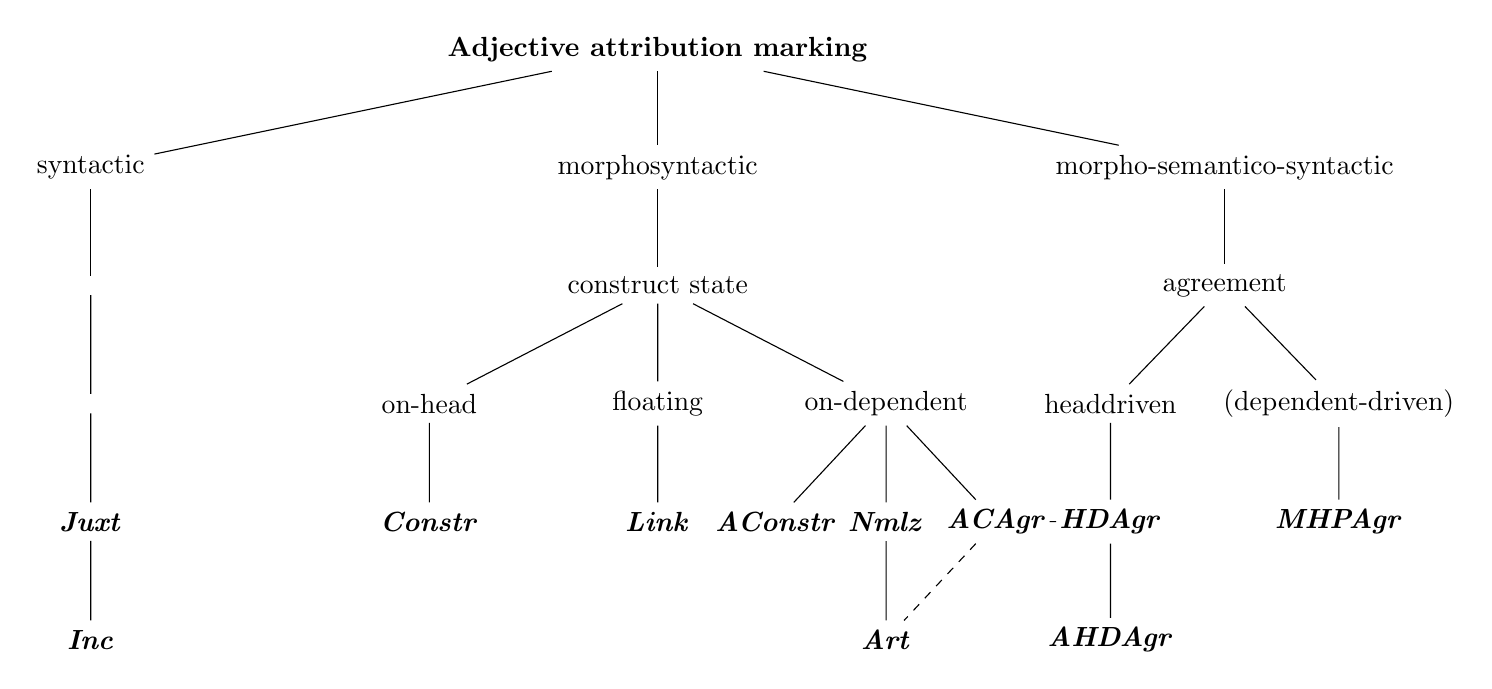
\begin{tikzpicture}
\tikzstyle{level 1}=[sibling distance=72mm]
\tikzstyle{level 3}=[sibling distance=29mm]
\tikzstyle{level 4}=[sibling distance=14mm]
\node {\textbf{Adjective attribution marking}}
child {node {syntactic}
	child {node {}
		child {node {}
			child {node {\textbf{\textit{Juxt}}}
				child {node {\textbf{\textit{Inc}}}
				}
			}
		}
	}
}
child {node {morphosyntactic}
	child {node {construct state}
		child {node {on-head}
			child{node {\textbf{\textit{Constr}}}
			}
		}
		child {node {floating}
			child{node {\textbf{\textit{Link}}}
			}
		}
		child {node {on-dependent}
			child{node {\textbf{\textit{AConstr}}}
			}
			child{node {\textbf{\textit{Nmlz}}}
				child{node (Art) {\textbf{\textit{Art}}}
				}
			}
			child{node (ACAgr) {\textbf{\textit{ACAgr}}}
			}
		}
	}
}
child {node {morpho-semantico-syntactic}
	child {node {agreement}
		child {node {head\hyp{}driven}
			child {node (HDAgr) {\textbf{\textit{HDAgr}}}
				child {node {\textbf{\textit{AHDAgr}}}
				}
			}
		}
		child {node {(dependent-driven)}
			child {node {\textbf{\textit{MHPAgr}}}
			}
		}
	}
};
\draw [dashed] (HDAgr) -- (ACAgr) -- (Art);
\end{tikzpicture}
\caption[Ontology of adjective attribution marking types]{Ontological tree of attested adjective attribution marking devices; type abbreviations are: ACAgr=Anti-construct state agreement, AConstr=Anti-construct state, AHDAgr=Appositive head\hyp{}driven agreement, Art=Attributive article, Constr=Construct state, HDAgr=Head\hyp{}driven agreement, Inc=Incorporation, Juxt=Juxtaposition, Link=Linker, MHPAgr=Modifier-headed possessor agreement, Nmlz=Attributive nominalization} 
\label{tree ontology}\bigskip
\end{sidewaysfigure}
\todo{LATEX: I need a solid line in the left branch of the tree}

%\documentclass{LSP/langsci}
%
%\usepackage{localmetadata}
%\usepackage{localpackages}
%\usepackage{localhyphenation}
%\usepackage{localcommands}
%\usepackage{authorindex}
%\bibliography{localbibliography}

%\begin{document}

\chapter[Polyfunctionality]{Excursus: Polyfunctionality of attribution marking devices} \label{polyfunctionality}
%%%
In a typological survey, noun phrases with adjectival modifiers can be examined from different perspectives. In the previous chapter, noun phrases with attributive adjectives were described according to their syntactic, morpho-syntactic, and/or morpho-semantico-syntactic structure. But noun phrase types of a given language can also be defined on a polyfunctionality scale with regard to the class of attributed elements beyond adjective attribution: Attributive adjectives and other adnominal modifiers (such as demonstratives, possessor nouns, adpositional phrases, clauses, etc.) may or may not be used in similar noun phrase structures.

Moreover, polyfunctionality is also relevant in languages where one and the same device is used as a nominal modification marker beyond attribution: for modification inside an adjective phrase (licensing, for instance, a degree word as modifier of an adjective) or as a modification marker inside an adpositional phrase (licensing, for instance, an adposition as determined by a noun phrase). \textit{Attribution marker} should thus be understood as a term denoting a subset of \textit{modification markers} relevant to nominal phrase structure in general.

Finally, the polyfunctionality concerns even the semantic content (or function) of certain devices beyond modification marking. 

In the present chapter, polyfunctionality of adjective attribution marking devices will be illustrated with examples from a few languages.

\section{Polyfunctionality of modification markers}
%%%
\todo{check zu possessor compounding Dahl 2004. The growth and maintenance of linguistic complexity. Studies in language companion series, 71. Amsterdam: John Benjamins.}
In many languages, more than one class of attributes belong to one and the same noun phrase type. Some languages exhibit even highly polyfunctional noun phrase types and use one and the same device for licensing verbs, nouns, adjectives and even other syntactic classes as attributive modifiers inside noun phrases.

In example (\ref{multi mand}) from Mandarin Chinese, the anti-construct state marker \textit{de} illustrates a highly polyfunctional attribution marking device. It licenses adjectival (\ref{mandarin adj}), nominal (\ref{mandarin noun}) and verbal attributes (\ref{mandarin rel}).\footnote{Note, however, that the attributive marker is not obligatory. In noun phrases with pronominal and adjectival attributes, it can also be omitted. If \textit{de} is used with adjectives, a certain clarifying or delineating stress is put on the denoted property, e.g.~\textit{hóng hūa} [red flower] ‘a red flower’, \textit{hóng de hūa} [RED \textsc{attr} flower] ‘a flower that is red (and not of a different color)’ \citep[119–123]{li-etal1981}.}
%%%
\begin{exe}
\ex
\langinfo{Mandarin Chinese}{Sinotibetan}{\citealt{li-etal1981}} \label{multi mand}
\begin{xlist}
\ex	\textrm{Noun (possessor) attribute}\\
\gll	Zhāngsān 	\textbf{de} 	shū\\
	Zhangsang 	{\textsc{attr}} 	book\\
\glt	‘Zhangsang's book’\label{mandarin noun}
\ex	\textrm{Adjectival attribute}\\
\gll	xīn 		(\textbf{de}) 	shū\\
	new	 	({\textsc{attr}}) 	book\\
\glt	‘new book’\label{mandarin adj}
\ex	\textrm{Verbal (relative clause) attribute}\\
\gll	wŏ zuótiān 	măi 	\textbf{de} 	shū\\
	1\textsc{1sg} 	buy	yesterday 	{\textsc{attr}} 	book\\
\glt	‘the book I bought yesterday’\label{mandarin rel}
\end{xlist}
\end{exe}
%%%
In Minangkabau, an Austronesian language spoken on Sumatra in Indonesia, juxtaposition is polyfunctional to a similar degree.
%%%
\begin{exe}
\ex 
\langinfo{Minangkabau}{Austronesian}{\citealt[3–4]{gil2005}} \label{multi minangkabau}
\begin{xlist}
\ex \textrm{Noun (possessor) attribute}\\
\gll	batiak Kairil\\
	papaya Kairil\\
\glt	‘Kairil's papaya’
\ex \textrm{Adjectival attribute}\\
\gll	batiak kuniang\\
	papaya yellow\\
\glt	‘a/the yellow papaya’
\ex \textrm{Verbal (relative clause) attribute}\\
\gll	batiak Kairil bali\\
	papaya Kairil buy\\
\glt	‘a/the papaya that Kairil bought’
\end{xlist}
\end{exe}
%%%
Tagalog is another language with a polyfunctional attribution marker. The Tagalog linker, however, is less polyfunctional than juxtaposition in Minangkabau or anti-construct state marking in Mandarin Chinese. It marks only verbal and adjectival attributes.\footnote{Note that that the constituent order of attribute and head noun is free in Tagalog: The relative clause and the adjective can also occur in a head-initial phrase type. In this case, the linker \textit{=ng} attaches phonologically to the noun (\citealt[1]{gil2005}; \citealt[160, 162]{himmelmann1997}).}
%%%
\begin{exe}
\ex 
\langinfo{Tagalog}{Austronesian}{\citealt[6]{gil2005}} \label{multi tagalog}
\begin{xlist}
\ex \textrm{Adjectival attribute}\\
\gll	pula\textbf{=ng} mangga\\
	red{=\textsc{attr}} mango\\
\glt	‘red mango’
\ex \textrm{Verbal (relative clause) attribute}\\
\gll	binili ni Jojo\textbf{=ng} mangga\\
	bought \textsc{pers.gen} Jojo{=\textsc{attr}} mango\\
\glt	‘mango that Jojo bought’
\end{xlist}
\end{exe}
%%%
Highly polyfunctional attribution marking by means of a head-marking construct suffix is found even in Persian.\footnote{Note the consistent glossing \textsc{mod} instead of \textsc{attr}. The Persian construct marker licenses modification beyond attribution.}
%%%
\begin{exe}
\ex 
\langinfo{Persian}{Indoeuropean}{\citealt{mahootian1997}}\label{multi persian}
\begin{xlist}
\ex \textrm{Modification inside an adpositional phrase}\\
\gll	tu\textbf{-ye} ašpæzxune\\
	in\textbf{-\textsc{mod}} kitchen\\
\glt ‘in the kitchen’
\ex \textrm{Nominal attribution}
\begin{xlist}
\ex \textrm{Noun (non-possessor) attribute}\\
\gll 	ængoštær\textbf{-e} ælmas\\
	ring-\textsc{mod} diamond\\
\glt 	‘diamond ring’
\ex \textrm{Noun (possessor) attribute}\\
\gll	ængoštær\textbf{-e} pedær\\
	ring-\textsc{mod} father\\
\glt	‘father's ring’
\end{xlist}
\ex \textrm{Adjectival attribute}\\
\gll	ælmas\textbf{-e} bozorg\\
	diamond-\textsc{mod} big\\
\glt	‘a big diamond’
\ex \textrm{Adpositional attribute}\\
\gll	miz\textbf{-e} tu{-ye} ašpæzxune\\
	table-\textsc{mod} in{-\textsc{mod}} kitchen\\
\glt ‘the table in the kitchen’
\ex \textrm{(Infinite) verbal attribute}\\
\gll	væqt\textbf{-e} ræftæn\\
	time-\textsc{mod} to\_go\\
\glt	‘time to go’
\end{xlist}
\end{exe}
%%%
While nominal, adjectival, adpositional and (infinite) verbal attributes are marked by the same device, finite verbal attributes (relative clauses) never occur in a similar noun phrase type in Persian.

In Västerbotten-Swedish, a language of the northern Eurasian area under investigation, attribution marking by means of adjective incorporation is also considered to be polyfunctional (cf.~Sections \ref{attr incorporation} and \ref{bondska synchr}). Beside adjective attribution, the device marks attribution of (human) possessors.
%%%
\begin{exe}
\ex 
\langinfo{Västerbotten-Swedish}{Indoeuropean}{\citealt[5]{gil2005}} \label{multi bondska}
\begin{xlist}
\ex \textrm{Noun (human possessor) attribute}\\
\gll	Pelle-äpple\\
	Pelle-apple\\
\glt	‘Pelle's apple’
\ex \textrm{Adjectival attribute}\\
%\begin{xlist}
%\ex (lexical adjective)
\gll	rö-äpple\\
	red-apple\\
\glt	‘red apple’
%\ex (past participle)
%\gll	(stick-ad)-tröja\\
%	(knitt-\textsc{ptcp:pst})-sweater\\
%\glt	‘knitted sweater’
%\end{xlist}
\end{xlist}
\end{exe}
%%%
\todo{bessere Referenz zu VB-Schwedisch??}
Gil (\citeyear{gil2005}) surveyed the polyfunctionality of attribution markers licensing possessor nouns, adjectives and relative clauses in a world-wide sample of languages. According to the number of morpho-syntactically differentiated classes of attributes Gil grouped the languages of his sample into the following types:
%%%
\begin{itemize}
\item \textbf{Weakly differentiating languages} using polyfunctional devices for attribution of all three syntactic categories, as in Mandarin (\ref{multi mand}) and Minangkabau (\ref{multi minangkabau})
\item \textbf{Moderately differentiating languages} using polyfunctional devices for attribution of two syntactic categories, for instance:
	\begin{itemize}
	\item adjectives and relative clauses, as in Tagalog (\ref{multi tagalog})
	\item possessor nouns and adjectives, as in Västerbotten-Swedish (\ref{multi bondska}) and Persian (\ref{multi persian})
	\end{itemize}
\item \textbf{Highly differentiating languages} are not polyfunctional at all, as in German where the three syntactic classes are marked differently.
\end{itemize}
%%%
In Gil's sample, Europe and adjacent parts of Asia and Africa stand out as an area with predominantly non-polyfunctional languages, while almost all languages of Southeast Asia are of low differentiation \citep[8]{gil2005}.

Northern Eurasian languages of the “moderately differentiating” type included in Gil's sample are Japanese and Västerbotten-Swedish (with polyfunctional attribution marking of possessor nouns and adjectives) as well as Ainu, Nivkh and Tatar (with polyfunctional attribution marking of adjectives and relative clauses).\footnote{Note that English is not coded as “moderately differentiating” by \citet{gil2005}, although juxtaposition can be polyfunctionally used as a device for attribution of adjectives and relative clauses (with reverse constituent order though: \textit{The woman I saw.})} No languages of the “weakly differentiated” type are known to occur in the northern Eurasian area. 
%%%
\begin{figure} \label{multi abcd}
\parbox[b]{0.20\textwidth}{
\begin{center}\textsc{Mandarin},\\\textsc{Minangkabau}\\
\medskip
\begin{tabular}{| l |}
\hline
\\
\hline
\hline
\\
\hline
\textsc{attr}$_{Rel}$\\
\hline
\textsc{attr}$_{A}$\\
\hline
\textsc{attr}$_{N}$\\
\hline
\end{tabular}
\end{center}
}
\parbox[b]{0.20\textwidth}{
\begin{center}\textsc{Tagalog}\\
\bigskip
\begin{tabular}{| l |}
\hline
\\
\hline
\hline
\\
\hline
\textsc{attr}$_{Rel}$\\
\hline
\textsc{attr}$_{A}$\\
\hline
\\
\hline
\end{tabular}
\end{center}
}
\parbox[b]{0.20\textwidth}{
\begin{center}\textsc{Västerbotten-}\\\textsc{Swedish}\\
\medskip
\begin{tabular}{| l |}
\hline
\\
\hline
\hline
\\
\hline
\\
\hline
\textsc{attr}$_{A}$\\
\hline
\textsc{attr}$_{N}$\\
\hline
\end{tabular}
\end{center}
}
\parbox[b]{0.20\textwidth}{
\begin{center}\textsc{Persian}\\
\bigskip
\begin{tabular}{| l |}
\hline
\textsc{mod}$_{NP}$\\
\hline
\hline
\textsc{attr}$_{AdP}$\\
\hline
\\
\hline
\textsc{attr}$_{A}$\\
\hline
\textsc{attr}$_{N}$\\
\hline
\end{tabular}
\end{center}
}
\caption[Functional map for modification marking]{Functional maps for modification markers: the anti-construct state marking in \textsc{Mandarin Chinese} and juxtaposition in \textsc{Minangkabau}, the linker in \textsc{Tagalog}, adjective incorporation in \textsc{Västerbotten-Swedish} and construct state marking in \textsc{Persian}}
\end{figure}
%%%
\figref{multi abcd} illustrates the polyfunctionality of modification markers in the languages mentioned in this chapter.\footnote{Cf.~\cite{haspelmath2003}, for a systematic and historiographic description of functional (or semantic) maps.} The true attributive functions of the marker, i.e.~licensing of adpositional, verbal, and adjectival attributes, are found in the middle cells of the left column in \figref{multi abcd}. The cell extending upwards shows the additional function of the marker as licensee of modification above the noun phrase level (i.e.~inside an adposition phrase).% or below the noun phrase level (i.e.~inside an adjective phrase).

The order of \textsc{attr}$_{Rel}$ through \textsc{attr}$_{N}$ in these functional maps corresponds to the hierarchical alignment of polyfunctional attribution marking suggested by Bingfu Lu and Zhenglin Qu.\footnote{Lu's and Qu's hierarchy, cited from a LingTyp posting (“The alignment of modification coding”, LingTyp Item \#2580, 6 May 2009, 01:36, \url{http://listserv.linguistlist.org/cgi-bin/wa?A2=ind0905A&L=LINGTYP&P=R146}) is based on a similar hierarchy for Austronesian languages by Foley (\citeyear{foley1980}). Note that Foley's hierarchy is proposed to be cross-linguistically valid and even includes two more syntactic classes than considered here: Determiner > Numeral > Noun > Adjective > Verb.}
\todo{gibt es eine Publikation inzwischen?}
%%%
\begin{exe}
\ex	Noun < Adjective < Verb
\end{exe}
%%%
The hierarchy is to be read as follows: The highest category of attributive modifiers are verbs (i.e.~relative and other attributive clauses), the next lower categories are adjectives and nouns. If one attributive category is marked with a polyfunctional attribution marker, the less bounded category adjacent to the left side in the hierarchy should be marked by the same device, too.
%%%
\begin{figure}
\parbox[b]{\textwidth}{
\begin{center}
\begin{tabular}{| l || c | c |}
\cline{1-1}
\\
\hline
\textsc{attr}$_{Rel}$ & \textsc{nmlz} & \textsc{foc}\\
\hline
\textsc{attr}$_{A}$\\
\cline{1-1}
\textsc{attr}$_{N}$\\
\cline{1-1}
\end{tabular}
\end{center}
}
\caption[Functional map for modification marking]{Functional map for the modification marker \textit{ve} in \textsc{Lahu}}
\label{lahu funcmap}
\end{figure}

\section[Polyfunctionality and additional content]{Polyfunctionality of modification markers and additional content}
%%%
Polyfunctional modification marking devices with semantic content (or function) beyond attribution are also attested in several languages. Lahu is an example of a Southeast Asian language of the “weakly differentiating” type according to Gil's (\citeyear{gil2005}) classification. Syntactically similar to Mandarin Chinese, Lahu exhibits an anti-construct state marker \textit{ve} that licenses adjectival (\ref{lahu adj}), nominal (\ref{lahu noun}) and verbal attributes (\ref{lahu rel}). In addition, the marker \textit{ve} in Lahu is used as nominalizer (\ref{lahu compl}) and as focus marker (\ref{lahu focus}).\footnote{See \citealt{bickel1999} on the “Standard Sino-Tibetan Nominalization pattern” which in some languages include even additional content beyond attribution, nominalization and focus.}
%%%
\begin{exe}
\ex
\langinfo{Lahu}{Sinotibetan}{\citealt{matisoff1973}}
\begin{xlist}
\ex	\textrm{Attribution}
\begin{xlist}
\ex	\textrm{Adjectival attribute}\\
\gll	dàʔ	\textbf{ve}	ŋâʔ\\
	pretty	\textsc{attr}	bird\\
\glt	‘pretty birds’ (194)\label{lahu adj}
\ex	\textrm{Noun (possessor) attribute}\\
\gll	Càl\^{ɔ}	\textbf{ve}	\`{ɔ}ha\\
	Jalaw	\textsc{attr}	picture\\
\glt	‘Jalaw's picture’ (141)\label{lahu noun}
\ex	\textrm{Verbal (relative clause) attribute}\\
\gll	c\'{ɔ}	câ	\textbf{ve}	ŋâʔ\\
	boil	eat	\textsc{attr}	bird\\
\glt	‘birds one boils to eat’ (194)\label{lahu rel}
\end{xlist}
\ex	\textrm{Additional semantic content}
\begin{xlist}
\ex \textrm{Nominalization (of a complement clause)}\\
\gll	n\`{ɔ}	qôʔ \textbf{ve}	thàʔ	ŋà mâ	na ɣa	qôʔ-ma!\\
	you	say \textsc{nmlz}	\textsc{acc} I	\textsc{neg} understand	be\_able	\textsc{interj}\\
\glt	‘I can't catch what you're saying!’ (157)\label{lahu compl}
\ex	\textrm{Focusing (of a clause)}\\
\gll	mâ		qay	\textbf{ve}\\
	\textsc{neg}	go	\textsc{foc}\\
\glt	‘I am certainly not going.’ (362)\label{lahu focus}
\end{xlist}
\end{xlist}
\end{exe}
%%%
The functions of the marker \textit{ve} in Lahu can also be summarized in a functional map, see \figref{lahu funcmap}. The true attributive functions of the marker, i.e.~licensing of verbal, nominal and adjectival attributes, are found in the cells of the left column in \figref{lahu funcmap}. The cells extending to the right show the additional content of the attributive marker, i.e.~as a nominalizer and focus marker of a clause.

\section{Conclusion}
%%%
From a purely synchronic point of view, polyfunctionality of adjective attribution marking devices seems less relevant to the area under investigation, northern Eurasia. Most languages of the area exhibit highly differentiated attribution marking devices. Languages of the “moderately differentiating” type are rare; no languages of the “weakly differentiated” type are known to occur in the northern Eurasian area at all.

However, polyfunctionality can perhaps indicate historical change if additional semantic content of attribution marking devices across related languages is taken into consideration. The topic of polyfunctional attribution markers across languages of one family will thus be taken up again in Part~\ref{part synchr} of this study.

%%%
\part{Synchrony} \label{part synchr} %
\part{Synchrony} \label{part synchr}


\chapter{Introduction}
%%%
The geographic area covered in the present survey stretches from Europe (including the Mediterranean Islands Malta and Cyprus as well as the regions Anatolia and the Caucasus\is{Caucasus}), over central,\is{Inner Asia} northern,\is{North Asia} and northeastern Asia\is{Northeast Asia} (including the whole of \isi{Siberia}, the adjacent parts of northern Mongolia) to the Islands of the northwestern Pacific Ocean. The language families represented in this area are genealogically categorized by \citet{salminen2007} in his chapter on the endangered languages of “\isi{Europe} and \isi{North Asia}”. By and large, Salminen's inventory of languages will be followed here. However, the present survey strictly follows the geography of northern Eurasia and consequently also includes Siberian Yupik Eskimo,\il{Siberian Yupik Eskimo} Ainu,\il{Ainu} the Sino-Tibetan language Dungan,\il{Dungan} and some Semitic\il{Semitic languages} languages.

\section{The languages of northern Eurasia}
%%%
Adopting Salminen's rather cautious genealogical classification the following families and isolates are considered (roughly from Northeast to Southwest):
%%%
\begin{multicols}{2}
\begin{enumerate}
\item{Eskimo-Aleut}\il{Eskimo-Aleut languages}
\item{Chukotko-Kamchatkan}\il{Chukotko-Kamchatkan languages}\footnote{Salminen describes Chukotkan\il{Chukotkan languages} and Kamchatkan\il{Kamchatkan languages} as two separate language families.}
\item{Nivkh}\il{Nivkh}
\item{Ainu}\il{Ainu}
\item{Japanese}\il{Japanese}
\item{Korean}\il{Korean}
\item{Sino-Tibetan}\il{Sino-Tibetan languages}
\item{Mongolic}\il{Mongolic languages}
\item{Tungusic}\il{Tungusic languages}
\item{Yukaghir}\il{Yukaghir languages}
\item{Yeniseian}\il{Yeniseian languages}
\item{Turkic}\il{Turkic languages}
\item{Nakh-Daghestanian}\il{Nakh-Daghestanian languages}
\item{Abkhaz-Adyghe}\il{Abkhaz-Adyghe languages}
\item{Kartvelian}\il{Kartvelian languages}
\item{Semitic}\il{Semitic languages}
\item{Uralic}\il{Uralic languages}
\item{Indo-European}\il{Indo-European languages}
\item{Basque}\il{Basque}
\end{enumerate}
\end{multicols}
%%%

Even though some of these genealogical units have been assumed to combine to larger stocks (such as Altaic,\il{Altaic languages} North Caucasian\il{North Caucasian languages} and others) the restriction to completely uncontroversial units seems adequate for the present areal typological investigation. This is especially true since an attempt is made to map variation inside genealogical units rather than to evaluate a statistically balanced genealogical sample of languages.

%Andreas Hölzl
%Nikh has several mutually unintelligible "dialects"
%Japanese is better called Japanese-Ryukyuan (or maybe Japonic) as there are at least two main branches of which Japanese is only one; Japanese itself has enough variation to consider it a small language family (e.g., Hachijo); Ryukyuan accordig to one view has the following complex structure: 1 Northern, 1.1 Amami (e.g. Okinoerabu), 1.2 Okinawan (e.g., Shuri), 2 Southern, 2.1 Miyako (e.g. Ogami), 2.2 Macro-Yaeyama, 2.2.1 Yaeyama (e.g. Hateruma), 2.2.2 Yonaguni (e.g. Dunan)
%there are many Mandarin dialects that are spoken at least as far north as Dungan (e.g. Northeast China, Xinjiang) and should thus be included
%the classification of Tungusic given below is somewhat outdated, today most scholars agree in two main branches and four subbranches. in the terminology of Janhunen (2012), these are: 1 Northern Tungusic, 1.1 Ewenic (e.g. Evenki), 1.2 Udegheic (e.g. Udihe), 2 Southern Tungusic, 2.1 Nanaic (e.g. Nanai), 2.2 Jurchenic (e.g. Manchu)
%perhaps better called Yukaghiric as there are still two rather different languages
%Maltese is located as far south as is Amdo Tibetan, Mandarin, Korean, and Japanese
%in Northeast Asia there are several mixed languages and Pidgins that are not easily classified here: Govorka, Chinese Pidgin Russian, Ejnu, Mednyj Aleut

Tungusic is also spoken in northern Siberia (Even, Evenki, formerly Arman) but there are almost no speakers in Mongolia

\section{The language sample}
%%%
All attested adjective attribution marking devices of languages mentioned in the present study are coded in a table in the Appendix.\footnote{The table is derived from \citet{AUTOTYP-NP} where these languages are coded for noun phrase patterns.} This table thus includes a relatively complete list of languages from the northern Eurasian area. At least one representative of each existing taxon is found in that sample. Additionally, several languages from within or outside the area (all of which are mentioned in other chapters of this investigation) or even other languages on which information was easily accessible are coded.

All languages are sorted alphabetically according to their genealogical affiliation. For each of the languages, the attested noun phrase type(s) relevant to adjective attribution marking are listed.

\section{The language maps}
%%%
The language maps have been generated using the data coded in the language sample in the Appendix.

\subsection[Geographic coding]{Data points for geographic coding}
%%%
Each language is displayed as one data point. The corresponding geographic coordinates have either been taken from \citet{walsOnline2013}\is{WALS} or were included using the language coordinates provided by \citet{AUTOTYP}.\is{AUTOTYP} For some languages, which were missing in the mentioned databases, new coordinates had to be defined based on the main geographic location where the respective languages are spoken.

Displaying the distribution of a given feature by means of a borderline around a group of languages~– like in the maps used by typological surveys of the EUROTYP\hyp{}project\footnote{\url{http://www.degruyter.com/view/serial/16329} (Accessed 2016-07-19)}~– was not preferred because these maps might imply the existence of isoglosses around continuous language and dialect areas. A typological survey of non-continuos languages seems rather inadequate for drawing such isoglosses.\footnote{Cf.~also Van Pottelberge's \citeyear{van-pottelberge2001} critique of the “name maps” used by EUROTYP. Furthermore, the EUROTYP language sample is somewhat arbitrary. The western Romance\il{West Romance languages} varieties, for instance, are represented in large number whereas varieties of Balkan Romance\il{Balkan Romance languages} (Megleno-Romanian,\il{Megleno-Romanian} Aromunian,\il{Aromunian} etc.) are missing completely. Also the whole Saamic\il{Saamic languages} branch is represented in the \isi{EUROTYP} sample as one single language only even though Saamic\il{Saamic languages} languages are as diverse as Romance\il{Romance languages} languages.}

\subsection[Type coding]{Data points for type coding}
%%%
In several languages more than one default attribution marking device occurs, for example in \ili{Albanian} (see \S\ref{albanian synchr}) where two lexical classes of adjectives exist: one of them marked for \isi{head\hyp{}driven agreement}, the other simultaneously marked for \isi{head\hyp{}driven agreement} and \isi{attributive nominalization}. In the map's legend, a slash marks the occurrence of multiple basic types in one language: \ili{Albanian} \textit{HDrAgr/Nmlz+HDrAgr}.\footnote{Type abbreviations are explained in the Appendix.}

Parentheses denote secondary types of attribution marking devices with additional semantic content, as in \ili{Chuvash} (see \S\ref{chuvash synchr}), where attributive adjectives are normally juxtaposed but can alternatively be marked for \isi{attributive nominalization} in contrastive focus constructions: \textsc{Chuvash}\il{Chuvash} \textit{Juxt(Nmlz)}.

Square brackets are used for languages where the occurrence of a given type of attribution marking device seems even more restricted or if the device's characteristics remain uncertain due to inadequate data. Consider for example \ili{Turkish} (see \S\ref{turkish synchr}), where \isi{attributive nominalization} occurs as a secondary type but is restricted to \isi{headless noun phrase}s in direct object position (marked for accusative): \textsc{Turkish}\il{Turkish} \textit{Juxt[Nmlz]}. 
Secondary and tertiary types are not coded in the maps. 

\subsection{The maps}
%%%
The maps in Figure~\ref{WorldMap} and Figure~\ref{WorldMapTyp} show the distribution of different adjective attribution marking devices across those world's languages mentioned in the present study. Whereas all types are coded with different colors or shapes in Figure~\ref{WorldMap}, a similar language sample is coded only for the main morpho-syntactic types (\isi{juxtaposition}, agreement, attributive state, \isi{incorporation}) in Figure~\ref{WorldMapTyp}. Note that these world maps do not reflect systematic sampling but are rather the result of random choice due to my work with data coded for the noun phrase structure module of \isi{AUTOTYP} \citep{AUTOTYP-NP}. Note also that the maps show fewer languages from the northern Eurasian area than are actually coded in the language sample in the Appendix.

The other pairs of maps are coded similarly but zoom in on northern Eurasia (Figure~\ref{NEMap} and Figure~\ref{NEMapTyp}), on \isi{North Asia} (Figure~\ref{NAMap} and Figure~\ref{NAMapTyp}) and on Europe (Figure~\ref{EUMap} and Figure~\ref{EUMapTyp}). Whereas the maps of northern Eurasia and \isi{North Asia} show only representatives for the known single taxa, the maps of Europe present a more complete picture. The reason for displaying a deeper resolution in the European map is the easier accessibility of data for almost all existing languages of that area. Displaying a similar deep resolution on the whole northern Eurasian area was not possible due to lack of data for several languages.

In order to present a balanced picture, several European languages are thus not displayed in the larger map of northern Eurasia. When a choice had to be made whether or not to keep a language inside a given taxon, this was always done in favor of diversity rather than uniformity. One taxon can even be represented by more than one language in order to display extraordinary diversity inside that group of closely related languages. Consequently, the northern branch of Germanic\il{North Germanic languages} is represented by Icelandic\il{Icelandic} (with \textit{HDrAgr}), Swedish\il{Swedish} (with \textit{ACAgr+HDrAgr/HDrAgr}) and Västerbotten Swedish\il{Swedish!Västerbotten} (with \textit{Inc/HDrAgr}) (\S\ref{n-germanic synchr}).

The choice to let the maps illustrate the highest possible diversity instead of displaying a genealogically and geographically balanced picture is justified by the general goal of the present investigation, namely the synchronic and diachronic mapping of cross-linguistically attested adjective attribution marking devices in a geographically restricted area. Whereas the mapping of synchronically attested diversity is the aim of the present part, Part~IV (Diachrony) will inspect this diversity form a diachronic perspective.

%sb index PARTLY
%===
%Haspelmath NO
%===
%example envir

\chapter[The languages of northern Eurasia]{Adjective attribution marking in the languages of northern Eurasia}
%%%

The following chapter contains an overall survey of adjective attribution marking devices which occur in the languages of northern Eurasia. For each genealogical unit, both the prototypical and the known minor noun phrase type(s) will be characterized and illustrated with examples. A complete list of adjective attribution marking devices in over 200 single languages considered for the present survey is found in Table~\ref{sample} starting on page \pageref{sample} in the appendix. The geographic spread of the different noun phrase types is shown on several Maps starting on page \pageref{WorldMap} in the appendix.

\il{Eskimo-Aleut languages|(}
\il{Eskimo languages|(}
\il{Yupik languages|(}
\il{Central Siberian Yupik|(}
\section{Eskimo-Aleut (Central Siberian Yupik)}
%%%
Whereas most languages of the Eskimo-Aleut family are spoken on islands in the Bering Strait or on the North American continent, a few varieties of the Yupik subbranch of Eskimo can be localized to north-easternmost Siberia. But only one of these languages, Central Siberian Yupik, is still spoken \cite[224]{salminen2007}.

In Central Siberian Yupik, only one adjective attribution marking device is attested:
%%%
\begin{itemize}
\item Incorporation.
\end{itemize}

\paragraph{Adjective incorporation in Central Siberian Yupik}
Property words (“adjectives”) in Central Siberian Yupik are phonologically bound nominal roots. Adjectival modification is thus expressed by means of polysynthetic morphology and can be characterized as adjective incorporation according to the ontology presented in Part~\ref{part typ}.
%%%
\begin{exe}
\ex \rm{Central Siberian Yupik \citep{de-reuse1994}}
\begin{xlist}
\ex
\gll	qawaagpag\textbf{-rukutaagh-\underline{gh}llag}-Ø\\
	legendary\_large\_bird-huge.\textsc{noun}-big.\textsc{noun}-\textsc{abs}\\
\glt	‘huge big (legendary large) bird’ (54)
\ex	
\gll	mangteghagh\textbf{-\underline{gh}llag}-lgu-uq\\
	house-big.\textsc{noun}-have.\textsc{noun}-\textsc{ind}(3s)\\
\glt	‘He has a large house.’ (55)
\ex	
\gll	mangteghagh\textbf{-\underline{gh}rugllag}-ngllagh-yug-nghit°e-unga\\
	house-big.\textsc{noun}-make.\textsc{noun}-want\_to.\textsc{verb}-\textsc{neg}-\textsc{ind(1s)}\\
\glt	‘I did not want to make a large house.’ (56)
\end{xlist}
\end{exe}
%%%
\il{Yupik languages|)}
\il{Central Siberian Yupik|)}
\il{Eskimo languages|)}
\il{Eskimo-Aleut languages|)}

\il{Chukotkan languages|(}
\section{Chukotkan}
%%%
The Chukotkan language family (aka Chukchi-Koryak)\il{Chukchi-Koryak|see{Chukotkan languages}} consists of two branches. The first branch, Chukchi, is represented by only one language, Chukchi, which has the same name as the branch itself. The second branch, Koryak-Alutor,\il{Koryak-Alutor languages} is represented by the two languages Alutor\il{Alutor} and Koryak\il{Koryak} proper. A third branch, Kerek,\il{Kerek languages} is probably extinct \cite[253]{salminen2007} and consequently not considered here.

Constituent order inside the noun phrase of Chukotkan languages is strictly head-final. Adjective attribution marking is also similar in all Chukotkan languages. Two types are attested:
%%%
\begin{itemize}
\item Incorporation
\item Head\slash{}driven agreement.
\end{itemize}

\il{Chukchi languages|(}
\subsection{Chukchi}
%%%
\paragraph{Adjective incorporation in Chukchi}
The use of the bound adjective morpheme in the polysynthetic structure (similar to Yupik)\il{Yupik languages} is illustrated in the following examples.\footnote{The vowel -ə- in these and the following examples is epenthetic.}
%%%
\begin{exe}
\ex \rm{Chukchi \citep{skorik1960}}
\begin{xlist}
\ex	
\gll	\textbf{elg-}ə-qoranə\\
	white-ə-deer:\textsc{abs.sg}\\
\glt	‘white reindeer’
\ex
\gll	\textbf{elg-}ə-qorat\\
	white-ə-deer:\textsc{abs.pl}\\
\glt	‘white reindeer (pl)’
\end{xlist}
\end{exe}
\il{Chukchi languages|)}

\il{Koryak-Alutor languages|(}
\subsection{Koryak}
%%%
\paragraph{Adjective incorporation in Alutor}
Similar to Chukchi,\il{Chukchi} adjective incorporation is the default adjective attribution marking device in Alutor.
%%%
\begin{exe}
\ex \rm{Alutor \citep{nagayama2003}}
\begin{xlist}
\ex
\gll	\textbf{meŋ-}ə-rara-ŋa\\
	big-ə-house-\textsc{abs.sg}\\
\glt	‘large house’
\ex
\gll	\textbf{meŋ-}ə-rara-wwi\\
	big-ə-house-\textsc{abs.pl}\\
\glt	‘large houses’
\end{xlist}
\end{exe}
\il{Koryak-Alutor languages|)}

\il{Chukchi|(}\il{Alutor|(}
\paragraph{Head\slash{}driven agreement in Chukchi and Alutor}
Whereas adjective incorporation is the default and unmarked type of adjective attribution marking in Alutor and Chukchi, several descriptions of the Chukotkan languages mention that adjectives can also occur in an unbound form (for Alutor \citealt{nagayama2003}; for Chukchi \citealt[103–104, 421–429]{skorik1960}, \citealt[251]{comrie1981}). As unbound morphemes adjectives take the stative marker \textit{n-} as well as agreement markers for person, number and case.
%%%
\begin{exe}
\ex \label{chukchi alutor free adj}
\begin{xlist}
\ex \rm{Chukchi \citep{skorik1960}}
\begin{xlist}
\ex
\gll	\textbf{n-ilg-ə-qin-Ø} qoranə\\
	\textsc{stat}-white-ə-\textsc{3sg} deer:\textsc{abs.sg}\\
\glt	‘white reindeer’
\ex
\gll	\textbf{n-ilg-ə-qine-t} qorat\\
	\textsc{stat}-white-ə-3-\textsc{pl} deer:\textsc{abs.pl}\\
\glt	‘white reindeer (pl)’
\end{xlist}
\ex \rm{Alutor \citep{nagayama2003}}
\begin{xlist}
\ex
\gll	\textbf{n-ə-meŋ-ə-qin} rara-ŋa\\
	\textsc{stat}-ə-big-ə-\textsc{abs:3sg} house-\textsc{abs.sg}\\
\glt	‘large house’
\ex
\gll	\textbf{n-ə-meŋ-ə-laŋ} rara-wwi\\
	\textsc{stat}-ə-big-ə-\textsc{abs:3pl} house-\textsc{abs.pl}\\
\glt	‘large houses’
\end{xlist}
\end{xlist}
\end{exe}
%%%
The number/person/case-agreement suffixes of adjectives and the suffixes marking possessive inflection of nouns belong to one and the same paradigm. Consequently, one could also interpret the Alutor and Chukchi data as another instance of modifier-headed possessor agreement (as in \ili{Oroch}, described in \S~\ref{ModheadAgr}). If so, the examples in (\ref{chukchi alutor free adj}) should be translated literally as ‘reindeer's whiteness’, ‘house's bigness’. An analysis avoiding syntactic dependency reversal between noun and adjective \citep[cf.][]{malchukov2000}, however, is preferred here for two reasons: The first reason is the constituent order inside the noun phrase. The assumed head shift to a modifier-headed possessor agreement construction would violate the otherwise strictly head-final constituent order rule in Alutor and Chukchi. 

The other reason arguing against syntactic head shift between noun and adjective is that in order to use non-incorporating constructions as in the examples in (\ref{chukchi alutor free adj}) the adjective is first transformed into a stative verb\is{stative verb} by means of a verbalizing prefix (\textit{-n}, glossed as \textsc{stat} in example \ref{chukchi alutor free adj}).

The verbalizer together with the agreement affix is sometimes glossed as an adjectivizing circumfix (\textsc{adjz>-\dots-<adjz:agr}), for instance in Nagayama's (\citeyear{nagayama2003}) grammatical description of Alutor. The given noun phrase type should then perhaps be analyzed as attributive state marking (as in Russian,\il{Russian} see \S\S~\ref{anti-constr agr}, \ref{russian synchr}). Unlike in Russian, however, the same agreement marking as in attributive constructions shows up on predicates as well.
%%%
\begin{exe}
\ex \rm{Alutor \citep{nagayama2003}}
\begin{xlist}
\ex
\gll	{\bf n-ə-tur-}iɣəm\\
	\textbf{\textsc{stat}-ə-young-}\textsc{1sg}\\
\glt	‘I'm young’
\end{xlist}
\end{exe}
%%%
Consequently, an analysis of adjective attribution marking in Alutor and Chukchi as belonging to the state marking type is rejected.

The semantic difference between the two constructions, with adjective incorporation on the one hand hand and head\hyp{}driven agreement marking on the other hand, is not clear. Whereas adjective incorporation is often described as the main or even only possible type (for Chukchi cf.~\citealt[37, 101]{kampfe-etal1995}), \citet[288]{kibrik-etal2000} state that this type indicates the corresponding quality or property as referring to background information in Alutor.

The following example from Chukchi, on the other hand, indicates that the non-incorporated adjective is used in an emphasized construction. Sentence (\ref{chukchi free adj}) was elicited by Vladimir Nedjalkov\ia{Nedjalkov, Vladimir} \citep[cited as pc in][330]{rijkhoff2002} in order to find examples of multiple modifiers in one noun phrase, which seems to be avoided by speakers of Chukchi. In sentence (\ref{chukchi inc adj}) with the incorporated adjective, the speaker simply left out the demonstrative when translating into Chukchi.
%%%
\begin{exe}
\ex \rm{Chukchi \citep[Vladimir Nedjalkov, pc, cit.][330]{rijkhoff2002}}
\begin{xlist}
\ex \label{chukchi free adj}
\gll	əngena-t ngəroq \textbf{n-ilg-ə-qine-t} qora-t\\
	this-\textsc{pl} three \textsc{stat}-white-ə-3-\textsc{pl} deer-\textsc{pl}\\
\glt	‘these three white reindeer’
\ex \label{chukchi inc adj}
\gll	ətlon ga-twetcha-twa-len ga-ngəron-\textbf{elg-}ə-qaa-ma\\
	\textsc{3sg} \textsc{pfct}-stand\_up-be-\textsc{3sg} \textsc{com}-white-ə-deer-\textsc{com}\\
\glt	‘He stood next to (these) three white reindeer.’
\end{xlist}
\end{exe}
%%%
\citet[716]{bogoras1922} states that the circum-positioned marker of the unbound adjective “sometimes corresponds to the definite\is{definiteness marking} article or designates an object as referred to before.” The unbound adjective, on the other hand, can only occur in absolutive case\is{case marking!absolutive} which is inherently connected to semantic definiteness\is{species marking!definite} \citep[cf.][207, elsewhere]{dunn1999}.
\il{Chukchi|)}
\il{Alutor|)}
\il{Chukotkan languages|)}

\il{Kamchatkan languages|(}
\il{Itelmen|(}
\section{Kamchatkan}
%%%
The only surviving member of the Kamchatkan language family is Itelmen (aka Western Kamchadal)\il{Western Kamchadal|see{Itelmen}} \citep[224]{salminen2007}.

The only attested type of adjective attribution marking in Itelmen is:\footnote{According to Volodin (\citeyear{volodin1997}) a few adjectives (among them Russian\il{Russian} loan adjectives) occur in juxtaposition.}
%%%
\begin{itemize}
\item Anti-construct state agreement.
\end{itemize}

\paragraph{Anti-construct state agreement in Itelmen} \label{itelmen synchr}
Constituent order inside the noun phrase of Itelmen is head-final. Adjectives form a class syntactically clearly distinguished from nouns: unlike the latter, adjectives are never represented by their root morphemes alone. Unlike verbs, which take TAM\is{TAM marking} markers, adjectives take adjectival morphology and are licensed either by an attributive or predicative\is{predicative marking} (adverbal) suffix (\citealt{volodin1997}, \citealt[54]{georg-etal1999}).
%%%
\begin{exe}
\ex \label{itelmen ex}
\rm{Itelmen \citep{volodin1997}} 
\begin{xlist}
\ex \rm{Attributive state of adjectives}\\
\gll	thun\textbf{-lah}\\
	dark-\textsc{attr}\\
\glt	‘dark’
\ex \rm{Predicative state of adjectives}\\
\is{predicative marking}
\gll	thun\textbf{-k}\\
	dark-\textsc{pred}\\
\glt	‘(is) dark’
\end{xlist}
\end{exe}
%%%
Since attributive adjectives also agree in case (though restricted to instrumental\is{case!instrumental} case), the noun phrase type can be characterized as anti-construct state agreement, structurally similar to the type found in Russian.\il{Russian} Consider the following example.\footnote{Note that the shape of the state marking suffix \textit{-lan'ļ} ($\leftarrow$ \textit{-lah-ļ}) is the result of a regular morpho-phonological process \citep{georg-etal1999}.}
%%%
\begin{exe}
\ex \rm{Anti-construct state agreement in Itelmen \citep{georg-etal1999}}\\
\gll	Kəmma çasit t'-nu-qz-al-kiçen \textbf{teŋ-lan'ļ} \textbf{thalthe-ļ}, min kn-anke t-zapasa-qzo-çen.\\
	\textsc{1sg} now \textsc{1sg}>-eat-\textsc{ipfv-fut-<1sg} good-\textsc{attr:ins} meat-\textsc{ins} \textsc{rel} \textsc{1sg-dat} \textsc{1sg}-keep-\textsc{ipfv-3sg-prtc}\\
\glt	‘Now I will eat the good meat which I kept for you.’
\end{exe}
\il{Itelmen|)}
\il{Kamchatkan languages|)}

\il{Nivkh|(}
\section{Nivkh}
%%%
Nivkh (aka Gilyak)\il{Gilyak|see {Nivkh}} is an isolated language spoken in the far east on the Eurasian continent on Sakhalin Island in easternmost Russia \citep[222–223]{salminen2007}.

The only type of adjective attribution marking attested in Nivkh is:
%%%
\begin{itemize}
\item Head\slash{}driven agreement.
\end{itemize}

\paragraph{Head\slash{}driven agreement in Nivkh}
Property words in Nivkh are verbal roots. As modifiers in noun phrases these adjectival verbs occur to the left of the head noun in a construction which is sometimes described as a polysynthetic structure (cf.~\citealt[16]{gruzdeva1998}; \citealt[80]{jakobson1971}, quoted by \citealt[138]{rijkhoff2002}). The reason for analyzing adjectives in Nivkh as being incorporated into the modified noun is the phonological boundedness of the constituents evidenced by regular alternations in the initial segments of the noun stem \cite[16]{gruzdeva1998}.
%%%
\begin{exe}
\ex \rm{Nivkh \citep[16]{gruzdeva1998}}
\begin{xlist}
\ex tu ‘lake’
\ex 
\gll	pily-du\\
	be\_big-lake\\
\glt	‘large lake’
\end{xlist}
\end{exe}
%%%
In her sketch grammar of Nivkh, however, \cite{gruzdeva1998} writes adjectival words consistently as morphologically unbound words.\footnote{For instance \textit{čuz pitɣy-Ø} [new book-\textsc{nom}] (19), \textit{kyla n'iɣvn̦} [high man] (33), \textit{pila eri} [big river] (38).}

Interestingly, the phonological stem alternation rules also apply to the plural inflection of nouns and their adjectival attributes by means of reduplication.\is{reduplication} Thus, in (\ref{nivkh redup}), the reduplicated stem of the participle \textit{t'osk̦} ‘destroyed’ is realized as \textit{-zosk̦}.
%%%
\begin{exe}
\ex \label{nivkh redup}
\rm{Nivkh (Ekaterina Gruzdeva, pc)}
\begin{xlist}
\ex 
\gll	tuin \textbf{t'osq-mu} hum-d'\\
	here break.\textsc{ptcp}-boat be-\textsc{ind}\\
\glt	‘there is a destroyed boat here’ 
\ex \label{nivkh unaltered}
\gll	tuin \textbf{t'osq\textasciitilde zosk̦-mu-ɣu} hum-d'[-ɣu]\\
	here break.\textsc{ptcp}\textasciitilde \textsc{pl}-boat-\textsc{pl} be-\textsc{ind}[-\textsc{pl}]\\
\glt	‘there are destroyed boats here’
\end{xlist}
\end{exe}
%%%
Note that the number agreement of the attributive forms of adjectives by means of reduplication is archaic. According to Ekaterina Gruzdeva (pc),\ia{Gruzdeva, Ekaterina} attributive adjectives practically never reduplicate\is{reduplication} any more. Examples of reduplicating adjectives are, however, included in the older grammar by Panfilov (\citeyear{panfilov1965}).
\il{Nivkh|)}

\il{Ainu|(}
\section{Ainu}
%%%
Ainu is an isolate spoken on Hokkaido Island in northern Japan.

The only type of adjective attribution marking attested in Ainu is:
%%%
\begin{itemize}
\item Juxtaposition.
\end{itemize}

\paragraph{Juxtaposition in Ainu}
\label{ainu synchr}
Ainu does not exhibit morphological differences between adjectives and verbs \citep[27]{refsing1986}. Words expressing states (\ref{ainu state}) or properties (\ref{aini qual}) in Ainu are best described as stative verbs.\is{stative verb} They form a subclass of intransitive verbs and are only semantically distinguished from verbs denoting an action \cite[141–142]{refsing1986}. As modifiers of a noun these property words are juxtaposed to the left.
%%%
\begin{exe}
\il{Ainu!Shizunai}
\ex \rm{Ainu (Shizunai) \citep[142]{refsing1986}}%!!CHECK PAGES
\begin{xlist}
\ex \rm{“State adjective”}\\ \label{ainu state}
\gll	\textbf{mokor} cep\\
	sleep fish\\
\glt	‘a sleeping fish’
\ex \rm{“Quality adjective”}\\ \label{aini qual}
\gll	\textbf{pirka} cep\\
	be\_good fish\\
\glt	‘a fine fish’
\end{xlist}
\end{exe}
\il{Ainu|)}

\il{Japanese|(}
\section{Japanese}
%%%
The noun phrase structure in Japanese, an isolated language, is strictly head-final. Two types of adjective attribution marking devices are attested:
\begin{itemize}
%%%
\item Juxtaposition
\item Anti-construct state marking.
\end{itemize}
%??\is{adjectivizer}
\paragraph{Juxtaposition in Japanese}
Two distinct lexical classes of words describe the state that an entity is in. Verbal adjectives belong to the first class. These adjectives are distinguished from stative verbs\is{stative verb} by the adjectivizer suffix \textit{-i}. Used as predicates, the adjectivized verbs marked with \textit{-i} follow the noun but do not require any copula. Attributive adjectives, on the other hand, are juxtaposed to the left of the modified noun. 
%%%
\todo{Martin: kono?}
\begin{exe}
\ex \rm{Verbal adjectives in Japanese \citep[170]{backhouse1984}}
\begin{xlist}
\ex \rm{Adjective predication}\\
\gll	kona rombun-wa \textbf{naga-i}\\
	this article-\textsc{top} long-\textsc{adjz}\\%check gloss ??PRES ??kono
\glt	‘This article is long.’
\ex \rm{Adjective attribution}\\
\gll	\textbf{naga-i} rombun\\
	long-\textsc{adjz} article\\
\glt	‘long article’
\end{xlist}
\end{exe}
%%%
Since the adjectivizer suffix \textit{-i} simply marks stative roots as (attributive and predicative) adjectives, it is not considered an attribution marking device. Hence, the class of verbal adjectives in Japanese is merely attributed by juxtaposition. Constituent order is crucial for differentiating attributive from predicative adjectives. 

\paragraph{Anti-construct state in Japanese}
Unlike “verbal adjectives”, which were described in the previous section, the few members of the second adjectival sub-class, i.e.~“nominal adjectives” require a special attributive form marked by the invariable attributive suffix \textit{-na}.
\todo{Martin: How do you say ‘the person is beautiful’? Isn't the -na just like the -i, somply an ADJ marker?}
%%%
\begin{exe}
\ex \rm{Japanese \citep[72–81]{pustet1989}}%!!REF stimmt nicht
\begin{xlist}
\ex \rm{Attribution: verbal adjective}\\
\gll	\textbf{waka-i} hito\\
	young-\textsc{adjz} person\\
\glt	‘a young person’
\ex \rm{Attribution: nominal adjective}\\
\gll	\textbf{kiree-na} hito\\
	beautiful-\textsc{attr} person\\
\glt	‘a beautiful person’
\end{xlist}
\end{exe}
%%%
Note that the word class boundary between nominal adjectives and nouns in Japanese is not always clear because some words take either the noun attribution marker \textit{-no} (\ref{japan na}) or the adjective attribution marker \textit{-na} (\ref{japan no}) when modifying a noun. The arbitrary behavior of attribution marking of nouns and nominal adjectives in Japanese indicates the continuous nature of these two word classes in this language \citep[79–80]{pustet1989}.
%%%
\begin{exe}
\ex \rm{Japanese \citep[72–81]{pustet1989}}%!!REF stimmt nicht
\begin{xlist}
\ex \rm{Noun attribution}\\ \label{japan na}
\gll	\textbf{wazuka-na} okane\\
	little-\textsc{attr} money\\
\glt	‘little money’
\ex \rm{Adjective attribution}\\ \label{japan no}
\gll	\textbf{wazuka-no} okane\\
	little-\textsc{attr} money\\
\glt	‘little money’
\end{xlist}
\end{exe}
\il{Japanese|)}

\il{Korean|(}
\section{Korean}
%%%
Korean is an isolated language spoken on the Korean peninsula in northeastern Asia. The only type of adjective attribution marking attested in Korean is:
%%%
\begin{itemize}
\item Anti-construct state marking.
\end{itemize}
%%%
Note, however, that Korean does not have a distinct class of adjectives but adjectival notions are expressed by verbs.

\paragraph{Anti-construct state in Korean}
The constituent order in the noun phrase of Korean is strictly head-final. Modifying “property words” are verbs equipped with a special attributive suffix \textit{-(u)n} \citep{martin-etal1969}.
%%%
\begin{exe}
\ex \rm{Korean \citep[61]{chang1996}}
\begin{xlist}
\ex
\begin{xlist}
\ex
\gll	i \textbf{ppalka-n} chayk\\
	this be\_red-\textsc{attr} book\\
\ex	
\gll	i \textbf{ppalka-n} chayk i\\
	this be\_red-\textsc{attr} book \textsc{subj}\\
\glt	‘this red book’
\end{xlist}
\ex
\begin{xlist}
\ex	
\gll	ce \textbf{khu-n} namwu\\
	that be\_big-\textsc{attr} tree\\
\ex
\gll	ce \textbf{khu-n} namwu lul\\
	that be\_big-\textsc{attr} tree \textsc{obj}\\
\glt	‘that big tree’
\end{xlist}
\end{xlist}
\end{exe}
\il{Korean|)}

\il{Sino-Tibetan languages|(}
\il{Dungan|(}
\section{Sino-Tibetan (Dungan)}\label{sinotibetan synchr}
%%%
The Sino-Tibetan language family is represented in northern Eurasia only by one language, Dungan (aka Dunganese),\il{Dunganese|see{Dungan}} which is a Gansu\il{Gansu languages} variety of Chinese spoken in the Kyrgyz Republic in \isi{Inner Asia} (cf.~\citealt[85]{yuo2003}, \citealt{kalimov1968}).

Two types of adjective attribution marking are attested in Dungan:
%%%
\begin{itemize}
\item Juxtaposition
\item Attributive nominalization.
\end{itemize}

\paragraph{Juxtaposition in Dungan}
Adjective attribution marking in the unmarked noun phrase in Dungan is characterized by juxtaposition. Hereby, the adjective either precedes or follows the noun.
%%%
\begin{exe}
\ex \rm{Dungan \citep[480]{kalimov1968}} \label{dungan juxtap}
\begin{xlist}
\ex 	
\gll	\textbf{da} fonzy\\
	big house\\
\ex
\gll	fonzy \textbf{da}\\
	house big\\
\glt	‘large house’
\end{xlist}
\end{exe}

\is{attributive nominalization|(}
\paragraph{Attributive nominalization in Dungan}
A second noun phrase type with the adjectival modifier marked by a suffix \textit{-di\textsuperscript{1}} occurs in Dungan as well. Whereas juxtaposition constitutes the general and unmarked type of adjective attribution marking, the attributive suffix \textit{-di\textsuperscript{1}} seems to be much more restricted and occurs for example in connection with a comparative (\ref{dungan compattr}) or negated attribute (\ref{dungan negattr}).
%%%
\todo{Martin: Sevaxina\\Micha:I use the German scientific transliteration}
\begin{exe}
\ex \rm{Dungan}
\begin{xlist}
\ex \rm{Negated attribute \citep[80]{zevachina2001}}\\
\label{dungan negattr}
\gll	gubuə\textsuperscript{3} bu\textsuperscript{1} \textbf{da\textsuperscript{3}-di\textsuperscript{1}} gun\textsuperscript{1}fu\textsuperscript{1}\\
	went \textsc{neg} big-\textsc{attr} time\\
\glt	‘Not much (lit. ‘not big’) time passed.’
\ex \rm{Comparative attribute \citep[480]{kalimov1968}}\\
\label{dungan compattr}
\gll	\textbf{da-ščer-di} fonzy\\
	bigger-\textsc{compar}-\textsc{attr} house\\
\glt	‘a somewhat larger (i.e.~different) house’\footnote{Note that the quoted transcriptions of the two authors differ from each other.}
\end{xlist}
\end{exe}	
%%%
The marker \textit{-di\textsuperscript{1}} is clearly cognate with the functionally similar nominalizer \textit{-de} in Mandarin Chinese\il{Mandarin Chinese} (cf.~Example \ref{multi mand} in \S~\ref{polyfunctionality}). In Dungan, however, \textit{-di\textsuperscript{1}} is sometimes also described as a marker of predicative\is{predicative marking} adjectives, as in (\ref{dungan emphpred}).
%%%
\begin{exe}
\ex \rm{Attributive nominalization in Dungan \citep[82]{zevachina2001}}\\
\label{dungan emphpred}
\gll	ž̨y\textsuperscript{3}gə\textsuperscript{1} mə\textsuperscript{1}mə\textsuperscript{2} \textbf{gan\textsuperscript{1}-di\textsuperscript{1}}\\
	this bread stale-\textsc{attr}\\
\glt	‘This bread is STALE (i.e.~different).’
\end{exe}
%%%
\citet[82]{zevachina2001} labels the function of the marker as an “emphasizing-predicative”. But looking at her other examples it becomes obvious that \textit{-di\textsuperscript{1}} does not mark predicative adjectives but rather nominalized attributive adjectives.
%%%
\begin{exe}
\ex \rm{Attributive nominalization in Dungan \citep[82]{zevachina2001}}\\
\gll	ž̨y\textsuperscript{3}gə\textsuperscript{1} fu\textsuperscript{1} bu\textsuperscript{1}cy\textsuperscript{1} \textbf{xun\textsuperscript{1}-di\textsuperscript{1}}, \textbf{zy\textsuperscript{2}-di\textsuperscript{1}}\\
	this book \textsc{neg} red-\textsc{attr} bordeaux-\textsc{attr}\\
\glt	‘This book is not RED, but BORDEAUX.’\\
	(lit. ‘This book is not a red one, but a bordeaux one.’)
\end{exe}
%%%
The nominalizing function of the suffix is also described by \cite{kalimov1968}.
%%%
\begin{exe}
\ex \rm{Attributive nominalization Dungan \citep[484]{kalimov1968}}\\ \label{dungan nmlz}
\gll	\textbf{ščin-di} gǔjdixyn\\
	new-\textsc{attr} expensive\\
\glt	‘The new (one) is expensive.’
\end{exe}
Attributive marking with the suffix \textit{-di\textsuperscript{1}} in Dungan needs to be investigated in more detail, especially in connection to constituent order. The head-initial structure seems to be used in order to emphasize the property denoted by the adjective.

However, according to the descriptions of Dungan taken into account here (i.e.~\citealt{kalimov1968} and \citealt{zevachina2001}), the language exhibits two adjective attribution marking devices: juxtaposition and attributive nominalization by means of the article \textit{-di\textsuperscript{1}}. While juxtaposition (with the order adjective-noun) seems to be the unmarked type, attributive nominalization is restricted to certain pragmatically\is{pragmatic marking} marked constructions.
\is{attributive nominalization|)}
\il{Dungan|)}
\il{Sino-Tibetan languages|)}

\il{Mongolic languages|(}
\section{Mongolic}
%Mongolic-nördliches China: Dagurisch, Mongorisch, Bao'an, Donxiang, Oirat
The Mongolic language family consists of five branches (cf.~\citealt[222]{salminen2007}): The core branch, Mongolian, includes the languages Kalmyk,\il{Kalmyk} Khalkha,\il{Khalkha} Khamnigan Mongol,\il{Khamnigan Mongol} and Oyrat\il{Oyrat} (aka Oirat).\il{Oirat|see{Oyrat}} Kalmyk is spoken in easternmost \isi{Europe} (in the Republic of Kalmykia of the Russian Federation). The other Mongolian languages are all spoken in \isi{Inner Asia}, along with Dagur\il{Dagur} which belongs to a satellite branch of the Mongolic family. Languages of the remaining three satellite branches of Mongolic are not considered here since they are all spoken outside the northern Eurasian area.

With regard to their principal noun phrase structure, all Mongolic languages of northern Eurasia exhibit the inherited \ili{Proto\hyp{}Mongolic} features, including strictly head-final constituent order and juxtaposition of attributive adjectives (“adjectival nouns”) as the only attribution marking device.

Note, however, that adjectives in Mongolic languages do not differ formally from regular nouns but are distinguishable from the latter only by their syntactic behavior and specific derivational patterns (cf.~\citealt[10]{janhunen2003b} for Proto\hyp{}Mongolic\il{Proto\hyp{}Mongolic} and \citealt[161]{svantesson2003} for Khalkha).\il{Khalkha}\footnote{In the two Mongolic languages \ili{Moghol} (spoken in Afghanistan) and Mangghuer\il{Mangghuer} (spoken in China) there is a distinct class of adjectives (cf.~\citealt[252]{weiers2003} for Moghol and \citealt[311]{slater2003} for Mangghuer). However, these languages are not considered since they are spoken outside the northern Eurasian area.}

The only type of adjective attribution marking attested in Mongolic languages of northern Eurasia is:
%%%
\begin{itemize}
\item Juxtaposition.
\end{itemize}

\il{Mongolian languages|(}
\subsection{Mongolian}
%%%
\paragraph{Juxtaposition in Khalkha}
The only attested adjective attribution marking device in the languages of the Mongolian branch of Mongolic is \textbf{juxtaposition}, similar to the following example. 
%%%
\begin{exe}
\ex \rm{Khalkha \citep{svantesson2003}}
\label{khalkha juxt}
\begin{xlist}
\ex
\gll	sayin nom\\
	good book\\
\glt	‘good book’
\ex 
\gll	sayin nom-uud\\
	good book-\textsc{pl}\\
\glt ‘good books’
\end{xlist}
\end{exe}
\il{Mongolian languages|)}

\il{Monguor languages|(}
\il{Moghol languages|(}
\il{Dagur languages|(}
\subsection{Monguor, Moghol, Dagur}
%%%
The only attested adjective attribution marking device in the languages of the Monguor, Moghol and Dagur branches of Mongolic is \textbf{juxtaposition} \citep{slater2003,weiers2003,tsumagari2003}, similar to example (\ref{khalkha juxt}) from Khalkha Mongolian.
\il{Monguor languages|)}
\il{Moghol languages|)}
\il{Dagur languages|)}
\il{Mongolic languages|)}

\il{Tungusic languages|(}
\section{Tungusic} \label{tungusic synchr}
%%%
The Tungusic language family (aka Manchu-Tungus)\il{Manchu-Tungus languages|see{Tungusic languages}} comprises several languages belonging to the three branches North Tungusic, Amur Tungusic and Manchu, all spoken in southern Siberia (Russia), northern Mongolia and northern China.

The constituent order inside the noun phrase in all Tungusic languages is relatively strictly head-final. In several Tungusic languages, attributive adjectives (“adjectival nouns”) are simply juxtaposed with the modified noun. This type is also mentioned as being prototypical of adjective attribution marking devices in Tungusic languages (e.g.~\citealt{sunik1968a}; \citealt[133]{kormusin2005}). However, several other types occur as well. The following adjective attribution marking devices are attested in Tungusic:
%%%
\begin{itemize}
\item Juxtaposition
\item Head\slash{}driven agreement
\item Attributive nominalization
\item Modifier-headed possessor agreement.
\end{itemize}

\il{North Tungusic languages|(}
\subsection{North Tungusic}
%%%
Languages belonging to the northern branch of Tungusic are Even (aka Lamut), Evenki (aka Oroqen in China), Negidal and Solon (aka Ewenke in China).

The major North Tungusic languages, Even and Evenki, deviate from the Tungusic prototype and exhibit head\hyp{}driven agreement as their general type (\citealt[11]{malchukov1995}; \citealt[18]{bulatova-etal1999}). Attributive nominalization and modifier-headed possessor agreement occur in these two languages as well, even though these devices are restricted to specially marked noun phrase types.

\il{Even|(}
\paragraph{Head\slash{}driven agreement in Even}
According to \citet[20]{malchukov1995}, the occurrence of head\hyp{}driven agreement marking of adjectives in Even is determined by discourse-pragmatic factors: Attributes in the rhematic (focus) position always agree with their heads, whereas agreement is optional in non-focus positions \cite[31–32]{malchukov1995}.\footnote{According to \cite[31]{malchukov1995}, regular head\hyp{}driven agreement occurs as the default type of adjective attribution marking only in literary Even and hence in prescriptive grammars. This does not reflect, however, the actual language use.}
%%%
\begin{exe}
\ex \label{even raising}
\rm{“Attribute raising agreement” in Even \cite[30–31]{malchukov1995}}
\begin{xlist}
\ex
\label{even juxt}
\rm{Juxtaposition}\\
\rm{(A N-\textsc{number}-\textsc{case})}\\
\gll	\textbf{Eŋi} beji-l-bu emu-re-m.\\
	strong man-\textsc{pl}-\textsc{acc} bring-\textsc{nonfut}-\textsc{1sg}\\

\ex
\label{even numagr}	
\rm{Incomplete head\hyp{}driven agreement}\\
\rm{(A-\textsc{number} N-\textsc{number}-\textsc{case})}\\
\gll	\textbf{Eŋi-l} beji-l-bu emu-re-m.\\
	strong-\textsc{pl} man-\textsc{pl}-\textsc{acc} bring-\textsc{nonfut}-\textsc{1sg}\\

\ex
\label{even agr}	
\rm{Complete head\hyp{}driven agreement}\\
\rm{(A-\textsc{number}-\textsc{case} N-\textsc{number}-\textsc{case})}\\
\gll	\textbf{Eŋi-l-bu} beji-l-bu emu-re-m.\\
	strong-\textsc{pl}-\textsc{acc} man-\textsc{pl}-\textsc{acc} bring-\textsc{nonfut}-\textsc{1sg}\\
\glt	‘I have brought back only strong men.’
\end{xlist}
\end{exe}
%%%
\citet[30–31]{malchukov1995} describes the attributive agreement patterns in Even in a hierarchical way: The adjective modifier can agree in all morphological features of the head-noun (\ref{even agr}) or just in number (\ref{even numagr}). Juxtaposition is also possible but restricted to adjectives in non-focus position (\ref{even juxt}).

\paragraph{Attributive nominalization in Even (I)}
The “attribute raising agreement” illustrated in the previous section (\S~\ref{even raising}) can be extended with a fourth step, specifically with adjective attributes marked by the “restrictive”\is{restrictive marking|see{definite marking}}\is{definite marking} marker \textit{=takan/=teken} (here glossed as a nominalizer).
%%%
\begin{exe}
\ex 
\rm{Even \citep[32]{malchukov1995}}
\begin{xlist}
\ex[]{ 
\gll	\textbf{Eŋi-l-bu=tken} beji-l-bu emu-re-m.\\
	strong-\textsc{pl}-\textsc{acc}=\textsc{nmlz} man-\textsc{pl}-\textsc{acc} bring-\textsc{nonfut}-\textsc{1sg}\\
	}
%%%
\ex[*]{	
\gll	\textbf{Eŋi=tken} beji-l-bu emu-re-m.\\
	strong=\textsc{nmlz} man-\textsc{pl}-\textsc{acc} bring-\textsc{nonfut}-\textsc{1sg}\\
\glt	‘I have brought back only strong men.’
}
\end{xlist}
\end{exe}
%%%
Attributes marked as “restrictive” obligatorily agree with the head noun \cite[32]{malchukov1995}. Noun phrases marked by means of \textit{=takan / =teken} thus resemble the attributive nominalization type, i.e.~the attribute is marked as a syntactically complex constituent (i.e.~as an embedded complement to the head noun) by means of nominalization.

\paragraph{Attributive nominalization in Even (II)}
A second attributive nominalization strategy by means of the possessive suffix 3\textsuperscript{rd} person singular (in “determinative”\is{definite marking} function; here glossed as a nominalizer) is attested in an investigation of the non-possessive use of the possessive marker in different Turkic and Tungusic languages \citep{benzing1993b}.
%%%
\begin{exe}
\ex 
\rm{Even \citep[17–18 Footnote 58]{benzing1993b}}\\
\gll	hagdiŋata\textbf{-n} orolcemŋā\\
	oldest-\textsc{nmlz} reindeer\_herder\\
\glt	‘the OLDEST reindeer herder’
\end{exe}
%%%
According to \cite[17–18 Footnote 58]{benzing1993b}, the “determinative”\is{definite marking} suffix {\it -n} ($\Leftarrow$ \textsc{poss:3sg}) can be used as a marker of contrastive focus in Even.
\il{Even|)}

\il{Evenki|(}
\paragraph{Modifier-headed possessor agreement in Evenki}
Evenki follows the general Tungusic rule of head-final constituent ordering inside the noun phrase. In constructions emphasizing the property denoted by the attributive adjectives, however, the unmarked adjective-noun order can be reversed. In these constructions, the adjective is obligatorily equipped with the possessive suffix 3\textsuperscript{rd} person (singular or plural).
%%%
\begin{exe}
\ex 
\rm{Evenki \citep[18]{bulatova-etal1999}}
\begin{xlist}
\ex	
\gll	\textbf{aja} bəjə\\
	good man\\
\glt	‘good man’
\ex \label{evenki poss}
\gll	bi: bəjə \textbf{aja-βa:-n} sa:-m\\
	\textsc{1sg} man good-\textsc{acc}-\textsc{poss:3sg} know-\textsc{1sg}\\
\glt	‘I know the GOOD man’
\end{xlist}
\end{exe}
%%%
According to \citet[18]{bulatova-etal1999}, the phrase final adjective ‘good’ marked with the possessive suffix is used as a true possessive noun in example (\ref{evenki poss}) and they translate the example like this: ‘I know the man's goodness’. This construction, however, is similar to the modifier-headed possessor agreement described for \ili{Oroch} (\ref{oroch modhead}) and Udege\il{Udege} (\citealt[485, elsewhere]{nikolaeva-etal2001}).\footnote{Similar modifier-headed constructions are found in Even where modifier-headed possessor agreement is in fact attested, cf.~\textit{Asatkan \textbf{nood-do-n} haaram.} [girl beautiful-\textsc{acc}-\textsc{poss:3sg} I\_know] \citep[11]{malchukov1995}. But unlike similar modifier-headed participles (in possessor agreement constructions) in Even \citep[31]{malchukov1995} and similar modifier-headed adjectives in Oroch (\citealt{malchukov2000}, cf.~even example \ref{oroch modhead}) Malchukov translates this example as a true possessive construction with a nominal attribute: ‘I know the girl's beauty’ (but not: ‘I know the beautiful girl’).}
\il{Evenki|)}
\il{North Tungusic languages|)}

\il{Amur Tungusic languages|(}
\subsection{Amur Tungusic}
%%%
The Amur (aka South)\il{South Tungusic|see{Amur Tungusic languages}} branch of Tungusic consists of five languages. According to \citet[223]{salminen2007}, however, it is better to assume two separate subbranches: one of them comprising Udege\il{Udege} and \ili{Oroch} and the other comprising Nanay\il{Nanay} (aka Hejen\il{Hejen|see{Nanay}} in China), Ulcha\il{Ulcha} and Orok\il{Orok} (aka Uilta).\il{Uilta|see{Orok}}

\il{Oroch-Udege languages|(}
\subsubsection{Oroch-Udege}
%%%
\paragraph{Head\slash{}driven agreement in Udege}
Head\slash{}driven agreement in Udege is restricted to the feature \textsc{number}. Morphologically plural head nouns trigger plural marking on the attributive adjective obligatorily.
%%%
\begin{exe}
\ex 
\rm{Udege \citep[468]{nikolaeva-etal2001}}\\
\gll	uligdig'a\textbf{-ŋku} moxo-ziga bi-si-ti\\
	beautiful\textsc{-pl} cup\textsc{-pl} be\textsc{-pst-3pl}\\
\glt	‘There were beautiful cups.’
\end{exe}

\il{Oroch|(}
\paragraph{Modifier-headed possessor agreement in Oroch}
Similar to Evenki\il{Evenki} from the northern branch of Tungusic, the Udege-Oroch languages from the Amur branch exhibit modifier-headed possessor agreement. Oroch examples for this type of adjective attribution marking have already been discussed in \S~\ref{ModheadAgr} but will be repeated here.
%%%
\begin{exe}
\ex 
\label{oroch modhead}
\rm{Oroch (\citealt[207]{avrorin-etal1967}; \citealt[3]{malchukov2000})}
\begin{xlist}
\ex
\gll 	nia	\textbf{aja-ni}\\
	man good-\textsc{poss:3sg}\\
\glt	‘a GOOD man’
\ex
\gll nia-sa \textbf{aja-ti}\\	
	man-\textsc{pl} good-\textsc{poss:3pl}\\
\glt	‘GOOD men’
\end{xlist}
\end{exe}
%%%
Whereas juxtaposition is the default type of adjective attribution marking in Oroch, modifier-headed possessor agreement occurs only in a special noun phrase type where the adjective is marked for contrastive focus. The special function marked by this construction is to focus on the property denoted by the adjective: ‘a man, a property of whom is “to be good”’ \citep[3]{malchukov2000}. This noun phrase type thus resembles the function of relative clause\is{relative clause} formation.\footnote{Note also that a similar construction is found in Even\il{Even} from the Northern Tungusic branch where it is only attested with participles: \textit{Beji-l-bu \textbf{hör-če-wut-ten} emu-re-m.} [man-\textsc{pl}-\textsc{acc} go-\textsc{pfct.ptcp}-\textsc{acc}-\textsc{poss:3pl} bring-\textsc{nonfut}-\textsc{1sg}] ‘I brought back the men who had left’ \citep[31]{malchukov1995}.}
\il{Oroch|)}
\il{Oroch-Udege languages|)}

\il{Nanay-Ulcha-Orok languages|(}
\subsubsection{Nanay-Ulcha-Orok}
%%%
According to the few grammatical sketches available, the Nanay-Ulcha-Orok languages of Tungusic exhibit juxtaposition as the default device for adjective attribution marking, except Orok.

\il{Orok|(}
\paragraph{Head\slash{}driven agreement in Orok}
Attributive adjectives in Orok (aka Ulta)\il{Ulta|see{Orok}} show agreement in number but not in case (or other categories) with the modified noun.
%%%
\begin{exe}
\ex 
\rm{Orok \citep[55]{petrova1967}}
\begin{xlist}
\ex
\gll \textit{\textbf{dāi}} \textit{dalu(n)}\\
	big store\\
\glt ‘large store (i.e.~warehouse, storehouse)’
\ex 
\gll	\textit{\textbf{dāi-l}} \textit{dalu-l}\\
	big-\textsc{pl} store-\textsc{pl}\\
\glt	‘large stores’
\ex 
\gll	\textit{\textbf{dāi-l}} \textit{dalu-l-tai}\\
	big-\textsc{pl} store-\textsc{pl}-\textsc{loc}\\
\glt	‘in large stores’
\end{xlist}
\end{exe}
\il{Orok|)}

\il{Ulcha|(}
\paragraph{Attributive nominalization in Ulcha}
According to \citet[36, 52–53]{sunik1985}, adjectives do not “normally” agree with the modified noun in Ulcha. The language is thus characterized by simple juxtaposition of attributive adjectives.\footnote{\citet[36]{sunik1985} mentions, however, that a few adjectives sometimes show agreement with the modified noun in case and number (according to the simple or the possessive declension\is{possessive declension} (sic!), i.e.~equipped with a possessive suffix) if they are “substantivized”. Unfortunately, he does not provide examples.}

Another adjective attribution marking device mentioned in Sunik's (\citeyear{sunik1985}) grammar is attributive nominalization by means of the suffix \textit{-d\.uma \textasciitilde-dumE}.
%%%
\begin{exe}
\ex 
\rm{Ulcha \citep[38]{sunik1985}}
\begin{xlist}
\ex \textit{n'ūči-dumE} \rm{‘a/the little one (among other people)’}
\ex \textit{ulEn-dumE} \rm{‘a/the good one (among other people)’}
\end{xlist}
\end{exe}
\il{Ulcha|)}
\il{Nanay-Ulcha-Orok languages|)}
\il{Amur Tungusic languages|)}

\il{Manchu languages|(}
\subsection{Manchu}
The two Manchu languages \ili{Manchu} proper and \ili{Sibe} exhibit juxtaposition as the default adjective attribution marking device similar to the languages from the Nanay-Ulcha-Orok\il{Nanay-Ulcha-Orok languages} branch.
\il{Manchu languages|)}
\il{Tungusic languages|)}

\il{Yukaghir languages|(}
\section{Yukaghir}\label{yukagir synchr}
%%%
Yukaghir (aka Yukagir)\il{Yukagir|see{Yukaghir languages}} is a small family consisting of the two individual languages Tundra Yukaghir\il{Tundra Yukaghir} and Kolyma Yukaghir\il{Kolyma Yukaghir} (aka Forest Yukaghir)\il{Forest Yukaghir|see{Kolyma Yukaghir}} (\citealt[223]{salminen2007}; \citealt[1–2]{maslova2003a}; \citealt[1]{maslova2003b}).

Noun phrases show strictly head-final constituent order in both Yukaghir languages. True adjective attribution scarcely exists because modifying “property words” in noun phrases are best coded as relative clauses.\is{relative clause}
\todo{Martin: But (77) from Korean and (79a) from Dungan are also rel. clauses\\Micha: but there is no special attr-marking here}

The following relevant attribution marking types are attested in Yukaghir languages:
%%%
\begin{itemize}
\item Incorporation
\item Anti-construct state marking
	\subitem of “verbal adjectives”
	\subitem of “nominal adjectives”.
\end{itemize}

\il{Kolyma Yukaghir|(}
\paragraph{Juxtaposition in Kolyma Yukaghir}
There is no large class of lexical adjectives in Yukaghir. The only true adjectives in both Yukaghir languages belong to two semantic pairs: ‘small’ : ’big’ and ‘old, ancient’ : ‘new, fresh; (an)other’. The use of adjectives from the first pair is even restricted to a few lexicalized expressions \cite[70–71]{maslova2003b}. It is hard to categorize these adjectives according to their morpho-syntax. \citet[71]{maslova2003b} glosses the lexicalized expressions with the adjectives ‘small’ and ‘big’ as compounds, e.g.~\textit{čom+parnā} [big+crow] ‘raven’. The adjective ‘new’, on the other hand can not only be used in such compounds but can even be marked additionally by the noun attribution suffix \textit{-d} or by the action nominal suffix \textit{-l} \cite[71]{maslova2003b}.

\paragraph{Anti-construct state in Kolyma Yukaghir}
With the exception of the very small closed class described in the previous section, there are no adjectives in Kolyma Yukaghir (\citealt[79–112]{krejnovic1982}, \citealt[66–69, 145–147]{maslova2003b}). All other words denoting qualities constitute a subclass of verbs. Used as attributes these stative verbs\is{stative verb} take the 3\textsuperscript{rd} person singular intransitive suffix \mbox{\textit{-j(e)}}.\footnote{Note that this morpheme takes different phonological shapes as the result of allomorphic alternations.} \citet[66, elsewhere]{maslova2003b} describes the inflected finite verbs, as in (\ref{yuk attr}) as “special attributive forms”. Syntactically they have to be analyzed as juxtaposed relative clauses.\is{relative clause}
%%%
\begin{exe}
\ex 	
\rm{Kolyma Yukaghir \citep{maslova2003b}}
\begin{xlist}
\ex 
\label{yuk attr}
\rm{Attribution}
\begin{xlist}
\ex
\gll 	\textbf{kellugī-je} šoromo\\
	lazy-\textsc{attr:intr.3sg} person\\
\glt	‘lazy man (lit. ‘man who is lazy’)’ (146)
\ex
\gll	\textbf{kie-s'e} šoromo\\
	come-\textsc{attr:intr.3sg} person\\
\glt	‘man who comes’ (67)
\end{xlist}

\ex 
\label{yuk pred} 
\rm{Predication}\is{predicative marking}
\begin{xlist}
\ex
\gll 	id'ī pen \textbf{omo-s'}\\
	here it good-\textsc{pred:intr.3sg}\\
\glt	‘this is a nice place (lit. ‘here, it is good’)’ (68)
\end{xlist}
\end{xlist}
\end{exe}
%%%
Since verbs take different inflectional suffixes depending on their use as predicates or attributes (i.e.~relative clauses, cf.~\ref{yuk attr}+\ref{yuk pred}) the suffix \textit{-j(e)} glossed as \textsc{attr:intr.3sg} can only be analyzed as an anti-construct state marker, i.e.~it constitutes a dependent marking attribution device which is not connected to noun phrase internal agreement. Even though the marker belongs to the verbal inflection paradigm it is a true licenser of the attributive relationship between a modifying verb phrase (relative clause)\is{relative clause} and a noun.

Anti-construct state marking in Kolyma Yukaghir does not, however, belong to the domain of true adjective attribution marking but is a relative clause\is{relative clause} marking strategy.\footnote{In order to use a verb as modifier inside a noun phrase, the verb can also be nominalized, e.g.~by means of an action nominal marker: \textit{kel-u-l} [come-0-\textsc{nmlz} ‘(a situation of) coming’ \cite[147]{maslova2003b}, \textit{kel-u-l šoromo} [come-0-\textsc{nmlz} person] ‘(a/the) man who came (i.e.~(a/the) already arrived man)’ \cite[67]{maslova2003b}. This derivational nominalization of verbs to nominals is not considered constituting an adjective attribution marking device either.}
\todo{Martin: ??}
\il{Kolyma Yukaghir|)}

\il{Tundra Yukaghir|(}
\paragraph{Anti-construct state in Tundra Yukaghir}
Tundra Yukaghir exhibits an anti-construct state marking device of verbs using a relative clause\is{relative clause} marking strategy similar to Kolyma Yukaghir\il{Kolyma Yukaghir} \citep[49–50, elsewhere]{maslova2003a}. In her short grammar, \cite{maslova2003a} mentions the occurrence of a second anti-construct state marking device and gives the following example:
%%%
\begin{exe}
\ex 	
\rm{Tundra Yukaghir \citep[50]{maslova2003a}}\\
\gll 	lugu-je(\textbf{-d}) apanalā\\
	very\_old-\textsc{attr:intr.3sg}-\textsc{attr} woman\\
\glt	‘very old woman’
\end{exe}
%%%
The use of the marker \textit{-d} is not obligatory and is even restricted to head nouns with vowel-initial stems \cite[50]{maslova2003a}.

Interestingly, the second attribution marking device in Tundra Yukaghir is polyfunctional and regularly serves the licensing of nouns (\ref{yuk nounattr}) or noun phrases\is{adnominal noun} (\ref{yuk npattr}) as attributes.
%%%
\begin{exe}
\ex 
\rm{Tundra Yukaghir \citep{maslova2003a}}
\begin{xlist}
\ex
\label{yuk nounattr}
\gll	iŋli\textbf{-d} igije\\
	breast-\textsc{attr} ropes\\
\glt	‘breast ropes’ (49)

\ex
\label{yuk npattr}
\gll	tude kerewe\textbf{-d} ugurt'e\\
	\textsc{3sg} cow-\textsc{attr} legs\\
\glt	‘the legs of his cow’\footnote{The regular use of the cognate attribution marker \textit{-d} (\textit{\textasciitilde-n}) with nouns and noun phrases as attributes is described for Kolyma Yukaghir as well. The use of the marker as a licenser of adjective attribution, however, seems to be restricted to one adjective ‘new’ \citep[71]{maslova2003b}.} (44)
\end{xlist}
\end{exe}
\il{Tundra Yukaghir|)}
\il{Yukaghir languages|)}

\il{Yeniseian languages|(}
\il{Ket|(}
\section{Yeniseian}\label{yeniseian synchr}
%%%
Three branches are posited for the Yeniseian family, but only the Ket language from the northern branch still exists today (\citealt{werner1997a}; \citealt[223]{salminen2007}).

The following adjective attribution marking devices are attested in Ket:
%%%
\begin{itemize}
\item Juxtaposition
\item Head\slash{}driven agreement
\item Attributive nominalization.
\end{itemize}

\paragraph{Juxtaposition and head\hyp{}driven agreement in Ket}
Attributive adjectives in Ket are normally juxtaposed to the left of the noun they modify \cite[38]{vajda2004}. Only a few simple adjective stems describing visible shapes or sizes may optionally take the plural suffix \textit{-ŋ}, as shown in example (\ref{ket agr}). The other morphological features assigned to the noun phrase, i.e.~gender (or class) and case, are not sensitive to syntax in Ket.
%%%
\begin{exe}
\ex 
\label{ket agr}
\rm{Ket \citep[38]{vajda2004}} 
\begin{xlist}
\ex	
\gll	\textbf{qà} quˀŋ\\
	big tent:\textsc{pl}\\
\ex	
\gll	\textbf{qēŋ} quˀŋ\\
	big:\textsc{pl} tent:\textsc{pl}\\
\glt	‘large tents’
\end{xlist}
\end{exe}
%%%
\citet[38]{vajda2004} notes that the optional number agreement marking is “a stylistic device used to emphasize the visual impression created by the quality being described”. Probably, this emphasizing construction marks contrastive focus\is{focus marking} of the adjective: ‘large tents’ versus ‘LARGE tents’. 

\paragraph{Attributive nominalization in Ket}
\citet[15, 84–85]{vajda2004} also mentions the nominalizing suffix \textsc{-s} which marks lexical and derived adjectives (\ref{ket adjn nmlz}), noun phrases\is{adnominal noun phrase} (\ref{ket np nmlz}), and adposition phrases\is{adnominal modifier!adposition phrase} (\ref{ket ap nmlz}) as adnominal modifiers in headless noun phrases.\footnote{Note that the examples (\ref{ket np nmlz} and \ref{ket ap nmlz}) seem to represent phonological compounds. This is evidenced by the phonological reduction in syllable-mediate vowels. The non-nominalized phrases, according to \citet{vajda2005} are \textit{úgda ɔ́lin} ‘a long nose’ and \textit{qō-t-hɯtɯ-ɣa} ‘under the ice [ice-\textsc{gen}-under]’. It is not clear from the description, however, if incorporation is relevant to morpho-syntax as well. But this phenomenon deserves further attention since adjective incorporation is scarcely attested in the world's languages but occurs in a few other non-related branches of the northern Eurasia.}
%%%
\begin{exe}
\ex 
\rm{Ket \citep{vajda2005}}
\begin{xlist}
\ex 
\label{ket adjn nmlz}
\rm{Nominalized adjective}
\begin{xlist}
\ex	
\gll	sîn\textbf{-s}\\
	old-\textsc{nmlz}\\
\glt	‘the old one’
\ex	
\gll	súl-tu\textbf{-s}\\
	blood-\textsc{deriv-nmlz}\\
\glt	‘the bloody one’
\end{xlist}

\ex	
\label{ket np nmlz}
\rm{Nominalized noun phrase}
\begin{xlist}
\ex
\gll	úgd-ɔ́lin\textbf{-s}\\
	long-nose-\textsc{nmlz}\\
\glt	‘the long-nosed one’
\end{xlist}

\ex 
\label{ket ap nmlz}
\rm{Nominalized adposition phrase}
\begin{xlist}
\ex
\gll	qó-t-{hɯtɯ-ɣa}\textbf{-s}\\
	ice-\textsc{gen}-under-\textsc{nmlz}\\
\glt	‘the one under the ice’
\end{xlist}
\end{xlist}
\end{exe}
%%%
Grammatical descriptions of Ket (\citealt{vajda2004}, cf.~also \citealt{krukova2007}) only give examples where these nominalized (headless) noun phrases are used in apposition, as in the contrastive focus\is{focus marking} construction (\ref{ket contrfoc}). 
%%%
\begin{exe}
\ex 
\label{ket contrfoc}
\rm{Ket \citep{vajda2005}} 
\begin{xlist}
\ex	
\rm{Adjective predication}\\
\gll	bū \textbf{sîn-du} / bū \textbf{sîn-dʌ}\\
	3\textsc{sg} old-\textsc{m.cop} { } 3\textsc{sg} old-\textsc{f.cop}\\
\glt	‘he/she is old’
\ex	
\rm{Contrastive focus construction}\\
\gll	bū \textbf{sîn-s}\\
	3\textsc{sg} old-\textsc{nmlz}\\
\glt	‘he/she is OLD (i.e.~‘an old one’)’
\end{xlist}
\end{exe}
%%%
The available data does not provide enough evidence for a detailed description and analyses of attributive nominalization by means of the suffix \textit{-s} as a regular attribution marking device in Ket. It it possible that these nominalizations cannot be used as true modifiers of nouns but are restricted to headless noun phrases and are used only in special contrastive focus\is{focus marking} constructions.

There is even evidence against the analysis of nominalization as attributive marking in Ket. Vajda's examples of nominalized adverbials suggest that this contrastive focus marking is used predominantly in copular constructions (as predicates). Since the otherwise regular predicative agreement marking never occurs on these nominalizations \cite[15]{vajda2004} it could also be argued that the nominalizer \textit{-s} constitutes a strategy for secondary predication marking rather than attribution marking.

Attributive nominalization in Ket definitely deserves more attention. The construction might constitute an example of the development of attributive nominalization independent of definiteness marking.
\il{Ket|)}
\il{Yeniseian languages|)}

\il{Turkic languages|(}
\section{Turkic}
%%%
Languages from the Turkic language family are spoken across all of northern Eurasia, including northeastern and southeastern \isi{Europe}, and beyond. The family is divided into two major branches: Bulgar and Common Turkic. Whereas Bulgar Turkic\il{Bulgar Turkic languages} is represented only by one language, the Common Turkic\il{Common Turkic languages} branch can be further divided into nine groups. Seven of these groups have members spoken in northern Eurasia: Oguz,\il{Oguz languages} Karluk,\il{Karluk languages} Kipchak,\il{Kipchak languages} Altay Turkic,\il{Altay Turkic languages} Yenisey Turkic\il{Yenisey Turkic languages} (Khakas),\il{Khakas|see{Yenisey Turkic languages}} Sayan Turkic,\il{Sayan Turkic languages} and Lena Turkic\il{Lena Turkic languages} \cite[221]{salminen2007}.

All Turkic languages are characterized by strict head-finality in their noun phrase structure. The prototypical adjective attribution marking device in Turkic languages is juxtaposition. This type occurs as the unmarked construction in all Turkic languages. In some Turkic languages, however, an attributive nominalizer marks an attributive adjective in contrastive focus\is{focus marking} constructions. This construction is systematically described (more or less) only for Chuvash\il{Chuvash} from the Bulgar Turkic branch.

The following types of adjective attribution marking are attested:
%%%
\begin{itemize}
\item Juxtaposition
\item Attributive nominalization.
\end{itemize}

\il{Bulgar Turkic languages|(}
\subsection{Bulgar Turkic}
The Bulgar (aka Oghur)\il{Oghur Turkic|see{Bulgar Turkic languages}} subbranch of the Turkic language family is represented only by a single language, Chuvash.

\il{Chuvash|(}
\paragraph{Juxtaposition and attributive nominalization in Chuvash}\label{chuvash synchr}
Similar to all other Turkic languages, Chuvash exhibits juxtaposition as the default and general adjective attribution marking device (\ref{chuvash juxt}). Besides juxtaposition, an attributive nominalizer is used in contrastive focus\is{focus marking} constructions (\ref{chuvash attr}).
%%%
\begin{exe}
\ex	
\rm{Chuvash \citep{clark1998a}}
\begin{xlist}
\ex 	
\label{chuvash juxt}
\rm{Juxtaposition}\\
\gll	\textbf{χura} χut\\
	black paper\\
\glt	‘black paper’
\ex	
\label{chuvash attr}
\rm{Attributive nominalization}\\
\gll	\textbf{χur-i} χut\\					 		
	black-\textsc{attr} paper\\
\glt	‘BLACK paper (not of another color)’
\end{xlist}
\end{exe}
%%%
The attributive article \textit{-i} is similar to the possessive suffix 3\textsuperscript{rd} singular. As in other Turkic languages, this article is also obligatorily used in headless noun phrases marked as direct (accusative) objects in Chuvash.
%Contrastive focus, not definiteness (a black one / the black one
%Verschiedene Allomorphieregeln mit Poss3sg
%%%
\begin{exe}
\ex 
\label{chuvash headless acc}	
\rm{Attributive nominalization in Chuvash \citep[7]{benzing1993b}}\\
\gll	\textbf{χur-i-ne} / \textbf{χĕrl-i-ne} ildem\\
 	black-\textsc{attr}-\textsc{acc} { } red-\textsc{attr}-\textsc{acc} I\_bought\\
\glt 	(Which pen did you buy?) ‘I bought a/the black / red one.’
\end{exe}
%%%
Besides \textit{-i}, a second nominalizer \textit{-sker} is attested in Chuvash. Both formatives are used with similar classes of adjectival and other attributes.
%%%
\begin{exe}
\ex 
\rm{Attributive nominalization in Chuvash \citep{krueger1961}}\\
\begin{xlist}
\ex 
\rm{Article \#1 \textit{-i} ($\Leftarrow$ \textsc{poss:3sg})}
\begin{xlist}
\ex	
\rm{Attributive adjective}\\
\gll	lajăχχ-i\\
	good-\textsc{attr}\\
\glt	‘which is good / (a/the) good one’

\ex	
\rm{Attributive participle}\\
\gll	vulan-i\\
	read.\textsc{prf}-\textsc{attr}\\
\glt	‘which is read’

\ex	
\rm{Attributive noun}\\
\gll	vărman-t-i\\
	forest-\textsc{loc}-\textsc{attr}\\
\glt	‘which is in the forest’
\end{xlist}

\ex 
\rm{Article \#2 \textit{-sker} (<~Mari\il{Mari languages} \textit{ÿsker})}
\begin{xlist}
\ex	
\rm{Attributive adjective}\\
\gll	lajăχ-sker\\
	good-\textsc{attr}\\
\glt	‘which is good / (a/the) good one’

\ex	
\rm{Attributive participle}\\
\gll	vulană-sker\\
	read.\textsc{prf}-\textsc{attr}\\
\glt	‘which is read’

\ex	
\rm{Attributive noun}\\
\gll	vărman-ta-sker\\
	forest-\textsc{loc}-\textsc{attr}\\
\glt	‘which is in the forest’
\end{xlist}
\end{xlist}
\end{exe}
\il{Chuvash|)}
\il{Bulgar Turkic languages|)}

\il{Common Turkic languages|(}
\subsection{Common Turkic}
%%%
\il{Oguz languages|(}
\subsubsection{Oguz}
%%%
\paragraph{Juxtaposition in \ili{Azerbaijani}} Similar to all other Turkic languages, attributive adjectives are simply juxtaposed to the modified noun in Azerbaijani.
%%%
\begin{exe}
\settowidth\jamwidth{[\textbf{high} mountain-\textsc{pl}-\textsc{loc}]}
\ex
\label{azerb juxt}
\rm{Azerbaijani \citep[59–60]{siraliev-etal1971}}
\begin{xlist}
\ex	\textbf{uča} daɣ 		\rm{‘high mountain’}	\jambox{\rm{[\textbf{high} mountain(\textsc{nom})]}}
\ex	\textbf{uča} daɣ-ɨn						\jambox{\rm{[\textbf{high} mountain-\textsc{gen}]}}
\ex	\textbf{uča} daɣ-da 						\jambox{\rm{[\textbf{high} mountain-\textsc{loc}]}}
\ex	\textbf{uča} daɣ-lar 						\jambox{\rm{[\textbf{high} mountain-\textsc{pl}]}}
\ex	\textbf{uča} daɣ-lar-da 					\jambox{\rm{[\textbf{high} mountain-\textsc{pl}-\textsc{loc}]}}
\ex\dots
\end{xlist}
\end{exe}

\paragraph{Attributive nominalization in \ili{Turkish}}\label{turkish synchr}
Similar to other Turkic languages, the attributive nominalization is used obligatorily in headless noun phrases marked as direct (accusative) objects in Turkish.
%%%
\begin{exe}
\ex 
\label{turkish headless acc}	
\rm{Attributive nominalization in Turkish \citep[7]{benzing1993b}}\\ 
\gll	\textbf{kara-sını} / \textbf{kızıl-ını} aldım\\
 	black-\textsc{attr:acc} { } red-\textsc{attr:acc} I\_bought\\
\glt 	(Which pen did you buy?) ‘I bought a/the black / red one.’
\end{exe}
\il{Oguz languages|)}
 
\il{Karluk languages|(}
\subsubsection{Karluk}
%%%
The default and general adjective attribution marking device in the languages of the Karluk subbranch of Common Turkic is \textbf{juxtaposition} and is similar to example (\ref{azerb juxt}) from Azerbaijani.\il{Azerbaijani} Besides juxtaposition, attributive nominalization is also attested.

\paragraph{Attributive nominalization in \ili{Uigur}} 
The possessive suffix 3\textsuperscript{rd} person singular occurs as an attributive nominalizer in contrastive focus\is{focus marking} constructions in Uigur. This construction is thus similar to example (\ref{chuvash attr}) from \ili{Chuvash} from the Bulgar branch of Turkic.
%%%
\begin{exe}
\ex 
\rm{Uigur \citep[17–18, Footnote 58]{benzing1993b}}\\
\gll	\textbf{uluy-ï} qatun\\
	biggest-\textsc{attr} woman\\
\glt	‘the FIRST wife’
\end{exe}

\paragraph{Attributive nominalization in \ili{Uzbek}}
Similar to other Turkic languages, the article is also used obligatorily in headless noun phrases marked as direct (accusative) objects in Uzbek. 
%%%
\begin{exe}
\ex 
\label{uzbek headless acc}	
\rm{Attributive nominalization in Uzbek \citep[371]{boeschoten1998}}\\
\gll	{(mėŋȧ qaysisi yarašadi,)} \textbf{qizilim-i}, \textbf{åqim-i}?\\
 	{ } red-\textsc{attr:acc} white-\textsc{attr:acc}\\
\glt 	‘(Which one suits me,) the red one, or the white one?’
\end{exe}
\il{Karluk languages|)}

\il{Kipchak languages|(}
\il{Altay Turkic languages|(}
\il{Yenisey Turkic languages|(}
\il{Sayan Turkic languages|(}
\il{Lena Turkic languages|(}
\subsubsection{Kipchak, Altay, Yenisey, Sayan, Lena}
%%%
The default and general adjective attribution marking device in the languages of the Kipchak, Altay, Yenisey (aka Khakas), Sayan and Lena subbranchs of Common Turkic is \textbf{juxtaposition} and is similar to example (\ref{azerb juxt}) from Azerbaijani.\il{Azerbaijani}
\il{Kipchak languages|)}
\il{Altay Turkic languages|)}
\il{Yenisey Turkic languages|)}
\il{Sayan Turkic languages|)}
\il{Lena Turkic languages|)}
\il{Common Turkic languages|)}
\il{Turkic languages|)}

\il{Nakh-Daghestanian languages|(}
\section{Nakh-Daghestanian}
%%%
Nakh-Daghestanian is a language family of the Caucasus\is{Caucasus}. It is named after its two main branches: Nakh\il{Nakh languages} and Daghestanian.\il{Daghestanian languages} Wheras Nakh comprises only a few single languages, the Daghestanian branch can be further divided into several subbranches \cite[220, 233]{salminen2007}.

The predominant order of noun phrase constituent in Nakh-Daghestanian languages is adjective-noun. Regarding the morpho-syntactic licensing of adjective attribution, the Nakh-Daghestanian family is characterized by a relatively high diversity of noun phrase types.

The following adjective attribution marking devices are attested:
%%%
\begin{itemize}
\item Juxtaposition
\item Head\slash{}driven agreement marking
\item Anti-construct state agreement marking
\item Anti-construct state marking
\item Attributive nominalization.
\end{itemize}

\il{Daghestanian languages|(}
\subsection{Daghestanian}
%%%
\il{Avar-Andi-Tsezic languages|(}
\subsubsection{Avar-Andi-Tsezic}
%%%
The Avar-Andi-Tsezic group of Daghestanian is named after three groups of closely related languages: Andi\il{Andi languages} (comprising the languages Akhvakh,\il{Akhvakh} Andi,\il{Andi} Bagvalal,\il{Bagvalal} Botlikh,\il{Botlikh} Chamalal,\il{Chamalal} Godoberi,\il{Godoberi} Karata\il{Karata} and Tindi),\il{Tindi} Tsezic\il{Tsezic languages} (comprising the languages Tsez\il{Tsez} (aka Dido),\il{Dido|see{Tsez}} \ili{Hinuq}, \ili{Khwarshi}, Inkhokvari,\il{Inkhokvari} Bezhta\il{Bezhta} (aka Kapucha)\il{Kapucha|see{Bezhta}} and Hunzib.\il{Hunzib} The single language Avar\il{Avar} forms the third group of Avar-Andi-Tsezic \citep[220, 233]{salminen2007}.

The prototype of adjective attribution marking in the Avar-Andi-Tsezic languages is head\hyp{}driven agreement which occurs in all languages of this group.

\il{Godoberi|(}
\paragraph{Head\slash{}driven agreement in Godoberi}
The unmarked constituent order in Godoberi is adjective-noun.\footnote{The reversed order marks contrastive focus\is{focus marking} on the adjective: \textit{hac'a χ°aji} [white dog] ‘white dog’, \textit{χ°aji hac'a} [dog white] ‘that very dog (of several others) which is white’ \citep[149]{kazenin1996a}.} Adjectives agree with the head noun in the features \textsc{gender} (if a position for the class-marker is available) and \textsc{number}.
%%%
\begin{exe}
\ex
\settowidth\jamwidth{[\textsc{n.pl}]}
\rm{Godoberi \citep[25]{tatevosov1996a}}
\begin{xlist}
\ex 
\rm{Adjectives taking a gender class prefix}
\begin{xlist}
\ex \textbf{w-oχar} ima 			\rm{‘old father’}			\jambox{\rm{[\textsc{m}]}}
\ex \textbf{j-aχar} ila				\rm{‘old mother’}		\jambox{\rm{[\textsc{f}]}}
\ex \textbf{b-aχar} hamaχi			\rm{‘old donkey’}		\jambox{\rm{[\textsc{n}]}}
\ex \textbf{r-aχar} hamaχi-be 		\rm{‘old donkeys’}		\jambox{\rm{[\textsc{n.pl}]}}
\end{xlist}

\ex 
\rm{Adjectives taking a gender class suffix}
\begin{xlist}
\ex \textbf{q'arúma-w} ima			\rm{‘greedy father’}		\jambox{\rm{[\textsc{m}]}}
\ex \textbf{q'aruma-j} ila			\rm{‘greedy mother’}		\jambox{\rm{[\textsc{f}]}}
\ex \textbf{q'arúma-b} hamaχi 		\rm{‘greedy donkey’}		\jambox{\rm{[\textsc{n}]}}
\ex \textbf{q'arúma-r} hamaχi-be	\rm{‘greedy donkeys’}	\jambox{\rm{[\textsc{n.pl}]}}
\end{xlist}
\end{xlist}
\end{exe}
\il{Godoberi|)}

\il{Tsez|(}
\paragraph{Attributive nominalization in Tsez}
In Tsez, two lexical classes of adjectives have to be distinguished. The members of the first class take gender agreement prefixes. The (few) members of the second class are simply juxtaposed to the modified noun \cite[126]{alekseev-etal2004}.

There is an additional attributive marker: the attributive nominalizing suffix \textit{-ni} which marks attributive adjectives in headless noun phrases and also “restrictive” (or definite)\is{definite marking} forms of the adjective.
%%%
\begin{exe}
\ex 
\rm{Tsez \citep{alekseev-etal2004}}
\begin{xlist}
\ex	
\rm{Nominalized headless adjective}
\begin{xlist}
\ex
\gll	igu\textbf{-n}-a:\\
	good-\textsc{attr}-\textsc{erg}\\
\glt	‘a good one’
\ex
\gll	igu\textbf{-ni}-r\\
	good-\textsc{attr}-\textsc{dat}\\
\glt	‘to a good one’
\end{xlist}

\ex	
\rm{“Restrictive” attributive adjective}
\begin{xlist}
\ex	
\label{Tsez restr}
\gll	(eyda) \textbf{eġe-ni} uži dey esiy yoɬ\\
	this little-\textsc{attr} boy \textsc{1:gen} brother:\textsc{nom} be:\textsc{prs}\\
\glt	‘(this) little boy (and not one of the others) is my brother’
\end{xlist}
\end{xlist}
\end{exe}
The content of the “restrictive” (aka “definite”)\is{definite marking} form remains somewhat uncertain. The translation of (\ref{Tsez restr}) in the description of \citet[128]{alekseev-etal2004} resembles contrastive focus\is{focus marking} marking (‘the LITTLE boy’).
\il{Tsez|)}
\il{Avar-Andi-Tsezic languages|)}

\il{Lak|(}
\subsubsection{Lak}
%%%
The Lak subbranch of Daghestanian is formed by one single language: Lak proper.

\paragraph{Head\slash{}driven agreement in Lak}
Constituent order in Lak is adjective-noun. The language exhibits two adjective attribution marking devices. The unmarked and default attribution marking device is head\hyp{}driven agreement which characterizes adjectives derived by means of the adjectivizer \mbox{\textit{-ssa}}, as in (\ref{lak hdragr}). These derived adjectives only agree in gender class. Other morpho-syntactic marking is not applied.
%%%
\begin{exe}
\ex 
\label{lak hdragr}
\rm{Lak \citep[48]{zirkov1955}} 
\begin{xlist}
\ex 
\gll	\textbf{uč-ssa} adimina\\
	fat.\textsc{I}-\textsc{adjz} person(\textsc{I})\\
\glt	‘fat man’

\ex
\gll	\textbf{b-uč-ssa} nic\\
	\textsc{III}-fat-\textsc{adjz} bull\textsc{(III)}\\
\glt	‘fat bull’

\ex
\gll	\textbf{b-uč-ssa} nic-ru\\
	\textsc{III}-fat-\textsc{adjz} bull\textsc{(III)}-\textsc{pl}\\
\glt	‘fat bulls’
\end{xlist}
\end{exe}
%%%
Note that the suffix \textit{-ssa} is a derivational formative rather than a marker of attribution since it occurs on adjectives in attributive and predicative position alike. Predicative adjectives\is{predicative marking} even show similar gender agreement inflection \citep[45–51]{zirkov1955}.

\paragraph{Anti-construct state agreement in Lak}
While head\hyp{}driven agreement marking, as in (\ref{lak hdragr}), constitutes the basic and unmarked adjective attribution marking device in Lak, anti-construct state agreement marking is restricted to contrastive focus\is{focus marking} constructions.
%%%
\begin{exe}
\ex 
\rm{Lak \citep[45]{zirkov1955}}%Seitenzahl falsch??
\begin{xlist}
\ex
\gll	\textbf{uč-ma} adimina\\
	fat.\textsc{I}-\textsc{attr:I} person\textsc{(I)}\\
\glt	‘FAT man’
\ex
\gll	\textbf{b-uč-mur} nic\\
	\textsc{III}-fat-\textsc{attr:III} bull\textsc{(III)}\\
\glt	‘FAT bull’
\ex
\gll	\textbf{buč-mi} nic-ru\\
	\textsc{III}-fat-\textsc{attr:pl} bull\textsc{(III)}-\textsc{pl}\\
\glt	‘FAT bulls’
\end{xlist}
\end{exe}
%%%
Note that the occurrence of the anti-construct state agreement marking suffixes \textit{-ma, -mur, -mi} is restricted to attributive adjectives. Unlike adjectives with the derivational formative \textit{-ssa} with head\hyp{}driven agreement marking in number only, adjectives in contrastive focus\is{focus marking} (occurring in the anti-construct state agreement noun phrase type) show agreement in number as well \citep[45–51]{zirkov1955}.
\il{Lak|)}

\il{Dargwa|(}
\subsubsection{Dargwa}
%%%
The Dargwa subbranch of Daghestanian consists of one single language (with several sub-varieties): Dargwa proper \cite[233]{salminen2007}.

\paragraph{Anti-construct state agreement and juxtaposition in Dargwa} In Dargwa two adjective attribution marking devices occur. Whereas anti-construct state (number) agreement marking (\ref{dargwa anti}) is the default type, juxtaposition (\ref{dargwa juxt}) is restricted to “poetic language” \citep[318]{isaev2004}.
\begin{exe}
\ex 
\rm{Dargwa \citep[318]{isaev2004}}
\begin{xlist}
\ex 
\label{dargwa anti}
\rm{Anti-construct state agreement} 
\begin{xlist}
\ex
\gll	\textbf{aɢ-si} ɢali\\
	high-\textsc{attr:sg} house(\textsc{sg})\\
\glt	‘lofty house’
\ex
\gll	\textbf{aɢ-ti} ɢulri\\
	high-\textsc{attr:pl} house:\textsc{pl}\\
\glt	‘lofty houses’
\end{xlist}

\ex
\label{dargwa juxt}
\rm{Juxtaposition}
\begin{xlist}
\ex
\gll	\textbf{aɢ} dubura\\
	high mountain\\
\glt	‘high mountain’
\end{xlist}
\end{xlist}
\end{exe}
\il{Dargwa|)}

\il{Lezgic languages|(}
\subsubsection{Lezgic}\label{lezgian synchr}
%%%
The Lezgic subbranch of Daghestanian comprises the languages \ili{Agul}, \ili{Archi}, \ili{Badukh}, \ili{Kryz} (aka Kryts),\il{Kryts|see{Kryz}} \ili{Lezgian}, \ili{Rutul}, \ili{Tabasaran}, \ili{Tsakhur} and \ili{Udi}.

Adjective-noun is the basic constituent order in the noun phrase of all Lezgic languages. Regarding their adjective attribution marking, the Lezgic languages exhibit the highest degree of diversity. All types found in Nakh-Daghestanian are attested: juxtaposition, head\hyp{}driven agreement marking, anti-construct state agreement marking, anti-construct state marking and attributive nominalization.

\il{Udi|(}
\paragraph{Juxtaposition in Udi}
The default adjective attribution marking device in Udi is juxtaposition, cf. the following (incomplete) paradigm.
%%%
\begin{exe}
\settowidth\jamwidth{[\textsc{gen}]}
\ex 
\rm{Udi \citep[465]{schulze-furhoff1994}}
\begin{xlist}
\ex \textbf{kala} ĝara-Ø	\rm{‘the old son’}	\jambox{\rm{[\textsc{abs}]}}
\ex \textbf{kala} ĝara-en					\jambox{\rm{[\textsc{erg}]}}
\ex \textbf{kala} ĝara-i					\jambox{\rm{[\textsc{gen}]}}
\ex \dots
\end{xlist}
\end{exe}

\il{Tabasaran|(}
\paragraph{Juxtaposition and head\hyp{}driven agreement in Tabasaran}
The default adjective attribution marking device in Tabasaran is juxtaposition, as in Udi.\il{Udi} Only a minor lexical subclass of two adjectives in this language deviate in this respect and show gender and number agreement.
\il{Udi|)}
%%%
\begin{exe}
\ex 
\rm{Tabasaran \citep[50–51]{kurbanov1986}}
\begin{xlist}
\ex 
\gll 	\textbf{uččvu-r} adaš\\
	beautiful-\textsc{I} father\textsc{(I)}\\
\glt	‘beautiful father’

\ex 
\gll	\textbf{uččvu-b} gjajvan\\
	beautiful-\textsc{II} horse\textsc{(II)}\\
\glt	‘beautiful horse’

\ex
\gll	\textbf{uččvu-dar} gjunšjir\\
	beautiful-\textsc{pl} horse:\textsc{pl}\\
\glt	‘beautiful horses’
\end{xlist}
\end{exe}
\il{Tabasaran|)}

\il{Archi|(}
\paragraph{Head\slash{}driven agreement in Archi}
Attributive adjectives in Archi show agreement in gender and number with the modified noun; see the complete agreement paradigm for the adjective ‘good’.
%%%
\begin{exe}
\settowidth\jamwidth{[\textsc{IV sg}]}
\ex 
\rm{Archi \citep{kibrik1994a}}
\begin{xlist}
\ex	hibàt̄u	\rm{‘good’}	\jambox{\rm{[\textsc{I sg}]}}
\ex	hibàt̄u-r				\jambox{\rm{[\textsc{II sg}]}}
\ex	hibàt̄u-b				\jambox{\rm{[\textsc{III sg}]}}
\ex	hibàt̄u-t				\jambox{\rm{[\textsc{IV sg}]}}
\ex	hibàt̄-ib				\jambox{\rm{[\textsc{pl}]}}
\end{xlist}
\end{exe}
\il{Archi|)}

\il{Tsakhur|(}
\paragraph{Anti-construct state agreement in Tsakhur}
Adjectives in Tsakhur can be divided into three subclasses according to their choice of attribution marking devices. The first, minor lexical class of adjectives in Tsakhur is characterized by missing inflection. Adjectives belonging to this class are simply juxtaposed to the modified noun \citep[383]{talibov2004}. Members of the two other adjective classes exhibit anti-construct state agreement marking.
%%%
\begin{exe}
\ex 
\rm{Tsakhur \citep[382]{talibov2004}}
\begin{xlist}
\ex	
\label{tsakhur gen}
\begin{xlist}
\ex \rm{Gender class I–III}\\
\gll	\textbf{bat'raj-na} jis / dix̌ / balk\textsuperscript{h}an\\
	 beautiful-\textsc{attr:I–III} girl(\textsc{I}) { } son(\textsc{II}) { } horse(\textsc{III})\\
\glt	 ‘beautiful girl / son / horse’
%%%
\ex \rm{Gender class IV}\\
\gll	\textbf{bat'raj-n}	č'alag\\
	beautiful-\textsc{attr:IV} forest(\textsc{IV})\\
\glt	‘beautiful forest’
\end{xlist}
%%%
\ex 
\label{tsakhur attrgen}
\begin{xlist}
\ex \rm{Gender class I}\\
\gll	\textbf{x̌\underline{a}rna} jis\\
	big:\textsc{attr:I–III} mother(\textsc{I})\\
\glt	‘old mother (=grandmother)’
%%%
\ex \rm{Gender class IV}\\
\gll	\textbf{x̌adɨn} balag\\
	big:\textsc{attr:IV} sack(\textsc{IV})\\
\glt	‘big sack’
\end{xlist}
\end{xlist}
\end{exe}
%%%
Whereas the anti-construct agreement marker of adjectives from the first group (\ref{tsakhur gen}) is formally identical with the genitive case suffixes of nouns, adjectives from the second group (\ref{tsakhur attrgen}) are equipped with a morphologically complex formative including the genitive suffix and a phonological stem alternation \citep[382]{talibov2004}.
%bei \cite{schulze1997} noch sehr interessante Sachen zum Genitiv-Attributive
\il{Tsakhur|)}

\il{Udi|(}
\paragraph{Nominalization in headless noun phrases in Udi}
The default adjective attribution marking device in Udi is head\hyp{}driven agreement. In headless noun phrases, however, attributive adjectives are obligatorily nominalized by means of the stem augment \textit{-o-} \textsc{abs} / \textit{-t'-} \textsc{obl}.
%%%
\begin{exe}
\settowidth\jamwidth{[\textsc{nmlz:obl}-\textsc{gen}]}
\ex \rm{Udi \citep[466]{schulze-furhoff1994}}
\begin{xlist}
\ex	kala-o		\rm{‘the big/old one’}	\jambox{\rm{[\textsc{nmlz.abs}]}}
\ex	kala-o-r						\jambox{\rm{[\textsc{nmlz.abs}-\textsc{pl}]}}
\ex	kala-t'-in						\jambox{\rm{[\textsc{nmlz:obl}-\textsc{erg}]}}
\ex	kala-t'-ĝ-on					\jambox{\rm{[\textsc{nmlz:obl}-\textsc{pl}-\textsc{erg}]}}
\ex	kala-t'-ay						\jambox{\rm{[\textsc{nmlz:obl}-\textsc{gen}]}}
\ex \dots
\end{xlist}
\end{exe}
\il{Udi|)}

\il{Lezgian|(}
\paragraph{Nominalization in headless noun phrases in Lezgian}
Attributive adjectives in headless noun phrases are nominalized in Lezgian as well. The nominalizing suffix exhibits different forms in the absolute singular case (\textit{-di}), in the oblique cases (\textit{-da}) and in plural (\textit{-bur}).
%%%
\begin{exe}
\settowidth\jamwidth{[\textsc{attr:pl}-\textsc{erg}]}
\ex \rm{Headless adjectives in Lezgian \citep[110]{haspelmath1993}}
\begin{xlist}
\ex	q̃acu-di		\rm{‘green one’}	\jambox{\rm{[\textsc{attr:sg}]}}
\ex	q̃acu-da						\jambox{\rm{[\textsc{attr:erg.sg}]}}
\ex	q̃acu-da-n						\jambox{\rm{[\textsc{attr}-\textsc{gen}]}}
\ex	q̃acu-bur						\jambox{\rm{[\textsc{attr:pl}]}}
\ex	q̃acu-bur-u					\jambox{\rm{[\textsc{attr:pl}-\textsc{erg}]}}
\ex \dots
\end{xlist}
\end{exe}
%%%
The same attribution marker is also used for the nominalization of noun phrases.
%%%
\begin{exe}
\settowidth\jamwidth{[mother-\textsc{gen}-\textsc{attr}]}
\ex \rm{Nominalized noun phrases in Lezgian \citep[110]{haspelmath1993}}
\begin{xlist}
\ex \rm{Pronoun} 
\begin{xlist}
\ex	zi			\rm{‘my’}		\jambox{\rm{[\textsc{poss:1sg}]}}
\ex	zi\textbf{-di}	\rm{‘mine’}	\jambox{\rm{[\textsc{poss:1sg}-\textsc{attr}]}}
\end{xlist}
%%%
\ex \rm{Lexical noun}
\begin{xlist}
\ex	dide.di-n			\rm{‘mother's’}	\jambox{\rm{[mother-\textsc{gen}]}}
\ex 	dide.di-n\textbf{-di}	\rm{‘mother's’}	\jambox{\rm{[mother-\textsc{gen}-\textsc{attr}]}}
\end{xlist}
\end{xlist}
\end{exe}
%%%
Even though adjectives without a lexical head in \ili{Udi} and Lezgian are nominalized there is no evidence that these nominalizations serve as attribution marking devices.
\il{Lezgian|)}

\il{Rutul|(}
\paragraph{Anti-construct state in Rutul}
In Rutul, attributive and predicative adjectives are differentiated by means of two different derivations. Whereas attributive adjectives take an anti-construct suffix \textit{-d \textasciitilde-dɨ}\footnote{The allomorph \textit{-dɨ} occurs after consonants \citep[224]{alekseev1994a}.} predicative adjectives take a suffix \textit{-ɨ \textasciitilde-ɨ}\footnote{The allomorph \textit{-ɨ} occurs after dorsal consonants \citep[224]{alekseev1994a}.} or are not marked at all \citep[224]{alekseev1994a}.

Attributive adjectives do not inflect other than by means of anti-construct state marking.
%%%
\begin{exe}
\ex \rm{Rutul \citep[237]{alekseev1994a}}
\begin{xlist}
\ex
\gll	\textbf{äkkà-d} dahàr\\
	big-\textsc{attr} stone\\
\glt	‘big stone’
\ex
\gll	\textbf{äkkà-d} dahàr-bɨr\\
	big-\textsc{attr} stone-\textsc{pl}\\
\glt	‘big stones’
\end{xlist}
\end{exe}
%%%
Note that the anti-construct state marker \textit{-d \textasciitilde-dɨ} is identical to the genitive case of nouns and thus constitutes a polyfunctional marker \cite{alekseev1994a}.
\il{Rutul|)}
\il{Lezgic languages|)}
\il{Daghestanian languages|)}

\il{Nakh languages|(}
\subsection{Nakh}
%%%
The Nakh branch of Nakh-Daghestanian comprises only three languages: \ili{Bats}, \ili{Ingush} and \ili{Chechen}. The latter two form a common subbranch \citep[220, 233]{salminen2007}.

The noun phrase structure in all three languages is basically similar. Attributive adjectives precede the modified noun and show head\hyp{}driven agreement. Adjectives in headless noun phrases are additionally marked with an attributive nominalizer.

\il{Chechen-Ingush languages|(}
\subsection{Chechen-Ingush}\label{ingush synchr}
%%%
\il{Ingush|(}
\paragraph{Head\slash{}driven agreement in Ingush}
Attributive adjectives in Ingush agree in case with the modified noun. The adjective agreement paradigm, however, exhibits only a single case distinction of nominative versus oblique.
%%%
\begin{exe}
\settowidth\jamwidth{[\textsc{nom}]}
\label{ingush agr}
\ex \rm{Case agreement paradigm in Ingush \citep[99]{nichols1994b}}
\begin{xlist}
\ex \textbf{joqqa} jurt			\rm{‘large village’}	\jambox{\rm{[\textsc{nom}]}}
\ex \textbf{joqqa-ča} jurt-a						\jambox{\rm{[\textsc{gen}]}}
\ex \textbf{joqqa-ča} jurt-aa					\jambox{\rm{[\textsc{dat}]}}
\ex \textbf{joqqa-ča} jurt-uo					\jambox{\rm{[\textsc{erg}]}}
\ex \textbf{joqqa-ča} jurt-aca					\jambox{\rm{[\textsc{ins}]}}
\ex \dots
\end{xlist}
\end{exe}
%%%
Some adjectives also show agreement in gender; but only very few adjectives additionally agree in number with the modified noun \citep[99]{nichols1994b}.
\il{Ingush|)}

\il{Chechen|(}
\paragraph{Nominalization in headless noun phrases in Chechen}
Beside head\hyp{}driven agreement, Chechen (similar to the other Nakh languages) exhibits attributive nominalization as the regular adjective attribution marking device in headless noun phrases. The formative is a thematic stem extension merged with the case inflection.
%%%
\begin{exe}
\ex \rm{Chechen \citep[29]{nichols1994a}}
\begin{xlist}
\ex
\gll	leqa kert\\
	high fence\\
\glt	‘high fence’
\ex	
\gll	leqa\textbf{-nig}\\
	high-\textsc{attr:nom.sg}\\
\glt	‘the high one’
\end{xlist}
\end{exe}
%%%
Even though adjectives without a lexical head in Chechen are nominalized, there is no evidence that these nominalizations serve as attribution marking devices.
\il{Chechen|)}
\il{Chechen-Ingush languages|)}

\il{Bats|(}
\subsection{Bats}
%%%
The noun phrase structure in Bats (aka Tsova-Tush\il{Tsova-Tush|see{Bats}} or Batsbi)\il{Batsbi|see{Bats}} is similar to the structure found in closely related \ili{Chechen} and \ili{Ingush}. Attributive adjectives show \textbf{head\hyp{}driven agreement}. Headless adjectives are additionally marked by means of \textbf{nominalization} \cite[172–172]{holisky-etal1994}.
\il{Bats|)}
\il{Nakh languages|)}
\il{Nakh-Daghestanian languages|)}

\il{Abkhaz-Adyghe languages|(}
\section{Abkhaz-Adyghe}
%%%
The Abhaz-Adyge (aka Northwest Caucasian)\il{Northwest Caucasian|see{Abkhaz-Adyghe languages}} family consists of the two branches Abkhaz and Circassian\il{Circassian languages} each of which comprises two languages. A third branch, Ubykh,\il{Ubykh languages} is now extinct \citep[220, 233]{salminen2007}. All languages are spoken in the northwestern \isi{Caucasus} region.

Whereas the adjective-noun constituent order is similar in all Abkhaz-Adyghe languages, the prototypes of adjective attribution marking devices
%%%
\begin{itemize}
\item Head\slash{}driven agreement (Abkhaz)
\item Incorporation (Circassian)
\end{itemize}
occurring in the two branches of this family deviate considerably.

\il{Abkhaz languages}
\subsection{Abkhaz}
%%%
The Abkhaz branch of Abkhaz-Adyghe comprises the two very closely related varieties \ili{Abkhaz} proper and \ili{Abaza}. The constituent order inside the noun phrase of both languages is normally noun-adjective. Only adjectives denoting nationality deviate from this rule and precede the modified noun \citep[222]{comrie1981}.

\il{Abkhaz|(}
\paragraph{Head\slash{}driven agreement in Abkhaz}
%WO = noun-adjective %aber nationality = A N %A N auch bei einigen anderen möglich
Attributive adjectives in Abkhaz show number agreement.\footnote{Noun phrases with an attributive adjective following a non-inflected noun in Abkhaz have alternatively been analyzed as polysynthetic constructions (hence adjective incorporation), e.g.~by \citet[123]{rijkhoff2002} and \citet{gil2005}.} Note, however, that a plural noun modified by an adjective may remain unmarked \citep[46]{hewitt1989a}. Even though the plural marker may attach only once at the right phrase edge, it is best analyzed as an agreement marker and not a clitic. This is evidenced by the fact that the adjective may take the non-human pluralizer even if it modifies a human noun.\footnote{Note that in the closely related language Abaza, plural marking occurs twice but the non-human pluralizer constitutes the obligatory plural agreement marker on adjectives modifying nouns of any gender class \cite[100]{lomtatidze-etal1989}.}
%%%
\begin{exe}
\ex \rm{Abkhaz \citep{hewitt1989a}}
\begin{xlist}
\ex
\gll	a-là(-k°à) \textbf{bzə̀ya-k°a}\\
	\textsc{def}-dog-\textsc{pl:nonhum} good-\textsc{pl:nonhum}\\
\glt	‘the good dog’
%%%
\ex	
\gll	à-ʒġab(-ċ°a) \textbf{bzə̀ya-k°a} / \textbf{bzə̀ya-ċ°a}\\
	\textsc{def}-girl-\textsc{pl:hum} good-\textsc{pl:nonhum} {} good-\textsc{pl:hum}\\
\glt	‘the good girl’
\end{xlist}
\end{exe}
\il{Abkhaz|)}

\il{Circassian languages|(}
\subsection{Circassian}
%%%
The Circassian (aka Adyghe\il{Adyghe|see{Circassian languages}}) branch of Abkhaz-Adyghe comprises the two languages \ili{Adyge} and \ili{Karbardian}. Both languages exhibit similar noun phrase structures. The constituent order inside the noun phrase is normally noun-adjective. Noun phrases with modifying adjectives in Adyge and Karbardian are often described as single compound words \citep[222]{comrie1981}.

\il{Karbardian|(}
\paragraph{Adjective incorporation in Karbardian}
Attributive adjectives in Karbardian (aka Eastern Circassian\il{Eastern Circassian|see{Karbadian}}) occur in a polysynthetic structure to the right of the modified noun. Number and case inflection of the noun phrase is suffixed to the adjective.
%%%
\begin{exe}
\ex \rm{Karbardian \citep[295]{colarusso1989}}
\begin{xlist}
\ex	
\gll	pṡaaṡa\textbf{-daax̂a}-r\\
	girl-beautiful-\textsc{abs}\\
\glt	‘the beautiful girl’
%%%
\ex
\gll	pṡaaṡa\textbf{-daax̂a}-ha-r\\
	girl-beautiful-\textsc{pl}-\textsc{abs}\\
\glt	‘the beautiful girls’
%%%
\ex
\gll	pṡaaṡa\textbf{-daax̂a-c'ək'°}-ər\\
	girl-beautiful-little-\textsc{abs}\\
\glt	‘the small beautiful girl’
\end{xlist}
\end{exe}
\il{Karbardian|)}
\il{Circassian languages|)}
\il{Abkhaz-Adyghe languages|)}

\il{Kartvelian languages|(}
\section{Kartvelian}\label{kartvelian synchr}
%%%
Kartvelian is a language family comprising the four languages \ili{Georgian}, \ili{Svan}, \ili{Laz} and \ili{Mingrelian} (aka Megrelian\il{Megrelian|see{Mingrelian}} or Iverian).\il{Iverian|see{Mingrelian}} The latter two languages constitute the Zan\il{Zan languages} subbranch inside the family \cite[220]{salminen2007}. Kartvelian languages are all spoken in the southern \ili{Caucasus}, mainly in Georgia but also in adjacent countries.

In the modern Kartvelian languages, the unmarked constituent order of adjectival modifiers and head is noun-final, although the opposite order is also possible \citep[56]{harris1991a}.

Three adjective attribution marking types are attested:
%%%
\begin{itemize}
\item Juxtaposition
\item Head\slash{}driven agreement
\item Appositional head\hyp{}driven agreement.
\end{itemize}
%%%
The inherited Common Kartvelian\il{Common Kartvelian} agreement marking, however, is more or less preserved only in the marked (but inherited) head-initial noun phrase type. In the head-final noun phrase type, on the other hand, the modern Kartvelian languages display a strong tendency to lose head\hyp{}driven agreement. Preposed attributive adjectives in \ili{Mingrelian} and \ili{Laz} are juxtaposed to the head noun as a rule. In Modern \ili{Georgian} and \ili{Svan}, the agreement paradigm of preposed attributive adjectives shows a high degree of syncretism.

\il{Georgian|(}
\subsection{Georgian}\label{georgian synchr}
%%%
\paragraph{Head\slash{}driven agreement in Georgian}
The only agreement feature in Modern Georgian is \textsc{case}. Note, however, that the adjective agreement paradigm exhibits only three differentiated forms.\footnote{In the marked head-initial constituent order of noun and adjective which is used in archaic style or for emphasis, case agreement is complete \citep[59]{tuite1998}.}
%%%
\begin{exe}
\settowidth\jamwidth{[\textsc{nom}]}
\label{georgian old}
\ex \rm{Georgian \citep[236]{aronson1991}}
\begin{xlist}
\ex \textbf{ʒvel-i} c'ign-i		\rm{‘old book’}	\jambox{\rm{[\textsc{nom}]}}
\ex \textbf{ʒvel-ma} c'ign-ma				\jambox{\rm{[\textsc{erg}]}}
\ex \textbf{ʒvel-Ø} c'ign-s					\jambox{\rm{[\textsc{dat}]}}
\ex \textbf{ʒvel-i} c'ign-is					\jambox{\rm{[\textsc{gen}]}}
\ex \textbf{ʒvel-i} c'ign-it					\jambox{\rm{[\textsc{ins}]}}
\ex \textbf{ʒvel-Ø} c'ign-ad					\jambox{\rm{[\textsc{adv}]}}
\ex \dots
\end{xlist}
\end{exe}
\todo{Martin: present as table\\Micha: I have several similar paradigms among the examples}

\paragraph{Juxtaposition in Georgian}
Whereas the so-called consonantal-stem adjectives like ‘old’ in example (\ref{georgian old}) show head\hyp{}driven agreement there is another lexical class of adjectives (characterized by a stem-final vowel, hence “vocalic-stem adjectives”), the members of which are simply juxtaposed to the modified noun.
%%%
\begin{exe}
\ex \rm{Georgian \citep[236]{aronson1991}}
\begin{xlist}
\ex \textbf{parto} gza	\rm[{\textsc{nom}] ‘wide road’}
\ex \textbf{parto} gza-m	\rm[{\textsc{erg}]}
\ex \textbf{parto} gza-s	\rm[{\textsc{dat}]}
\ex \textbf{parto} gz-is	\rm[{\textsc{gen}]}
\ex \textbf{parto} gz-it	\rm[{\textsc{ins}]}
\ex \textbf{parto} gz-ad	\rm[{\textsc{adv}]}\\
\dots
\end{xlist}
\end{exe}

\is{modification marking!appositional|(}
\paragraph{Appositional head\hyp{}driven agreement in Georgian}
Appositional modification seems to occur as a secondary type of adjective attribution marking in Georgian. Attributive adjectives are normally preposed and show only limited agreement (\ref{georgian unmarked}). In postposition (marking emphasis), however, the adjective inflects for the full set of cases and numbers (\ref{georgian marked}). This construction thus resembles an independent (headless) noun phrase in apposition to the semantic head (\citealt[652, 677]{testelec1998}; cf.~also below \S~\ref{georgian synchr}). The construction probably marks contrastive focus\is{focus marking} of the adjective.
%%%
\begin{exe}
\ex \rm{Georgian \citep[652]{testelec1998}}
\begin{xlist}
\label{georgian unmarked}
\ex 
\gll	am or \textbf{lamaz} kal-s\\
	that:\textsc{obl} two nice:\textsc{obl} woman-\textsc{dat}\\
\glt	‘to those two nice women’
%%%
\label{georgian marked}
\ex 
\gll	kal-eb-s \textbf{lamaz-eb-s}\\
	woman-\textsc{pl}-\textsc{dat} nice-\textsc{pl}-\textsc{dat}\\
\glt	‘to the NICE women’
\end{xlist}
\end{exe}
\is{modification marking!appositional|)}
\il{Georgian|)}

\il{Svan|(}
\subsection{Svan}
%%%
\paragraph{Head\slash{}driven agreement in Svan}
Attributive adjectives in Svan show limited agreement in case. The paradigm of the agreement marker exhibits only two members: one for nominative and one for the oblique cases.
%%%
\begin{exe}
\ex \rm{Svan \citep[18]{tuite1997}}
\begin{xlist}
\ex	
\gll 	\textbf{luwzer-e}	ma:r-e\\
	diligent-\textsc{nom} man-\textsc{nom}\\
\glt	‘a diligent man’
%%%
\ex	
\gll	\textbf{luwzer-a}	ma:re:m-i(s\&) (nas\&dabw)\\
	diligent-\textsc{obl} man-\textsc{gen} work\\
\glt	‘(the work) of a diligent man’
\end{xlist}
\end{exe}
%%%
\citet[499]{schmidt1991}, however, describes the tendency in Svan to abolish agreement completely and use an uninflected variant of the attributive adjective in the oblique cases instead.
\il{Svan|)}

\il{Zan languages|(}
\subsection{Zan}
%%%
Zan is a subbranch of Kartvelian formed by the two languages \ili{Mingrelian} and \ili{Laz}. The default type of adjective attribution marking in both languages is juxtaposition which occurs obligatorily in the unmarked head-final noun phrase. In the marked head-initial noun phrase, however, attributive adjectives normally agree in number and case with the head noun.

\il{Mingrelian|(}
\paragraph{Juxtaposition and head\hyp{}driven agreement in Mingrelian}
The two adjective attribution marking devices occurring in Zan languages are illustrated with Mingrelian examples.
%%%
\begin{exe}
\ex \rm{Mingrelian \citep[361–364]{harris1991b}}
\begin{xlist}
\label{mingrelian juxt}
\ex \rm{Juxtaposition}\\
\gll	\textbf{skvam} cira-en-k\\
	beautiful girl-\textsc{pl}-\textsc{nar}\\
\glt	‘beautiful girl’%Bsp ist konstruiert
%%%
\label{mingrelian agr}
\ex \rm{Head\slash{}driven agreement}\\
\gll	cira-en-k \textbf{skvam-en-k}\\
	girl-\textsc{pl}(-\textsc{nar}) beautiful-\textsc{pl}-\textsc{nar}\\
\glt	‘BEAUTIFUL girl’\footnote{Note that the case marking formative does not obligatorily occur on both constituents in the marked head-initial noun phrase in Mingrelian \citep[363–364]{harris1991b}.}%clitic
\end{xlist}
\end{exe}
\il{Mingrelian|)}
\il{Zan languages|)}
\il{Kartvelian languages|)}

\il{Semitic languages|(}
\section{Semitic}
%%%
Semitic languages are only marginally represented in northern Eurasia. The few languages considered here belong either to the Arabic\il{Arabic languages} subbranch of Central Semitic\il{Central Semitic languages} or to Northwest Semitic.\il{Northwest Semitic languages}

Only one single type of adjective attribution marking is attested in these two branches:
%%%
\begin{itemize}
\item Head\slash{}driven agreement.
\end{itemize}

\il{Northwest Semitic languages|(}
\il{Assyrian|(}
\subsection{Northwest Semitic}
%%%
Assyrian (aka Neo-Aramaic)\il{Neo-Aramaic|see{Assyrian}} is the only language of the northwestern branch of Semitic considered in the present survey. It is spoken in the Middle-East in north-western Iran and south-eastern Turkey, but also in adjacent areas of the Caucasus\is{Caucasus} in Azerbaijan, and therefore falls into the geographic area of investigation.

\paragraph{Head\slash{}driven agreement in Assyrian}
Constituent order inside the noun phrase of Assyrian is noun-adjective. Attributive adjectives agree with the modified noun in gender and number.
%%%
\il{Assyrian!Kurdistan}
\begin{exe}
\ex \rm{Assyrian (Kurdistan) \citep{krotkoff1982}}
\begin{xlist}
\ex	ya:la \textbf{zu:ra}	\rm{‘small boy’}
\ex	bra:ta \textbf{zurta}	\rm{‘small girl’}
\ex	bnu:ne \textbf{zu:re}	\rm{‘small kids’}
\end{xlist}
\end{exe}
\il{Assyrian|)}
\il{Northwest Semitic languages|)}

\il{Central Semitic languages|(}
\subsection{Central Semitic}		
%%%
\il{Arabic languages|(}
\subsubsection{Arabic}
\ili{Cypriot Arabic} (aka Kormakiti)\il{Kormakiti|see{Cypriot Arabic}} and \ili{Maltese} are two Arabic languages of the Central Semitic branch spoken on the Mediterranean islands Cyprus and Malta, and thus belong to \isi{Europe} geographically.

\il{Maltese|(}
\paragraph{Head\slash{}driven agreement in Maltese}
The basic and unmarked constituent order in Maltese is noun-adjective. A few adjectives, however, can precede the noun in an emphatic construction \citep[71]{borg-etal1996}.

Adjectives show distinct forms for gender and number in accordance with the morphological features of the modified noun.
%%%
\begin{exe}
\ex \rm{Maltese \citep[328]{aquilina1959}}
\begin{xlist}
\ex
\gll	ra:jel \textbf{sabi:ħ}\\
	man beautiful:\textsc{m:sg}\\
\glt	‘beautiful man’
%%%
\ex
\gll	mara \textbf{sabi:ħa}\\
	woman beautiful:\textsc{f:sg}\\
\glt	‘beautiful woman’
%%%
\ex
\gll	nies \textbf{sbieħ}\\
	people beautiful:\textsc{pl}\\
\glt	‘beautiful people’
\end{xlist}
\end{exe}
%%%
Optionally, the attributive adjective can additionally be marked for definiteness.
%%%
\begin{exe}
\ex \rm{Maltese \citep[330]{aquilina1959}}\\
\gll	il-ktieb \textbf{(il-)qadi:m}\\
	\textsc{def}-book	(\textsc{def-})old\\
\glt	‘the old book’
\end{exe}
%%%
Even though the construction with a repeated definite marker resembles attributive nominalization it is best analyzed as agreement in the \textsc{definite}\is{definite marking} value of the feature \textsc{species} \citep[179]{himmelmann1997}. Himmelmann compares the construction in Maltese to Standard \ili{Arabic} where similar definite (and indefinite) agreement occurs.
%CHECK CECA for interesting similarities between attr. and pred. adjectives
\il{Maltese|)}
\il{Arabic languages|)}
\il{Central Semitic languages|)}
\il{Semitic languages|)}
				
\il{Uralic languages|(}
\section{Uralic}\label{uralic synchr}
%%%
The Uralic language family comprises the branches (roughly from West to East) Hungarian,\il{Hungarian} Saamic,\il{Saamic languages} Finnic,\il{Finnic languages} Permic,\il{Permic languages} Mari,\il{Mari languages} Mordvin,\il{Mordvin languages} Khanty,\il{Khanty languages} Mansi,\il{Mansi languages} Samoyedic\il{Samoyedic languages} \cite[216–218]{salminen2007}. Except for most languages from the Samoyedic subbranch of the family, Uralic languages are all spoken in \isi{Europe}. Uralic is thus one of the major families on the European linguistic map.

The constituent order inside the noun phrase is strict adjective-initial in all Uralic languages. Similar to Mongolic,\il{Mongolic languages} Turkic\il{Turkic languages} and many other languages of \isi{North Asia}, the prototypical adjective attribution marking device in Uralic languages is juxtaposition. This type occurs as the unmarked construction in all Uralic languages with exception of the two western branches Saamic\il{Saamic languages} and Finnic\il{Finnic languages} which have abandoned juxtaposition and developed new types.

Secondary adjective attribution marking devices are also attested in languages of the Permic\il{Permic languages} and Mari\il{Mari languages} (and probably also other) branches of Uralic, even though juxtaposition is used in these languages as the default strategy for adjective attribution marking.

The following five adjective attribution marking devices occur in Uralic:
%%%
\begin{itemize}
\item Juxtaposition
\item Head\slash{}driven agreement
\item Anti-construct state marking
\item Appositive head\hyp{}driven agreement
\item Attributive nominalization.
\end{itemize}

\il{Samoyedic languages|(}
\subsection{Samoyedic}
%%%
\il{Enets languages|(}
\subsubsection{Enets}
The two languages Forest and Tundra Enets\il{Tundra Enets} constitute the Enets branch of Uralic.

\il{Forest Enets|(}
\paragraph{Juxtaposition in Forest Enets}
In both Enets languages, attributive adjectives are juxtaposed to the modified noun by default.
%%%
\begin{exe}
\label{enets juxt}%!!Buch
\ex \rm{Forest Enets (Florian Siegl, pc)}
\begin{xlist}
\ex 
\gll	\textbf{aga} to\\
	large lake(\textsc{nom:sg})\\
\glt	‘a/the large lake’
%%%
\ex 
\gll	\textbf{aga} to-ʔ\\
	large lake\textsc{-nom:pl}\\
\glt	‘large lakes’
%%%
\ex 
\gll	\textbf{aga} to-xun\\
	large lake\textsc{-loc:sg}\\
\glt	‘in a/the large lake’
%%%
\ex 
\gll	\textbf{aga} to-xin\\
	large lake\textsc{-loc:pl}\\
\glt	‘in a/the large lakes’
\end{xlist}
\end{exe}
\il{Forest Enets|)}
\il{Enets languages|)}

\il{Nenets languages|(}
\il{Selkup languages|(}
\il{Nganasan|(}
\subsubsection{Nenets, Selkup, Nganasan}
%%%
The two languages Forest\il{Forest Nenets} and Tundra Nenets\il{Tundra Nenets} constitute the Nenets subbranch of Samoyedic. The Selkup branch consists of the three three very closely related languages Northern,\il{Northern Selkup} Central,\il{Central Selkup} and Southern Selkup.\il{Southern Selkup} The Nganasan branch consists only of one language: Nganasan proper.

Attributive adjectives in Nganasan, the Nenets and Selkup languages are juxtaposed to the modified noun by default, similar to examples (\ref{enets juxt}) from Forest Enets\il{Forest Enets} and (\ref{hung juxt}) from Hungarian.\il{Hungarian}
\il{Nenets languages|)}
\il{Selkup languages|)}
\il{Nganasan|)}
\il{Samoyedic languages|)}

\il{Hungarian|(}
\subsection{Hungarian}
%%%
The Hungarian branch of Uralic consists only of one language, i.e. Hungarian proper.\footnote{The outlying dialect Csángó Hungarian\il{Hungarian!Csángó} spoken in Romania is not considered as distinct language here.}

\paragraph{Juxtaposition in Hungarian}
In Hungarian, attributive adjectives are juxtaposed to the modified noun by default.
%%%
\begin{exe}
\label{hung juxt}
\ex \rm{Hungarian \citep[41]{hall1938}}
\begin{xlist}
\ex 
\gll	a \textbf{fekete} szem\\
	\textsc{def} black eye\\
\glt	‘the black eye’
%%%
\ex	
\gll	a \textbf{fekete} szem-ek\\
	\textsc{def} black eye-\textsc{pl}\\
\glt	‘the black eyes’
%%%
\ex
\gll	a \textbf{fekete} szem-ek-nek\\
	\textsc{def} black eye-\textsc{pl}-\textsc{dat}\\
\glt	‘to the black eyes’
%%%
\ex
\gll	a \textbf{fekete} szem-eid\\
	\textsc{def} black eye-\textsc{pl:poss:2sg}\\
\glt	‘your black eyes’
\end{xlist}
\end{exe}
\il{Hungarian|)}

\il{Khanty languages|(}
\il{Mansi languages|(}
\il{Mari languages|(}
\il{Mordvin languages|(}
\subsection{Khanty, Mansi, Mari, Mordvin}
%%%
The two languages Northern\il{Northern Khanty} and Eastern Khanty\il{Eastern Khanty} constitute the Khanty branch of Uralic. A third language, Southern Khanty,\il{Southern Khanty} is extinct \citep[231]{salminen2007}. The Mansi branch of Uralic consists of the two very closely related Northern\il{Northern Mansi} and Eastern Mansi.\il{Eastern Mansi} Two other Mansi languages, Western\il{Western Mansi} and Southern Mansi,\il{Southern Mansi} are extinct \citep[231]{salminen2007}. The Mari branch of Uralic is formed by Western Mari\il{Western Mari} (aka Hill Mari)\il{Hill Mari|see{Western Mari}} and Eastern Mari\il{Eastern Mari} (aka Meadow Mari)\il{Meadow Mari|see{Eastern Mari}} \citep[231]{salminen2007}. The Mordvin branch of Uralic is formed by the two closely related languages Erzya\il{Erzya Mordvin} and Moksha Mordvin\il{Moksha Mordvin} \citep[231]{salminen2007}.

Attributive adjectives in all Khanty, Mansi, Mari and Mordvin languages are juxtaposed to the modified noun by default, similar to examples (\ref{enets juxt}) from Forest Enets\il{Forest Enets} and (\ref{hung juxt}) from Hungarian.\il{Hungarian}
\il{Khanty languages|)}
\il{Mansi languages|)}
\il{Mari languages|)}
\il{Mordvin languages|)}

\il{Permic languages|(}
\subsection{Permic}
%%%
All three Permic languages Komi-Permyak,\il{Komi-Permyak} Komi-Zyrian\il{Komi-Zyrian} and Udmurt\il{Udmurt} exhibit two distinct types of adjective attribution marking. The default type is juxtaposition, which is the inherited Proto\hyp{}Uralic\il{Proto\hyp{}Uralic} type \citep[80–81]{decsy1990}. However, an attributive nominalization device is used in contrastive focus\is{focus marking} constructions as a second type.

\il{Komi-Zyrian|(}
\paragraph{Juxtaposition in Komi-Zyrian}
The unmarked sequence of adjective and noun, i.e.~juxtaposition, is illustrated by an example from Komi-Zyrian.
%%%
\begin{exe}
\ex \rm{Komi-Zyrian \citep[287]{lytkin1966a}}
\begin{xlist} 
\ex
\gll 		\textbf{bur} 	mort\\
		good	person\\
\glt		‘good person’
%%%
\ex
\gll		\textbf{bur}	mort-jas\\
		good	person-\textsc{pl}\\
\glt		‘good people’
\end{xlist}
\end{exe}
\il{Komi-Zyrian|)}

\il{Udmurt|(}
\paragraph{Attributive nominalization + appositive head\hyp{}driven agreement in Udmurt} \label{udmurt synchr}
In Udmurt, an attributive nominalizer homophonous with the 3\textsuperscript{rd} person possessive inflection marker is regularly used as an adjective attribution marking device in contrastive focus\is{focus marking} constructions. Historically, both formatives are similar (cf. \S~\ref{udmurt diachr} in Part~\ref{part diachr}).
%%%
\begin{exe}
\ex \rm{Udmurt \citep{winkler2001}}
\begin{xlist}
\ex \rm{Juxtaposition (default)}
\begin{xlist}
\ex
\gll	\textbf{badǯ́ym} gurt\\
	big house\\
\glt	‘large house’
%%%
\ex	
\gll	\textbf{badǯ́ym} gurt-jos-y\\
	big house-\textsc{pl}-\textsc{ill}\\
\glt	‘to large house/s’
\end{xlist}
%%%
\ex \rm{Attributive nominalization (contrastive focus)}
\begin{xlist}
\ex
\gll	\textbf{badǯ́ym-ėz} gurt\\
	big-\textsc{attr} house\\
\glt	‘LARGE house’
%%%
\ex	
\gll	\textbf{badǯ́ym-jos-a-z} gurt-jos-y\\
	big-\textsc{pl}-\textsc{ill}-\textsc{attr} house-\textsc{pl}-\textsc{ill}\\
\glt	‘to LARGE house/s’
\end{xlist}
\end{xlist}
\end{exe}
%%%
An adjective equipped with the nominalizer is also marked with (agreeing) case and number suffixes indicating that the nominalized adjective occurs in an attributive appositional construction. Note that the nominalizer also serves as the licenser of adjectival (and other) modification\is{modification marking} in headless noun phrases.
%%%
\begin{exe}
\ex \rm{Nominalization in \textsc{Udmurt} \citep{winkler2001}}
\begin{xlist}
\ex \rm{Adjective}\\
\gll	badǯ́ym\textbf{-ėz}\\
	big-\textsc{attr}\\
\glt	 ‘the big one’
%%%
\ex \rm{Demonstrative}\\
\gll	taiz\textbf{-ėz}\\
 	\textsc{dem:dist}-\textsc{attr}\\
\glt	‘that one over there’
%%%
\ex \rm{Possessor noun phrase}\\
\gll	Ivan-len\textbf{-ėz}\\
	Ivan-\textsc{gen}-\textsc{attr}\\
\glt	‘that one of Ivan's’
\end{xlist}
%%%
\ex \rm{Contrastive focused attribute}
\begin{xlist}
\label{attr demnmlz}
\ex \rm{Demonstrative}\\ 
\gll	taiz\textbf{-ėz} gurt\\
 	\textsc{dem:dist}-\textsc{attr} house\\
\glt	‘THAT (particular) house over there’
%%%
\label{attr npnmlz}
\ex \rm{Possessor noun phrase}\\ 
\gll	Ivan-len\textbf{-ėz} gurt\\
	Ivan-\textsc{gen}-\textsc{attr} house\\
\glt	‘IVAN'S house (and not someone else's)’
\end{xlist}
\end{exe}
%%%
Examples (\ref{attr demnmlz} through \ref{attr npnmlz}) show that attributive nominalization in Udmurt is a true attribution marking device which is polyfunctional and not restricted to headless noun phrases.

\is{definite marking|(}
\is{focus marking|(}
Note that the attributive article is normally labeled “determinative suffix”\is{definite marking} (or in similar terms) in the Udmurt (and Uralic) grammatical tradition. This label probably originates from the formative's function as a ”quasi-definite marker”. But “determinative” inflection is obligatory only in the case of differential object marking with the marked versus the unmarked accusative. Note also that the “definite” (marked) accusative suffix, again, is historically identical with the possessive suffix 3\textsuperscript{rd} person.%check Orthographie
%%%
\begin{exe}
\ex \rm{Differential object marking in Udmurt \citep[22]{winkler2001}}
\begin{xlist}
\ex
\gll	mon kniga lɨdǯ́-i\\
	\textsc{1sg} book(\textsc{acc}) read-\textsc{1sg.pst}\\
\glt	‘I have read a book.’
%%%
\ex	
\gll	mon (ta) kniga\textbf{-jez} lɨdǯ́-i\\
	\textsc{1sg} this book-\textsc{acc} read-\textsc{1sg.pst}\\
\glt	‘I have read the (i.e.~‘this certain’) book.’
\end{xlist}
\end{exe}
%%%
Note even that in these and similar examples, the concept of definiteness does not always coincide with the use of the “(in-)definite accusative” marking. According to \citet[21]{winkler2001} “the marked accusative is used if the object itself is focused, whereas the unmarked is employed if the action itself bears the logical accent.” Accordingly, even such occurrences of the “determinative suffix” thus resemble focus marking rather than definiteness marking.

Even though contrastive focus inflection of nouns is the result of purely morphological (morpho-semantic) assignment, contrastive focus inflection of adjectives can only be analyzed as a morpho-syntactic feature. This is evidenced by the agreement pattern: Whereas adjectives in non-contrasted (unmarked) constructions are simply juxtaposed to the head noun, contrastive focused adjectives normally show head\hyp{}driven number agreement.\footnote{The different order of morphemes in certain members of contrastive focus inflection paradigms (i.e.~number-, case-, and (former) possessive suffix) as compared to the historically similar “regular” possessive inflection \citep[32]{winkler2001} is not of concern here. This phenomenon does, however, provide evidence for the analysis of the contrastive focus marker of adjectives and the possessive marker of nouns as two different formatives from a synchronic point of view.} Agreement marking on the adjective is clearly assigned by syntax, the head noun being the agreement trigger and the attributive adjective (in contrastive focus) being the agreement target.

Attributive marking in contrastive focus constructions in Udmurt (and the other Permic languages) is similar in theory to prototypical anti-construct state agreement marking in languages like Russian,\il{Russian} with regard to both synchrony and diachrony. The construction is still analyzed as attributive nominalization because the agreement marking on the nominalized attribute is the indirect result of the attributive appositional construction and the nominalizing and agreement formatives are not fused synchronically.

\paragraph{Appositive head\hyp{}driven agreement in Udmurt}
Note, however, that in Udmurt, number agreement also sometimes occurs without the contrastive focus marker.
%%%
\begin{exe}
\ex \rm{Head\slash{}driven plural agreement in Udmurt}
\begin{xlist}
\ex 
\gll	badǯ́ym-eš́ gurt-jos\\
	big-\textsc{pl} house-\textsc{pl}\\
\glt	‘LARGE houses’ \citep[40]{winkler2001}
\ex 
\gll	paśkɨt-eś uram-jos\\
	wide-\textsc{pl} street-\textsc{pl}\\
\glt	‘WIDE streets’ \citep[63]{csucs1990}
\end{xlist}
\end{exe}
%%%
According to \citet[63]{csucs1990} head\hyp{}driven agreement marking in constructions without the “determinative suffix” is the result of analogy. The fact that their use is still restricted to contrastive focus constructions, and is therefore an appositional attribution marking device, is crucial for the analysis as appositive head\hyp{}driven agreement (as opposed to true head\hyp{}driven agreement).
\is{focus marking|)}
\is{definite marking|)}
\il{Udmurt|)}
\il{Permic languages|)}

\il{Finnic languages|(}
\subsection{Finnic}
%%%
The Finnic (aka Fennic\il{Fennic languages|see{Finnic languages}} or Baltic Finnic)\il{Baltic Finnic languages|see{Finnic languages}} branch of Uralic comprises the following languages: \ili{Livonian}, \ili{Estonian}, \ili{Votic}, \ili{Finnish}, \ili{Ingrian}, \ili{Karelian}, \ili{Lude} and \ili{Veps}.\footnote{The Võro\il{Estonian!Võro} variety of Estonian, the Meänkieli\il{Finnish!Meänkieli} and Kveeni\il{Finnish!Kveeni} varieties of Finnish, and the Olonets\il{Karelian!Olonets} variety of Karelian are not considered distinct language here.}

The Finnic branch is exceptional among Uralic in that all of its member languages regularly exhibit head\hyp{}driven agreement as the regular type of adjective attribution marking.

\il{Finnish|(}
\paragraph{Head\slash{}driven agreement in Finnish} \label{finnish synchr}
The morphological features assigned to the head noun in Finnish are passed on to its adjectival (and other) modifiers. Finnish adjectives thus show a prototypical instance of head\hyp{}driven agreement. 
\begin{exe}
\ex \rm{Finnish (personal knowledge)}
\begin{xlist}
\ex
\gll	\textbf{iso} talo\\
	big house\\
\glt	‘large house’
%%%
\label{fin num}
\ex \gll	\textbf{iso-t} talo-t\\
	big-\textsc{pl} house-\textsc{pl}\\
\glt	‘large houses’
%%%
\ex \label{fin case}
\gll	\textbf{iso-i-ssa}	talo-i-ssa\\
	big-\textsc{pl}-\textsc{iness} house-\textsc{pl}-\textsc{iness}\\
\glt	‘in large houses’
%%%
\label{fin poss}
\ex 	
\gll	\textbf{iso} {(*iso-ni)} talo-ni\\
	big big-\textsc{poss:1sg} house-\textsc{poss:1sg}\\
\glt	‘my large house’
\end{xlist}
\end{exe}
%%%
Note, however, that not all morphological features assign their values to the attributive adjective in Finnish. Whereas number (\ref{fin num}) and case marking (\ref{fin case}) are assigned to the adjective, possessive marking (\ref{fin poss}) is not.
\il{Finnish|)}
\il{Finnic languages|)}

\il{Saamic languages|(}
\subsection{Saamic}\label{saami synchr}
%%%
Saamic languages are spoken on the Scandinavian peninsula in north-central Norway and Sweden as well as in northern Finland and on the Kola peninsula in northwestern-most Russia. Saamic branches further into an eastern and a western subgroup.

The Saamic languages are exceptional among Uralic and the languages of most other families of \isi{Europe} in that they exhibit an invariable attributive suffix on adjectives. In \S~\ref{dep-marking state} of Part~\ref{part typ}, this noun phrase type was characterized as \textit{dependent marked attributive state}; the respective formative is labeled \textit{anti-construct state marker}. Note, however that the regular use of this inflectional category of adjectives varies across different Saamic languages.

\il{East Saamic languages|(}
\subsubsection{East Saamic}
%%%
The four living East Saamic languages Ter,\il{Ter Saami} Kildin,\il{Kildin Saami} Skolt\il{Skolt Saami} and Inari Saami\il{Inari Saami} are spoken on the Kola peninsula in northwestern-most Russia and in the adjacent parts of northern Finland.

\il{Skolt Saami|(}
\paragraph{Anti-construct state in Skolt Saami}%!!Feist
Prototypically, the anti-construct state marking suffix in Saamic languages has the shape \textit{-(V)s \textasciitilde-(V)s'}.\footnote{The palatalized variant occurs in the East-Saamic languages Ter, Skolt, and Kildin.} The suffix is found in all Saamic languages (\citealt{riesler2006b}; see also \S~\ref{saamic diachr} where the origin of attributive state marking in Saamic will be dealt with in detail). 

In Skolt Saami, the prototypical pairs of predicative and attributive adjective forms are equipped with the suffixes \textit{-(â)d} \textsc{pred} and \textit{-(e)s'} \textsc{attr} respectively.\footnote{The Notozero dialect of Skolt Saami is spoken on the Kola Peninsula in Russia. Note that the orthographical transcription of the Skolt Saami examples is my own and does not follow the official orthography adapted for the major varieties of Skolt Saami in Finland.} Whereas the suffix \textit{-âd} in example (\ref{skolt pred}) marks the predicative state of the adjective, the suffix \textit{-es'} is an attributive state marker. The examples (\ref{skolt attr}) show that the formative is invariable and does not alter its form in a plural or case marked noun phrase.
%%%
\begin{exe}
\il{Skolt Saami!Notozero}
\ex \rm{Skolt Saami (Notozero) (personal knowledge)}
\begin{xlist}
\label{skolt pred}
\ex \rm{Predicative}
\begin{xlist}
\gll	taht niejdd lij \textbf{moočč-âd}\\
	this girl is beautiful-\textsc{pred}\\
\glt	‘this girl is beautiful’
\end{xlist}
%%%
\label{skolt attr}
\ex \rm{Attributive} 
\begin{xlist}
\ex
\gll 	taht lij \textbf{moožž'-es'} niejdd\\
	this is beautiful-\textsc{attr} girl\\
\glt	‘this is a beautiful girl’
%%%
\ex	
\gll	tegke liev \textbf{moožž'-es'} niejjd\\
	this are beautiful-\textsc{attr} girl$\backslash$\textsc{pl}\\
\glt	‘these are beautiful girls’
%%%
\ex	
\gll	\textbf{moožž'-es'} niejjd-e põrtt\\
	beautiful-\textsc{attr} girl-\textsc{gen.pl} house\\
\glt	‘the house of the beautiful girls’
\end{xlist}
\end{xlist}
\end{exe}
%%%
In all Saamic languages, attributive (and predicative)\is{predicative marking} state marking of adjectives is complex and determined by certain lexically defined classes and subclasses of adjectives. Many adjectives are marked only for attributive state but show the unmarked stem form in the predicative form. Consider for instance \textit{neurr'} \textsc{pred} versus \textit{nēur'-es'} \textsc{attr} ‘bad’. In addition, in the predicative forms of several adjectives, suffixes other than \textit{-(â)d} also occur. Finally, there are a few adjectives which also uses the attributive suffix in their predicative forms.

A general tendency is noticeable in all Saamic languages: the differentiated morphological marking of predicative and attributive adjectives is being abolished in favor of using the pure or extended stem forms in both syntactic positions. As a result, attributive state marking seems to be in dissolution. Several classes of adjectives, however, do not seem to be as affected by the functional spread of the juxtapositional type. In Skolt Saami, the anti-construct state marker is even used productively in several derived adjective classes, such as with the abessive adjectivizer.\is{adjectivizing}
%%%
\begin{exe}
\ex \rm{Derived adjectives in Skolt Saami \citep[279]{senkevic-g1968}}
\begin{xlist}
\ex
\gll	\textbf{pārn'-eht'em'-es'} nezzan\\
	child-\textsc{abess.adjz-attr} woman\\
\glt	‘(a) woman without children’
%%%
\ex
\gll 	taht nezzan lij \textbf{pārn'-eht'em}\\
	this woman is child-\textsc{abess.adjz}\\
\glt	‘this woman is without children’
\end{xlist}
\end{exe}

\paragraph{Juxtaposition in Skolt Saami}
Whereas dependent marked attributive state is the prototypical type of adjective attribution marking in Skolt (as well as in the other Saamic languages), certain adjectives are never inflected in their attributive form, one instance is \textit{nuorr} ‘young’.
%%%
\begin{exe}
\il{Skolt Saami!Notozero}
\ex \rm{Skolt Saami (Notozero) (personal knowledge)}
\begin{xlist}
\ex
\gll 	taht lij \textbf{nuorr} niejdd\\
	this is young girl\\
\glt	‘this is a beautiful girl’
%%%
\ex	
\gll	tegke liev \textbf{nuorr} niejjd\\
	this are young girl$\backslash$\textsc{pl}\\
\glt	‘these are beautiful girls’
\end{xlist}
\end{exe}
%%%
The noun phrase type in which ‘young’ and other members of this adjectival class occur must be characterized as {juxtaposition}. Hence, Skolt Saami exhibits a second, minor adjective attribution marking device in addition to attributive state marking.
\il{Skolt Saami|)}
\il{East Saamic languages|)}

\il{West Saamic languages|(}
\subsubsection{West Saamic}
The five West Saamic languages are Northern,\il{Northern Saami} Lule,\il{Lule Saami} Pite,\il{Pite Saami} Ume\il{Ume Saami} and \ili{Southern Saami}. They are spoken in northern Norway and Sweden and in the adjacent parts of northern Finland.

The default adjective attribution marking device in all West Saamic languages is anti-construct state marking, just as in East Saamic.\il{East Saamic languages} Only a few adjectives are attributed by means of other devices.%!!cite[134]{wilbur2014a}

\il{Northern Saami|(}
\paragraph{Head\slash{}driven agreement in Northern Saami}
The default attribution device in all Saamic languages is anti-construct state marking. A few adjectives, however, often show partial agreement with the head noun in number and case. In Northern Saami, the adjective ‘good’ and sometimes also the adjective ‘bad’ follow this type.
%%%
\begin{exe}
\settowidth\jamwidth{[good-\textsc{gen:pl}(\textasciitilde \textsc{com:pl}) knive-\textsc{com:pl}]}
\ex \rm{Northern Saami \citep[83]{nickel1990}}
\begin{xlist}
\ex	buorre niibi						\rm{‘good knive’}	\jambox{\rm{[good(\textsc{nom:sg}) knive(\textsc{nom:sg})]}}
\ex	buori niibbi										\jambox{\rm{[good\textbackslash\textsc{gen:sg} knive\textbackslash\textsc{gen:sg}]}}
\ex	buori niibá-i										\jambox{\rm{[good\textbackslash\textsc{gen:sg} knive-\textsc{ill:sg}]}}
\ex	buori niibi-s										\jambox{\rm{[good\textbackslash\textsc{gen:sg} knive-\textsc{loc:sg}]}}
\ex	buri-in niibbi-in										\jambox{\rm{[good-\textsc{com:sg} knive-\textsc{com:sg}]}}
\ex	buori-t niibbi-t										\jambox{\rm{[good-\textsc{nom:pl} knive-\textsc{nom:pl}]}}
\ex	buori-id niibbi-id									\jambox{\rm{[good-\textsc{gen:pl} knive-\textsc{gen:pl}]}}
\ex	buori-id(\textasciitilde ide) niibbi-ide						\jambox{\rm{[good-\textsc{gen:pl}(\textasciitilde \textsc{ill:pl}) knive-\textsc{ill:pl}]}}
\ex	buori-in niibbiin										\jambox{\rm{[good\textbackslash\textsc{loc:pl} knive-\textsc{loc:pl}]}}
\ex	buori-id(\textasciitilde iguin) niibbi-iguin					\jambox{\rm{[good-\textsc{gen:pl}(\textasciitilde \textsc{com:pl}) knive-\textsc{com:pl}]}}
\ex	buorri-n niibi-n										\jambox{\rm{[good-\textsc{ess} knive-\textsc{ess}]}}
\end{xlist}
\end{exe}
\il{Northern Saami|)}
\il{West Saamic languages|)}
\il{Saamic languages|)}
\il{Uralic languages|)}

\il{Indo-European languages|(}
\section{Indo-European}
%%%
Indo-European is among the world's language families with considerably large geographic distributions. Most of the European languages belong to this family. But Indo-European languages are spoken as far East as on the \isi{South Asia}n subcontinent. The family can be divided into nine branches \cite[218]{salminen2007}, all of which are represented in the present investigation.

The prototypical adjective attribution marking type in Indo-European is head\hyp{}driven agreement. This type is also reconstructed for \ili{Proto\hyp{}Indo-European} \citep{decsy1991,watkins1998}. Due to the development of certain secondary types of adjective attribution marking devices, however, divergence is relatively high inside the Indo-European family. Furthermore, in several branches of Indo-European, head\hyp{}driven agreement has been lost in favor of various other types of attribution marking (as will be shown in Part~\ref{part diachr}).

Among the languages of northern Eurasia, the Indo-European family exhibits the highest diversity with regard to the number of possible adjective attribution marking devices. The following types are attested in different Indo-European languages:
%%%
\begin{itemize}
\item Juxtaposition
\item Head\slash{}driven agreement
\item Construct-state marking
\item Anti-construct state marking
\item Anti-construct state agreement marking
\item Attributive nominalization
\item Incorporation.
\end{itemize}

\il{Albanian languages|(}
\subsection{Albanian} \label{albanian synchr}
%%%
The Albanian branch of Indo-European is represented by the two languages Standard \ili{Albanian} and \ili{Arvanitika}.

\il{Albanian|(}
\paragraph{Attributive nominalization + head\hyp{}driven agreement in Albanian}
In both Albanian languages, adjectives normally follow the head noun and are marked with an article which links its host to the modified noun. Additionally, adjectives are equipped with agreement inflection suffixes co-referencing the \textsc{number}-, \textsc{gender}-, \textsc{case}- and \textsc{species}\is{definite marking}\is{species|see{definite marking}} values of the head noun. The language thus exhibits an attributive marking device which is a combination of a phonologically free article (historically an attributive nominalizer) and agreement suffixes.
%%%
\begin{exe}
\label{albanian ex}
\ex \rm{Albanian \citep[examples from][166–167]{himmelmann1997}}
\begin{xlist}
\ex
\gll	një	shok 	\textbf{i}	\textbf{mirë}\\
	one:\textsc{m}	friend:\textsc{indef:m} 	\textsc{attr:nom.sg.m}	good:\textsc{nom.sg.m}\\
\glt	‘one good friend’
%%%
\ex	
\gll	shok=u			\textbf{i}			\textbf{mirë}\\
	friend=\textsc{def:nom.sg.m} 	\textsc{attr:nom.sg.m} 	good:\textsc{nom.sg.m}\\
\glt	‘the good friend’
%%%
\ex
\gll	shok=un					\textbf{e}			\textbf{mirë}\\
	friend=\textsc{def:acc.sg.m} 	\textsc{attr:acc.sg.m} 	good:\textsc{acc.sg.m}\\
\glt	‘the good friend (\textsc{acc})’
\end{xlist}
\end{exe}
\todo{Martin: Standard Albanian}
\todo{Martin: primary source?}
%%%
Note that the circum-positioned agreement marker also occurs with predicative adjectives.\is{predicative marking} 
%%%
\begin{exe}
\ex \rm{Albanian \citep{demiraj1998}}\\
%\begin{xlist}
%\ex Predicative agreement of “article adjectives”
\gll	shok=u është \textbf{i} \textbf{bukur}\\
	friend-\textsc{def:nom.sg.m} be\textsc{.3sg.prs} \textsc{attr:nom.sg.m} pretty:\textsc{nom.sg.m}\\
\glt	‘the friend is pretty’
%\ex Predicative agreement of “simple” adjectives
%\gll	shok=u është \textbf{besnik}\\
%	friend-\textsc{def:nom.sg.m} be\textsc{.3sg.prs} true:\textsc{nom.sg.m}\\
%\glt	‘the friend is faithful’
%\end{xlist}
\end{exe}
%%%
Since adjectives in attributive and predicative position are both equipped with the circumfixed agreement marker the language seems to belong simply to the head\hyp{}driven agreement type. However, true predicative adjectives are not found in Albanian. Instead, headless attributive adjectives are used in predicative position. This is evidenced by case agreement of predicates.\is{predicative marking}
%%%
\begin{exe}
\ex \rm{Albanian \citep{demiraj1998}}
\begin{xlist}
\ex
\gll	Agimi {u kthye} \textbf{i} \textbf{dëshpëruar}\\
	Agimi(\textsc{nom.sg.m}) returned \textsc{attr:nom.sg.m} sorrowful:\textsc{nom.sg.m}\\
\glt	‘Agim returned sorrowfully’
%%%
\ex
\gll	Agimi(\textsc{acc.sg.m}) e pashtë \textbf{të} \textbf{dëshpëruar}\\
	Agimi I saw \textsc{attr:acc.sg.m} sorrowful:\textsc{acc.sg.m}\\
\glt	‘I saw Agimi sorrowful’
\end{xlist}
\end{exe}
%%%
On the other hand, the similar agreement behavior of attributive and predicative adjectives seems to indicate the absence of specific attributive morpho-syntactic marking. However, the attributive article is polyfunctional and can also link other adnominal attributes in addition to adjectives to the modified noun. The analysis of adjective attribution marking in Albanian as belonging to the attributive nominalization type (in combination with head\hyp{}driven agreement) thus seems justified.\is{predicative marking}
%%%
\begin{exe}
\ex \rm{Albanian \citep{demiraj1998}}
\begin{xlist}
\ex
\gll	roman-i 			\textbf{i} 			tretë\\
	novel-\textsc{def:nom.sg.m} \textsc{attr:nom.sg.m} third\\
\glt	‘the third novel’
%%%
\ex	
\gll	libr-i 	\textbf{i} nxënës-it\\
	book(\textsc{m})-\textsc{def:nom.sg.m} \textsc{attr:nom.sg.m} pupil-\textsc{def:gen/dat.sg}\\
\glt	‘the pupil's book’
\end{xlist}
\end{exe}

\paragraph{Head\slash{}driven agreement in Albanian}
Note, however, that the occurrence of the attributive article is restricted to a lexically defined subclass of adjectives in Albanian: Only the so-called “article adjectives” are regularly marked with the article. Other adjectives are marked with head\hyp{}driven agreement affixes alone.
%%%
\begin{exe}
\ex \rm{Albanian \citep[examples from][167]{himmelmann1997}}
\begin{xlist}
\ex
\gll	shok=u					\textbf{besnik}\\
	friend-\textsc{def:nom.sg.m} 	true:\textsc{nom.sg.m}\\
\glt	‘the faithful friend’
%%%
\ex
\gll 	një			shok					\textbf{besnik}\\
	one:\textsc{m}	friend:\textsc{indef:m} 	true:\textsc{nom.sg.m}\\
\glt	‘one faithful friend’
\end{xlist}
\end{exe}
%%%
Again, predicative\is{predicative marking} adjectives behave similar to attributive adjectives.
%%%
\begin{exe}
\ex \rm{Albanian \citep{demiraj1998}}\\
\begin{xlist}
\ex \rm{Predicative agreement of “article adjectives”}\\
\gll	shok=u është \textbf{i} \textbf{bukur}\\
	friend-\textsc{def:nom.sg.m} be\textsc{.3sg.prs} \textsc{attr:nom.sg.m} pretty:\textsc{nom.sg.m}\\
\glt	‘the friend is pretty’
%%%
\ex \rm{Predicative agreement of “simple” adjectives}\\
\gll	shok=u është \textbf{besnik}\\
	friend-\textsc{def:nom.sg.m} be\textsc{.3sg.prs} true:\textsc{nom.sg.m}\\
\glt	‘the friend is faithful’
\end{xlist}
\end{exe}
\il{Albanian|)}

\il{Arvanitika|(}
\paragraph{Attributive nominalization + head\hyp{}driven agreement in Arvanitika}
Adjective attribution marking in Arvanitika is very similar to Standard \ili{Albanian}. One adjective class shows head\hyp{}driven agreement marking by means of suffixes. The second adjective class is cognate with the so-called “article adjectives” in Albanian and exhibits attributive nominalization. 
%%%
\begin{exe}
\ex \rm{Arvanitika \citep[303]{sasse1991}}
\begin{xlist}
\ex
\gll	ɲə́ 			djáʎə 			\textbf{i-mírə}\\
	one:\textsc{m} 	boy:\textsc{indef.m} 	\textsc{m}-good:\textsc{m}\\
\glt	‘one good boy’
%%%
\ex
\gll				djáʎi 				\textbf{i-mírə}\\
				boy:\textsc{def.m} 	\textsc{m}-good:\textsc{m}\\
\glt	‘the good boy’
\end{xlist}
\end{exe}
%%%
Unlike in Albanian,\il{Albanian} however, the preposed attributive nominalizer in Arvanitika is a phonologically bound formative. This is evidenced by its phonological behavior in adjective compounds, where the marker sticks to the adjective stem.
%%%
\begin{exe}
\label{alb noclitic}
\ex \rm{Arvanitika \citep[304]{sasse1991}}
\begin{xlist}
\ex[]{
\gll	\textbf{miso-i-}ngrə́nə / \textbf{miso-tə-}ngrə́nə\\
	half-\textsc{m}-mounted:\textsc{m} { } half-\textsc{acc.m}-mounted:\textsc{m}\\
\glt	‘half-mounted’
}
%%%
\ex[*]{i-miso-ngrə́nə / tə-miso-ngrə́nə}
\end{xlist}
\end{exe}
%%%
Example (\ref{alb noclitic}) shows that the compound degree word {\it miso-} does not move between the adjective stem and the attributive nominalizer. Consequently, the nominalizer can be characterized as a \isi{clitic} (because it is phonologically bound but morpho-syntactically free) which always attaches on a fixed position, i.e.~on the left of the adjective stem.\footnote{Note, however, that the agreement categories \textsc{case/number/gender} are merged into several differentiated morphemes in the suffixed part of the circumfix \cite[124–128]{sasse1991}.}
\il{Arvanitika|)}
\il{Albanian languages|)}

\il{Armenian languages|(}
\il{Eastern Armenian|(}
\subsection{Armenian}
%%%
Armenian is a branch consisting only of two closely related varieties, of which only the Eastern Armenian standard language is considered here.

\paragraph{Juxtaposition in Eastern Armenian} 
In the unmarked construction, attributive adjectives are unmarked and precede the modified noun.
%%%
\begin{exe}
\ex \rm{Eastern Armenian \citep{ajello1998}}
\begin{xlist}
\ex 
\gll	\textbf{bari} gorc\\
	good work(\textsc{nom.sg})\\
\glt	‘good work’
%%%
\ex 
\gll	\textbf{bari} gorc-s\\
	good work-\textsc{acc.pl}\\
\glt	‘good work (\textsc{acc.pl})’
\end{xlist}
\end{exe}

\paragraph{Head\slash{}driven agreement in Armenian}
A few monosyllabic adjectives show head\hyp{}driven agreement marking in Armenian. 

In theory, however, all adjectives in an emphatic construction can occur in a noun phrase with reversed constituent order. In “emphatic position” \cite[224]{ajello1998}, attributive adjectives show agreement in case and number as a rule.\is{focus marking}
%%%
\begin{exe}
\ex \rm{Eastern Armenian \citep[224]{ajello1998}}\\
\gll	bazum gorc-s \textbf{bari-s}\\
	much work-\textsc{acc.pl} good-\textsc{acc.pl}\\
\glt	‘much GOOD work (acc)’
\end{exe}
\il{Eastern Armenian|)}
\il{Armenian languages|)}

\il{Indo-Iranian languages|(}
\subsection{Indo-Iranian}
%%%
Indo-Iranian (aka Aryan)\il{Aryan|see{Indo-Iranian languages}} is a major branch within Indo-European. But only a few Indo-Iranian languages belonging to the Iranian\il{Iranian languages} and Indo-Aryan\il{Indo-Aryan languages} subbranches are spoken in northern Eurasia and thus considered here. Most other Indo-Iranian languages are spoken in the \isi{Middle East} and in \isi{South Asia} and hence outside the investigated geographic area. 

\il{Indo-Aryan languages|(}
\il{Romani languages|(}
\subsubsection{Indo-Aryan}
%%%
Indo-Aryan (aka Indic)\il{Indic|see{Indo-Aryan languages}} is a large subbranch of Indo-Iranian, most member languages of which are spoken on the \isi{South Asia}n subcontinent. Outlier languages, spoken in northern Eurasia include \ili{Parya}, a language which was recently discovered in Tajikistan in \isi{Inner Asia} \cite[22]{masica1991}, and the group of Romani languages. Several varieties of Romani are spoken all over \isi{Europe}. Some of them are not mutually intelligible. Rather than being one single language, Romani is thus a group of languages which comprise at least the four subbranches Vlax Romani,\il{Vlax Romani languages} Balkan Romani,\il{Balkan Romani languages} Central Romani\il{Central Romani languages} and North Romani\il{North Romani languages} with several subvarieties in each of them \citep[2–3]{halwachs-etal2002}.

The default type of adjective attribution marking in Indo-Aryan languages is head\hyp{}driven agreement in noun phrases with head-final constituent order \cite[369]{masica1991}. Agreement features in the Romani languages are \textsc{gender} and \textsc{number}, and in most varieties also \textsc{case}. The unmarked constituent order in all varieties of Romani is adjective-noun.

\il{Burgenland Romani|(}
\paragraph{Head\slash{}driven agreement in Burgenland Romani}
In the Burgenland variety of Romani adjectives normally show agreement in gender, number and also in case with the head noun. Case agreement, however, can be characterized as defective since all attributive adjectives preceding oblique cases have one similar oblique form.
%%%
\begin{exe}
\ex \rm{Burgenland Romani \citep[22–23]{halwachs-etal2002}}
\begin{xlist} 
\ex 
\gll	\textbf{bar-o} phral\\
	big-\textsc{nom:m.sg} brother(\textsc{m})\\
\glt	‘big brother’
%%%
\ex
\gll	\textbf{bar-i} phen\\
	big-\textsc{nom:f.sg} sister(\textsc{f})\\
\glt	‘big sister’
\end{xlist}
\end{exe}

\paragraph{Juxtaposition in in Burgenland Romani}
A minor lexically defined subclass of adjectives in Burgenland Romani is indeclinable and juxtaposed to the head noun.
%%%
\begin{exe}
\ex \rm{Burgenland Romani \citep[22–23]{halwachs-etal2002}}
\begin{xlist}
\ex 
\gll	\textbf{schukar} phral\\
	beautiful brother(\textsc{m})\\
\glt	‘beautiful brother’
%%%
\ex
\gll	\textbf{schukar} phen\\
	beautiful sister(\textsc{f})\\
\glt	‘beautiful sister’
\end{xlist}
\end{exe}
\il{Burgenland Romani|)}

\paragraph{Attributive nominalization in Vlax Romani}
\citet{hancock1995} describes the use of a “repeated definite article”\is{definite marking} in contrastive focus\is{focus marking} constructions in Vlax Romani. 
%%%
\begin{exe}
\ex \rm{Vlax Romani \citep[30]{hancock1995}}
\begin{xlist}
\ex \rm{Head\slash{}driven agreement (unmarked construction)}\\
\gll	o \textbf{baro} raklo\\
	\textsc{def}	big	boy\\
\glt ‘the big boy’
%%%
\ex \rm{Attributive nominalization (emphatic construction)}\\
\gll	o raklo \textbf{o} \textbf{baro}\\
	\textsc{def}	{boy}	\textsc{attr} big\\
\glt	‘the BIG boy’
\end{xlist}
\end{exe}
\il{Romani languages|)}
\il{Indo-Aryan languages|)}

\il{Iranian languages|(}
\subsubsection{Iranian}\label{iranian synchr}
The second subbranch of Indo-Iranian is formed by Iranian languages, only a few of which are spoken in northern Eurasia.

A well-known characteristic of noun phrase structure in Iranian languages is the occurrence of the Ezafe\is{Ezafe|see{construct marking}} construct marking\is{construct marking} which licenses the attribution of adjectives (and other syntactic classes of modifiers). The Iranian languages surveyed in the present investigation, however, exhibit some diversity in this respect. Attributive construct state marking occurs regularly only in the western Iranian languages Northern Kurdish\il{Northern Kurdish} (aka Kurmanji,\il{Kurmanji|see{Northern Kurdish}} Kirmancî)\il{Kirmancî|see{Northern Kurdish}} and \ili{Tajik}.

\il{Tajik|(}
\paragraph{Attributive construct state in Tajik}
Tajik follows the Iranian prototype and exhibits a head-marking construct state marking suffix.
%%%
\begin{exe}
\ex \rm{Tajik \citep{rastorgueva1963}}
\begin{xlist}
\ex
\gll	duxtar\textbf{-i} \textbf{xušrūj}\\
	girl-\textsc{attr} beautiful\\
\glt	‘a pretty girl’
%%%
\ex
\gll	duxtar-on\textbf{-i} \textbf{xušrūj}\\
	girl-\textsc{pl}-\textsc{attr} beautiful\\
\glt	‘pretty girls’
\end{xlist}
\end{exe}
\il{Tajik|)}

\il{Northern Talysh|(}
\paragraph{Anti-construct in Northern Talysh} \label{talysh synchr}
The constituent order in noun phrases in Northern Talysh is adjective-noun. The language is exceptional among the Iranian (and Indo-European) languages considered here in exhibiting dependent marking anti-construct state instead of head-marking construct state as the default type of adjective attribution marking.
%%%
\begin{exe}
\ex \rm{Northern Talysh \citep[27]{schulze2000}}%CHECK PAGES
\begin{xlist}
\ex
\gll	\textbf{āğəlmānd-a} odam-on\\
	clever-\textsc{attr} man-\textsc{pl}\\
\glt	‘clever people’
%%%
\ex
\gll	\textbf{yol-a} di\\
	big-\textsc{attr} tree\\
\glt	‘(a) big tree’
\end{xlist}
\end{exe}
\il{Northern Talysh|)}

\il{Ossetic|(}
\paragraph{Juxtaposition in Ossetic}
Ossetic is another exceptional language among Iranian because the language exhibits juxtaposition as the default type of adjective attribution marking.
%%%
\begin{exe}
\label{ossetic attrcomp}
\ex \rm{Ossetic \citep[12]{abaev1964}}
\begin{xlist}
\ex \rm{Simple noun}\\
\gll	færǽt / fǽræt\\
	ax { } ax\textbackslash\textsc{def}\\
\glt	‘axe’ / ‘the axe’
%%%
\ex \rm{Noun phrase with adjectival modifier}\\
\gll	\textbf{cyrg'-}fǽræt / \textbf{cýrg'-}færæt\\
	sharp-axe { } sharp-ax\textbackslash\textsc{def}\\
\glt	‘sharp axe’ / ‘the sharp axe’
\end{xlist}
\end{exe}
%%%
Stress patterns provide evidence for the analysis of Ossetic noun phrase structure as phonological compounds. According to \citet[10]{abaev1964}, “syntactically connected word groups” (such as noun phrases) are marked by single stress. Note that stress, moving from the second to the first syllable, marks definiteness in Ossetic \citep[12]{abaev1964}. There is, however, no evidence that the compounded adjectives are syntactically incorporated.

Note that attributive construct state marking which is cognate with the Ezafe in other Iranian languages occurs in Ossetic as well, but its use is restricted to certain emphatic\is{emphasis|see{focus marking}}\is{focus marking} constructions \cite[467]{thodarson1989}.
\il{Ossetic|)}
\il{Iranian languages|)}
\il{Indo-Iranian languages|)}

\il{Baltic languages|(}
\subsection{Baltic} \label{baltic synchr}
%%%
\il{East Baltic languages|(}
\subsubsection{East Baltic}
%%%
The Baltic languages form a small branch among Indo-European and are represented in the present survey only by the two languages Lithuanian\il{Lithuanian} and Latvian.\il{Latvian} Both belong to the eastern subbranch of Baltic. All languages from the former western branch\il{West Baltic languages} of Baltic are extinct.

\is{species marking!definiteness|(}
Two types of adjective attribution marking occur in modern Baltic languages: head\hyp{}driven agreement and anti-construct state agreement. In the descriptive literature on Baltic languages, however, these two noun phrase types are normally not ascribed to syntax but as different agreement declension types determined by the definite or indefinite semantics of the noun phrase.

In Part~\ref{part typ} (\S~\ref{anti-constr agr}) I have already argued extensively in favor of a syntactic differentiation of these two agreement marking devices in Baltic (as well as in various Slavic)\il{Slavic languages} languages. Consequently and for the sake of completeness, examples of head\hyp{}driven agreement marking (the so-called indefinite declension) and anti-construct state agreement marking (the so-called definite declension) in Latvian\il{Latvian} and Lithuanian\il{Lithuanian} will be repeated in the following paragraphs.

\il{Latvian|(}\il{Lithuanian|(} 
\paragraph{Head\slash{}driven agreement in Latvian and Lithuanian} 
Adjectives modifying indefinite nouns show head\hyp{}driven agreement in Latvian and Lithuanian.
%%%
\begin{exe}
\ex 
\begin{xlist}
\ex \rm{Latvian \citep[example from][122]{dahl2015a}}\\
\gll 	\textbf{liel-a} māja\\
	big-\textsc{f.nom.sg} house(\textsc{f})\\
\glt	‘a large house’
%%%
\ex \rm{Lithuanian \citep[13]{bechert1993}}\\
\gll 	\textbf{gēr-as}			profèsorius\\
	good-\textsc{nom.sg.m} professor(\textsc{m})\\
\glt	‘a good professor’
\end{xlist}
\end{exe}

\paragraph{Anti-construct state agreement in Latvian and Lithuanian}
Adjectives modifying definite nouns show anti-construct state agreement marking in Latvian and Lithuanian.
%%%
\begin{exe}
\ex 
\begin{xlist}	
\ex \rm{Latvian \citep[example from][122]{dahl2015a}}\\
\gll 	\textbf{liel-ā} māja\\
	big-\textsc{attr:f.nom.sg} house(\textsc{f})\\
\glt	‘the large house’
%%%
\ex \rm{Lithuanian \citep[13]{bechert1993}}\\
\gll 	\textbf{gēr-àsis}		profèsorius\\
	good-\textsc{attr:nom.sg.m}	professor(\textsc{m})\\
\glt	‘the good professor’
\end{xlist}
\end{exe}
\il{Latvian|)}\il{Lithuanian|)}
\is{species marking!definiteness|)}
\il{East Baltic languages|)}
\il{Baltic languages|)}

\il{Celtic languages|(}
\subsection{Celtic}
%%%
The modern Celtic languages belong to two main branches: Gaelic\il{Gaelic languages} and Brittonic.\il{Brittonic languages} By and large, all Celtic languages have preserved the Proto\hyp{}Celtic\il{Proto\hyp{}Celtic} noun phrase structure, including head\hyp{}driven agreement marking on attributive adjectives and noun-adjective constituent order.

\il{Gaelic languages|(}
\subsubsection{Gaelic}
%%%
\il{Scots Gaelic|(}
\paragraph{Head\slash{}driven agreement in Scots Gaelic} 
In Scots Gaelic (aka Scottish Gaelic)\il{Scottish Gaelic|see{Scots Gaelic}} adjectives (as well as other modifiers) show agreement in \textsc{gender, number}, and {\sc case}.
%%%
\begin{exe}
\ex \rm{Scots Gaelic \citep[201]{macauley1992}}
\begin{xlist}
\ex
\gll	an cù \textbf{dubh}\\
	\textsc{def:m} dog(\textsc{m}) black\textbackslash\textsc{m}\\
\glt	‘the black dog’
%%%
\ex
\gll	a' chaora \textbf{dhubh}\\
	\textsc{def:f} sheep(\textsc{f}) black\textbackslash\textsc{f}\\
\glt	‘the black sheep’
\end{xlist}
\end{exe}
%%%
Similar agreement patterns as in Scots Gaelic, with non-linear marking by means of word-initial permutation, are found in Irish \cite[73, 97]{odochartaigh1992}. In the third Gaelic language \ili{Manx}, however, most adjectives are used in an invariable form. Only a certain subclass of monosyllabic adjectives have preserved number agreement in Manx \cite[127]{thomsen1992}.
\il{Scots Gaelic|)}
\il{Gaelic languages|)}

\il{Brittonic languages|(}
\subsubsection{Brittonic}
%%%
The tendency towards a loss of agreement inflection of adjectives is also noticeable in the languages of the Brittonic branch of Celtic. Adjective inflection seems to be most intact in Welsh\il{Welsh} with preserved gender and number agreement \cite[298–299]{thomas1992a}. Breton\il{Breton} and Cornish\il{Cornish} exhibit only agreement in gender (\citealt[405]{ternes1992}; \citealt[355]{thomas1992b}).
\il{Brittonic languages|)}
\il{Celtic languages|)}

\il{Germanic languages|(}
\subsection{Germanic}
%%%
The modern Germanic languages belong to two branches: North\il{North Germanic languages} and West Germanic.\il{West Germanic languages} The third Germanic subbranch, East Germanic,\il{East Germanic languages} is extinct and is not considered here.

The constituent order of adjective and noun is relatively strictly head-final in all modern Germanic languages.\footnote{The exclusive adjective-initial constituent order in modern Germanic languages is clearly innovative. In documents of all Old Germanic languages\il{Old Germanic languages} the order of adjective and noun was still relatively free \citep[cf.][]{heinrichs1954}.} Most Germanic languages have also preserved the inherited agreement marking on attributive adjectives. But several secondary attributive marking devices have evolved at different stages in the history of Germanic.

The following noun phrase types occur inside the Germanic branch of Indo-European:
\begin{itemize}
%%%
\item{Anti-construct state agreement}
\item{Anti-construct state agreement + head\hyp{}driven agreement}
\item{Attributive article + head\hyp{}driven agreement}
\item{Head\slash{}driven agreement}
\item{Incorporation.}
\end{itemize}
%%%
Whereas head\hyp{}driven agreement and attributive nominalization are attested for the earliest stages of Germanic, adjective incorporation is a rather recent innovation (cf. \S~\ref{germanic diachr}).

\il{West Germanic languages|(}
\subsubsection{West Germanic}\label{w-germanic synchr}
The most common type of adjective attribution marking in West Germanic languages is head\hyp{}driven agreement. In most languages of this group, this is the only existing type.

\il{German|(}
\paragraph{Anti-construct state agreement in German}
Attributive adjectives in German show head\hyp{}driven agreement according to the features \textsc{gender, number, case} and \textsc{species}.\is{definite marking} The complete agreement paradigm was illustrated in Part~\ref{part typ} (Figure~\ref{german agr} on Page \pageref{german agr}). Note, that the adjective agreement paradigm of German exhibits a high degree of syncretism due to merger of originally differentiated formatives. The whole paradigm distinguishes only the four suffixes \textit{-e, -em, -en, -er, -es}.
%%%
\begin{exe}
\ex \rm{Attributive adjectives in German (personal knowledge)}
\begin{xlist}
\ex
\gll	ein \textbf{hoh-es} Haus\\
	\textsc{indef} high-\textsc{indef.n} house(\textsc{n})\\
\glt	‘a high house’
%%%
\ex	
\gll	das \textbf{hoh-e} Haus\\
	\textsc{def} high-\textsc{def.n} house(\textsc{n})\\
\glt	‘the high house’
%%%
\ex	
\gll	\textbf{hoh-e} Häus-er\\
	high-\textsc{pl} house-\textsc{pl}\\
\glt	‘high houses’
%%%
\ex	
\gll	der \textbf{hoh-en} Häus-er\\
	\textsc{def:pl.gen} high-\textsc{def.pl.gen} house-\textsc{pl.gen}\\
\glt	‘of the high houses’
\end{xlist}
\end{exe}
%%%
Attributive and predicative adjectives are morpho-syntactically differentiated in German (and the other West Germanic languages, except \ili{English}): Whereas attributive adjectives show head\hyp{}driven agreement, predicative adjectives are used in an invariable form. Given the definition of dependent marking attributive state which is applied here (see \S~\ref{syntax-morphology-interface}), German thus exhibits anti-construct state agreement marking of attributive adjectives.
%%%
\begin{exe}
\ex \rm{Predicative adjectives in German (personal knowledge)}
\begin{xlist}
\ex
\gll	das / ein Haus is \textbf{hoch}\\
	\textsc{def} {} \textsc{indef} house(\textsc{n}) is high\\
\glt	‘a / the house is high’
%%%
\ex	
\gll	(die) Häus-er sind \textbf{hoch}\\
	\textsc{def} house-\textsc{pl} are high\\
\glt	‘(the) houses are high’
\end{xlist}
\end{exe}
\il{German|)}

\il{Yiddish|(}
\paragraph{Attributive article + head\hyp{}driven agreement in Yiddish} \label{yiddish synchr}
The default noun phrase structure in Yiddish is similar to the other West Germanic languages. Head\slash{}driven agreement occurs as the default type of attribution marking of adjectives. In contrastive focus construction, however, adjectives and other modifiers follow the modified noun in an attributive nominalization construction.
%%%
\il{Yiddish!Eastern}
\begin{exe}
\ex \rm{Yiddish (Eastern) \citep[96]{jacobs-etal1994}}
\begin{xlist}
\ex \rm{Head\slash{}driven agreement (unmarked)}
\begin{xlist}
\ex 
\gll	a \textbf{sheyn} meydl\\
	\textsc{indef:f} pretty:\textsc{indef.f} girl\textsc{(f)}\\
\glt	‘a pretty girl’
%%%
\ex
\gll	di \textbf{grine} oygn\\
	\textsc{def:pl} green:\textsc{def.pl} eye:\textsc{pl}\\
\glt	‘the green eyes’
\end{xlist}
%%%
\ex \rm{Attributive nominalization (contrastive focus)}
\begin{xlist}
\ex
\gll	a meydl \textbf{a} \textbf{sheyne}\\
	\textsc{indef:f} girl\textsc{(f)} \textsc{attr:indef.f} pretty:\textsc{attr:indef.f}\\
	%andere Endung, was ist es
\glt	‘a PRETTY girl’
%%%
\ex
\gll	di oygn \textbf{di} \textbf{grine}\\
	\textsc{def:pl} eye:\textsc{pl} \textsc{attr:def.pl} green:\textsc{def.pl} \\
\glt	‘the GREEN eyes’
\end{xlist}
\end{xlist}
\end{exe}
%umgekehrte Wortfolge deshalb kein normales agreement
\il{Yiddish|)}

\il{English|(}
\paragraph{Incorporation in English}
English is the only West Germanic language where head\hyp{}driven agreement is missing completely. The original Germanic agreement marking type was lost in favor of juxtaposition. 
%%%
\begin{exe}
\ex \rm{English (personal knowledge)}
\begin{xlist}
\ex 
\gll	a \textbf{pretty} girl\\
	\textsc{indef} pretty girl\\
%%%
\ex
\gll	the \textbf{pretty} girl\\
	\textsc{def} pretty girl\\
%%%
\ex 
\gll	\textbf{pretty} girl-s\\
	pretty girl-\textsc{pl}\\
\end{xlist}
\end{exe}
%%%
Attributive adjectives cannot, however, occur in headless noun phrases in English but are obligatorily marked with an article used as dummy head.
%%%
\begin{exe}
\ex \rm{English (personal knowledge)}
\begin{xlist}
\ex
\gll	a / the \textbf{smart} \textbf{one}\\
	\textsc{indef} {} \textsc{def} smart \textsc{art}\\
%%%
\ex	
\gll	\textbf{smart} \textbf{one-s}\\
	smart \textsc{art}-\textsc{pl}\\
\end{xlist}
\end{exe}
%%%
The marker \textit{one} in English (originating from the homophonous numeral one) is a prototypical instance of an article: it constitutes a phonologically free grammatical word which is the target of agreement. 

Given that attributive adjectives cannot occur other than syntactically bound to a head noun, the regular noun phrase type in English is best analyzed as incorporation. Note that the article is not an attribution marking device in the proper sense. Even though the marker projects a noun phrase by syntactic nominalization, this noun phrase does not modify a higher noun. The nominalization strategy can only be used in noun phrases with an empty lexical head.
%%%
\begin{exe}
\ex \rm{English (personal knowledge)}
\begin{xlist}
\ex[]{
\gll	{} a smart girl\\
	$[_{NP}$ \textsc{indef} $_{A}$smart $_{N}$girl $]$\\
	}
%%%
\ex[]{
\gll	{} a smart \textbf{one}\\
	$[_{NP}$ \textsc{indef} $_{A}$smart $_{HEAD}$ $]$\\
	}
%%%
\ex[*]{
\gll 	{} a smart \textbf{one} {} girl\\
	{$[_{NP}$ $[_{NP}$} \textsc{indef} $_{A}$smart $_{HEAD}$ $]$ $_{N}$girl $]$\\
	}
\end{xlist}
\end{exe}
%%%
Because attributive adjectives in English are obligatorily bound to a syntactic head and because the nominalizer (“dummy head”)\is{dummy head|see{headless NP}} cannot occur in noun phrases modifying a higher head, English exhibits neither true juxtaposition nor attributive nominalization.
\il{English|)}
\il{West Germanic languages|)}

\il{North Germanic languages|(}
\subsubsection{North Germanic} \label{n-germanic synchr}
%%%
With regard to existing attribution marking devices, the North Germanic languages exhibit even higher diversity than West Germanic. This is especially true if major sub-varieties are considered as well. Practically all types attested in West Germanic occur here as well, including adjective incorporation which is otherwise scarcely attested in the languages of northern Eurasia.

\paragraph{Head\slash{}driven agreement in North Germanic} 
Although head\hyp{}driven agreement marking constitutes the prototypical adjective attribution marking device in North Germanic, the adjective agreement paradigms across the different languages reflect the ongoing decline in differentiated categories.

\il{Icelandic|(}
In {\bf Icelandic}, adjectives inflect for the agreement features \textsc{gender}, \textsc{number}, \textsc{case} and \textsc{species}.\is{definiteness marking} The adjective agreement paradigm of Modern Icelandic (Table~\ref{icelandic agr} in \S~\ref{head-driven agreement}) is thus relatively similar to \ili{Old Icelandic} even though the different case endings are already merged in the definite paradigm.
\il{Icelandic|)}

\il{Danish|(}
In {\bf Danish},\label{danish synchr} there is no agreement feature \textsc{case}, while \textsc{gender} is marked on the attributive adjective only in indefinite noun phrases. In definite\is{definite marking} noun phrases, the attributive adjective is marked with an invariable definite agreement suffix (Table~\ref{danish agr paradigm}).
%%%
\begin{table}
\begin{tabular}{l l l l}
\lsptoprule
		& \textsc{utr.sg}	&\textsc{n.sg}	&\textsc{pl}\\
\midrule
\textsc{indef}	&gul	 	&gul-t		&gul-e\\

\textsc{def}	&gul-e	&gul-e		&gul-e\\
\lspbottomrule
\end{tabular}
\caption[Adjective paradigm for Danish]{Agreement paradigm for the adjective ‘yellow’ in Danish (personal knowledge)}
\label{danish agr paradigm}
\end{table}
%%%
\il{Danish!W-Jutlandic|(}
The {\bf Western Jutlandic} dialect of Danish finally, is most innovative with regard to the decline of agreement features because it has almost completely lost its agreement features and thus resembles \ili{English} (Table~\ref{jutl agr paradigm}).
%%%
\begin{table}
\begin{tabular}{l l l}
\lsptoprule		& \textsc{sg}	&\textsc{pl}\\
\midrule
\textsc{indef}	& gulʔ	 	&gul\\

\textsc{def}	&gul			&gul\\
\lspbottomrule
\end{tabular}
\caption[Adjective paradigm for W-Jutlandic]{Agreement paradigm for the adjective ‘yellow’ in Western Jutlandic (in phonemic transcription) \citep{ringgaard1960}}
\label{jutl agr paradigm}
\end{table}
%%%
\il{Danish!W-Jutlandic|)}
\il{Danish|)}

\il{Swedish|(}
\paragraph{Anti-construct state + head\hyp{}driven agreement in Swedish}\label{swedish synchr}
Swedish, Norwegian,
\footnote{The two Norwegian standard languages Dano Norwegian and New Norwegian do not differ in their marking of adjective attribution and they will simply be referred to as Norwegian}
\il{Norwegian} and Faroese\il{Faroese} exhibit two adjective attribution marking morphemes simultaneously: an inflectional suffix expressing the agreement features \textsc{gender}, \textsc{number} and \textsc{species}\is{definite marking} (but the indefinite utrum gender form of the adjective is always unmarked) plus an article (which again is not found in the indefinite plural form).

\is{definite marking|(}
In the (North-)Germanic and typological linguistic tradition, the definite noun phrases with adjectives have most often been characterized as “double definite” (cf.~\citealt{borjars1994}; \citealt{julien2003}; \citealt[354–355]{plank2003}). This makes sense from a historical perspective because the articles (Swedish \textit{den, det, de}) are cognate with the Old Germanic\il{Old Germanic languages} demonstratives which developed into definite markers (cf.~German\il{German} \textit{der, die, das} or English\il{English} \textit{the}). Synchronically, however, the articles in the North Germanic languages with so-called double definiteness (Swedish, both Norwegian\il{Norwegian} languages, Faroese)\il{Faroese} are not definiteness markers. Unlike in West Germanic,\il{West Germanic languages} definiteness is exclusively expressed by an inflectional suffix (Swedish \textit{-(e)n} \textsc{utr}, \textit{-(e)t} \textsc{n}, \textit{-n} \textsc{pl}.)
\todo{Martin: exclusively expressed?\\if the NP is indef den/det is not used, so den/det has two functions: expressing def and marking attr}

Unlike in West Germanic\il{West Germanic languages} languages, where the definite markers are noun phrase markers always attach at the left edge of the phrase, the presence or absence of the cognate articles \textit{den} \textsc{utr}, \textit{det} \textsc{n}, \textit{de(m)} \textsc{pl} in Swedish is determined by the availability of an adjective and not the referential status of the noun phrase. 
%%%
\begin{exe}
\label{swedish np}
\ex \rm{Swedish (personal knowledge)}
\begin{xlist}
\ex
\gll	{(*det)} hus\textbf{-et}\\
	\textsc{attr:def.n} house-\textsc{def:n}\\
\glt	‘the house’
%%%
\ex	
\gll	{*(\textbf{det})} \textbf{hög-a} hus-et\\
	\textsc{attr:def.n} high-\textsc{def.n} house-\textsc{def.n}\\
\glt	‘the high house’
%%%
\label{art0}
\ex 
\gll	{*(\textbf{det})} \textbf{hög-a}\\
	\textsc{attr:def.n} high-\textsc{def.n}\\
\glt	‘the high one’ (about a house)
\end{xlist}
\end{exe}
%%%
Example (\ref{swedish np}) shows how the article can neither attach to a noun nor can an adjectival modifier in a definite noun phrase occur without being marked by the article.\footnote{The expression \textit{det hus} is grammatical only with the homophonous demonstrative \textit{det}, similarly (but restricted to certain regiolects) \textit{det hus-et}. Even the expressions \textit{höga hus-et} is possible for some expression similar to English \textit{White house}. Note also that possessive pronouns replace the article: \textit{min hög-a hus} [\textsc{poss:1sg} high-\textsc{def.n} house(\textsc{n}] 'my high house’.} Since the definite value of the feature \textsc{species} is always marked by the respective definite inflectional noun suffixes %in headless noun phrases, the definite inflection is absent 
 and since the article only attaches to adjectives, the latter cannot be analyzed as anything but a morpho-syntactic device, i.e.~as an adjective attribution marker.

In definite noun phrases, Swedish thus exhibits a circumfixed adjective attribution marking device combined by head\hyp{}driven agreement inflection plus the article. It is plausible that the article developed from an attributive nominalizer. Its use with headless adjectives, as in (\ref{art0}) resembles attributive nominalization. There is, however, no evidence that the adjective marked by the article is part of a complex constituent (i.e.~a headless noun phrase) modifying a noun. According to the definition of attributive nominalization presented in \S~\ref{attr nmlz} of Part~\ref{part typ}, the article in Swedish is thus not a syntactic nominalizer. Its function is the licensing of the attributive state of the adjective along with marking of head\hyp{}driven agreement. Since head\hyp{}driven agreement is additionally marked by inflectional suffixes, the Swedish noun phrase exhibits circum-positioned (i.e.~phonologically free and phonologically bound) agreement marking.
\is{definite marking|)}

Note that the circum-positioned agreement marker only occurs with attributive adjectives. Predicative adjectives,\is{predicative marking} on the other hand, exhibit “pure” gender and number agreement (\ref{swed pred}). The analysis of adjective attribution marking in Swedish as belonging to anti-construct state agreement marking is thus justified.
%%%
\begin{exe}
\label{swed pred}
\ex \rm{Predicative adjectives in Swedish (personal knowledge)}
\begin{xlist}
\ex[]{
	\textit{kåtan är \textbf{hög}}	  	\jambox{\rm{‘the tipi is high’} \textsc{utr}}
	}
\ex[*]{
	\textit{kåtan är \textbf{en hög / den hög-a}}
	}
\ex[]{
	\textit{huset är \textbf{hög-t}} 		\jambox{\rm{‘the house is high’} \textsc{n}}
	}
\ex[*]{
	\textit{huset är \textbf{ett hög-t / det hög-a}}
	}
\ex[]{
	\textit{husen är \textbf{hög-a}} 		\jambox{\rm{‘the houses are high’} \textsc{pl}}
	}
\ex[*]{
	\textit{husen är \textbf{de hög-a}}
	}
\end{xlist}
\end{exe}
%%%
\begin{table}
\begin{tabular}{l | l l l l l l}
\lsptoprule
			&\multicolumn{3}{c}{\textsc{indef}}	&\multicolumn{3}{c}{\textsc{def}}\\
\midrule
\textsc{utr.sg}	&en	&\textbf{h{ö}g-Ø}&stuga		&\textbf{den}&\textbf{h{ö}g-a}&stuga-n\\

\textsc{n.sg}	&ett	&\textbf{h{ö}g-t}&hus		&\textbf{det}&\textbf{h{ö}g-a}&hus-et\\

\textsc{pl}		&	&\textbf{h{ö}g-a}&stug-or	&\textbf{de}&\textbf{h{ö}g-a}&stug-or:na\\
\lspbottomrule
\end{tabular}
\caption[Adjective paradigm for Swedish]{Agreement paradigm for the adjective \textit{hög} ‘high’ in Swedish (personal knowledge); \textit{stuga} (\textsc{utr}) ‘cabin’, \textit{hus} (\textsc{n}) ‘house’}
\end{table}
\il{Swedish|)}

\il{Swedish!Västerbotten|(}
\paragraph{Adjective incorporation in Västerbotten Swedish} \label{bondska synchr}
The dialect spoken in the Västerbotten province in northern Sweden exhibits adjective incorporation as a regular type of adjective attribution marking.
%%%
\begin{exe}
\ex \rm{Västerbotten Swedish \citep[91–92]{holmberg-etal2003}}
\begin{xlist}
\ex
\gll 	\textbf{grann-}kweinn-a\\	
	pretty-woman-\textsc{def}\\
\glt	‘the pretty woman’
%%%
\ex
\gll	en \textbf{grann-}kweinn\\
	\textsc{indef} pretty-woman\\
\glt	‘a pretty woman’
\end{xlist}
\end{exe}
%%%
Adjective incorporation also occurs in several other northern North Germanic dialects of Sweden, Finland and Norway. Whereas adjective incorporation is the default type in Västerbotten Swedish,\footnote{In indefinite noun phrases, however, adjective incorporation is often restricted to monosyllabic adjective stems: \textit{en \textbf{grann-}kweinn} but *\textit{en \textbf{vacker-}kweinn} ‘a \textbf{pretty} woman’. Furthermore, a certain semantic relation between noun and adjective seem to be obligatory: (incorporation) \textit{n \textbf{ny-}bil} ‘a \textbf{new} car (straight from the factory)’, \textit{n \textbf{ny} bil} ‘a \textbf{new} car (new for me)’, (incorporation) *\textit{n \textbf{ny-}hunn} ‘a \textbf{new} dog’, \textit{n \textbf{ny} hunn} ‘a \textbf{new} dog (new for me)’ \citep[91–92]{holmberg-etal2003}.} its occurrence is restricted to definite noun phrases in most other dialects where this type it attested.\is{definite marking}

Attributive adjectives cannot occur in indefinite headless noun phrases in Västerbotten Swedish but are obligatorily bound to an article used as dummy head.
%%%
\begin{exe}
\ex \rm{Västerbotten Swedish \citep{holmberg-etal2003,delsing1996b}}
\begin{xlist}
\ex
\gll 	en stor en\\	
	\textsc{indef:m} big(\textsc{m}) \textsc{art:indef:m.sg}\\
%%%
\ex
\gll 	ett stor-t ett\\	
	\textsc{indef:n} big:\textsc{n} \textsc{art:indef:n.sg}\\
\glt	‘a big one’
\end{xlist}
\end{exe}
\il{Swedish!Västerbotten|)}
\il{North Germanic languages|)}
\il{Germanic languages|)}

\il{Hellenic languages|(}
\il{Greek|(}
\subsection{Hellenic}\label{greek synchr}
%%%
The Hellenic branch of Indo-European is represented by a single language: Modern Greek. 

\paragraph{Head\slash{}driven agreement and attributive nominalization + head\hyp{}driven agreement in Greek}
Attributive adjectives in Greek show agreement in \textsc{gender, number} and \textsc{case}.\footnote{A minor class of loan adjectives in Greek belong to a different noun phrase type, juxtaposition, because they do not inflect at all \citep{ruge1986}.}

\is{focus marking|(}
The unmarked constituent order in Greek is adjective-noun, as in example (\ref{greek afocus}). The reverse constituent order (noun-adjective), however, is commonly used as well and marks contrastive focus on the attribute, as in example (\ref{greek afocus}).
%%%
\begin{exe}
\ex \rm{Greek \citep{ruge1986}}
\begin{xlist}
\label{greek agr}
\ex \rm{Head\slash{}driven agreement}
\begin{xlist}
\ex
\gll	to			\textbf{kokino} 	aftokinito\\
	\textsc{def:m}	red:\textsc{m}	car(\textsc{m})\\
\glt	‘the red car’
\end{xlist}
%%%
\label{greek attr}
\ex \rm{Attributive nominalization}
\begin{xlist}
\label{greek afocus}
\ex \rm{Contrastive focus on the attribute}\\
\gll	to 			aftokinito		\textbf{to}				\textbf{kokino}\\
	\textsc{def:m}	car(\textsc{m})	\textsc{attr:m}	red:\textsc{m}\\
\glt	‘the RED car (not the blue one)’
%%%
\label{greek nfocus}
\ex \rm{Contrastive focus on the noun}\\
\gll	\textbf{to}				\textbf{kokino}		to		aftokinito\\
	\textsc{attr:m}	red:\textsc{m}	\textsc{def:m}	car(\textsc{m})\\
\glt	‘the red CAR (not the buss)’
\end{xlist}
\end{xlist}
\end{exe}
%%%
Note that the noun can move to the contrastive focus position as well, as in example (\ref{greek nfocus}).

Example (\ref{greek attr}) illustrates the use of the article \textit{to} in two different syntactic functions: Whereas \textit{to} \textsc{def} is a determiner marking the noun phrase as definite, \textit{to} \textsc{attr} is an attributive marker (i.e.~a true article) attaching to the adjective noun phrase internally. Attribution of the adjective (in contrastive focus) in (\ref{greek afocus}) is marked by means of attributive nominalization. The article marks the adjective as phrasal constituent, i.e.~as a syntactic complement to the noun.
\is{focus marking|)}
\il{Greek|)}
\il{Hellenic languages|)}

\il{Romance languages|(}
\subsection{Romance}
%%%
All Romance languages exhibit head\hyp{}driven agreement marking as the main and default adjective attribution marking device. The prototypical agreement features characteristic of most modern Romance languages are \textsc{number} and \textsc{gender}. A third agreement feature, \textsc{case}, was present in earlier stages of Romance but has disappeared in the modern languages.

Three noun phrase types have existed in the Romance branch from its earliest stages:\footnote{A minor class of adjectives belong to a different noun phrase type, 
juxtaposition, because they do not inflect at all.}
%%%
\begin{itemize}
\item{Head\slash{}driven agreement}
	\subitem noun-adjective order
	\subitem adjective-noun order
\item{Attributive nominalization.}
\end{itemize}
%%%
\is{focus marking|(}
\il{Rumanian|(}
The unmarked and prototypical noun phrase type in Romance is head\hyp{}driven agreement with the adjective following the noun. Besides the basic head-initial constituent order, most Romance languages exhibit a small subgroup of very common adjectives, such as ‘good–bad, young–old, small–large’, which normally precede the head noun (\citealt[146–147]{posner1996}, cf.~also \citealt[340]{silvestri1998}). However, most other adjectives can also precede the noun in the modern Romance languages. This reversed constituent order is regularly determined by semantics-pragmatics in Rumanian and is used to give these adjectives a certain emphasis or contrastive focus, as in the following examples from Rumanian (\ref{rumanian wo}) and Italian (\ref{italian wo}).
%%%
\begin{exe}
\ex
\begin{xlist} 
\label{rumanian wo} 
\ex \rm{Rumanian \citep{beyer-etal1987}}\\
\begin{xlist}
\ex	
\gll	băiat=ul \textbf{bun}\\
	boy=\textsc{def} good\\
\glt	‘the good boy’
%%%
\ex	
\gll	\textbf{bun}=ul băiat\\
	good=\textsc{def} boy\\
\glt	‘the GOOD (i.e.~different) boy’ 
\end{xlist}
%%%
\il{Italian|(}
\label{italian wo}
\ex \rm{Italian \citep[146]{posner1996}}\\
\begin{xlist}
\ex	
\gll	un vestito \textbf{nuovo}\\
	\textsc{indef} dress new\\
\glt	‘a (brand-)new dress’
%%%
\ex	
\gll	un \textbf{nuovo} vestito\\
	\textsc{indef} new dress\\
\glt	‘a new (i.e.~different) dress’
\end{xlist}
\end{xlist}
\end{exe}
%%%
Note that the definite\is{definiteness marking} marker in Rumanian is not connected with attribution marking on adjectives. Even though the marker can occur on the attributive adjective which precedes the noun in contrastive use (\ref{rumanian wo}), definiteness is a purely morpho-semantic feature in Rumanian and is not assigned by syntax (see also \S~\ref{syntax-morphology-interface} in Part~\ref{part theory}).
\il{Rumanian|)}

The common distinction between an “emphatic” adjective preceding a noun and a “descriptive” adjective following a noun can be attested in Classical Latin\il{Latin!Classical} \cite[146]{posner1996} but probably goes back to the earliest stages of Romance.
\is{focus marking|)}

\paragraph{Head\slash{}driven agreement in Italian} 
In Italian, as in the other Romance languages, the agreement features \textsc{gender} and \textsc{number} are marked on adjectives and on other modifiers within the noun phrase.
%%%
\begin{exe}
\ex \rm{Italian (personal knowledge)}
\begin{xlist}
\ex
\gll	la casa \textbf{alt-a}\\
	\textsc{def:f} house(\textsc{f}) high-\textsc{f}\\
\glt	‘the high house’
%%%
\ex
\gll	le cas-e \textbf{alt-e}\\
	\textsc{def:pl} house-\textsc{pl} high-\textsc{pl}\\
\glt	‘the high houses’
\end{xlist}
\end{exe}
\il{Italian|)}

\il{Rumanian|(}
\paragraph{Attributive nominalization in Rumanian}\label{rumanian synchr}
Beside the default type of head\hyp{}driven agreement (with either noun-adjective or adjective-noun constituent order), Standard Rumanian (aka Daco-Rumanian)\il{Daco-Rumanian|see{Rumanian}} exhibits attributive nominalization as a differentiated third type of adjective attribution marking. The agreement paradigm of the attributive nominalizer (traditionally labelled “adjective article” in the grammatical descriptions of Rumanian) is shown in Table~\ref{rumanian art}.
%%%
\begin{table}
\begin{tabular}{r | c c c}
\lsptoprule		
			&\textsc{f}				&\textsc{n}		&\textsc{m}\\
\midrule
\textsc{sg}		&cea					&\multicolumn{2}{|c}{cel}\\
\midrule
\textsc{pl}		&\multicolumn{2}{c|}{cele}					&cei\\
\lspbottomrule
\end{tabular}
\caption[Article paradigm for Rumanian]{Agreement paradigm of the attributive article in Rumanian \citep[94]{beyer-etal1987}.} \label{rumanian art}
\end{table}
%%%
\is{definite marking|(}
The use of the non-obligatory attributive marker emphasizes the adjective following a noun (\citealt[94]{beyer-etal1987}, \citealt[148]{posner1996}). But it is also regularly used to mark definite headless noun phrases, as in the following example.
%%%
\begin{exe}
\ex \rm{Rumanian \citep[94]{beyer-etal1987}}\\ %check glossing!!with Ciprian
\gll Punct-e=le \textbf{cele} \textbf{negr-e} se disting mai bine decît \textbf{cele} \textbf{cenuşi-i}.\\
dot-\textsc{pl}=\textsc{def.m.pl} \textsc{att:m.pl} black-\textsc{pl} are distinguishing \textsc{compar} better than \textsc{att:m.pl} grey-\textsc{pl}\\
\glt ‘The black dots are more distinguishable than the grey ones.’
\end{exe}
%%%
The content of this marker, besides licensing of the attributive relation, is not clearly defined in descriptions of Rumanian. The article seems to regularly mark definite headless adjectives and superlative adjectives. \citet[141]{kramsky1972} compares the function of the article with that of the definite marker and describes the function of the attributive article in Rumanian as a “deictic reactualizer” because it has a referential function but can co-occur with the definite marker (\ref{rum def comp}). Note, however, that the definite marker is absent in a noun phrase with reversed constituent order marking contrastive focus (\ref{rum def sup}).\is{focus marking}
\is{definite marking|)}
%%%
\begin{exe}
\ex \rm{Rumanian \citep[93–94]{beyer-etal1987}}
\begin{xlist}
\label{rum def comp}%check glossing!!with Ciprian
\ex
\gll	poet=ul \textbf{cel} \textbf{mai} \textbf{mare}\\
	poet(\textsc{m})=\textsc{def.m} \textsc{att:m.sg} \textsc{super} great\\
\glt	‘the greatest poet’
%%%
\ex \label{rum def sup}
\gll	\textbf{cel} \textbf{mai} \textbf{mare} poet\\
	\textsc{att:m.sg} \textsc{super} great poet(\textsc{m})\\
\glt	‘the GREATEST poet’
\end{xlist}
\end{exe}
\il{Rumanian|)}
\il{Romance languages|)}

\il{Slavic languages|(}
\subsection{Slavic}\label{slavic synchr}
Slavic (aka Slavonic)\il{Slavonic|see{Slavic languages}} forms a branch inside the Indo-European family. All Slavic languages are spoken in \isi{Europe}.

The prototypical type of adjective attribution marking is head\hyp{}driven agreement. The prototypical agreement features characteristic of Slavic languages are \textsc{number}, \textsc{gender} and \textsc{case}. In the closely related South Slavic languages \ili{Bulgarian} and \ili{Macedonian} however, case inflection of nouns and adjectives has been lost.

Beside head\hyp{}driven agreement, anti-construct state agreement arose in Slavic languages as a secondary type of adjective attribution marking. The opposition of head\hyp{}driven and anti-construct state agreement can be traced back to all Old Slavic\il{Old Slavic languages} languages and already existed in the oldest Slavic manuscripts, the best documented of which are from \ili{Old Bulgarian} (aka Old Church Slavonic).\il{Old Church Slavonic|see{Old Bulgarian}} To a certain extent, this state of development is still reflected in South Slavic.\il{South Slavic languages} In most other modern Slavic languages, however the opposition between the two types was lost by abolishing one or the other type.

Basically, the modern Slavic languages belong to three types and exhibit the following three attribution marking devices:
%%%
\begin{itemize}
\item{exclusively head\hyp{}driven agreement}
\item{exclusively anti-construct state agreement}
\item{simultaneously head\hyp{}driven agreement and anti-construct state agreement}
\item{attributive nominalization.}
\end{itemize}
%%%
Constituent order\is{constituent order} in Slavic is basically adjective-noun. The reversed order of constituents is often possible but restricted to emphasized\is{focus marking} constructions or poetic language. 

\il{West Slavic languages|(}
\subsubsection{West Slavic}
%%%
All West Slavic languages exhibit head\hyp{}driven agreement as the exclusive type of adjective attribution marking.

\il{Lower Sorbian|(}
\paragraph{Head\slash{}driven agreement in Lower Sorbian}
Lower Sorbian exemplifies a Slavic language with head\hyp{}driven agreement as the exclusive type of adjective attribution marking. Attributive adjectives in Lower Sorbian show agreement in gender, number and case. 
%%%
\begin{exe}
\ex \rm{Lower Sorbian \citep{janas1976}}
\begin{xlist}
\ex
\gll	\textbf{dobr-y} cłowjek\\
	good-\textsc{nom.sg.m} person(\textsc{m})\\
\glt	‘good person’
%%%
\ex
\gll	k \textbf{dobr-emu} cłowjek-oju\\
	to good-\textsc{dat.sg.m} person-\textsc{dat:sg.m}\\
\glt	‘to a/the good person’
\ex
\gll	\textbf{dobr-e} cłowjek-y\\
	good-\textsc{nom.pl} person-\textsc{nom:pl}\\
\glt	‘good people’
\end{xlist}
\end{exe}
\il{Lower Sorbian|)}
\il{West Slavic languages|)}

\il{East Slavic languages|(}
\subsubsection{East Slavic}
All three East Slavic languages Belorussian,\il{Belorussian} Russian\il{Russian} and Ukrainian\il{Ukrainian} exhibit anti-construct state agreement marking. There is, however, a tendency to merge to attributive (“long”) and predicative (“short”)\is{predicative marking} adjective agreement declension classes yielding “pure” head\hyp{}driven agreement as in West Slavic.\il{West Slavic languages}

\il{Russian|(}
\is{predicative marking|(}
\paragraph{Anti-construct state agreement in Russian} \label{russian synchr}
In Russian, attributive as well as predicative adjectives show agreement in \textsc{gender} and \textsc{number}. Attributive adjectives agree additionally in \textsc{case}. The agreement suffixes of the attributive and predicative paradigms, however, have different forms.
%%%
\begin{exe}
\label{ru agr}
\ex \rm{Russian (personal knowledge)}
\begin{xlist}
\label{ru attr}
\ex \rm{Attribution}
\begin{xlist}
\ex
\gll 	\textbf{vysok-ij} 		dom\\
	high-\textsc{attr:m.nom} house(\textsc{m})\\
\glt	 ‘high house’
%%%
\ex \textbf{vysok-aja}	bašn'a\\
	high-\textsc{attr:f.nom} 	tower(\textsc{f})
\glt	‘high tower’
%%%
\ex	
\gll	\textbf{vysok-ogo}	dom-a\\
	high-\textsc{attr:m.gen}	house-\textsc{m.gen}\\
\glt	‘of a/the high house’
\end{xlist}
%%%
\ex \rm{Predication}
\begin{xlist}
\ex
\gll 	Etot 	dom	\textbf{vysok}\\
	\textsc{dem:m} house(\textsc{m}) 	high:\textsc{m}\\
\glt	 ‘this house is high’
%%%
\ex	
\gll	Eta 	bašn'a	\textbf{vysok-a}\\
	\textsc{dem:f} tower(\textsc{f}) 	high-\textsc{f}\\
\glt	‘this tower is high’
\end{xlist}
\end{xlist}
\end{exe}
%%%
The agreement suffixes of attributive and predicative adjectives clearly belong to different paradigms (cf. Table~\ref{Russian adj agr paradigm}). The so-called long agreement suffixes (\ref{ru attr}) mark the values of the morphological agreement features. Simultaneously, they license the (morpho-syntactic) attributive relation inside the noun phrase (cf.~also the discussion in \S~\ref{anti-constr agr}). 
%%%
\begin{table}[h]
\begin{tabular}{l|c c c c}
\lsptoprule			
			&\textsc{m}	&\textsc{f}		&\textsc{n}	&\textsc{pl}\\
\midrule
\textsc{attr}	&–yj/–ój		&–aja/–ája	&–oje/–óje	&–yje/–\'yje\\
\textsc{pred}	&{Ø}		&–a			&–o			&–y/–i\\
			\hline
			\hline
\end{tabular}
\caption[Adjective paradigm for Russian]{Attributive and predicative adjective declension in Russian (personal knowledge) for nominative case}
\label{Russian adj agr paradigm}
\end{table}
\is{predicative marking|)}
\il{Russian|)}
\il{East Slavic languages|)}

\il{South Slavic languages|(}
\subsubsection{South Slavic} \label{s-slavic synchr}
%%%
All South Slavic languages exhibit head\hyp{}driven agreement marking as the default type of adjective attribution marking. In Serbo-Croatian\il{Serbo-Croatian} (Bosnian,\il{Serbo-Croatian!Bosnian} Croatian\il{Serbo-Croatian!Croatian} and Serbian\il{Serbo-Croatian!Serbian}) and Slovenian,\il{Slovenian} anti-construct state agreement marking occurs as a secondary type. Even attributive nominalization is attested in Slovenian.

\il{Bulgarian|(}
\paragraph{Head\slash{}driven agreement in Bulgarian}
Attributive adjectives in Bulgarian show agreement in the features \textsc{gender} and \textsc{number}.
%%%
\begin{exe}
\ex \rm{Bulgarian (personal knowledge)}\footnote{The stem allomorph with inserted -\textit{ă}- in \textsc{m.sg} is the result of a phonological process. The stem allomorph with the extension -\textit{ij}- is morpho-phonological and triggered by the definite marker. Note that -\textit{ij}- is a reflex of the \ili{Old Bulgarian} anti-construct state agreement marker.}
%%%
\begin{xlist}
\ex \rm{Indefinite noun phrase}
\begin{xlist}
\ex
\gll	\textbf{dobăr} i \textbf{vesel} măž\\
	good:\textsc{m} and cheerful.\textsc{m} man(\textsc{m})\\
\glt	‘good and cheerful man’
%%%
\ex
\gll	\textbf{dobr-a} i \textbf{vesel-a} žena\\
	good-\textsc{f} and cheerful-\textsc{f} woman(\textsc{f})\\
\glt	‘good and cheerful woman’
%%%
\ex
\gll	\textbf{dobr-i} i \textbf{vesel-i} žen-i\\
	good-\textsc{pl} and cheerful-\textsc{pl} woman-\textsc{f.pl}\\
\glt	‘good and cheerful women’
\end{xlist}
%%%
\ex \rm{Definite noun phrase}
\begin{xlist}
\ex
\gll	\textbf{dobr-ij}=ăt i \textbf{vesel-ij}=ăt măž\\
	good:\textsc{m}=\textsc{def.m} and cheerful:\textsc{m}=\textsc{def.m} man(\textsc{m})\\
\glt	‘the good and cheerful man’
%%%
\ex
\gll	\textbf{dobr-a}=ta i \textbf{vesel-a}=ta žena\\
	good-\textsc{f}=\textsc{def.f} and cheerful-\textsc{f}=\textsc{def.f} woman(\textsc{f})\\
\glt	‘the good and cheerful woman’
%%%
\ex
\gll	\textbf{dobr-i}=te i \textbf{vesel-i}=te žen-i\\
	good-\textsc{pl}=\textsc{def.pl} and cheerful-\textsc{pl}=\textsc{def.pl} woman-\textsc{pl}\\
\glt	‘the good and cheerful women’
\end{xlist}
\end{xlist}
\end{exe}
\il{Bulgarian|)}

\il{Serbo-Croatian|(}
\paragraph{Anti-construct state agreement in Serbo-Croatian} \label{serbian synchr}
Serbian (similar to the other varieties of Serbo-Croatian) exemplifies a Slavic language which exhibits both head\hyp{}driven agreement and anti-construct state agreement in different functions. Head\slash{}driven agreement constitutes the basic type of adjective attribution marking in Serbian. Most adjectives, however, have “double forms” \cite[179–180]{kramsky1972}. Consider the following example.
%%%
\begin{exe}
\ex \rm{Serbian \citep[59]{zlatic1997}}
\begin{xlist}
\ex \rm{Indefinite noun phrase (“pure” head\hyp{}driven agreement)}\\
\gll	\textbf{dobar}, \textbf{veseo} čovek\\
	good:\textsc{m} cheerful:\textsc{m} person(\textsc{m})\\
\glt	‘a good, cheerful person’
%%%
\ex \rm{Definite noun phrase (anti-construct state agreement)}\\
\gll	\textbf{dobr-i}, \textbf{vesel-i} čovek\\
	good-\textsc{attr:m} cheerful-\textsc{attr:m} man(\textsc{m})\\
\glt	‘the GOOD, CHEERFUL person’
\end{xlist}
\end{exe}
%%%
\is{definite marking|(}
Anti-construct state agreement marking (“long form agreement”) in Serbo-Croatian is sometimes described as a definite marker on the adjective (e.g.~by \citealt[18–19]{kordic1997}). However, the short-form adjective can also be used in a noun phrase marked as definite, for instance by a demonstrative pronoun (\ref{serbian short-def}). And the “long form” adjective can also be used in a noun phrase marked as definite, for instance by the indefinite article (\ref{serbian indef}). 
%%%
\begin{exe}
\ex \rm{Serbian \citep{marusic-etal2007}}
\begin{xlist}
\label{serbian short-def} 
\ex \rm{Definite noun phrase with “pure” head\hyp{}driven agreement}\\
\gll	ovaj \textbf{dobar}, \textbf{veseo} \v{c}ovek\\
	\textsc{dem:m} good:\textsc{m} cheerful:\textsc{m} person(\textsc{m})\\
\glt	‘this good, cheerful man’
%%%
\label{serb indef}
\ex \rm{Indefinite noun phrase with anti-construct state agreement}\\
\gll	Treba mi \textbf{jedan} \textbf{crven-i} kaput.\\
	need.\textsc{3sg} \textsc{1sg.dat} \textsc{indef:m} red-\textsc{attr:m} coat(\textsc{m})\\
\glt (in a store with red coats on display)\\‘I need a RED coat (viz.~one of those red coats).’
\end{xlist}
\end{exe}
%%%
The examples with “short form” adjectives in definite contexts and “long form” adjectives in indefinite contexts provides the best evidence against the analyses of the two different adjective agreement suffixes as markers of species of the head noun. 

Rather than as a definite marker, the long-form adjective agreement suffixes in Serbian are best analyzed as anti-construct state agreement markers used in special contrastive focus constructions.\footnote{Note even that school grammars of Serbian sometimes explain the rules for the use of the two adjective declensions with the help of the the questions “what sort?” (requires the “short form”) and “which one?” (requires the “long form”) \cite[327]{browne1993}.}
\is{definite marking|)}
\il{Serbo-Croatian|)}

\il{Slovenian|(}
\paragraph{Anti-construct state agreement in Slovenian}\label{slovenian synchr}
In theory, Slovenian (aka Slovene)\il{Slovene|see{Slovenian}} is identical to \ili{Serbo-Croatian} in exhibiting head\hyp{}driven agreement marking and anti-construct state agreement marking as two separate devices for adjective attribution.
%%%
\is{focus marking|(}
\begin{exe}
\label{slov longshort}
\ex \rm{Slovenian \citep[410]{priestly1993}}
\begin{xlist}
\ex \rm{“Short form” adjective (head\hyp{}driven agreement)}
\begin{xlist}
\ex
\gll 	\textbf{nȍv} pə̏s\\
	new:\textsc{nom.m.sg} dog\textsc{(m)}\\
\glt	‘new dog’
%%%
\ex	
\gll	en \textbf{nȍv} pə̏s\\
	\textsc{indef:m.sg} new:\textsc{nom.m.sg} dog\textsc{(m)}\\
\glt	‘a new dog’
\end{xlist}
%%%
\ex \rm{“Long form” adjective (anti-construct state agreement)}
\begin{xlist}
\ex	
\gll	\textbf{nóvi} pə̏s\\
	new:\textsc{attr:nom.m.sg} dog\textsc{(m)}\\
\glt	‘NEW dog’
%%%
\ex
\gll	{ta} \textbf{nóvi} pə̏s\\
	{\textsc{attr}} new:\textsc{attr:nom.m.sg} dog\textsc{(m)}\\
\glt	 ‘the NEW dog’
\end{xlist}
\end{xlist}
\end{exe}
%According to its morphological type, the non-concatenative anti-construct state agreement marking device in Slovenian seems to be exceptional among northern Eurasian languages because it constitutes a tonal distinction between short high tone (\textit{nȍv}) and long low tone \textit{nóvi}. %\footnote{The historical explanation, however, is straightforward and looks much less exotic...} 
Note, however, that the use of morphologically differentiated adjectives for head\hyp{}driven agreement versus anti-construct state agreement in Slovenian is very restricted and is found more or less only with masculine adjectives in nominative singular \citep[410–411]{priestly1993}.

\is{definite marking|(}
Similar to Serbo-Croatian,\il{Serbo-Croatian} anti-construct state agreement marking in Slovenian is sometimes described as a definite marker on the adjective (e.g.~by \citealt[411]{priestly1993}). Semantic definiteness in Slovenian, however, is not marked obligatorily (cf.~example \ref{slov longshort}). Furthermore, the analysis of the anti-construct state agreement as a definite marker can be rejected completely because examples are found in which this marker also occurs in overtly marked indefinite noun phrases.
%%%
\ea
\rm{Slovenian \citep{marusic-etal2007}}\\
\gll 	rabi mi \textbf{en} \textbf{rde\v{c}i} pla\v{s}\v{c}\\
	need.\textsc{3sg} \textsc{1sg.dat} \textsc{indef:m} red:\textsc{attr:m} coat(\textsc{m})\\
\glt (in a store with red coats on display)\\‘I need a RED coat (viz.~one of those red coats).’\footnote{Cf.~the similar construction with concatenative anti-construct state agreement marking in \ili{Serbian} in example \ref{serb indef}.}
\z
%%%
Anti-construct agreement marking are thus analyzed as attribution marking device with the additional content of contrastive focus rather than as a detached definite marker.
\is{definite marking|)}

\paragraph{Attributive nominalization + head\hyp{}driven agreement in Slovenian}
Besides head\hyp{}driven agreement and anti-construct state agreement, adjectives in (colloquial) Slovenian can also be marked by means of an attributive article.
%%%
\begin{exe}
\label{slovenian art}
\ex \rm{Slovenian \citep{marusic-etal2007}}
\begin{xlist}
\ex \rm{Indefinite noun phrase}\\
\gll	Lihkar je mim prdirkal en \textbf{ta} \textbf{hiter} avto.\\
	just\_now \textsc{aux} by speeded \textsc{indef:n} \textsc{attr} fast:n car(\textsc{n})\\
\glt	‘Some FAST car has just sped by (viz.~one of the fast type of cars has just sped by).’ 
%%%
\label{slovenian def}
\ex \rm{Definite noun phrase}\\
\gll 	ta \textbf{ta} \textbf{zelen} \textbf{ta} \textbf{debel} svin\v{c}nik\\
	\textsc{dem} \textsc{attr} green\textsc{:m} \textsc{attr} thick\textsc{:m} pencil\\
\glt 	‘this GREEN, THICK pencil’
\end{xlist}
\end{exe}
%%%
The attributive article \textit{ta} in Slovenian is homophonous with the demonstrative determiner (from which it originates historically), but example (\ref{slovenian def}) with the double use of \textit{ta} on stacked adjectives and after the determiner clearly shows that these markers serve two different functions: Whereas \textit{ta} \textsc{dem} is a determiner marking the noun phrase for special local deictic species \textit{ta} \textsc{attr} is an attributive marker (i.e.~a true article) attaching noun phrase internally to the adjective. Attribution of the adjective in contrastive focus in (\ref{slovenian art}) is marked by means of attributive nominalization (in combination with head\hyp{}driven agreement).

According to \cite{marusic-etal2007}, the article \textit{ta} gives the adjective a classifying reading and the construction \textit{ta}+A:\textsc{attr} can be compared to a “reduced relative clause”,\is{relative clause} hence a syntactic complement to the noun.
\is{focus marking|)}
\il{Slovenian|)}
\il{South Slavic languages|)}
\il{Slavic languages|)}
\il{Indo-European languages|)}

\il{Basque|(}
\section{Basque}
%%%
Basque is a language isolate spoken in the Basque country in northeastern Spain and in adjacent parts of France in southwestern \isi{Europe}. 

\paragraph{Juxtaposition in Basque}
Attributive adjectives are juxtaposed to the right of the noun they modify.
%%%
\ea
\label{basque juxtap}
\rm{Basque \citep[81]{saltarelli1988}}\\
\gll	gona \textbf{gorri} \textbf{estu}-ak\\
	skirt red tight-\textsc{def.pl.abs}\\
\glt	‘the tight red skirts’
\z
%%%
Note that the features \textsc{definiteness},\is{definite marking} \textsc{number}, and \textsc{case} in example (\ref{basque juxtap}) are not assigned to the adjective through agreement. The respective portmanteau suffixes marking the values of these morphological features always attaches to right edge of the phrase in Basque. Consequently, they always attaches to the attributive adjective if one is present \cite[171]{hualde-etal2003}
\il{Basque|)}


\chapter[Areal uniformity and diversity]{Areal uniformity and diversity in northern Eurasia}\label{areality}
%%%
In the previous chapter, the prototypical and the known minor noun phrase types occurring in the languages of northern Eurasia were characterized and illustrated with examples. This survey thus provides an overall picture of the degree of typological uniformity or divergence with regard to adjective attribution marking within both the whole area and each genealogical unit.

\section{Attested attribution marking devices}
%%%
Altogether 13 (simple and combined) types of adjective attribution marking devices are attested in the languages of northern Eurasia:
%%%
\begin{enumerate}
\item Anti\hyp{}construct state\\as in \ili{Kildin Saami}\is{anti\hyp{}construct state}
\item Anti\hyp{}construct state + \isi{head\hyp{}driven agreement} (“double agreement”)\\as in \ili{Swedish}\is{anti\hyp{}construct state}
\item Anti\hyp{}construct state + \isi{construct state} (“double\hyp{}construct state”)\\as in \ili{Northern Saami}\is{anti\hyp{}construct state}
\item Anti\hyp{}construct state agreement\\as in \ili{Russian}\is{anti\hyp{}construct state agreement}
\item Appositional head\hyp{}driven agreement\\as in \ili{Georgian}\is{appositional head\hyp{}driven agreement}
\item Attributive article\\as in \ili{Yiddish}\is{attributive article}
\item Attributive article + \isi{head\hyp{}driven agreement} (“double agreement”)\\as in \ili{Albanian}\is{attributive article}
\item Attributive nominalization\\as in \ili{Udmurt}\is{attributive nominalization}
\item Construct state\\as in \ili{Northern Kurdish}\is{attributive nominalization}\is{construct state}
\item Incorporation\\as in \ili{Chukchi}\is{incorporation}
\item Juxtaposition\\as in \ili{Komi-Zyrian}\is{juxtaposition}
\item Head\hyp{}driven agreement\\as in \ili{Finnish}\is{head\hyp{}driven agreement}
\item Modifier\hyp{}headed possessor agreement\\as in \ili{Oroch}\is{modifier\hyp{}headed possessor agreement}
\end{enumerate}
%%%
Only one type attested in the world-wide sample (see the Appendix) does not occur in the northern Eurasian area: the floating construct state marker (\textit{linker}) found, for instance, in \ili{Tagalog} (Austronesian). \is{linker}

The Indo-European\il{Indo-European languages} family has the largest absolute number of attested adjective attribution marking devices (nine). It is followed by Nakh-Daghestanian\il{Nakh-Daghestanian languages} and Uralic\il{Uralic languages} (five each) and Kartvelian\il{Kartvelian languages} and Tungusic\il{Tungusic languages} (four each). The Mongolic\il{Mongolic languages} family has the lowest possible number with only one attested device, just as with Kamchatkan\il{Kamchatkan languages} and the isolates Ainu,\il{Ainu} Basque,\il{Basque} Korean\il{Korean} and Nivkh.\il{Nivkh}

The most rare types are: (1) \isi{modifier\hyp{}headed possessor agreement}, which is attested only as a secondary device in a few \ili{Tungusic languages}, and (2) the combined construct device (i.e., “double\hyp{}construct state”), which is attested only marginally in one single language, \ili{Northern Saami} (Uralic). Attributive nominalization\is{attributive nominalization} combined  with \isi{head\hyp{}driven agreement} is also very rare. This type occurs as the primary device only in the \ili{Albanian languages} (Indo-European), but it is also attested as a secondary or tertiary device in a few other languages. Head-marking construct state is also relatively uncommon in the northern Eurasian area as it is attested only in \ili{Iranian languages} (Indo-European).

The most common type is \isi{juxtaposition}, followed by \isi{head\hyp{}driven agreement}.

\section{Prototypes of attribution marking devices}
%%%
Several language families of northern Eurasia exhibit clear prototypes of adjective attribution marking devices: all Mongolic\il{Mongolic languages} and Turkic\il{Turkic languages} languages have \isi{juxtaposition} as the default device, as is the case for the languages of most branches of Uralic\il{Uralic languages} as well. Head\hyp{}driven agreement occurs as another prototype in many branches of the Indo-European\il{Indo-European languages} family. Even though the attested deviation from the prototype is much higher in Indo-European\il{Indo-European languages} than in Mongolic,\il{Mongolic languages} Turkic\il{Turkic languages} and Uralic,\il{Uralic languages} \isi{head\hyp{}driven agreement} marking can be shown to occur prototypically in most Indo-European\il{Indo-European languages} genera.

For the Abkhaz-Adyghe,\il{Abkhaz-Adyghe languages} Chukotkan,\il{Chukotkan languages} Kartvelian,\il{Kartvelian languages} Nakh-Daghestanian\il{Nakh-Daghestanian languages} and Tungusic\il{Tungusic languages} families, synchronic prototypes are not very easy to find because a predominant type does not occur inside these families. The other language families of northern Eurasia are either isolates (Nivkh,\il{Nivkh} Ainu,\il{Ainu} Japanese, Korean,\il{Korean} Basque)\il{Basque} or they exhibit rather shallow genealogical diversity (Kamchatkan,\il{Kamchatkan languages} Yukaghir, Yeniseian). Together with a few other families, predominantly spoken outside the investigated area (Eskimo-Aleut,\il{Eskimo-Aleut languages} Sino-Tibetan,\il{Sino-Tibetan languages} Semitic),\il{Semitic languages} these families are excluded from generalizations about prototypes. 

Larger language families representing a strikingly high diversity in regard to the attested absolute number of adjective attribution marking devices are Indo-European,\il{Indo-European languages} Nakh-Daghestanian,\il{Nakh-Daghestanian languages} Uralic\il{Uralic languages} and Tungusic.\il{Tungusic languages} A strikingly high degree of uniformity is found in Mongolic\il{Mongolic languages} and Turkic.\il{Turkic languages}

\section[Diachronic implications]{Diachronic implications of uniformity and diversity inside and across genera}
%%%
%!!the formula of DiversityTaxon should yield numbers below 1 for Saamic and Slavic — if we divide the number of types in a taxon by the number of types in the whole family, and not vice versa.
Measuring the degree of diversity (or uniformity) from a synchronic point of view may help identify diachronic processes. A very high degree of diversity inside a given taxon as compared to its proto-stage is likely to manifest pervasive linguistic changes and the innovation of new types. Similarly, the synchronic attestation of a high degree of uniformity inside a given taxon indicates the inheritance of original types without significant innovations. 

A taxon is defined as a group of related languages which go back to a common reconstructed (or documented) language, i.e., a subbranch of a language family or, ultimately, the proto-form of a whole language family. The East Saamic\il{West Saamic languages} languages, for instance, form a group of sister languages which derived from Proto\hyp{}East-Saamic.\il{Proto\hyp{}East Saamic} Proto\hyp{}East-Saamic\il{Proto\hyp{}East Saamic} is derived together with its Saamic\il{Saamic languages} sister languages from a more distant proto-stage, i.e., Proto\hyp{}Saamic\il{Proto\hyp{}Saamic}, which again is derived together with its Uralic\il{Uralic languages} sister languages from Proto\hyp{}Uralic.\il{Proto\hyp{}Uralic} Since the proto-stages of languages are normally reconstructed as single languages, it can be assumed that most of them had only one single type of adjective attribution marking (similar to the prevailing number of languages spoken today, cf.~the sample in the Appendix). Daughter languages which descend from a proto-language will either inherit the original adjective attribution marking devices, innovate secondary (or tertiary etc.) devices or replace the original devices with new ones. The Proto\hyp{}Saamic\il{Proto\hyp{}Saamic} daughter language of Proto\hyp{}Uralic,\il{Proto\hyp{}Uralic} for instance, has replaced the original Uralic\il{Uralic languages} \isi{juxtaposition} with anti\hyp{}construct state marking (see \S\ref{saamic diachr}). The \ili{Proto\hyp{}Baltic\slash{}Slavic} daughter languages of Proto\hyp{}Indo-European\il{Proto\hyp{}Indo-European} inherited the original Indo-European\il{Indo-European languages} \isi{head\hyp{}driven agreement} marking but innovated a secondary type, i.e., anti\hyp{}construct state agreement marking (see \S\ref{slavic diachr}). All modern Mongolic\il{Mongolic languages} languages, by contrast, exhibit juxtaposition uniformly and have obviously inherited this device from their proto-languages (Proto\hyp{}Dagur,\il{Proto\hyp{}Dagur} Proto\hyp{}Moghol,\il{Proto\hyp{}Moghol} \ili{Proto\hyp{}Mongolic}, etc.) which in turn must have inherited juxtaposition from Proto\hyp{}Mongolic.\il{Proto\hyp{}Mongolic} A comparison of synchronically attested diversity inside and across genera might thus have diachronic implications.

The simple statistics in Table~\ref{diversity} illustrates the degree of diversity in the investigated families of northern Eurasia. Column 1 lists all families, branches and subbranches in alphabetical order. Isolates and genera with only one member language are not included in the table, and neither are genera which are not spoken predominantly in northern Eurasia, with only two exceptions: the Iranian\il{Iranian languages} and Indo-Aryan\il{Indo-Aryan languages} subbranches within the Indo-European\il{Indo-European languages} family. Since the highest possible diversity is of interest here, the number of all attested devices devices (including secondary and tertiary types restricted to special noun phrase types) is counted. 

The second column in Table~\ref{diversity} (“Languages (abs.)”) gives the number of coded languages from each taxon. The third column (“Types (abs.)”) gives the absolute number of attested types. The next two columns 4 and 5 present ratio figures. The first of them (“Ratio (gen.)”) results from dividing the number of attested types in the given taxon by the number of types attested for the higher branch:\medskip

$\text{Diversity}_{\text{taxon}} = \frac{\text{Types}_{\text{taxon}}}{\text{Types}_{\text{family}}}$.\medskip

\noindent For instance, West Saamic\il{West Saamic languages} has a ratio of $1.00$ because it exhibits all four types attested in the whole Saamic\il{Saamic languages} branch. The Saamic\il{Saamic languages} branch as such has a ratio of $1.25$ because four types are found in Saamic\il{Saamic languages} compared to five types attested for the whole Uralic\il{Uralic languages} family. Similarly, South Slavic\il{South Slavic languages} also has a ratio of $1.00$ because it exhibits all three types attested in Slavic.\il{Slavic languages} But the Slavic\il{Slavic languages} branch as such has a higher ratio of $3.00$ (meaning a lesser degree of diversity) because only three types are attested in this branch out of nine types for the whole Indo-European\il{Indo-European languages} family. 

The last ratio figures (“Ratio (lgs.)”) result from dividing the overall number of languages by the number of attested types in the given taxon:\medskip

$\text{Diversity}_{\text{languages}} = \frac{\text{Languages}_{\text{taxon}}}{\text{Types}_{\text{taxon}}}$.\medskip

\noindent For instance, five West Saamic\il{West Saamic languages} languages are coded for four different types, resulting in a ratio of $1.25$. For the whole Saamic\il{Saamic languages} branch altogether nine languages are coded for five types, resulting in a somewhat higher ratio figure of $1.80$. South Slavic\il{South Slavic languages} has the ratio of $1.33$ because the four South Slavic\il{South Slavic languages} languages are coded for three types; Slavic,\il{Slavic languages} however, has $4.33$ because 13 Slavic\il{Slavic languages} languages are coded for only three different types.

\begin{longtable}[h]{llS[detect-all]S[detect-all]S[detect-all]S[detect-all]c}
\lsptoprule
\multicolumn{2}{r}{1}			&\multicolumn{1}{c}{2}		&\multicolumn{1}{c}{3}		&\multicolumn{1}{c}{4}		&\multicolumn{1}{c}{5}		&\multicolumn{1}{c}{6}\\
\midrule
\multicolumn{2}{r}{\textit{Family}}	&\multicolumn{1}{c}{Languages}	&\multicolumn{1}{c}{Types}	&\multicolumn{1}{c}{Ratio}	&\multicolumn{1}{c}{Ratio}	&\multicolumn{1}{c}{Diversity}\\
\multicolumn{2}{l}{Main branch}	&\multicolumn{1}{c}{(abs.)}	&\multicolumn{1}{c}{(abs.)}	&\multicolumn{1}{c}{(gen.)}	&\multicolumn{1}{c}{(lgs.)}	&\multicolumn{1}{c}{value}\\
\midrule\endfirsthead
\midrule
\multicolumn{2}{r}{\textit{Family}}	&\multicolumn{1}{c}{Languages}	&\multicolumn{1}{c}{Types}	&\multicolumn{1}{c}{Ratio}	&\multicolumn{1}{c}{Ratio}	&\multicolumn{1}{c}{Diversity}\\
\multicolumn{2}{l}{Main branch}	&\multicolumn{1}{c}{(abs.)}	&\multicolumn{1}{c}{(abs.)}	&\multicolumn{1}{c}{(gen.)}	&\multicolumn{1}{c}{(lgs.)}	&\multicolumn{1}{c}{value}\\
\midrule\endhead
\multicolumn{2}{r}{\textit{Abkhaz-Adyghe}}&\textit{4}&\textit{2}&–&\textit{2.00}	&low\il{Abkhaz-Adyghe languages}\\
\midrule
\multicolumn{2}{l}{Abkhaz}		&2		&1		&2.00	&2.00	&–\il{Abkhaz languages}\\
\multicolumn{2}{l}{Circassian}		&2		&1		&2.00	&2.00	&–\il{Circassian languages}\\
\midrule
\multicolumn{2}{r}{\textit{Chukotkan}}&\textit{3}&\textit{2}&–&\textit{1.50}		&–\il{Chukotkan languages}\\
\midrule
\multicolumn{2}{l}{Chukchi}		&1		&2		&1.00	&0.50	&–\il{Chukchi languages}\\
\multicolumn{2}{l}{Koryak-Alutor}	&2		&2		&1.00	&1.00	&–\il{Koryak-Alutor languages}\\
\midrule
\multicolumn{2}{r}{\textit{Indo-European}}&\textit{65}&\textit{9}&–&\textit{7.22}	&low\il{Indo-European languages}\\\midrule
\multicolumn{2}{l}{Albanian}		&2		&2		&4.50	&1.00	&–\il{Albanian languages}\\
\multicolumn{2}{l}{Armenian}		&1		&2		&4.50	&0.50	&–\il{Armenian languages}\\
\multicolumn{2}{l}{Baltic}		&2		&2		&4.50	&1.00	&–\il{Baltic languages}\\
\multicolumn{2}{l}{Celtic}		&6		&2		&4.50	&3.00	&low\il{Celtic languages}\\
&Brittonic					&3 		&1		&2.00	&3.00	&–\il{Brittonic languages}\\
&Gaelic						&3 		&2		&1.00	&1.50	&–\il{Gaelic languages}\\
\multicolumn{2}{l}{Germanic}		&14		&5		&1.29	&2.00	&high\il{Germanic languages}\\
&N-Germanic					&6		&4		&1.25	&2.25	&mid\il{North Germanic languages}\\
&W-Germanic 				&8		&3		&1.67	&2.67	&mid\il{West Germanic languages}\\
\multicolumn{2}{l}{Hellenic}		&1		&2		&4.50	&0.50	&–\il{Hellenic languages}\\
\multicolumn{2}{l}{Indo-Iranian}	&14		&7		&1.23	&2.00	&high\il{Indo-Iranian languages}\\		
&Indo-Aryan					&6		&3		&2.33	&2.00	&mid\il{Indo-Aryan languages}\\
&Iranian						&8		&6		&1.67	&1.33	&high\il{Iranian languages}\\
\multicolumn{2}{l}{Romance}		&10		&2		&4.50	&5.00	&low\il{Romance languages}\\
&E-Romance					&1		&2		&1.00	&0.50	&–\il{East Romance languages}\\
&Italo-W-Romance				&7		&1		&2.00	&7.00	&low\il{Italo-West Romance languages}\\
&S-Romance					&2		&1		&2.00	&2.00	&–\il{South Romance languages}\\	
\multicolumn{2}{l}{Slavic}		&13		&3		&3.00	&4.33	&low\il{Slavic languages}\\
&E-Slavic					&3		&2		&1.50	&1.50	&–\il{East Slavic languages}\\
&S-Slavic					&4		&3		&1.00	&1.33	&mid\il{South Slavic languages}\\
&W-Slavic					&6		&1		&3.00	&6.00	&very low\il{West Slavic languages}\\
\midrule
\multicolumn{2}{r}{\textit{Kartvelian}}&\textit{4}	&\textit{3}	&–	&\textit{1.33}	&mid\il{Kartvelian languages}\\\midrule
\multicolumn{2}{l}{Georgian}		&2		&3		&1.00	&0.67	&–\il{Georgian languages}\\
\multicolumn{2}{l}{Svan}		&1		&2		&2.00	&0.50	&–\il{Svan languages}\\
\multicolumn{2}{l}{Zan}			&2		&2		&2.00	&1.00	&–\il{Zan languages}\\
\midrule
\multicolumn{2}{r}{\textit{Mongolic}}&\textit{6}&\textit{1}&–&\textit{6.00}		&very low\il{Mongolic languages}\\\midrule
\multicolumn{2}{l}{Dagur}		&1		&1		&1.00	&1.00	&–\il{Dagur languages}\\
\multicolumn{2}{l}{Moghol}		&1		&1		&1.00	&1.00	&–\il{Moghol languages}\\
\multicolumn{2}{l}{Mongolian}	&5		&1		&1.00	&5.00	&very low\il{Mongolian languages}\\
\midrule
\multicolumn{2}{r}{\textit{Nakh-Daghestanian}}&\textit{28}&\textit{5}&–&\textit{5.60}&low\il{Nakh-Daghestanian languages}\\\midrule
\multicolumn{2}{l}{Daghestanian}	&25	&5	&1.00	&5.00			&mid\il{Daghestanian languages}\\
&Avar-Andi-Tsezic			&13	&4	&1.25	&3.25			&mid\il{Avar-Andi-Tsezic languages}\\
&Dargwa					&1	&2	&2.50	&0.50			&–\il{Dargwa languages}\\
&Lak						&1	&2	&2.50	&0.50			&–\il{Lak languages}\\
&Lezgic					&10	&4	&1.25	&2.25			&mid\il{Lezgic languages}\\
\multicolumn{2}{l}{Nakh}		&3	&3	&1.67	&1.00			&–\il{Nakh languages}\\
&Bats						&1	&2	&1.50	&0.50			&–\il{Bats languages}\\
&Chechen-Ingush				&2	&2	&1.50	&1.00			&–\il{Chechen-Ingush languages}\\
\midrule
\multicolumn{2}{r}{\textit{Tungusic}}&\textit{10}&\textit{4}&–&\textit{2.25}		&mid\il{Tungusic languages}\\\midrule
\multicolumn{2}{l}{Amur Tungusic}	&5	&4	&1.00	&1.25			&high\il{Amur Tungusic languages}\\
&Nanay-Ulcha-Orok			&3	&3	&1.33	&1.00			&–\il{Nanay-Ulcha-Orok languages}\\
&Oroch-Udege				&2	&3	&1.33	&0.67			&–\il{Oroch-Udege languages}\\
\multicolumn{2}{l}{Manchu}		&1	&1	&4.00	&1.00			&–\il{Manchu languages}\\
\multicolumn{2}{l}{N-Tungusic}	&4	&4	&1.00	&1.00			&high\il{North Tungusic languages}\\
\midrule
\multicolumn{2}{r}{\textit{Turkic}}&\itshape 22&\textit{2}&–&\textit{11.00}		&very low\il{Turkic languages}\\\midrule
\multicolumn{2}{l}{Bulgar}		&1 	&2	&1.00	&0.50			&–\il{Bulgar Turkic languages}\\
\multicolumn{2}{l}{Common Turkic}&21 	&2	&1.00	&10.50			&low\il{Common Turkic languages}\\
&Altay						&2	&1	&2.00	&2.00			&–\il{Altay Turkic languages}\\
&Karluk						&2	&2	&1.00	&1.00			&–\il{Karluk languages}\\
&Kipchak					&8	&1	&2.00	&8.00			&very low\il{Kipchak languages}\\
&Lena						&2	&1	&2.00	&2.00			&–\il{Lena Turkic languages}\\
&Oguz						&4	&2	&1.00	&2.00			&low\il{Oguz languages}\\
&Yenisey					&2	&1	&2.00	&2.00			&–\il{Yenisey Turkic languages}\\
\midrule
\multicolumn{2}{r}{\textit{Uralic}}	&\textit{32}&\textit{5}&–&\textit{6.40}		&low\il{Uralic languages}\\\midrule
\multicolumn{2}{l}{Finnic}		&7	&1	&5.00	&7.00			&low\il{Finnic languages}\\
\multicolumn{2}{l}{Hungarian}	&1	&1	&4.00	&1.00			&–\il{Hungarian}\\
\multicolumn{2}{l}{Khanty}		&1	&1	&4.00	&1.00			&–\il{Khanty languages}\\
\multicolumn{2}{l}{Mansi}		&1	&1	&4.00	&1.00			&–\il{Mansi languages}\\
\multicolumn{2}{l}{Mari}			&2	&2	&2.00	&1.00			&–\il{Mari languages}\\
\multicolumn{2}{l}{Mordvin}		&2	&1	&4.00	&2.00			&–\il{Mordvin languages}\\
\multicolumn{2}{l}{Permic}		&3	&3	&1.33	&1.00			&–\il{Permic languages}\\
\multicolumn{2}{l}{Saamic}		&9	&4	&1.25	&1.80			&high\il{Saamic languages}\\
&E-Saamic					&4	&3	&1.33	&1.33			&high\il{East Saamic languages}\\
&W-Saamic					&5	&4	&1.00	&1.25			&high\il{West Saamic languages}\\
\multicolumn{2}{l}{Samoyedic}	&4	&1	&5.00	&4.00			&low\il{Samoyedic languages}\\
&Enets						&1	&1	&2.00	&1.00			&–\il{Enets languages}\\
&Nenets						&1	&1	&2.00	&1.00			&–\il{Nenets languages}\\
&Nganasan					&1	&1	&2.00	&1.00			&–\il{Nganasan}\\
&Selkup						&1	&1	&2.00	&1.00			&–\il{Selkup languages}\\
\midrule
\multicolumn{2}{r}{\textit{Yukaghir}}	&\textit{2}&\textit{2}&–&\textit{1.00}		&–\il{Yukaghir languages}\\
\lspbottomrule
\caption[Number and ratio of attested types per genealogical unit]{Number and ratio of attested types per genealogical unit: absolute number of types (column 3), ratio against the generally attested number of types in the respective higher branch or family (column 4, higher numbers mean less diversity), ratio against the number of coded languages (column 5, higher numbers mean less diversity) and a diversity value tested for statistical significance (column 6, only for genera with more than three languages).}
\label{diversity}
\end{longtable}
\todo[inline]{LATEX: caption über der Tabelle?}

The absolute number of types shows directly which families or branches inside families exhibit more types than other comparable genera. The first ratio in column 4 (against the number of types in the taxon) indicates where the more diverse or the more uniform branches are located inside a primary taxon (i.e., inside a family or a higher branch). These ratio figures can be used for a comparison of languages inside families or between comparable genera across families because the figures result from dividing the absolute number of attested adjective attribution marking devices in a given family by the number of devices attested in a given subfamily (i.e., branch or subbranch). East Saamic\il{West Saamic languages} (Uralic) with a ratio of $1.33$, for instance, seems just as diverse as South Slavic\il{South Slavic languages} (Indo-European). The proto-stages of both genera have comparable time depth (approximately 1000 AD), both genera have four members and they both exhibit three attested types of adjective attribution marking devices. The number of three attested types in the two branches can then be checked against the overall number of types attested in the respective families: four types are attested in Uralic,\il{Uralic languages} nine types are attested in Indo-European.\il{Indo-European languages} As compared to Uralic,\il{Uralic languages} the Saamic\il{Saamic languages} branch with a ratio of $2.25$ is thus much more diverse (exhibiting almost all types attested for the whole family) than South Slavic languages within Indo-European\il{Indo-European languages} with a ratio of $4.33$ (exhibiting less than half of the generally attested types in the whole family).

The second ratio in column 5 (against the number of coded languages) relativizes the first two figures statistically. It seems much more likely that a higher number of coded languages results in a higher number of detected devices. The second ratio can thus serve to test the degree of diversity (in column 3 and 4) for statistical significance. 

The simple statistics presented in Table \ref{diversity} can perhaps illustrate the degree of diversity, at least in those cases where the two ratio figures (against the number of coded types and the number of coded languages) and the degree of diversity in absolute numbers coincide to a certain degree. The significant values in column 6 (“Diversity”) are labeled impressionistically as \textit{very low, low, mid-low, mid-high, high}. A hyphen marks those cases where a significant value cannot be found because the taxon in question has too few members (less than four). Note that a value \textit{very high} is not found. 
%PLEASE, BRIEFLY EXPLAIN WHY THIS IS SO.
 This classification, however, does not mark diversity in absolute terms but the deviation from the average value of the whole sample. The Turkic\il{Turkic languages} family, for instance, can be shown to have a very low diversity and several of its branches clearly have a low diversity level as well. For the Mongolic\il{Mongolic languages} family, a very low value has been calculated. Whereas a low value has even been calculated for the whole Nakh-Daghestanian\il{Nakh-Daghestanian languages} family, the Daghestanian\il{Daghestanian languages} branch as well as two of its subbranches have a relatively high diversity value. The same is true for Uralic,\il{Uralic languages} which has a low diversity value as a family and in several of its branches. One Uralic branch, Saamic,\il{Saamic languages} has a high value. Tungusic\il{Tungusic languages} has a middle diversity value but two of its branches are clearly more highly diverse. For Indo-European,\il{Indo-European languages}, a significant value has not been found, although inside Indo-European, high values are calculated for Indo-Iranian\il{Indo-Iranian languages} and Germanic.\il{Germanic languages}

Thus, the general picture partly coincides with what is known about areal distribution and spread of other linguistic features \citep[cf., e.g.,][]{nichols1992}: less diversity (higher numbers) is found in the inner parts of \isi{North Asia} (Mongolic,\il{Mongolic languages} Turkic),\il{Turkic languages} whereas languages in the northern Eurasian periphery, especially in south-easternmost Europe (\isi{Caucasus}) but also in north-easternmost Europe (Circum-Baltic)\is{Circum-Baltic area} and in north-easternmost Asia (Pacific Rim),\is{Pacific Rim area} exhibit a higher degree of diversity (lower numbers) with respect to the morpho-syntax of adjective attribution.

Even though the figures in Table~\ref{diversity} summarize exclusively synchronic findings and the applied statistics is rather impressionistic, it stands to reason that they reflect historical developments (i.e., language changes) in certain parts of the area. Note that the underlying sample is not balanced and thus perhaps not easily applicable for statistical analyses. However, this is an exploratory study; detailed statistical investigations are left for future research.

The massive innovations in several neighboring genera or in larger geographic sub-areas attested synchronically may even point to contact-induced changes in areal hotbeds of innovation. In Part~IV (Diachrony), some light will be shed on diachronic variation and on the evolution of highly diverse adjective attribution marking inside language families of northern Eurasia.

% %%
\part{Diachrony} \label{part diachr} %
\part{Diachrony} \label{part diachr}

%Section 11.1.2.1 on the evolution of anti-construct state agreement marking in Baltic and Slavic striked me as highly speculative; it does not include a single example from real texts from the earlier stages of Baltic or Slavic! The same observation pertains to the following section on Germanic. In my view, this largely invalidates the whole discussion. In particular, the empirical justification for the following claim on p. 248: “The three most important results of this study are ... (3) the diachronic attestation of contrastive-focus constructions with phrasally embedded adjectival modifiers as a common source of innovative adjective attribution marking devices in the northern Eurasian languages” — is not provided.

%By the way, on the history of “long” vs. “short” adjectives in Russian, see works by Karin Larsen (2005, 2006, 2007).

\is{grammaticalization|(}
\chapter[The evolution of attribution marking]{The evolution of attribution marking in northern Eurasian languages}
%%%
Attribution marking devices were typologized in Part~II Typology and their geographic distribution across the genealogical entities of northern Eurasia was presented in Part~III Synchrony. The present, diachronic part focuses on linguistic changes which led to the emergence of the attested synchronic diversity within the northern Eurasian area.

Not all attested changes are investigated in equal depth in each genealogical unit. Special focus lies on the grammaticalization of attributive markers from attributive nominalizers in the Saamic \il{Saamic languages} and Finnic\il{Finnic languages} branches of Uralic as well as in the Baltic,\il{Baltic languages} Slavic\il{Slavic languages} and Germanic\il{Germanic languages} branches of Indo-European. Different types of adjective attribution marking have been grammaticalized from attributive nominalizers in different languages of the area and during different periods of time. Up to know, these diachronic patterns have not been systematically investigated from a cross-linguistic perspective.\is{attributive nominalization}

The parallel evolution of attributive nominalizers and other adjective attribution marking devices is interesting not only from a general typological perspective. The linguistic interference zone between Uralic and Indo-European in northeastern Europe exhibits a relatively high degree of diversity from a synchronic point of view (see \S~~\ref{areality}). Consequently, it appears that the synchronically and diachronically attested developments have to be described in areal linguistic terms and provide further evidence for establishing a Northern European \textit{Sprachbund}.\is{Sprachbund}

\is{attributive nominalization|(}
\section[Attributive nominalizers]{The emergence of attributive nominalizers}
%%%
Attributive nominalization as a special subtype of dependent marking attributive state (see \S~\ref{attr nmlz}) is not synchronically attested as a default licenser of the attributive connection of adjectives in any language of northern Eurasia. However, in several languages of the area, attributive constructions with nominalizers constitute a special type of noun phrases characterized earlier as attributive apposition. A typical example is \ili{Udmurt} (Uralic) where an adjectival attribute equipped with an article is marked for contrastive focus (see \S~\ref{udmurt synchr}).

The only two Northern Eurasian languages exhibiting attributive nominalization as a default attribution marking device synchronically are \ili{Albanian} proper and \ili{Arvanitika} from the Albanian\il{Albanian languages} branch (Indo-European). The marker, however, is used only in a circumfixed\is{position!circumfixed} construction together with the inherited \isi{head\hyp{}driven agreement}.

Attributive nominalizers are also documented in historical stages of several Indo-European branches, such as Baltic,\il{Baltic languages} Slavic\il{Slavic languages} and Germanic.\il{Germanic languages} But even here, these markers are not the default devices. Instead, attributive articles compete with other attributive markers and are restricted to emphatically marked noun phrases. In several of these \ili{Indo-European languages}, however, the articles have evolved into new default types of attribution marking. A prototypical example of attribution marking originating from an attributive article is anti\hyp{}construct state agreement marking in \ili{Russian} (see \S~\ref{russian synchr}). In other languages, the former attributive article is still traceable as secondary type of attribution marking, as in the modern \ili{Baltic languages}. Here, the attributive article also evolved into an anti\hyp{}construct state agreement marker but it is still restricted to a semantically defined subset of noun phrases (see \S~\ref{baltic synchr}). 

\is{attributive article|(}
\ia{Himmelmann, Nikolaus|(}
The synchrony and diachrony of attributive articles have also been dealt with in a cross-linguistic investigation of grammaticalized adnominal D(eictic) elements by \cite{himmelmann1997}. Himmelmann assumes that attributive articles (“linking articles” in his terminology) originally occurred in appositional nominal expressions. These “linking constructions” are characterized as complex noun phrases in which the attribute occurs as a syntactically independent nominal expression. The “linking article” (i.e.~\textit{attributive article} in terms of the present typology) serves as a nominalizer and licenses the attribute as a syntagma of its own \cite[188]{himmelmann1997}.
\is{attributive article|)}

The diachronic data from several Indo-European,\il{Indo-European languages} Uralic\il{Uralic languages} and \ili{Turkic languages} presented in the following sections support Himmelmann's conclusions about a common source of attributive marking originating from pronouns or other deictic elements used as attributive nominalizers.
\ia{Himmelmann, Nikolaus|)}

\il{Uralic languages|(}
\il{Turkic languages|(}
\is{juxtaposition|(}
\subsection{Attributive nominalizers in Uralic and Turkic}\label{uralic-turkic diachr}
%%%
Juxtaposition has been the prototype of adjective attributive marking in all Uralic and Turkic languages since the proto-stages of these languages (cf.~\citealt[80–81]{decsy1990} for Uralic and \citealt[75–76]{decsy1998} for Turkic). As the result of a secondary development, however, in some branches of Uralic and Turkic, an attributive nominalizer grammaticalized. Synchronically, it occurs as minor attribution marking device in specially marked noun phrase types in several languages of these two families.%{decsy1998}sagt eigentlich nichts zu Kongruenz

In the Saamic\il{Saamic languages} and Finnic\il{Finnic languages} branches of Uralic, juxtaposition has been replaced completely by new adjective attribution marking devices. In \ili{Proto\hyp{}Saamic} the prototypical attributive connector of adjectives was probably anti\hyp{}construct state marking. A comparison of synchronic evidence across modern Saamic languages makes this reconstruction very likely \citep{riesler2006b}. However, the modern \ili{Saamic languages} show a strong tendency to abandon the anti\hyp{}construct state marker and re-introduce the morphologically unmarked adjective attribution marking device juxtaposition. In \ili{Proto\hyp{}Finnic}, the original Uralic type has also been lost and is now replaced by \isi{head\hyp{}driven agreement} marking of attributive adjectives. In \S~\ref{Finnic diachr} and \ref{saamic diachr}, the emergence of agreement in Finnic and anti\hyp{}construct state marking in Saamic will be explored and describes as a possible result of the grammaticalization of attributive nominalizers.
\is{juxtaposition|)}

\il{Udmurt|(}
Since the emergence of attributive nominalizers in Udmurt (and other modern Uralic languages) probably reflect structurally similar stages of development as those assumed for \ili{Proto\hyp{}Saamic} and \ili{Proto\hyp{}Finnic}, the Udmurt case will be described in-depth in the following sections.

\subsubsection{The contrastive focus marker in Udmurt} \label{udmurt diachr}
%%%
Synchronic data from Udmurt illustrates the emergence of an attributive article and might even indicate how this attribution marker has been generalized as an anti\hyp{}construct state marker. 

The use of the 3\textsuperscript{rd} person possessive suffix as a contrastive focus marker in Udmurt was exemplified in \S~\ref{udmurt synchr} on the synchrony of attribution marking in Permic.\il{Permic languages} In the following sections, the etymological source and the evolution of this contrastive focus construction will be illustrated with the help of further examples.

As in several other Uralic languages, the possessive suffix 3\textsuperscript{rd} person singular in Udmurt is often used as a definite-like marker. Grammatical descriptions of Udmurt use different terms to define the function of this formative, for example as “determinative” \citep{kelmakov-etal1999}, “contrastive-deictic” \citep{alatyrev1970}, “anaphorical-emphasizing” \citep{kiekbaev1965}, or simply “definite” \citep{winkler2001}. The suffix is characterized in the following as “quasi-definite” since Udmurt (as most other Uralic languages) has no morphologized feature \textsc{species}. The use of the marker is obviously determined by the referential status of the noun phrase, but it does not occur obligatorily in definite noun phrases. Since the rules for definiteness marking are not the subject of the present investigation, the formative in definite-like constructions will simply be referred to as \textit{determinative suffix}, which is also consistent with some of the grammatical descriptions mentioned above (e.g.~\citealt{kelmakov-etal1999}).\is{species marking!definite}

Besides its function as a possessive marker, the 3\textsuperscript{rd} person singular possessive suffix occurs not only in quasi-definite noun phrases but is even used as an (attributive) nominalizer and as a marker of contrastive focus on adjectives. From a synchronic point of view, the functions of \textsc{poss:3sg} in the different non-possessive uses are probably better analyzed as belonging to different grammatical categories. Consequently, different glosses (such as \textsc{poss, def, nmlz, contr}) should be applied. In order to illustrate the similar historical source of the synchronically differentiated grammatical meanings, however, one and the same gloss (i.e.~\textsc{poss:3sg}) is used in the following examples.
%%%
\begin{exe}
\ex \rm{Possessive and non-possessive functions of (historical) \textsc{poss:3sg}}
\begin{xlist}
\ex \rm{Possessive marking} \label{udmurt possmarking}
\begin{xlist}
\ex	
\gll	gurt\textbf{-ėz}\\
	house-\textsc{poss:3sg}\\
\glt	‘her/his/its house’
\ex	
\gll	gurt-jos-a\textbf{-z}\\
	house-\textsc{pl}-\textsc{ill}-\textsc{poss:3sg}\\
\glt	‘into her/his/its houses’
\end{xlist}
\ex \rm{“Determinative” marking}
\begin{xlist}
\ex	
\gll	gurt\textbf{-ėz}\\
	house-\textsc{poss:3sg}\\
\glt	‘this house’
\ex	
\gll	gurt-jos-a\textbf{-z}\\
	house-\textsc{pl}-\textsc{ill}-\textsc{poss:3sg}\\
\glt	‘into these houses’
\end{xlist}
\ex	\rm{Attributive nominalization} \label{udmurt diachr nomzr}
\begin{xlist}
\ex \rm{Demonstrative}\\ \label{udmurt diachr dem-nomzr}
\gll	ta\textbf{-iz} / so\textbf{-iz}\\
 	\textsc{dem:prox}-\textsc{poss:3sg} {} \textsc{dem:dist}-\textsc{poss:3sg}\\
\glt	‘this one over here’ / ‘that one over there’
%%%
\ex 	\rm{Possessor noun phrase}\\ \label{udmurt diachr gen-nomzr}
\gll	Ivan-len\textbf{-ėz}\\
	Ivan-\textsc{gen}-\textsc{poss:3sg}\\
\glt	 ‘the one of Ivan (Ivan's)’
\ex 	\rm{Adjective}\\ \label{udmurt diachr adj-nomzr}
\gll	badǯ́ym\textbf{-ėz}\\
	big-\textsc{poss:3sg}\\
\glt	 ‘the big one’
\end{xlist}
\ex \rm{Contrastive focus marking} \label{udmurt diachr contr}
\begin{xlist}
\ex	
\gll	badǯ́ym\textbf{-ėz} gurt\\
	big-\textsc{poss:3sg} house\\
\glt	‘a/the LARGE house’
\ex	
\gll	badǯ́ym-jos-a\textbf{-z} gurt-jos-y\\
	big-\textsc{pl}-\textsc{ill}-\textsc{poss:3sg} house-\textsc{pl}-\textsc{ill}\\
\glt	‘into (the) LARGE houses’
\end{xlist}
\end{xlist}
\end{exe}
%%%
The use of the suffix \textit{-ėz} as marker of contrastive focus is obviously connected to its other non-possessive functions. The order of examples (\ref{udmurt possmarking}) through (\ref{udmurt diachr contr}) probably reflects the functional expansion of the original possessive marker to a “determinative” marker on noun phrases and a contrastive focus marker on adjectives. The clue for understanding this development is the use of the suffix \textit{-ėz} as an attributive nominalizer in \isi{headless noun phrase}s, as shown in (\ref{udmurt diachr nomzr}). Here, the determinative suffix is used as a true attributive nominalizer to mark a demonstrative (\ref{udmurt diachr dem-nomzr}), a possessor noun\is{adnominal modifier!possessor noun} (\ref{udmurt diachr gen-nomzr}) or an adjective (\ref{udmurt diachr adj-nomzr}) as modifiers by projecting a full (headless) noun phrase. Note however that headless adjectives, demonstratives,\is{adnominal modifier!demonstrative} and noun possessor (in genitive)\is{adnominal modifier!possessor noun} are not obligatorily marked by means of attributive nominalization in Udmurt. The marker is used in order to emphasize the property denoted by the attribute and to contrast it to other properties of the same set.

The emphasizing function of the determinative suffix, finally, is the link to its use as contrastive focus marker on adjectives. It seems clear that these contrastive focus constructions originate from appositional constructions of nouns with emphasized headless attributes.\is{headless noun phrase}\footnote{The zero-morpheme (equipped with the nominalizer Ø-\textsc{nmlz}) in (\ref{udmurt apposition}) is only presented for a better illustration of the empty head position to which the (nominalized) adjective moves in this appositional noun phrase.}
%%%
%!!??check
\begin{exe} \label{udmurt apposition}
\ex {\upshape [}\textsubscript{NP} {\upshape [}\textsubscript{NP'} \textsubscript{A}big \textsubscript{HEAD}Ø-\textsc{nmlz}{\upshape ]} \textsubscript{N}house{\upshape ]]}
\end{exe}
\begin{exe}
\ex $[_{\text{NP}}$ $[_{\text{NP'}}$ $_{\text{A}}$big $_{\text{HEAD}}$Ø-\textsc{nmlz}$] _{\text{N}}house]]$
\end{exe}
% \todo{textsubscript und upshape eckige Klammern ergeben ein verbessertes Schriftbild ggü. Mathemodus}
%%%
The agreement patterns in noun phrases with attributes in contrastive focus provide the best evidence for this assumption. In their default use, attributive adjectives (as well as other modifiers) do not show agreement with the head noun. However, when the attribute is marked for contrastive focus (by means of the attributive nominalizer \textsc{attr} $\Leftarrow$ \textsc{poss:3sg}), case and number marking spread to the adjective.
%%%
\begin{exe}
\ex \rm{Juxtaposition\is{juxtaposition} versus anti\hyp{}construct state agreement marking (i.e. in contrastive focus) \citep{kelmakov-etal1999,winkler2001}}
\begin{xlist}
\ex	\rm{Adjective attribute}
\begin{xlist}
\ex 	
\gll	badǯ́ym / badǯ́ym\textbf{-ėz} gurt\\
	big {} big-\textsc{attr} house\\
\glt	‘large house’ : ‘LARGE house’
\ex	
\gll	badǯ́ym / badǯ́ym\textbf{-jos-a-z} gurt-jos-y\\
	big {} big-\textsc{pl}-\textsc{ill}-\textsc{attr} house-\textsc{pl}-\textsc{ill}\\
\glt	‘to (the) large houses’ : ‘to (the) LARGE houses’
\end{xlist}
%%%
\ex	\rm{Possessor noun attribute}\is{adnominal modifier!possessor noun}\footnote{Note that the cross-referencing possessive agreement marker does not occur with a genitive construction in contrastive focus \citep[81]{kelmakov-etal1999}.}
\begin{xlist}
\ex	
\gll	Ivan-len / Ivan-len\textbf{-ėz} gurt-ėz\\
	Ivan-\textsc{gen} {} Ivan-\textsc{gen}-\textsc{attr} house-\textsc{poss:3sg}\\
\glt	‘Ivan's house’ : ‘IVAN's house’
\ex	
\gll	Ivan-len / Ivan\textbf{-jos-a-z-len} gurt-jos-a-z\\
	Ivan-\textsc{gen} {} Ivan-\textsc{pl}-\textsc{ill}-\textsc{attr}-\textsc{gen} house-\textsc{pl}-\textsc{ill}-\textsc{poss:3sg}\\
\glt	‘to Ivan's houses’ : ‘to IVAN's houses’
\end{xlist}
\ex	\rm{Demonstrative attribute} \label{udmurt det dem}
\begin{xlist}
\ex	
\gll	so / so\textbf{-iz} gurt\\
 	\textsc{dem:dist} {} \textsc{dem:dist}-\textsc{attr} house\\
\glt	‘that house’ : ‘THAT house’
\ex 	
\gll	ta / ta\textbf{-os-a-z} gurt-jos-y\\
	\textsc{dem:prox} {} \textsc{dem:prox}-\textsc{pl}-\textsc{ill}-\textsc{attr} house-\textsc{pl}-\textsc{ill}\\
\glt	 ‘to these houses’ : ‘to THESE houses’
\end{xlist}
\end{xlist}
\end{exe}
%POSS als Kongruenzkategorie
%%%
Following the intuition of the authors of grammatical descriptions of Udmurt, however, one could also analyze these constructions as true noun phrases with a syntactic structure as in (\ref{udmurt notapposition}) (as opposed to \ref{udmurt apposition}) where the original nominalizer of the attribute in the \isi{headless noun phrase} became a dependent marking attributive construct device linking the attribute in contrastive focus to the semantic head ‘house’ in the noun phrase.
%%%
\begin{exe} \label{udmurt notapposition}
\ex ? [$_{\text{NP}}$ $_{\text{A}}$big-\textsc{contr} $_{\text{HEAD}}$house$]$
\end{exe}
%%%
Even if head\hyp{}driven number and case agreement is involved in attribution marking of adjectives in contrastive focus, Udmurt is better analyzed as a language exhibiting an attributive appositional construction rather than an anti\hyp{}construct state agreement marking. The agreement and anti\hyp{}construct state marking formatives are not fused and agreement marking occurs only indirectly as the result of the nominalization of the appositional headless adjective.\is{headless noun phrase}
\il{Udmurt|)}

\subsubsection[Possessive suffixes as attributive nominalizers]{Possessive suffixes as attributive nominalizers in other Uralic and in Turkic languages}
%%%
Non-possessive uses of 3\textsuperscript{rd} person singular possessive suffixes similar to Udmurt are well attested in several Uralic and Turkic languages.\footnote{In several languages, even 2\textsuperscript{rd} person singular possessive occurs in the same function.} In descriptions of these languages, the marker is often characterized as “emphatic-definite” or simply “definite” (cf.~\citealt[148]{tauli1966}; \citealt{kunnap2004}). But obviously this is greatly oversimplified. It is especially unclear what it would mean to mark an adjectival modifier as “definite”.\is{species marking!definite}

Besides in Udmurt, the use of the (historical) 3\textsuperscript{rd} person singular possessive suffix as a marker of contrastive focus is similarly regular (though less systematically described) in the other \ili{Permic languages} (cf.~\citealt[67]{serebrennikov1963}).%Verweis ist nicht so gut

\il{Mari languages|(}
In the Mari languages, which belong to the Volgaic\il{Volgaic languages} branch of Uralic, the possessive suffix is also commonly used as a determinative suffix for nouns (cf.~\citealt[75–76]{alhoniemi1993}). The regular use of the formative to derive a certain set of “determinative” or contrastive focused demonstratives and quantifiers in Mari (similar to the \ili{Udmurt} example (\ref{udmurt det dem}) on page \pageref{udmurt det dem}) gives at least some evidence that the Mari languages have (or had) an attributive nominalizer in contrastive focus constructions as well.\footnote{The homophonous focus \isi{clitic} \textit{=že} in Eastern Mari (\textit{təi=že kuze ilaš tüŋalat?} ‘And how are YOU going to live?’ \citealt[80]{alhoniemi1993}) is most likely not cognate with the 3\textsuperscript{rd} person singular possessive suffix but borrowed from the formally and functionally similar marker focus marker in \ili{Russian}.}%anhand der deklinationsformen zeigen, dass es poss ist und nicht =že, z.B. weil kasus danach folgt
%%%
\begin{exe}
\ex \langinfo{Eastern Mari}{Uralic}{\citealt{alhoniemi1993}}
\begin{xlist}
\ex \rm{“Short” demonstratives (i.e.~unmarked)} 
\begin{xlist}
\ex tide \rm{‘this’ /} tudo \rm{‘that’ (82)}
\end{xlist}
%%%
\ex \rm{“Long” demonstratives (i.e.~in contrastive focus)}
\begin{xlist}
\ex tide\textbf{-že} \rm{‘this one’ /} tudo\textbf{-že} \rm{‘that one’ (82)}%Ist S. 82 (und 80) oben richtig?
\end{xlist}
%%%
\ex \rm{Quantifiers in contrastive focus}\\
\gll	Tə̂nar\textbf{-žə̂}-m mə̂j nalam, Tə̂nar\textbf{-žə̂}-m tə̂j.\\
	so.much-\textsc{poss:3sg}-\textsc{acc} I take, so.much-\textsc{poss:3sg}-\textsc{acc} you\\
\glt	‘So much I will take, so much you.’ (76)
\end{xlist}
\end{exe}
%%%
\il{Chuvash|(}
A similar use of the (historical) 3\textsuperscript{rd} person singular possessive suffix as a marker of contrastive focus in the Turkic language Chuvash has been shown in \S~\ref{chuvash synchr}. Interestingly, the Turkic language Chuvash and the Uralic languages Eastern\il{Eastern Mari} and \ili{Western Mari} and \ili{Udmurt} are among the core members of the \isi{Volga-Kama area}.\footnote{Other core members of the Volga-Kama \isi{Sprachbund} area are the Turkic languages \ili{Tatar} and \ili{Bashkir}. The Uralic languages Mordvin\il{Mordvin languages} and \ili{Komi-Permyak} are considered peripheral members \citep{helimski2005}.} The languages of this linguistic area show linguistic convergence on several levels of their grammars. In all Uralic and Turkic languages of that area, at least the “emphatic-definite” use of the 3\textsuperscript{rd} person singular possessive suffix is attested. Thus, it cannot be ruled out that the evolving attributive nominalizer in Chuvash, \ili{Udmurt} and the Mari languages has been borrowed in either direction.\is{species marking!definite}%ÿsker erwähnen?
\il{Mari languages|)}

\il{Tungusic languages|(}
The phenomenon might even reflect a much older and more widespread feature of a larger subarea of northern Eurasia including at least Tungusic. As demonstrated in the synchronic \S~\ref{tungusic synchr} on Tungusic, similar constructions with the 3\textsuperscript{rd} person singular possessive suffix also seem to regularly occur in this family. Even in other languages of the area, examples of the use of the 3\textsuperscript{rd} person singular possessive suffix as an attributive nominalizer (though not on adjectives) are attested. Example (\ref{mongolian nmlz}) illustrates the use of the 3\textsuperscript{rd} person singular possessive suffix as an attributive nominalizer of pronouns in Khalkha Mongolian.
%%%
\begin{exe} \label{mongolian nmlz}
\ex \rm{Attributive nominalization in \langinfo{Khalkha}{Mongolic}{\citealt[6]{pavlov1985}}}
\begin{xlist}
\ex	olan ‘much’ – olan\textbf{-ki} ‘what is in majority; the largest part’
\ex	numaj ‘much’ – numajj\textbf{-i} ‘what is in majority; the largest part’
\end{xlist}
\end{exe}
%%%
Not also that the (historical) 3\textsuperscript{rd} person singular possessive suffix occurs in practically all Turkic languages in lexicalized local and temporal attributes. 
%%%
\begin{exe}
\ex \rm{Attributive nominalization in \langinfo{Chuvash}{Turkic}{\citealt[67–68]{benzing1963}}}
\begin{xlist}
\ex
\gll	śul-χi\\
	year-\textsc{loc:poss:3sg}\\
\glt	‘yearly, annual’ (originally ‘what is in a year’)
\ex
\gll	yal-t-i\\
	village-\textsc{loc-poss:3sg}\\
\glt	‘local’ (originally ‘what is in a village’)
\ex
\gll	kil-t-i\\
	home-\textsc{loc-poss:3sg}\\
\glt	‘domestic’ (originally ‘what is in the home’)
\end{xlist}
\end{exe}
%%%
It remains unclear whether the evolution of attributive nominalization and contrastive focus marking of attributive adjectives occurs independently in certain branches or areal groupings across Indo-European, Uralic, Turkic and Tungusic or goes back to a general northern Eurasian areal tendency.
\il{Tungusic languages|)}
\il{Chuvash|)}
\il{Uralic languages|)}
\il{Turkic languages|)}

\il{Indo-European languages|(}
\subsection{Attributive nominalizers in Indo-European} \label{ie diachr}
%%%

\is{species marking!definite|(}
\il{Baltic languages|(}
\il{Slavic languages|(}
\subsubsection[Baltic and Slavic]{Attributive articles and the emergence of anti\hyp{}construct state agreement marking in Baltic and Slavic} \label{slavic diachr}
%%%
%The choice of one of these markers versus the other is normally connected to the definiteness or indefiniteness of the noun phrase in the Old Slavic languages. 
%In \ili{Old Bulgarian} attested definite noun phrases in which the adjective is marked with the short-suffix
%restrictions determined by semantic of the noun, referential status of the whole NP, but most clearly by the semantic of the adjective: So bilden Beziehungsadjective generell selten Langformen, die Possessivadjective im besonderen
%kommen ausschließlich in der Kurzform vor
%Another exception are nominalized adjectives in \isi{headless noun phrase}s which occur most often in the long form. (Mendoza)
%It is thus questionable whether or not the original function... really was marking of definiteness
%%Def marker: regular expression of anaphoric definiteness of a noun phrase; has no further functions

\ili{Russian} is the only Slavic language exhibiting anti\hyp{}construct state agreement marking as the default and only type of attributive connection of adjectives (\textit{xorošij} \textsc{attr:nom.m.sg} ‘good’ versus \textit{xoroš} \textsc{pred:nom.m.sg}, see also \S~\ref{russian synchr}). The Russian construction where attributive adjectives are obligatorily equipped with special anti\hyp{}construct state agreement suffixes resembles a construction in the closely related Baltic languages. In the latter, however, the occurrence of anti\hyp{}construct state agreement marking is usually described as being restricted to definite noun phrases. The competition between complex attributive agreement and “pure” agreement marking was already characteristic of \ili{Old Baltic languages} (cf.~\ili{Lithuanian} \textit{geràsis} versus \textit{g{\~e}ras}, \ili{Latvian} \textit{labais} versus \textit{labs} ‘good’) and \ili{Old Slavic languages} (cf.~\ili{Old Bulgarian} \textit{dobrъjь} versus \textit{dobrъ} ‘good’). Old Slavic and \ili{Old Baltic languages} are thus similar to modern \ili{Lithuanian} and modern \ili{Latvian} in exhibiting two types of adjective attribution marking suffixes in different functions.

In the Slavic and Indo-European linguistic traditions, adjectives equipped with anti\hyp{}construct state agreement marking are normally referred to as “long-form adjectives” (contrasted to “short-form adjectives”). Other commonly used terms for the anti\hyp{}construct state agreement markers are “pronominal, complex” or “compound” agreement suffixes. Analogically, the two inflectional paradigms of long- versus short-form adjectives equipped with number, gender, and case agreement values are normally labeled in a similar way as “long-form, pronominal, complex, or compound” versus “short-form” adjective declension. Obviously, these terms describe the form or the origin of the formative rather than its function and are rather useless for a typological comparison.

Similar to the modern Baltic languages, the markers are sometimes also labeled “definite” agreement suffixes in Old Slavic.\il{Old Slavic languages} As will be shown below, the notion of “definiteness” does not exactly cover the functionality of the marker in Old Slavic either.

The respective attributive constructions in modern Slavic and Baltic languages have already been dealt with in the synchronic part of this investigation (especially \S\S\ref{slavic synchr}, \ref{baltic synchr}). In the present chapter, the origin and development of anti\hyp{}construct state agreement marking in Baltic and Slavic along two possible grammaticalization paths (see~\ref{2paths} below) will be discussed. It will be argued that these constructions have arisen from attributive articles which originally marked contrastive focus of the attribute rather than from nominal relative constructions. Before dealing with the syntactic evolution of the attributive constructions in Slavic and Baltic, however, the etymology of the formative (which is similar for both scenarios) will be sketched in the following short section.

\subsubsection{Etymology of the formative} 
Whereas the “pure” agreement declension (of the so-called short-forms) of adjectives continues the \ili{Proto\hyp{}Indo\hyp{}European} default type of adjective attribution marking, the anti\hyp{}construct (long-form) agreement suffixes, as in \ili{Lithuanian} \textit{geràs-is žmõgus}, \ili{Latvian} \textit{laba-is cilvēks}, or \ili{Old Bulgarian} \textit{dobrъ-jь človekъ} ‘the good person’, arose as a result of a phonological merger between the short-form agreement suffixes of the adjective and a pronominal stem reconstructed as \ili{Proto\hyp{}Baltic\slash{}Slavic} \textit{*-jĭ/jь-}.

This pronominal part of the long-form agreement suffix likely goes back to a pronominal stem reconstructed as \ili{Proto\hyp{}Indo-European} \textit{*i̭o-} \citep[61]{wissemann1958}. The anti\hyp{}construct state agreement marker in Baltic\slash{}Slavic could thus be cognate with relative markers in other Indo-European languages, such as Old Indo-Aryan\il{Old Indo-Aryan languages} \textit{yá-h}, Old Iranian\il{Old Iranian languages} \textit{yō}, or \ili{Ancient Greek} \textit{hós} \cite[53]{heinrichs1954}.

An alternative etymology has been suggested by Mikkola (\citeyear[52]{mikkola1950}; %verweis falsch
 see also \citealt[102]{leskien1871}; \citealt[164–165]{leskien1919}; \citealt[19ff.]{wijk1935}). Mikkola believes that \ili{Proto\hyp{}Baltic\slash{}Slavic} \textit{*-jь-} was an anaphoric marker which goes back to the 3\textsuperscript{rd} person singular pronoun (cf.~\ili{Lithuanian} \textit{jìs}, \textit{jõ} \textsc{3sg:gen} or \ili{Old Bulgarian} \textit{jь}, \textit{jego} \textsc{3sg:gen}). The phonological merger of Indo-European \textit{*is} \textsc{3sg.m} with \textit{\textit{*i̭os}} \textsc{m} ‘which’ in Baltic\slash{}Slavic \cite[21 Footnote 8]{schmidt1959} makes this explanation possible from the point of view of sound correspondence.

The terminus post quem of the innovative attribution marking in Baltic and Slavic can be determined relatively easily. Different phonological and morphological developments of the long-form agreement suffixes in Baltic and Slavic imply that the phonological merger of adjective and the formative \textit{*-jь-} took place independently in Old Slavic\il{Old Slavic languages} and Old Baltic\il{Old Baltic languages} \citep[64–65]{koch1992}. 

It is not certain whether the Baltic and Slavic branches of Indo-European go back to a common proto-form or \ili{Proto\hyp{}Baltic\slash{}Slavic} have to be reconstructed as independent Indo-European daughter languages. If the latter case proves to be right, the rise of anti\hyp{}construct state agreement marking could be parallel, but due to contact in \ili{Proto\hyp{}Baltic\slash{}Slavic} (as stated, for example, by \citealt[77]{pohl1980}). Since the reconstruction of proto-languages is not an aim of this investigation and since the developments in Baltic and Slavic are similar from a chronological, functional and (Indo-European) etymological point of view, discussing the rise of anti\hyp{}construct state agreement marking in Baltic and Slavic together in the same section makes perfect sense.

\subsubsection{Evolution of the construction} 
It is commonly assumed that the function of the long-form suffix on the adjective in Old Baltic\il{Old Baltic languages} and Old Slavic\il{Old Slavic languages} was to mark the noun phrase as definite. This opinion is repeated by practically all authors of comparative grammars and reference books of the Baltic\slash{}Slavic languages as well as in works dealing specifically with adjectives and noun phrase syntax of these languages (cf.~\citealt[211]{mendoza2004} with references).

Definite nouns, however, are not obligatorily modified by long-form adjectives in Old Slavic.\il{Old Slavic languages} Furthermore, nominalized (headless) adjectives\is{headless noun phrase} are normally equipped with long-form suffixes, regardless of the referential status of the noun phrase as definite or indefinite. The analysis of the long-form adjective suffix as definite marker might thus not be as straightforward as it appears in the reference books. 

\citet[214–215]{mendoza2004} connects the original distribution of long- versus short-forms to contrastive focus marking, i.e. the restrictive versus non\hyp{}restrictive semantics of the attribute, instead of the referential status of the modified noun. In a similar way argues \citet{tolstoj1957}, who sees the main function of the long-form adjectives likewise in setting a certain property of a referent apart from properties of the rest of similar referents. 

The later re-interpretation of such “restrictive” (i.e. contrastive focus) expressions as definite and even the generalization of the original restrictive adjective marker to a marker of anaphoric reference of the modified noun seems functionally plausible. There is no indication, however, that the long-form agreement suffixes morphologized to true definite markers in the \ili{Old Slavic languages}. Even in the modern stages of the South Slavic languages \ili{Slovenian} and \ili{Serbo-Croatian}, where remnants of the two different adjective inflections still occur, the so-called definite (long-form) declension of adjectives is semantically restricted to certain adjectival subclasses (see \S~\ref{s-slavic synchr}).

Furthermore, in \ili{Bulgarian} and \ili{Macedonian}, which are the only modern Slavic languages exhibiting a fully morphologized category \textsc{species}, the respective definite marking does not originate from the long-form adjectives. This is true despite the fact that the long-form agreement marking in \ili{Old Bulgarian} (i.e.~the ancestor language of Modern \ili{Bulgarian} and Modern \ili{Macedonian}) is attested to have almost grammaticalized as a marker of anaphoric reference of the noun phrase.

Note also that even the morphological status of the so-called definite adjectives in the modern Baltic languages has been doubted. It has sometimes been argued that the long-form adjective in \ili{Lithuanian} might convey emphasis rather than definiteness, at least in certain expressions (cf.~\citealt[181–182]{kramsky1972}).

Even though the suffixes marking long-form agreement in Old Baltic\il{Old Baltic languages} and Old Slavic\il{Old Slavic languages} show some functional extension to markers of anaphoric reference or even definiteness of the noun phrase, this development is secondary. The original function of the long-form agreement suffixes was to mark an adjectival attribute in an emphatic or contrastive focus construction. Consequently, the suffix \textit{*-jь-} in \ili{Proto\hyp{}Baltic\slash{}Slavic} has to be analyzed as an attribution marker on the adjective rather than as a marker of definiteness of the modified noun.
\is{species marking!definite|)}

Leaving the question about the further development of the anti\hyp{}construct state agreement marker \textit{*-jь-} in different Baltic and Slavic languages aside, two opposing theories about its original function and the assumed functional developments of the anti\hyp{}construct state agreement marker in Baltic and Slavic will be discussed in the following sections:
%%%
\begin{itemize}
\item \textbf{Scenario 1:} The formative \textsc{attr} arose from a relative pronoun, hence:\\
\textsc{dem $\Rightarrow$ rel $\Rightarrow$ attr}
\item \textbf{Scenario 2:} The formative \textsc{attr} arose from an attributive article, hence:\\
\textsc{dem $\Rightarrow$ nmlz $\Rightarrow$ attr}
\label{2paths}
\end{itemize}

\subsubsection{Scenario 1: Nominal relative constructions in \ili{Proto\hyp{}Baltic\slash{}Slavic}}
According to the first theory, the attributive marker in Baltic and Slavic originates from a relative pronoun. This theory seems to be widely accepted since Delbrück's and Brugmann's (cf.~\citealt[432–433]{delbruck1893}; \citealt[331, 344]{brugmann-etal1916}) statements on the question. Their argumentation has been taken up and augmented with new data by \citet{schmidt1959}, \citet{koch1992,koch1999} and others. Koch argues that a reflex of the \ili{Proto\hyp{}Indo-European} relative pronoun \textit{*(h)i̭o-} is attested as an attributive marker of adjectival, possessive,\is{adnominal modifier!possessor noun} and adverbial modifiers\is{adnominal modifier!adverbial phrase} of nouns in \ili{Proto\hyp{}Baltic\slash{}Slavic}. He describes the constructions in which these attributes occur as “nominal relative constructions” \cite[470, elsewhere]{koch1999}.

The most substantial part in Koch's argumentation seems to be the similar use of cognate relative pronouns as polyfunctional markers in relative constructions as attested in Old Iranian\il{Old Iranian languages} and \ili{Old Indo-Aryan languages}.
%%%
\il{Old Persian|(}
\begin{exe} \label{ez oldpersian}
\ex \rm{Ezafe in \langinfo{Old Persian}{Indo-European}{\citealt{meillet1931}, here cited after \citealt[4]{samvelian2007b}}}
\begin{xlist}
\ex	$[$kāra $[$\textbf{hya} manā$]$$]$
\glt	‘my army’ (lit. ‘army which is mine’)
%%%
\ex	$[$kāsaka $[$\textbf{hya} kapautaka$]$$]$
\glt	‘the blue stone’ (lit. ‘stone which is blue’)
\ex	vivānam jatā utā avam $[$kāram [\textbf{hya} dārayavahaus xšāyaθiyhyā$]$$]$
\glt	‘Beat Vivâna and his army which declares itself as a proponent of the king Darius.’
\end{xlist}
\end{exe}
%%%
Koch's (\citeyear[53, elsewhere]{koch1992}) main arguments for the old age of the relative function of \textit{*(h)i̭o-} in \ili{Proto\hyp{}Indo-European} are found in attested cognate markers. In several Indo-European languages, the historical \textit{*(h)i̭o-} pronoun marks similar relative constructions as in the Old Persian examples (\ref{ez oldpersian}). Koch does not disprove, however, the assumption that the relative function of the pronoun derives from the deictic-anaphorical marking by means of a demonstrative. In fact, the Old Persian examples (\ref{ez oldpersian}) clearly show verb-less relative constructions linked to the head noun with an attributive article.
%According to Benveniste %GET CITE FROM Koch1992p57 (cf.~even \cite[PAGE]{lehmann1984}) are not originate leitet sich der idg. Relativsatz nicht aus satzartigen Vorgängern ab sondern aus verblosen Nominalsyntagmen%
%%%%%two relative pronouns reconstructed for the Indo-European proto-language: \textit{*(h)i̭o-} and \textit{*k\textsuperscript{ṷ}i-/*k\textsuperscript{ṷ}o-}
%%The relative function of the second pronoun \textit{*k\textsuperscript{ṷ}i-/*k\textsuperscript{ṷ}o-} clearly derives from its indefinite or interrogative meaning (KOCH, cf.~German \textit{welch-} English \textit{which} \textsc{interrog, rel}). 
\il{Old Persian|)}

Furthermore, it is not certain whether the old pronoun (or article) \textit{*(h)i̭o-} was inherited into \ili{Proto\hyp{}Baltic\slash{}Slavic}. The pronominal stem is attested in Baltic or Slavic only as the base of some derived connectors \cite[56]{heinrichs1954}. Even though the etymological pronoun seems to be preserved in the stem of the \ili{Old Bulgarian} relative marker \textit{jь-že}, the function of this marker is clearly yielded by the emphatic particle \textit{-že} \cite[56]{heinrichs1954}. %Zitat falsch!!
 The old relative pronoun seems to be completely lost in Old Baltic\il{Old Baltic languages} where different relative markers occur (as in \ili{Lithuanian} \textit{ku\~rs} $\Leftarrow$ \textit{kurìs}, \ili{Latvian} \textit{kuŕš} noted by \citealt[15]{schmidt1959}).

\citet[468, 470]{koch1999} dates the original relative construction back to an early \ili{Pre-Proto\hyp{}Baltic\slash{}Slavic} age. According to him, the relative pronoun did not agree in case with the head noun in the inherited Indo-European relative construction (\ref{koch rel}). Such morpho-syntactic behavior would in fact be expected from a true relative pronoun. But according to Koch's reconstruction (\ref{koch nomzr}), case agreement between a head noun and a relative pronoun was already present in \ili{Proto\hyp{}Baltic\slash{}Slavic}. Finally, the long-form agreement inflection arose independently as a result of the phonological merger of the adjective and the original pronoun in Old Baltic\il{Old Baltic languages} and Old Slavic\il{Old Slavic languages} (\ref{koch attr}). Most crucial in this reconstruction is the fact that the assumed original relative pronoun has obviously never marked a true relative clause construction in \ili{Proto\hyp{}Baltic\slash{}Slavic}.
%%%
% \todo{Text im Mathemodus sollte mit \textbackslash text gesetzt werden. Oder textsubscript?}
\begin{exe}
\ex \label{koch rel}
\begin{xlist}
\ex	\rm{Nominal relative constructions in Pre-Proto\hyp{}Baltic\slash{}Slavic \citep[468]{koch1999}}\footnote{The example is glossed in accordance to Koch; a translation is missing in the source.}\\
\glll	*dråugås gīvås jås / *dråugåm gīvås jås\\
	friend:\textsc{nom} good:\textsc{nom} \textsc{rel:nom} / friend:\textsc{acc} good:\textsc{nom} \textsc{rel:nom}\\
	N$_{\text{nom}}$ A$_{\text{nom}}$ \textsc{rel}$_{\text{nom}}$ { } N$_{\text{acc}}$ A$_{\text{nom}}$ \textsc{rel}$_{\text{nom}}$\\
\ex	\rm{\ili{Proto\hyp{}Baltic\slash{}Slavic} attributive article}\\ \label{koch nomzr}
\glll	*dråugås gīvås-jås / *dråugåm gīvåm-jåm\\
	friend:\textsc{nom} good-\textsc{nmlz:nom} / friend:\textsc{acc} good-\textsc{nmlz:acc}\\
	N$_{\text{nom}}$ A$_{\text{nom}}$-\textsc{nmlz}$_{\text{nom}}$ { } N$_{\text{acc}}$ A$_{\text{acc}}$-\textsc{nmlz}$_{\text{acc}}$\\
\ex	\rm{Old Baltic/Old Slavic anti\hyp{}construct state agreement marking}\\ \label{koch attr}
\glll	*dråugås gīvå-jås / *dråugåm gīvå-jåm\\
	friend:\textsc{nom} good-\textsc{attr:nom} / friend:\textsc{acc} good-\textsc{attr:nom}\\
	N$_{\text{nom}}$ A-\textsc{attr}$_{\text{nom}}$ { } N$_{\text{acc}}$ A-\textsc{attr}$_{\text{acc}}$\\
\end{xlist}
\end{exe}
%%%
This assumed development presupposes the transition of original “nominal relative constructions” in \ili{Pre-Proto\hyp{}Baltic\slash{}Slavic} (step 1) to a construction with an attributive article (\textsc{nmlz}) in \ili{Proto\hyp{}Baltic\slash{}Slavic} as an intermediate step (2). The anti\hyp{}construct (“long-form”, i.e.~\textsc{attr}) agreement marking arose as a last step (3) in Old Baltic\il{Old Baltic languages} and Old Slavic.\il{Old Slavic languages}
%%%
\begin{itemize}
\item Stage 1 $[_{\text{NP}}$ $_{\text{HEAD}}$N $[_{\text{ATTRIBUTE(CLAUSE)}}$A$_{\text{[+{agr}]}}$ \textsc{rel}$_{\text{[-{agr}]}}$$] ]$
\item Stage 2 $[_{\text{NP}}$ $_{\text{HEAD}}$N $[_{\text{ATTRIBUTE(NP')}}$A$_{[+{agr}]}$-\textsc{nmlz}$_{\text{[+{agr}]}}$$] ]$ \label{koch constit nomzr}
\item Stage 3 $[_{\text{NP}}$ $_{\text{HEAD}}$N $_{\text{ATTRIBUTE(A)}}$A-\textsc{attr}$_{\text[+{agr}]}$$]$
\end{itemize}
%%%
Koch's reconstruction gives no conclusive arguments for the existence of “nominal relative constructions” marked with a relative pronoun \textit{*(h)i̭o-} in \ili{Pre-Proto\hyp{}Baltic\slash{}Slavic}. Theoretically, the attributive nominalization construction (step 2) could be much older and be the primary one in Indo-European. The corresponding “nominal relative constructions” in Indo-Aryan\il{Indo-Aryan languages} and Iranian\il{Iranian languages} might just as well originate from attributive nominalization constructions. The Indo-European relative pronoun \textit{*(h)i̭o-} would than go back to a deictic pronoun, probably \textit{*i-} ($\Rightarrow$ \ili{Latin}, \ili{Gothic} \textit{is} \textsc{dem}) which was used as attributive article as early as in \ili{Proto\hyp{}Indo-European}.

%also The question of constituent order is left open in Koch's reconstruction. In the examples \ref{koch rel} through \ref{koch nomzr} the attribute is marked by a postponed pronoun and follows the noun. In the Old Iranian and Old Indo-Aryan languages, in which the assumed cognate relative pronoun is attested, 
%the attribute also follows the noun but the relative marker occurs between the constituents.
%\begin{exe}
%\ex \textsc{Old Persian} Samvelian
%\ex \textsc{Modern Persian}
%\end{exe}
%Already in Old Slavic and Old Baltic the adjective predominantly preceded the noun. aber nachgestellte adjective belegt besonders in emphatischem ausdruck noch heute. The constituent order change from Indo-European NA to Baltic\slash{}Slavic AN unproblematisch

\subsubsection{Scenario 2: Attributive nominalizing constructions in \ili{Proto\hyp{}Baltic\slash{}Slavic}} 
According to the second idea about the emergence of the long-form adjectives in Baltic\slash{}Slavic, the attributive marker was originally an article. One opponent of the “relative” theory is van Wijk, who believes 
%%%
\begin{quote}
[\dots] dass wir fürs Slavische vollständig auskommen ohne die Annahme relativer Pronominalformen vom idg. Stamme \textit{i̭e/i̭o-}, und dass dasselbe für das Baltische gilt. \citep[28]{wijk1935}%!!check translations of all quotes
\end{quote}
%%%
%%\cite{otrebski1968} sieht in –j- der pronominalen Flexionsformen die Fortsetzung einer “hervorhebenden Partikel”
Leaving open whether an attributive article or a relative pronoun constitutes the ultimate origin of the anti\hyp{}construct state agreement in \ili{Pre-Proto\hyp{}Baltic\slash{}Slavic}, Koch's reconstruction would in fact be compatible with Wijk's “article theory”. The attribute nominalizing construction with the pronominal marker \textit{*-jь-} as attributive article in \ili{Proto\hyp{}Baltic\slash{}Slavic} is clearly reflected in step 2 of Koch's reconstruction (examples \ref{koch nomzr} and \ref{koch constit nomzr}). The final step 3 in which the attributive nominalizer becomes an anti\hyp{}construct state marker is completely similar to the development assumed by \cite{wijk1935}.

The most plausible functional explanation of the grammaticalization of the pronominal marker \textit{*-jь-} into an attributive article is formulated by Wissemann (\citeyear{wissemann1958}). He argues that the original function of the anti\hyp{}construct (“long-form”) agreement suffixes was that of a “Gelenkspartikel”\is{attributive article} \citep[76]{wissemann1958}, i.e.~an \textit{attributive article} or \textit{attributive nominalizer} in terms of the present study. Wissemann also shows that the function as anaphoric (“quasi-definite”) noun phrase marker is secondary.\is{species marking!definite}

Another argument in favor of the attributive nominalizing function of the \ili{Proto\hyp{}Baltic\slash{}Slavic} attributive article \textit{*-jь-} can be found in its polyfunctional use with different types of attributes. Besides marking the attributive connection of (emphasized) adjectives and participles, the article also served to mark some non-adjectival (and originally non-agreeing) attributes, such as adverbial phrases\is{adnominal modifier!adverbial phrase} and noun phrases marked with genitive.\is{adnominal modifier!possessor noun}

\citet[467–468]{koch1999} gives a list of lexicalized attributive expressions in which \textit{*-jь-} occurs as an attributive marker. These examples of frozen nominalizations present evidence of the original attributive nominalizing function of the \ili{Proto\hyp{}Baltic\slash{}Slavic} article. 
%%%
\begin{exe}
\ex
\begin{xlist}
\ex \rm{Attribution of adverbial phrases}
\begin{xlist}
\ex \rm{\ili{Old Bulgarian}}\\
	utrějь \rm{‘tomorrow- (attr.)’ $\leftarrow$} (j)utrě \rm{‘morning’}
\ex \rm{\ili{Old Bulgarian}}\\
	vьnějь \rm{‘outside (attr.)’ $\leftarrow$} vьně \rm{‘(on the) outside’}\\
	bezumajь \rm{‘ignorant’ $\leftarrow$} bez uma \rm{‘without mind’}
\ex \rm{\ili{Old Bulgarian}}\\
	nabožijo̜jь \rm{‘pleasing to God (attr.)’ $\leftarrow$} na božijo̜ \rm{‘pleasing to God’}
\end{xlist}
%%%
\ex \rm{Attribution of noun phrases in genitive (attested only in Baltic)}
\begin{xlist}
\ex \rm{\ili{Lithuanian}}\\
	di\~evojis \rm{‘god-like (attr.)’ $\leftarrow$} di\~evo \rm{\textsc{gen.sg} $\leftarrow$} di\~evas \rm{\textsc{nom.sg} ‘God’}
\ex \rm{\ili{Lithuanian}}\\
	pači\~u̜jis \rm{‘belonging to (attr.)’ $\leftarrow$} pači\~u̜ \rm{\textsc{gen.pl} $\leftarrow$} pàts \rm{\textsc{nom.pl} ‘self’}
\end{xlist}
\end{xlist}
\end{exe}
%%%
Against his own suggestion that in Baltic\slash{}Slavic anti\hyp{}construct state agreement marking originates from nominal relative constructions, in other words:
%%%
\begin{itemize}
\item \textbf{Scenario 2:} \textsc{dem $\Rightarrow$ nmlz $\Rightarrow$ attr}
\end{itemize}
Koch's examples provide the best arguments for the opposite assumption that attributive nominalizing constructions are the source of that marker.

\is{species marking!definite|(}
\il{Germanic languages|(}
\subsubsection[Germanic]{Attributive nominalizers and the emergence of anti\hyp{}construct state agreement marking in Germanic} \label{germanic diachr}
%%%
As in the Baltic\slash{}Slavic languages, the emergence of attributive nominalizers in Germanic is functionally connected to the rise of definiteness marking. In Modern Baltic and some South Slavic languages, the occurrence of anti\hyp{}construct state agreement marking is restricted to (semantically) definite noun phrases. This functional devision between “true” \isi{head\hyp{}driven agreement} and anti\hyp{}construct state agreement marking was already characteristic of all Old Baltic\il{Old Baltic languages} and \ili{Old Slavic languages}. 

As in the \ili{Proto\hyp{}Baltic\slash{}Slavic} languages, a secondary inflectional paradigm of adjectives was innovated in \ili{Proto\hyp{}Germanic}. This so-called weak adjective declension has often been described as the first definite marking device in Germanic (e.g.~by \citealt{heinrichs1954} and \citealt[170]{ringe2006}) because its use was restricted to (semantically) definite noun phrases. Semantic definiteness, however, was never marked obligatorily in any of the \ili{Old Germanic languages}. Even though demonstrative pronouns were sometimes used in semantically definite phrases, definite markers had not yet been grammaticalized in Old Germanic varieties. Examples from Old Germanic text sources show that the use of both demonstratives and “weak adjectives” in definite phrases was optional (cf.~\citealt{philippi1997}; \citealt{heinrichs1954}).
\il{Baltic languages|)}
\il{Slavic languages|)}

Only the modern Germanic languages exhibit true definite markers and thus a grammaticalized feature \textsc{species}. But the so-called definite articles of modern Germanic languages originate from etymological sources which were different from the older anti\hyp{}construct state agreement marking suffixes. Following \citet[267–268]{riesler2006a}, the rise of the Germanic “weak” adjective declension is here explained as a result of attributive nominalization. 
%%%
\begin{exe}
\ex \rm{“Strong” and “weak” agreement in Proto\hyp{}Germanic \citep[169]{ringe2006}}
\begin{xlist}
\ex \rm{Head\hyp{}driven (“strong”) agreement}\\
\gll *k\textsuperscript{w}ik\textsuperscript{w}a-\\
	quick:\textsc{m.sg.nom-}\\
%%%
\ex \rm{Anti\hyp{}construct state (“weak”) agreement}\\
\gll *k\textsuperscript{w}ik\textsuperscript{w}a\textbf{-n-}\\
	quick:\textsc{m.sg.nom}\textbf{\textsc{-nmlz-}}\\
\glt	‘quick’
\end{xlist}
\end{exe}
%%%
The \ili{Pre-Proto\hyp{}Germanic} formative marking “weak” agreement is sometimes described as an “individualizing” or “nominalizing” suffix of nominals (i.e. adjectives and, perhaps, nouns as well). These functions are reflected in (nick-) names, such as \ili{Ancient Greek} \textit{ágáthōn} ‘the Good’ ($\leftarrow$ \textit{ágáthós} ‘good’) or \ili{Latin} \textit{Catō} ‘the Shrewd’ ($\leftarrow$ \textit{catus} ‘shrewd’) which are also derived from nouns equipped with the cognate suffix \textit{*-n-} \citep[170]{ringe2006}.\footnote{Names such as Latin \textit{Marcus Catō, Ovidius Nasō} are interpreted as ‘Marcus the cunning’ and ‘Ovidius the nose’ \citep[6–7]{nocentini1996}.}

Some scholars have reconstructed a pronominal stem extension \textit{*-en-/-on-} as the origin of the suffix (for example \citealt[52]{mikkola1950} and \citealt[67]{heinrichs1954}). Others express their doubt about the pronominal origin of this marker (for example \citealt[21 Footnote 6]{schmidt1959}). But even without a definitely reconstructed etymology of the formative, the construction clearly shows similarities with the attributive nominalization of adjectives in \ili{Proto\hyp{}Baltic\slash{}Slavic}. It thus seems relatively safe to follow Mikkola (\citeyear{mikkola1950}) and Heinrichs ({\citeyear{heinrichs1954}) in assuming that the weak adjective declension in Germanic goes back to a construction with an attributive nominalizer.

\citet[170]{ringe2006} finds it “reasonable to hypothesize that the \textit{n-}stem suffix of the weak adjective paradigm was originally a definite article”. But this hypothesis must be rejected because the marker was never obligatory in definite contexts. Similar to Baltic\il{Baltic languages} and Slavic,\il{Slavic languages} it seems much more plausible to assume that the article was never a true definiteness marker. It can rather be assumed that the clue for understanding the origin of the “weak” adjective declension in Germanic is the nominalizing function of the \textit{article},\is{attributive article} which originally marked an (emphatically-contrasted) adjective as an appositional attribute.\is{contrastive focus}
\is{species marking!definite|)}

The rise of anti\hyp{}construct state agreement marking of attributive adjectives in Germanic thus followed a similar grammaticalization path as in Baltic\il{Baltic languages} and Slavic.\il{Slavic languages}\footnote{The zero-morpheme (equipped with the nominalizer Ø-\textsc{nmlz}) in (\ref{germanic gram1}) and following examples is only presented for a better illustration of the empty head position to which the (nominalized) adjective moves in the appositional noun phrase.}
%%%
\begin{exe}
\ex \label{germanic gram1} 
	\rm{Grammaticalization of anti\hyp{}construct state agreement in Germanic}
\begin{xlist}
\ex \label{germanic1}
	\rm{Stage 1}
\begin{xlist}
\ex	\rm{Agreement marking (default)}\\
$[_{\text{NP}}$ $_{\text{A}}$big-\textsc{agr} $_{\text{N}}$house$]$
%%%
\ex	\rm{Attributive apposition (emphatic)}\\
$[_{\text{NP}}$ $[_{\text{NP'}}$ $_{\text{A}}$big $_{\text{HEAD}}$Ø-\textsc{nmlz}$]$ $_{\text{N}}$house$] ]$\label{germanic art1}
\end{xlist}
%%%
\ex \label{germanic2}
	\rm{Stage 2} 
\begin{xlist}
\ex	\rm{Agreement marking (default)}\\
$[_{\text{NP}}$ $_{\text{A}}$big-\textsc{agr} $_{\text{N}}$house$]$
%%%
\ex	\rm{Agreement marking (emphatic)}\\
$[_{\text{NP}}$ $_{\text{A}}$big-\textsc{agr:contr} $_{\text{N}}$house$]$\label{germanic ACAgr}
\end{xlist}
%%%
\ex \label{germanic3}
	\rm{Stage 3}
\begin{xlist}
\ex 	\rm{Agreement marking (default)}\\
$[_{\text{NP}}$ $_{\text{A}}$big-\textsc{agr:attr} $_{\text{N}}$house$]$
\end{xlist}
\end{xlist}
\end{exe}
%%%
During Stage 1 (\ref{germanic1}), the attributive nominalizer (i.e.~the pronominal stem extension \textit{*-en-/-on-}) competed with the default adjective attribution marking device (i.e.~the inherited Indo-European \isi{head\hyp{}driven agreement}) but was restricted only to emphatic attributive appositional constructions. This stage can be dated back to \ili{Proto\hyp{}Germanic} at the latest. In all \ili{Old Germanic languages}, the original attributive appositional construction is reanalyzed\is{re-analysis} as a true noun phrase in which the former attributive nominalizer marks an adjective in contrastive focus. The secondary attribution marking device still competed with the default adjective attribution marking device (i.e.~\isi{head\hyp{}driven agreement} during Stage 2 (\ref{germanic2}). The competition between the two different adjective attribution marking devices was dissolved during Stage 3 (\ref{germanic3}). This stage is reflected by the modern \ili{West Germanic languages} where only one type of adjective attribution marking occurs. Due to the fact that agreement inflection of adjectives in modern \ili{West Germanic languages} (except in \ili{English}) only marks attributive but not predicative adjectives,\is{predicative marking} this adjective attribution marking device has been characterized as anti\hyp{}construct state agreement (see \S~\ref{w-germanic synchr}).

\is{species marking!definite|(}
\subsection[Definite noun phrases in Germanic]{Excursus: Definite noun phrases in Germanic}
%%%
In the previous section, it was shown that the grammaticalization of the feature \textsc{species} (definiteness) in Germanic is a relatively recent phenomenon which is not directly connected to the rise of attributive nominalization and anti\hyp{}construct state agreement marking (so-called “weak” or “definite” agreement). Even though anti\hyp{}construct state agreement usually occurred in semantically definite noun phrases, true definite markers evolved much later.

The etymological source of the definite markers were local-deictic (demonstrative) pronouns: \ili{Proto\hyp{}Germanic} \textit{*sa, *sō, *þat}, in North Germanic additionally also \textit{en, enn, et} \citep[15]{heinrichs1954}. Interestingly, the evolving definite markers from the first set of \ili{Proto\hyp{}Germanic} demonstratives were also first used as attribution markers of adjectives \citep{gamillscheg1937, nocentini1996}. Later, the use of the articles was extended from appositional (nominalized) adjectives to whole noun phrases \citep[63]{philippi1997}. If the grammaticalization path illustrated in (\ref{germanic gram1}) is extended with one more stage, the evolution of definiteness marking in Germanic can be included as well. Note that the additional developments in the grammaticalization path (\ref{germanic gram2}) are also partly connected to adjective attribution.
%%%
\begin{exe}
\il{West Germanic languages}
\label{germanic gram2}
\ex \rm{Grammaticalization of definiteness marking in West Germanic}
\begin{xlist}
\ex \rm{Stage 3}
\begin{xlist}
\ex \rm{Agreement marking (default)}\\
$[_{\text{NP}}$ $_{\text{A}}$big-\textsc{agr:attr} $_{\text{N}}$house$]$
%%%
\ex \rm{Attributive apposition (emphatic)}\\
\label{germanic art2}
$[_{\text{NP}}$ $[_{\text{NP'}}$ $_{\text{ART}}$the $_{\text{A}}$big-\textsc{agr:attr} $_{\text{HEAD}}$Ø$]$ $_{\text{N}}$house$]$
\end{xlist}
\ex \rm{Stage 4}
\begin{xlist}
\ex \rm{Definiteness marking}\\
$[_{\text{NP}}$ $_{\text{DEF}}$the $_{\text{A}}$big-\textsc{agr:attr} $_{\text{N}}$house$]$\label{germanic def}
\end{xlist}
\end{xlist}
\end{exe}
%%%
Note that an attributive apposition construction for marking emphasis occurs twice in the illustrated grammaticalization path (\ref{germanic gram2}). In Stage 1 (\ref{germanic art1}), the attributive nominalizer is the pronominal stem extension \textit{*-en-/-on-} which becomes the anti-constract state agreement marker in the following stage (\ref{germanic ACAgr}). The second attributive nominalizer in Stage 3 (\ref{germanic art2}) is the demonstrative pronoun which becomes the definite marker in the following stage (\ref{germanic def}). These two attributive nominalizers have different etymological sources and attach to different positions inside the noun phrase but they are functional equivalents.

Stage 4 in example (\ref{germanic gram2})
% \todo[inline]{ref?}
did not fully affect North Germanic.\il{North Germanic languages} Instead, the \ili{Old North Germanic languages} (Old East\il{Old East Norse} and \ili{Old West Norse}) grammaticalized definite markers from the demonstratives \textit{en, enn, et} \citep[15]{heinrichs1954}. These markers are the complete morpho-syntactic opposites of West Germanic:\il{West Germanic languages} Unlike the West Germanic preposed and free form definite marker, all modern North Germanic\il{North Germanic languages} standard languages exhibit a postposed definite noun inflection. The different morpho-syntactic realization of the general Germanic tendency towards grammaticalization of definiteness is best explained as contact-induced change due to Saamic\il{Saamic languages} influence in North Germanic \citep{kusmenko2008}.
%%%
\begin{exe}
\label{germanic gram3}
\ex \rm{Grammaticalization of definiteness marking in Germanic}
\begin{xlist}
\ex \rm{Stage 4}
\begin{xlist}
\ex \rm{Definiteness marking (West Germanic)}\\
$[_{\text{NP}}$ $_{\text{DEF}}$the $_{\text{A}}$big-\textsc{agr:attr} $_{\text{N}}$house$]$
%%%
\ex \rm{Definiteness marking (North Germanic)}\\
$[_{\text{NP}}$ $_{\text{ATTR:AGR}}$the$_{\text{agr:attr}}$ $_{\text{A}}$big-\textsc{agr:attr} $_{\text{N}}$house-\textsc{def}$]$\label{ngermanic def}
\end{xlist}
\end{xlist}
\end{exe}
%%%
Note that in North Germanic Stage 4 (\ref{ngermanic def}) the former preposed nominalizer (article) did not grammaticalize into a true definite marker like in West Germanic but into an anti\hyp{}construct state agreement marker. The noun phrase structure is thus different from Stage 3 (\ref{germanic art2}) because the attributive apposition of a the nominalized headless adjective\is{headless noun phrase} is lost and the semantic head of the overall noun phrase is syntactically reunited with its adjectival modifier.

Synchronic data from different North Germanic\il{North Germanic languages} varieties reflect intermediate stages in the evolution of definite noun phrase structure. This cross-linguistic variation is most likely the result of competing grammaticalization of a preposed article and a postposed definite inflection \citep{dahl2003}. 

As with all modern \ili{West Germanic languages},\footnote{In English, the noun phrase structure is similar in theory, with the exception of adjectives in headless noun phrases which are obligatorily nominalized: \textit{the good \textbf{one}}; see also \S~\ref{w-germanic synchr}.} the Western Jutlandic\il{Danish!W-Jutlandic} dialect of Danish exhibits phrasal definite marking by means of a phonologically free and preposed definite article.
%%%
\begin{exe}
\il{Danish!W-Jutlandic}
\ex \rm{W-Jutlandic}\footnote{The examples are constructed according to \citet{lund1932}, cf.~also \citet[121–122]{delsing1993} and \citet{dahl2003}.}
\begin{xlist}
\ex de korn \rm{[\textsc{def} corn]}
\ex de god (et) \rm{[\textsc{def} good:\textsc{agr} (\textsc{nmlz:agr})]}
\ex de god korn \rm{[\textsc{def} good:\textsc{agr} corn]}
\end{xlist}
\end{exe}
%%%
In several of the northernmost North Germanic\il{North Germanic languages} varieties, definiteness is also marked phrasally but by means of a phonologically bound and postposed formative. Consequently, the phrasal definite marker attaches as suffix to definite nouns and definite headless adjectives\is{headless noun phrase} alike. Note also that adjectives are incorporated into (or compounded with) the head noun. 
%%%
\begin{exe}
\il{Swedish!Västerbotten}
\ex \rm{Västerbotten Swedish}\footnote{The examples are constructed according to \citet{astrom1893}, cf.~also Delsing (\citeyear[122–123]{delsing1993}) and \cite{dahl2003}.}
\begin{xlist}
\ex korn-e \rm{[corn-\textsc{def}]}
\ex god-e \rm{[good-\textsc{def}]}
\ex god-korn-e \rm{[good-corn-\textsc{def}]}
\end{xlist}
\end{exe}
%%%
\il{Swedish|(}
In the North Germanic languages \ili{Norwegian}\footnote{New- and Dano Norwegian\il{Norwegian!New Norwegian}\il{Norwegian!Dano Norwegian}} and Swedish as well as in \ili{Faroese}, the definite marker is an inflectional suffix as in the Västerbotten dialect of Swedish,\il{Swedish!Västerbotten} i.e.~phonologically bound and postposed. The formative is, however, exclusively a noun marker and does not show up on adjectives in definite \isi{headless noun phrase}s. The latter are not overtly marked as definite but show circum-positioned definite agreement marking by means of a preposed attributive article and definite agreement inflection.
%%%
\begin{exe}
\il{Swedish}
\ex \rm{Swedish (personal knowledge)}
\begin{xlist}
\ex[]{
	korn-et \rm{[corn-\textsc{def}]}
	}
\ex[]{
	det god-a korn-et \rm{[\textsc{nmlz:agr} good-\textsc{agr} corn-\textsc{def}]}
	}
\ex[]{
	det god-a \rm{[\textsc{nmlz:agr} good-\textsc{agr}]}
	}
\ex[*]{
	det korn-et
	}
\end{xlist}
\end{exe}
%%%
\il{Danish|(}
\il{Icelandic|(}
In Danish and (colloquial) Icelandic, the definite marker has two allomorphs: an inflectional noun suffix similar to Swedish (i.e.~a phonologically bound and postposed) and a definite article similar to the \ili{West Germanic languages} (i.e.~phonologically free and preposed). Interestingly, the allomorphy of the definite marker in Danish and Icelandic is triggered by the part-of-speech membership of the host: Whereas the bound allomorph selects for nouns, the free form selects for adjectives.
\il{Swedish|)}
%%%
\begin{exe}
\ex \rm{Danish (personal knowledge)}
\begin{xlist}
\ex[]{
	korn-et \rm{[corn-\textsc{def}]}
	}
\ex[]{
	det god-e korn \rm{[\textsc{def} good-\textsc{agr} corn]}
	}
\ex[]{
	det god-e \rm{[\textsc{def} good-\textsc{agr}]}
	}
\ex[*]{
	det god-e korn-et
	}
\end{xlist}
\end{exe}
%%%
\begin{table}
\begin{tabular}{lccc}
\lsptoprule
			&\textsc{utr}	&\textsc{n}		&\textsc{pl}\\
\midrule
\textsc{def}	&-en [den]		&-et [det]			&-{Ø} [de]\\
\lspbottomrule
\end{tabular}
\caption[Paradigm of \textsc{def} in Danish]{Paradigm of the definite marker in Danish (personal knowledge). Note that the choice whether the suffix or the free from constitute the base morpheme or the allomorph seems arbitrary.}
\label{danish defallomorph}
\end{table}
\il{Danish|)}
%%%
\begin{exe}
\ex \rm{Icelandic (personal knowledge)}
\begin{xlist}
\ex[]{
	korn-ið \rm{[corn-\textsc{def}]}
	}
\ex[]{
	hið goð-a \rm{[\textsc{def} good-\textsc{agr}]}
	}
\ex[]{
	hið goð-a korn \rm{[\textsc{def} good-\textsc{agr} corn]}
	}
\ex[*]{
	hið goð-a korn-ið \rm{[\textsc{def} good-\textsc{agr} corn-\textsc{def}]}
	}
\end{xlist}
\end{exe}
\il{Icelandic|)}

\il{North Germanic languages|(}
\is{buffer zone|(}
\subsubsection{“Double definiteness” and a “buffer zone” in North Germanic}\label{buffer}
The geographic distribution of different morpho-syntactic types of definiteness marking across North Germanic reveals interesting areal patterns. The occurrence of adjective incorporation coincides with the area of the missing preposed article. Both features are characteristic of the northeastern periphery of North Germanic (\citealt{delsing1996b}, cf. also \citealt{riesler2001a,riesler2002a}). The structural connection between adjective incorporation and the missing preposed article is obvious: The construction with the compounded (incorporated) adjective in definite noun phrases substitutes the respective construction with the preposed article in those dialects where a preposed article has not (yet) been developed from the former demonstrative. The northeastern North Germanic data thus reflects an early Stage 3 in the illustrated grammaticalization path (\ref{germanic3}).

The northeastern North Germanic dialect area constitutes the innovation center of the grammaticalization of a (suffixed) inflectional category \textsc{species} (definiteness). The southwestern North Germanic dialects, located geographically at the very opposite periphery, exhibit a structurally reversed picture of northeastern North Germanic which is in its direction of evolution almost identical to the situation in West Germanic.\il{West Germanic languages}

Dahl describes the phrasal definite markers in southwestern and northeastern North Germanic dialects as the result of structurally and geographically opposed processes of grammatical changes.
%%%
\begin{quote}
[T]he variation we can see in the attributive constructions is the result of the competition between them about the same territory. \citep[147]{dahl2003}
\end{quote}
%%%
The “competition” between northeastern and southwestern grammaticalization tendencies in Germanic is not restricted to definite marking. Several grammatical categories which developed as the result of common Germanic (or even Indo-European) tendencies, have grammaticalized into non-fusional (analytic) constructions in West Germanic\il{West Germanic languages} but into concatenate (synthetic) constructions in North Germanic. Language contact with neighboring \ili{Uralic languages} would offer the most plausible explanation for the structurally differentiated developments inside the Germanic branch. Consequently, Kusmenko (\citeyear{kusmenko2008}) proposed a model for explaining the morphological fusion of definiteness and other North Germanic innovative categories as the result of interference features during the language shift of the assimilated Saami of Mediaeval Scandinavia.

A direct connection between language contact and the rise of adjective incorporation and the missing preposed adjective article in northeastern North Germanic varieties was also suggested by \cite{riesler2001a,riesler2002a}. But even if this idea cannot be proven correct the historical connection between missing preposed adjective articles, adjective incorporation and the morpho-syntactic type of definiteness marking (i.e. morphologically fused and postposed) in the northeastern North Germanic dialect area is obvious. Saamic\il{Saamic languages} influence (causing the morphological fusion of postposed definiteness marking) would thus at least be an indirect trigger of these areal grammaticalization phenomena in North Germanic which can be described as a “buffer zone” \citep{stilo2005}.\footnote{Stilo created the term for a similar language area between competing grammaticalization tendencies due to contact induced-changes in the Southern Caucasus.\is{Caucasus} The parallel between Stilo's “buffer zone” and Dahl's (\citeyear{dahl2003}) “competing” morpho-syntactic types in North Germanic languages was first mentioned to the author by Tania Kuteva (pc).\ia{Kuteva, Tania} But neither Dahl nor Kuteva drew contact linguistic implications in the North Germanic case. The idea about the North Germanic “buffer zone” as an indirect result of contact-induced changes was first mentioned by \cite{riesler2006a}.}

%!!One summerizing sentence on the cyclic nature of grammaticalization in Germanic (and Baltic).
\begin{sidewaystable}
\begin{tabular}[t]{l l l l l l l l l l}
\lsptoprule
&	&Proto\hyp{}& &Old-&	&Modern&&\\
&	&Germanic&	&Germanic&	&Germanic&&\\
\midrule
\textsc{dem1}&$\Rightarrow$&\textsc{art1}&$\Rightarrow$&\textsc{attr}&$\Rightarrow$&\textsc{agr}&$\Rightarrow$&Ø&English, (W-Jutlandic)\\
\textsc{dem1}&$\Rightarrow$&\textsc{art1}&$\Rightarrow$&\textsc{attr}&$\Rightarrow$&\textsc{agr}&&&W+N-Germanic\\
\\
&&&		&\textsc{dem2}&$\Rightarrow$&\textsc{art2}&$\Rightarrow$&\textsc{def1}&W(+N)-Germanic\\
&&&		&\textsc{dem2}&$\Rightarrow$&\textsc{art2}&&&N-Germanic\\
&&&		&\textsc{dem2}&&&&&Västerbotten Swedish\\
\\
&&&		&\textsc{dem3}&$\Rightarrow$&\textsc{def2}&&&N-Germanic\\
\lspbottomrule
\end{tabular}
\caption[Article grammaticalization cycle in Germanic]{Article grammaticalization cycle in Germanic languages (adapted from \citealt[272]{riesler2006a}).}
\end{sidewaystable}
\is{species marking!definite|)}
\il{North Germanic languages|)}
\il{Germanic languages|)}
\il{Indo-European languages|)}
\is{buffer zone|)}

\subsection[Attributive nominalization and anti\hyp{}construct state]{Attributive nominalization and the grammaticalization of anti\hyp{}construct state (agreement) marking}
%%%
The previous sections described how anti\hyp{}construct state agreement marking arose in the Baltic,\il{Baltic languages} Slavic\il{Slavic languages} and Germanic\il{Germanic languages} branches of Indo-European. Structurally similar developments were also described for \ili{Udmurt} from the Permic branch of Uralic, in \ili{Chuvash} and other so-called \ili{Uralo-Altaic languages} in \S~\ref{uralic-turkic diachr}. 

The emergence of attributive nominalizers such as secondary attribution markers seem to reflect a general tendency in several branches of the Indo-European,\il{Indo-European languages} Uralic\il{Uralic languages} and Turkic\il{Turkic languages} language families. The etymological source of the attributive nominalizer in all of these languages is either a local deictic determiner or the 3\textsuperscript{rd} person possessive marker with “determinative” functions.

\il{Lezgic languages|(}
Synchronic data from several languages of the Lezgic (Daghestanian) branch of Nakh-Daghestanian (see \S~\ref{lezgian synchr}) seem to reflect a similar grammaticalization path from deictics to attributive nominalizers. Most Lezgic languages sampled for the present study have \isi{juxtaposition} as the default adjective attribution marking device. Attributive nominalization also occurs in most languages of this branch but is restricted to \isi{headless noun phrase}s. The attributive nominalizer is a stem augment \textit{-tV- / -dV-} which could be connected historically to the deictic pronouns occurring with similar shapes in these languages. In \ili{Budukh}, the cognate suffix \textit{-ti} is not used as an attributive nominalizer but to emphasize “a high degree of quality”, cf.~\textit{godak} ‘short’ : \textit{godak-ti} ‘very short’ \citep[267]{alekseev1994b}. In \ili{Rutul}, the cognate marker \textit{-d} is used as an anti\hyp{}construct state marker on attributive adjectives as the default \citep[224]{alekseev1994a}. A different but nevertheless related function of the cognate marker is attested in \ili{Archi} where the suffix \textit{-t̄u} derives adjectives from nouns, adverbs and postpositions \citep[318]{kibrik1994b}.

\ia{Himmelmann, Nikolaus|(}
The data from Lezgic deserves further investigation, but it suggests a pattern where the dependend-marking attributive state evolves from attributive nominalization. It is also very obvious that the attributive nominalizers in Uralic\il{Uralic languages} and Turkic\il{Turkic languages} have evolved along a similar grammaticalization path as the one described for several Indo-European\il{Indo-European languages} (and other) languages by \cite{himmelmann1997}. Important differences between Himmelman's “linking articles”\is{attributive article}  and the attributive nominalizers described here, however, are (1) the origin of the Uralic and Turkic nominalizers from person-deictic rather than from local-deictic markers and (2) the inflectional use of the markers in Uralic and Turkic as compared to their original adnominal use in Indo-European.
\il{Lezgic languages|)}

\is{species marking!definite|(}
The data from Uralic\il{Uralic languages} and Turkic\il{Turkic languages} is especially interesting, since it contradicts Himmelmann's (\citeyear[220–221]{himmelmann1997}) assumption that a functional convergence between attributive nominalizers with a person-deictic or a local-deictic etymological source is unlikely to occur. Of central importance to Himmelmann's analyses is the “anamnestic” use of the deictic markers from which the articles are grammaticalized. According to Himmelmann, the use of “D(eictic) elements” in order to refer to properties the speaker believes to be well-known for her/his interlocutor is the most relevant precondition for their further grammaticalization into articles and definite markers. Whereas the “anamnestic” use is inherent in (local-deictic) demonstratives, the same is not true for (person-deictic) possessive markers. The further grammaticalization of demonstratives into functional determinative elements (like articles and definiteness markers in several \ili{Indo-European languages}) is accompanied by a functional extension of an original “anamnestic” to an associative-anaphoric use of the markers. This is in contrast to the further grammaticalization of possessive markers into functional determinative elements (like attributive articles and quasi-definiteness markers in certain \ili{Uralic languages}) which is accompanied by a functional extension from an original associative-anaphoric to “anamnestic” use.
%%%
\begin{quote}
D-Elemente breiten sich von pragmatisch-definiten Kontexten auf semantisch\hyp{}definite aus, während Possessivpronomina sich umgekehrt von einem semantisch\hyp{}definiten Kontext auf einen bzw. mehrere pragmatisch\hyp{}definite Kontexte ausdehnen. \citep[221]{himmelmann1997}
\end{quote}
%!!Translation; check also the other quotes
%%%
Himmelmann's thesis regarding the opposite functional extension of person-deictics might still be valid and compatible with the Uralic and Turkic data. In those Uralic\il{Uralic languages} and \ili{Turkic languages} with attested attributive nominalization, the definite (or quasi-definite) function of the possessive marker is also always present. It can therefore be assumed that the definite (or quasi-definite) use of the marker obligatorily occurs as an intermediate step during the grammaticalization of possessive markers to attributive nominalizers.
\ia{Himmelmann, Nikolaus|)}
\is{species marking!definite|)}
%%%
\il{Uralic languages}
\il{Turkic languages}
\begin{itemize}
\item \textbf{Person-deictic source} (Uralic, Turkic)\\
	\textsc{poss $\Rightarrow$ def $\Rightarrow$ nmlz}
\end{itemize}
%%%
In the Indo-European languages with attributive articles such an intermediate step is probably not necessary.
\il{Indo-European languages}
\begin{itemize}
\item \textbf{Local-deictic source} (Indo-European)\\
	\textsc{dem ($\Rightarrow$ def) $\Rightarrow$ nmlz}
\end{itemize}
%%%
In fact, in the West Germanic\il{West Germanic languages} and \ili{South Slavic languages}, definite markers evolve from attributive nominalizers but not vice versa.\is{species marking!definite}
%%%
\il{West Germanic languages}
\il{South Slavic languages}
\begin{itemize}
\item \textbf{Local-deictic source (West Germanic, South Slavic)}\\
	\textsc{dem $\Rightarrow$ nmlz ($\Rightarrow$ def)}
\end{itemize}
%%%
This observation will be taken up again. If the tentative observation on the languages with “grammaticalized person-deictic elements” (i.e.~possessive markers as attributive nominalizers) proves right it would imply the following implicational universal:
%%%
\begin{exe}
\label{universal}
\ex \rm{\textbf{Implicational universal}}\\
	\textit{Possessive markers develop into attributive nominalizers only in languages in which similar possessive markers are already used as markers of (quasi-) definiteness.}
\end{exe}
%%%
Whereas the etymology and the evolution of attribution markers in Indo\hyp{}European has been described (more or less systematically) by different authors, much less has been written about the emergence of attribution markers in different Uralic and Turkic languages. The emergence of anti\hyp{}construct state marking in Saamic, which has not been described at all, appears to be especially interesting in this respect.
\is{attributive nominalization|)}

\il{Saamic languages|(}
\section[Anti\hyp{}construct state in Saamic]{The emergence of anti\hyp{}construct state marking in Saamic} \label{saamic diachr}
%%%
In \S~\ref{udmurt diachr}, it was shown that the contrastive focus marker in \ili{Udmurt} most likely evolved from an attributive article. \cite{riesler2006b} suggested the idea that a similar construction was the ultimate source of anti\hyp{}construct state marking in the languages of the relatively closely related Saamic branch of Uralic. Since this theory about the rise of attribution marking in Saamic is based on a controversial idea, it calls for a relatively detailed discussion which will be presented in the following sections.

In \S~\ref{saami synchr}, it was shown that adjectives in all Saamic languages are normally marked morpho-syntactically by means of differentiated attributive and predicative state markers. Even though the system of attributive and \isi{predicative marking} is highly irregular in the Saamic languages, it can be shown that the attributive forms of adjectives are prototypically marked with a suffix (\ili{Northern Saami}) \textit{-s}. This suffix constitutes a prototypical example of an anti\hyp{}construct state marker, i.e.~a dependent marking attributive morpheme.

The origin of anti\hyp{}construct state marking in Saamic is controversial. The suffix \textit{-s} is definitely not inherited from \ili{Proto\hyp{}Uralic}. It is probably not borrowed from any of the known current or historical contact languages of Saamic either. Considering this as well as the fact that Saamic is a rare instance among the Northern-Eurasian languages in exhibiting anti\hyp{}construct state marking on adjectives, relatively little attention has been paid to explaining its origin.

\subsection{State of research}
%%%
The different proposed theories which explain the origin of the anti\hyp{}construct state marker on adjectives in Saamic can be subsumed as follows:
%%%
\begin{enumerate}
\item Grammatical borrowing from Indo-European
\item Functional extension of an adjective derivational marker
\item Grammaticalization from an attributive nominalizer.\is{attributive nominalization}
\end{enumerate}
%%%
The idea about a grammaticalization from an attributive nominalizer presented by Nielsen (\citeyear{nielsen1933}) and Atányi (\citeyear{atanyi1942,atanyi1943}) is the only contribution to the subject spelled out in certain detail. Interestingly enough, the idea has been rejected as “hardly convincing” (my translation) in a one-sentence-statement in Korhonen's (\citeyear{korhonen-m1981}) historical grammar of Saami. Korhonen's judgement that the origin of the attributive suffix in Saamic is still unclear \cite[246]{korhonen-m1981} seems to reflect the state of research up to today. Neither of the three hypotheses mentioned above has been discussed seriously in Saami or Uralic historical linguistics.\footnote{An exception is a short article by \cite{sarv-m2001} who presents the different ideas but does not come to conclusive results.}. All proposed hypothesis will be evaluated.

\subsubsection{Loan adjectives} 
Trond Trosterud\ia{Trosterud Trond} (pc) has suggested that the attributive suffix in Saamic origins from an ending typical of \ili{Proto\hyp{}Germanic} loan adjectives in Saami. The Saamic suffix \textit{-s} would then reflex the (pre-rhotacism) form of the \ili{Proto\hyp{}Germanic} case suffix \textit{-R} for masculine nominative singular which was adopted into \ili{Proto\hyp{}Saamic} together with loan adjectives. According to this hypothesis (which is not discussed in any publication so far) the adjective ending \mbox{\textit{-s}} occurred originally on Germanic loan adjectives but was later generalized and used with inherited adjectives as well. In fact, a considerable number of Germanic\il{Germanic languages} loan adjectives with the corresponding ending \textit{-s} < \ili{Proto\hyp{}North Germanic} \textit{-R} \textsc{m.nom.sg} is attested in Saamic, for instance:
%%%
\begin{itemize}
\item \ili{Northern Saami} \textit{smáves} ‘small’ $\Leftarrow$ \ili{Proto\hyp{}Saamic} \textit{*smāv̀e̮} < \ili{Proto\hyp{}North Germanic}; cf.~\ili{Old Norse} \textit{smalr} \textsc{m} (or a more recent North Germanic\il{North Germanic languages} borrowing; cf.~\ili{Swedish} \textit{sm\aa}; \citealt[263]{sammallahti1998b})
\item \ili{Lule Saami} \textit{riukas} ‘far-reaching’ < \ili{Proto\hyp{}North Germanic}, cf.~\ili{Old Norse} \textit{drùgr}, \ili{Norwegian} \textit{drjug} \cite[267]{qvigstad1893}
\item \ili{Lule Saami} \textit{lines} ‘soft, yielding, mild’ < \ili{Proto\hyp{}North Germanic}, cf.~\ili{Old Norse} \textit{linr}, \ili{Norwegian} \textit{lin} \cite[218]{qvigstad1893}
\item \ili{Northern Saami} \textit{luov\.{o}s $\sim$ luovus} ‘loose, not tied’ $\Leftarrow$ \ili{Proto\hyp{}Saamic} \textit{*luovōs $\sim$ *luove̮s} < \ili{Proto\hyp{}North Germanic} \textit{*lauss} \textsc{m} (where the suffix \textit{-R} is assimilated into /s/) \cite[264]{sammallahti1998b}
\item \ili{Northern Saami} \textit{suohtas} ‘fun, nice’ $\Leftarrow$ \ili{Proto\hyp{}Saamic} \textit{*suohte̮s} < \ili{Proto\hyp{}Germanic} \textit{*swōtu-} \cite[264]{sammallahti1998b}, cf.~\ili{Old Norse} \textit{*søtr} \textsc{m} 
\item \ili{Northern Saami} \textit{viiddis} ‘wide, extensive’ $\Leftarrow$ \ili{Proto\hyp{}Saamic} \textit{*vij{\dh}ēs} < \ili{Proto\hyp{}North Germanic} \cite[148–149]{lehtiranta1989}, cf.~\ili{Old Norse} \textit{v\'i{\dh}r} \textsc{m}
\end{itemize}
%%%
The sound change of \ili{Proto\hyp{}Germanic} \textit{*-z} $\Rightarrow$ \ili{Proto\hyp{}North Germanic} \textit{-R} ($\Rightarrow$ \ili{Common North Germanic} \textit{-r}) took place around 500 AD. The hypothesis of the loan origin of the Saamic attributive suffix presupposes that the respective suffix in Germanic\il{Germanic languages} had a sound value [-z] (or ?[-s]). The exact sound value of \textit{-R}, however, is not at all certain. What is commonly accepted is that the sound was phonologically distinguished from /r/ \citep{skold1954}.

From the point of view of its etymology, the adjective ending \textit{-s} is identical to the ending \textit{-s} of some borrowed \ili{Proto\hyp{}Germanic} nouns, such as \ili{Proto\hyp{}Saamic} \textit{*vālās}, cf.~\ili{Northern Saami} \textit{fàlis} ‘whale’ < \ili{Proto\hyp{}North Germanic}, cf.~\ili{Old Norse} \textit{hvalr}, cf.~\ili{Norwegian} \textit{hval} (\citealt[144]{qvigstad1893}; \citealt[144–145]{lehtiranta1989}) or \ili{Proto\hyp{}Saamic} \textit{*kāllēs}, cf.~\ili{Northern Saami} \textit{gállis} ‘old man’ < \ili{Proto\hyp{}Germanic} \textit{*karilaz} \textsc{m} \cite[44–45]{lehtiranta1989}. The ending \textit{-s} in bisyllabic nominals is thus an indicator that the word in question might belong to the layer of \ili{Proto\hyp{}North Germanic} borrowings in Saamic.

\is{predicative marking|(}
In many instances of Germanic loan adjectives the ending \textit{-s}, however, marks only the predicative and not the attributive form, consider (from the list above):
%%%
\begin{itemize}
\item \ili{Northern Saami} \textit{smávva} [small.\textsc{attr}] $\leftarrow$ \textit{smáves} ‘small’
\item \ili{Lule Saami} \textit{riuka} [far-reaching.\textsc{attr}] $\leftarrow$ \textit{riukas} ‘far-reaching’
\item \ili{Lule Saami} \textit{littna} [soft.\textsc{attr}] $\leftarrow$ \textit{lines} ‘soft’
\end{itemize}
%%%
Other loan adjectives have identical forms with the ending \textit{-s} in both predicative and attributive function:
%%%
\begin{itemize}
\item \ili{Northern Saami} \textit{luov\.{o}s $\sim$ luovus} ‘loose'
\item \ili{Northern Saami} \textit{suohtas} ‘fun, nice'
\item \ili{Northern Saami} \textit{viiddis} ‘wide, extensive'
\end {itemize}
%%%
It is unclear whether the Germanic\il{Germanic languages} loan adjectives ending in \textit{-s} regularly occurred in both attributive and predicative positions already in \ili{Proto\hyp{}Saamic}, or the ending \textit{-s} expanded from predicative to attributive forms, or vice versa.

The relatively regular occurrence of the ending \textit{-s} in the predicative forms suggests that the respective Germanic\il{Germanic languages} loan adjectives also ending in \textit{-s} were originally used to denote predicates rather than attributes. This seems reasonable from the point of view of the morpho-semantics of the borrowed Germanic\il{Germanic languages} adjectives as well. The ending \textit{-R} ($\Leftarrow$ \textit{*z}) marks masculine nominals only in the so-called strong declension and thus occurred more likely on predicative adjectives which normally denote temporary properties. Attributive adjectives in Germanic,\il{Germanic languages} by contrast, could be marked either by means of \isi{head\hyp{}driven agreement} (“strong declension”) or anti\hyp{}construct state agreement (“weak declension”) depending on the semantic or referential status of the attribute. An adjective denoting a permanent property was normally marked with the anti\hyp{}construct state agreement suffix (see \S~\ref{germanic diachr}).

Consequently, the Saamic ending \textit{-s} could have been borrowed exclusively from “strong” adjectives in masculine nominative singular, the only form which had the ending \textit{-R} ($\Leftarrow$ \textit{*z}) in \ili{Proto\hyp{}North Germanic}. It is thus doubtful that just the borrowed forms with \textit{-s} have been generalized as attributive forms by bilingual speakers in the assumed Saamic-Germanic language contact situation.\footnote{There is no doubt that language contact between speakers of Proto\hyp{}Saamic and Proto\hyp{}North Germanic took place; cf.~\citealt{kusmenko2008}. It is, however, rather irrelevant to the case described here which contact scenario has to be assumed: borrowing proper or shift-induced interference in the Saamic L2 of original Germanic speakers.} It should thus be assumed that the Germanic loan etymology of certain adjectives in Saamic does not provide a clue for the origin of the attributive suffix. 

Another problem in the hypothesis of the Germanic origin of the Saamic adjective ending \textit{-s} might be the class of inherited Saamic adjectives which also have the ending \textit{-s} when used predicatively. Consider the following examples:
%%%
\begin{itemize}
\item \ili{Northern Saami} \textit{báhkas} ‘hot’ $\leftarrow$ \textit{báhkka} [hot.\textsc{attr}] $\Leftarrow$ \ili{Proto\hyp{}Saamic} \textit{*pāhke̮s} $\Leftarrow$ \ili{Pre-Proto\hyp{}Saamic} \textit{*pakka-} 'hot; cold’; cf.~Finnish \textit{pakkanen} ‘frost’ \citep[230]{sammallahti1998b}
\item \ili{Northern Saami} \textit{garas} ‘hard’ $\leftarrow$ \textit{garra} [hard.\textsc{attr}] $\Leftarrow$ \ili{Proto\hyp{}Saamic} \textit{*ke̮\`re̮-} $\Leftarrow$ \ili{Pre-Proto\hyp{}Saamic} \textit{*kiri-}; cf.~Finnish \textit{kireä} ‘tight, tense’ \citep[242]{sammallahti1998b}
\item \ili{Northern Saami} \textit{o{\dj}as} ‘new’ $\leftarrow$ \textit{o{\dj}{\dj}a} [new.\textsc{attr}] $\Leftarrow$ \ili{Proto\hyp{}Saamic} \textit{*o\`{\dh}e̮-} \citep[258]{sammallahti1998b}.
\end{itemize}
%%%
Since the most typical \ili{Proto\hyp{}Saamic} root can be reconstructed as an open bisyllabic,\footnote{Cf.~the list of reconstructed Proto\hyp{}Saamic lexemes in \cite{lehtiranta1989}.} the ending \textit{-s} of these predicative adjectives could not have belonged to the root originally. The ending-less attributive forms in the examples above would then reflect the original adjective roots, characterized as bisyllabics with an open second syllable. According to the \ili{Proto\hyp{}Saamic} morpho-phonological rules, the stem consonant center exhibits the strong grade before an open second syllable, unlike the predicative forms which have a closed second syllable ending in \textit{-s} and show the weak grade of the consonant center.

The same morpho-phonological rule applies to loan adjectives with ending-less attributive forms (like ‘small’ in \ili{Northern Saami}: \textit{smávva} [small:\textsc{attr}] $\leftarrow$ \textit{smáves}). If one adopts the idea of \textit{-s} originally being a Germanic\il{Germanic languages} case suffix, the attributive forms of the loan adjectives in Saamic can only be derived from the strong-declension forms of Germanic\il{Germanic languages} predicative adjectives and not from attributive adjectives.

In the case of the inherited Saamic adjectives, however, it is usually assumed that the predicative ending \textit{-s} is derivational (see also the following paragraph). This assumption presupposes the ending-less (attributive) adjective being the base form from which the predicative form is derived by means of the derivational ending \textit{-s}. %But this would likewise fit the morpho-phonological rules with weak consonant stem grades in the attributive forms.
\is{predicative marking|)}

\subsubsection{Locative adjective derivation}
According to \citet[96]{bergsland1946}, the origin of the attributive suffix \textit{-s} in Saamic is identical with that of the synchronically homophonous adjective derivational suffix \textit{-s} originating from a lative case marker. Cognate formatives deriving adjectives from nouns occur in other \ili{Uralic languages}, like \ili{Hungarian} \textit{erős} ‘powerful, strong’ ($\leftarrow$ \textit{erő} ‘power, strength’), \textit{kékes} ‘bluish’ ($\leftarrow$ \textit{kék} ‘blue’).

The development of local case expressions to adjectives is semantically plausible and could in principle be adopted for Saamic. Probably, the local case suffix was first used as adverbalizer of nominal stems and became a true adjectivizer at a later stage, hence:\is{adjective derivation}
%%%
\begin{itemize}
\item \textsc{lative case} $\Rightarrow$ \textsc{adverbalizer} $\Rightarrow$ \textsc{adjectivizer}
\end{itemize}
%%%
The intermediate stage in the assumed development from a local case expression to an adjective is reflected in place adverbs like \ili{Northern Saami} \textit{guhkás} ‘(going) far’ $\Leftarrow$ \ili{Proto\hyp{}Saamic} \textit{*kuhkā-se̮} \cite[246]{sammallahti1998b} and probably also in other adverbal derivations, like the collective numbers on \textit{-s}, cf.~\ili{Northern Saami} \textit{golmmas} ‘a group of three’ $\leftarrow$ \textit{golbma} ‘three’.

\is{predicative marking|(}
Since predicative adjectives are not subject of this investigation, the the observation is sufficient that both the assumed (inherited) locative derivation and the assumed suffix borrowing are possible scenarios which do not necessarily exclude each other. As a result of these developments, a lexically defined subclass of adjectives with predicative forms on \textit{-s} arose in \ili{Common Saamic} (or earlier). The marker of this class of adjectives, the ending \textit{-s}, is either:
%%%
\begin{itemize}
\item borrowed from < \ili{Proto\hyp{}North Germanic} \textit{-R} \textsc{m.nom.sg}
\item derived (historically) from $\Leftarrow$ \textsc{lative case}, %gib die Etymologie vom LATIVE
\item the result of merger of both developments.
\end{itemize}
%%%
\noindent The adjective class characterized by predicative forms on \textit{-s} (which has more or less regular ending-less attributive forms) is clearly identifiable in all modern Saamic languages.

Bergsland's (\citeyear[96]{bergsland1946}) suggestion that the similar ending \textit{-s} in the attributive forms of certain adjectives goes back to the Uralic lative case suffix as well is relevant to the present investigation. Deduced from his statement that the attributive suffix \textit{-s} is “originally a Finno-Volgaic lative suffix” Sammallahti (\citeyear[71]{sammallahti1998b}) agrees with Bergslands explanation. Also \cite{judakin1997} argues in this direction.

The adjective ending \textit{-s}, which is the basis for Bergsland's and Sammallahti's argumentation, marks the predicative form of some adjectives and the attributive form of others. There are only a few adjectives which have the ending \textit{-s} in both predicative and attributive forms. Neither Bergsland\ia{Bergsland, Knut} nor Sammallahti\ia{Sammallahti, Pekka} discuss the question as to whether the assumed lative derivation originally occurred: a) on predicative adjectives, b) on attributive adjectives, or c) on both forms simultaneously.
 
A cross-comparison of cognate forms of attributive and predicative adjectives in different Saamic languages suggests that adjectives with similar predicative and attributive forms with \textit{-s} form a minor class which very likely arose as the result of a secondary development.

Cross-comparison can also provide evidence for separate etymologies of two homophonous predicative and attributive endings \textit{-s}. The locative derivational suffix can only be the source of this suffix \textit{-s} which is homophonous on predicative and attributive adjectives in modern West Saamic languages. The original attributive adjective suffix, however, should be reconstructed as a (phonetically palatalized) suffix *[-sVʲ$_{\text{[+front]}}$] preceding a front vowel. In the easternmost \ili{Kola Saami languages}, the attributive suffix \textit{-s'} has a palatalized coda and is clearly distinct from the non-palatalized \textit{-s} on predicative adjectives as well as from the (cognate) lative adverbalizer \textit{-s}.
%%%
\il{Kildin Saami}
\il{Northern Saami}
\begin{exe}
\settowidth\jamwidth{(Northern Saami)}
\ex 
\begin{xlist}
\ex	\rm{Adjective stem ‘long (pred.)’}\\
	\textit{guhkki}	\jambox{ \rm{Northern Saami} }
	\textit{kuhk'}	\jambox{ \rm{Kildin Saami} }
%%%
\ex 	\rm{Adverb ‘(going) far’}\\
	\rm{(adverbalizer suffix (non-palatalized) $\Leftarrow$ \textit{*-s})}\\
	\textit{guhkás}	\jambox{ \rm{Northern Saami} }
	\textit{kugkas}	\jambox{ \rm{Kildin Saami} }
%%%
\ex 	\rm{Attributive form ‘long (attr.)’}\\
	\rm{(attributive suffix (palatalized) $\Leftarrow$ \textit{*-s'})}\\
	\textit{guhkes}	\jambox{ \rm{Northern Saami} }
	\textit{kugk'es'}	\jambox{ \rm{Kildin Saami} }
\end{xlist} 	
\end{exe}
\is{predicative marking|)}

\is{attributive nominalization|(}
\subsubsection{Attributive nominalization}
A different hypothesis about the origin of the attributive forms in Saamic has been proposed by Joszéf Budenz (\citeyear{budenz1870}; according to \citealt{atanyi1942,atanyi1943}) who believed that the suffix \textit{-s} represents the original possessive suffix 3\textsuperscript{rd} person singular. Budenz does not give any evidence specifically for Saami. He simply assumes that the determinative function of the possessive suffix, a similar use of which he observed in different Uralic\il{Uralic languages} and \ili{Turkic languages} (see \S~\ref{uralic-turkic diachr}), caused the development in Saami. Budenz' idea was taken up specifically for Saamic by Atányi (\citeyear{atanyi1942}, \citeyear{atanyi1943}). Atányi also refers to Nielsen (\citeyear{nielsen1933}, reprinted in \citealt{nielsen1945b}), who had a similar idea (probably independently of Budenz, who he does not refer to).

This hypothesis on the origin of the attributive forms in Saamic perfectly accounts for the different phonological shapes of the (historical) adjectivizer\is{adjective derivation} \mbox{\textit{*-s}} and the attributive suffix \textit{-s} ($\Rightarrow$ E-Saamic \textit{-s'}). According to this theory, recently taken up again by \cite{riesler2006b}, the attributive suffix \textit{-s/-s'} reflects an old 3\textsuperscript{rd} person singular possessive suffix which was used as an attributive article on contrastive-emphasized adjectives.

The reconstructed \ili{Proto\hyp{}Saamic} forms of the possessive marker \textit{*-sē} \cite[73]{sammallahti1998b} versus the adjectivizer\is{adjective derivation} \textit{*-se̮} are consistent with the synchronic findings. The different phonological form of the two suffixes (/-s\textsuperscript{j}/ versus /-s/) in the \ili{Kola Saami languages} and the phonological merger of both suffixes (non-palatalized /-s/) in the western Saamic languages can be accounted for by a regular sound law: In the \ili{Kola Saami languages} the apocope of etymologically front vowels (\textit{*i, *e}) is reflected by the palatalization of the consonant preceding the lost vowel. Apocope of non-front vowels (like \textit{*-se̮}) did not affect the quality of the consonant. This sound law does not apply to the western Saamic languages which do not exhibit (phonological) palatalization and consequently consonants preceding etymologically front and back vowels are non-palatalized.
%%%
\begin{exe}
\settowidth\jamwidth{(Northern Saami)}
\ex
\begin{xlist}
\ex \rm{‘guest’ (not possessed)}
\begin{xlist}
\ex[*]{kuasse		\jambox{ \rm{\ili{Proto\hyp{}Saamic}} }}
\ex[]{kuss'			\jambox{ \rm{\ili{Kildin Saami}} }}
\ex[]{guossi		\jambox{ \rm{\ili{Northern Saami}} }}
\end{xlist}
%%%
\ex \rm{‘her/his/its guest’ (marked with \textsc{poss:3sg} suffix)}
\begin{xlist}
\ex[*]{kuasse-sē	\jambox{ \rm{\ili{Proto\hyp{}Saamic}} }}
\ex[]{kuss'es'		\jambox{ \rm{\ili{Kildin Saami}} }}
\ex[]{guossis		\jambox{ \rm{\ili{Northern Saami}} }}
\end{xlist}
\end{xlist}
\end{exe}
%%%
Beside the overall irregularity in the attributive marking in all Saamic languages (see \S~\ref{saami synchr}), the different morpho-phonological behavior of the nominal stems which \textsc{poss:3sg} and \textsc{attr} attach to appears to be an argument against this reconstruction. 
%%%
\il{Kildin Saami}
\il{Northern Saami}
\begin{exe}
\settowidth\jamwidth{(Northern Saami)}
\ex \rm{Strong (\textsc{str}) and weak (\textsc{wk}) consonant grade in adjectives and nouns}
\begin{xlist}
\ex 
\glll 	kugk'(\textsc{wk})-es' suhk(\textsc{str}) 		\jambox{ \rm{Kildin Saami} }\\
	guhke(\textsc{wk})-s suohkku(\textsc{str}) 		\jambox{ \rm{Northern Saami} }\\
	long-\textsc{attr} stocking\\
\glt	‘the long stocking’
\ex 
\glll	suhk(\textsc{str})-es' lī kuhk'(\textsc{str}) 		\jambox{ \rm{Kildin Saami} }\\
	suohkku(\textsc{str})-s lea guhkki(\textsc{str}) 	\jambox{ \rm{Northern Saami} }\\
	stocking-\textsc{poss:3sg} is long.\textsc{pred.}\\
\glt	‘her stocking is long’
\ex
\glll	kugk'(\textsc{wk})-es' sugk(\textsc{wk})-es't 	\jambox{ \rm{Kildin Saami} }\\
	guhke(\textsc{wk})-s suohku(\textsc{wk})-s 	\jambox{ \rm{Northern Saami} }\\
	long-\textsc{attr} stocking-\textsc{loc.sg}\\
\glt	‘in the long stocking’
\end{xlist}
\end{exe}
%%%
A noun marked for possession is in the strong consonant grade. An adjective marked for attribution is always in the weak grade. In the example above, the strong grade of the consonant (orthographically represented as \textit{hk} in Kildin Saami and \textit{hkk} in \ili{Northern Saami}) occurs in the nominative case of the bare or possessive marked noun (\textit{suhk/suohkku, suhkes'/suohkkus}) as well as in the predicative form\is{predicative marking} of the adjective (\textit{kuhk'/kuhkki}). The attributive form of the adjective (\textit{kugk'/guhkes}) and the noun stem hosting the locative suffix (\textit{sugkes't/suohkus}) are in the strong grade.

Historically, consonant gradation was a purely phonological process where the strong consonant grade always occurred before the open final syllable of a disyllabic word. The stem consonant was phonetically shortened when the final open syllable was closed due to inflectional processes. Consonant gradation was later morphologized due to phonological attrition and the loss of certain inflectional suffixes.

From a synchronic point of view, the consonant gradation rules account for the weak consonant grade in the attributive form of the adjective but not for the strong grade in the noun with possessive marking. The \ili{Northern Saami} words \textit{suohkku} ‘stocking’ and \textit{guhkki} ‘long (pred.)’ have open second syllables hence strong consonant stems (here a consonant cluster, the first part of which is a geminate /\=CC/). The second syllable in both forms is closed: \textit{suohkkus} /suoh:.ku-s/ marked with the possessive suffix and \textit{guhkis} /kuh.ki-s/ marked with the attributive suffix. However, the consonant stem of the noun \textit{suohkkus} remains strong (/\=CC/) even before the syllable closing suffix, whereas the geminate part of the cluster is shortened (/CC/) in the adjective \textit{guhkis}.

It is important to note that the possessive suffix is reconstructed as \ili{Proto\hyp{}Saamic} \textit{*-sē} \cite[73]{sammallahti1998b} and thus originally had a different syllable structure. The formative obviously did not close the second syllable in \ili{Proto\hyp{}Saamic}, as in **/kuh:.ke.-sē/ and **/suoh:.ku.-sē/.\footnote{Note that these invented examples in simplified transcriptions serve the purpose of illustration (and are hence marked with **). The stem of the adjective ‘long’ is reconstructed as Proto\hyp{}Saamic \textit{*ku\`{h}kē} \cite[246]{sammallahti1998b}. The noun ‘stocking’ is a loan word (cf.~\ili{Swedish} (dialectal) \textit{sokk}, \ili{Finnish} \textit{sukka}) and might not be reconstructable for Proto\hyp{}Saamic.} From a diachronic point of view, the consonant gradation rules would thus account for the strong consonant grade in the noun marked with a possessive suffix but not for the weak grade in the attributive adjective.
 
Two possible explanations could explain the different consonant grades in the noun and the adjective marked by means of \textit{-s} $\Leftarrow$ \textit{*-sē}.
%%%
\begin{itemize}
\item Following Nielsen (\citeyear{nielsen1945b}), the possessive marker in its function as attributive nominalizer was originally attached to a genitive (i.e.~weak stem) form of the adjective. The weak consonant stem was thus triggered by the genitive suffix, reconstructed as \ili{Pre-Proto\hyp{}Saamic} \textit{*-n} $\Rightarrow$ \ili{Proto\hyp{}Saamic} \mbox{\textit{*-Ø}} \cite[65]{sammallahti1998b} and preceding the attributive marker. The date of the morphologization of stem gradation would not be relevant for this explanation.
\item The other possible explanation presupposes a relatively late date for the morphologization of stem gradation, i.e.~not earlier than the apocope of the possessive marker's final vowel (\textit{-s $\Leftarrow$ *-sē}). If the possessive marker was not a true suffix but a phonological word on its own by the time stem gradation was morphologized in Saamic, the marker would have remained outside the phonological domains of its host word and would not have been able to trigger stem gradation on the latter. 
\end{itemize}
%%%
Since genitive (or “possessor case”) marking on attributive adjectives is attested in other northern Eurasian languages, as in both Yukaghir\il{Yukaghir languages} (see \S~\ref{yukagir synchr}) and in \ili{Lezgic languages} (see \S~\ref{lezgian synchr}), Nielsen's assumption that the 3\textsuperscript{rd} singular possessive marker was originally attached to an attributive form of adjectives (or other nominals) in genitive is principally possible.

Yet there is no evidence that genitive attribution marking on adjectives ever occurred regularly in Saamic or even in other \ili{Uralic languages}.\footnote{The “defective” agreement paradigm\is{agreement marking!defective agreement paradigm} of pronouns (and even sometimes adjectives) with the genitive singular form in all cases except nominative singular can scarcely be connected to Nielsen's idea. As an anti\hyp{}construct state marker, the “genitive” should occur through the whole paradigm including in nominative singular.} Furthermore, the functional side of the assumed development, in which an adjective marked by two attributive markers (genitive+attributive nominalizer) simultaneously, would also need some further clarification.

The second hypothesis assuming that the possessive marker never triggered stem gradation, could also account for the weak consonant grade in adjectives (remember that the weak grade seemed to contradict the stem gradation rules from a historical point of view). In certain aspects, the possessive marker behaves like a free pronoun rather than like an affix: The possessive marker shows pronominal agreement (and hosts the agreement suffixes which co-reference the number of the possessor) but the marker itself is hosted by an inflected noun (marked for number and case of the possessed). Note also that the possessive inflection is morpho-syntactically different from case and number inflection in the closely related \ili{Finnic languages}. Only the latter features trigger noun phrase internal agreement.

Only the 3\textsuperscript{rd} person singular possessive marker was used as an attributive nominalizer. Since this marker was hosted by uninflected adjectives, it is reasonable to assume that at one point the nominalizing possessive marker behaved differently from true possessive markers. The attributive nominalizer might thus have become a true phonologically bound formative earlier than the homophonous possessive marker. As a result of the apocope of the suffix-final vowel, the second syllable in the attributive form was closed:
%%%
\begin{exe}
\ex 
\gll	**/kuh:.ke.-sē/ $\Rightarrow$ **/kuh.ke-s/\\
	long-\textsc{poss:3sg} {} long-\textsc{attr}\\
\end{exe}
%%%
Subsequently, the stem gradation rules were applied regularly and yielded the short consonant grade of the adjective stem equipped with the affixal attributive marker. The noun equipped with the possessive marker, however, kept its open second syllable even after the apocope. The non-affixal possessive suffix – as a phonological word of its own – remained outside the phonological domain of stem gradation.
%%%
\begin{exe}
\ex 
\gll	**/suoh:.ku.=sē/ $\Rightarrow$ **/suoh:.ku.=s/\\
	stocking=\textsc{poss:3sg} {} stocking=\textsc{poss:3sg}\\
\end{exe}
\is{attributive nominalization|)}

\subsection{The origin of anti\hyp{}construct state in Saamic}
%%%
Synchronic data from related \ili{Uralic languages} provide good evidence in favor of the assumed grammaticalization path from possessive to anti\hyp{}construct state marking in Saami.
%%%
\begin{itemize}
\item \textsc{possessive} (\textsc{3sg}) $\Rightarrow$ \textsc{attributive nominalization} $\Rightarrow$ \textsc{anti}-\textsc{construct}
\end{itemize}
%%%
The first step of this development, i.e.~the use of the possessive marker as an attributive article, is attested in the Permic languages \ili{Komi-Zyrian} and \ili{Udmurt}. Note also that the possessive marker in \ili{Udmurt} shows different morphological behavior depending on its function as a true possessive or as an attributive article. For more detail see the respective sections on the synchrony (\S~\ref{udmurt synchr}) and diachrony (\S~\ref{udmurt diachr}) of attribution marking in \ili{Udmurt}.

The \ili{Permic languages} are closely related to Saamic and, theoretically, the rise of attributive marking in these two branches of Uralic could go back to a common \ili{Proto\hyp{}Uralic} construction. True evidence to prove such a common development at a relatively early time is, however, missing. Quite the contrary, it could be objected that the innovation of a new type of attribution marking is currently under way in the \ili{Permic languages} whereas the innovation in Saamic took place 2000 years ago and is obviously loosing ground today in favor of the re-introduced type \isi{juxtaposition}.

But the comparison with the related \ili{Permic languages} makes sense from a purely typological perspective. Assuming that the possessive marker already had a “determinative” function in \ili{Proto\hyp{}Uralic} (as stated, e.g., by \citealt[32]{janhunen1981}; \citealt[66, 81]{decsy1990}; \citealt{kunnap2004}) and that this function is still present in most of the modern Uralic languages, the existence of an attributive nominalizer in Permic indisputably proves that the proposed origin of the attribution marker in Saamic is functionally plausible \citep{riesler2006b}.\is{attributive nominalization}

Furthermore, the nominalizing function of the (person-deictic) marker of possession is attested not only in several \ili{Uralic languages} but also in \ili{Turkic languages}. And, finally, a typologically similar grammaticalization path of a (local-deictic) demonstrative to an attributive article is also attested in \ili{Indo-European languages} of the area.

In all mentioned Turkic, Uralic and Indo-European languages where the development of attributive nominalizers is attested, this innovative type of attribution marking originally co-occurred with another, inherited type. The use of contrastive pairs of attributes marked with or without the anti\hyp{}construct state marker in modern Saamic languages provides good evidence for a similar development in earlier stages of Saami.\is{attributive nominalization}

Several grammatical descriptions of \ili{Northern Saami} give examples of such contrastive pairs of attributes with different meanings. Nielsen describes the difference between forms with and forms without an attributive suffix as a difference in “modality” of the attributive relation \cite[203]{nielsen1945b}. Most examples, however, do not display true adjectives but rather attributive forms of present participles. If the property denoted by the participle is stressed or emphasized as belonging permanently to the referent of the modified noun the participles are often equipped with the attributive suffix.
%%%
\begin{exe}
\il{Northern Saami}
\ex
\begin{xlist}
\ex \rm{Northern Saami \citep[204]{nielsen1945b}}
\begin{xlist}
\ex
\gll 	juhhki olmmoš\\
	drinking person\\
\glt	 ‘drinking person’
%%%
\ex	
\gll	juhkke\textbf{-s} olmmoš\\
	drinking-\textsc{attr} person\\
\glt	‘alkoholic (i.e.~a person addicted to drinking)’
\end{xlist}
%%%
\ex \rm{Northern Saami \citep[282]{bartens1989}}
\begin{xlist}
\ex 	
\gll	šaddi soahki – soahki lea šaddi\\
 	growing birch – birch is growing\\
\glt	‘growing birch’ – ‘(a/the) birch is growing’
%%%
\ex
\gll	Goa{\dj}i duohkin lea šaddi\textbf{-s} soahki.\\
	hut behind is growing-\textsc{attr} birch\\
\glt	‘There is a fast growing birch behind the hut.’
\end{xlist}
\end{xlist}
%Reading people
\end{exe}
%%%
Besides participles, there are even contrastive pairs of attributive adjectives or nouns which distinguish temporal versus permanent (or otherwise emphasized) properties.
%%%
\begin{exe}
\il{Northern Saami}
\ex
\begin{xlist}
\ex \rm{Northern Saami \citep[48]{bergsland1976}}
\begin{xlist}
\ex
\gll	arve-dálki\\
	rain-weather\\
\glt	‘rain-weather’
%%
\ex
\gll	arvve\textbf{-s} dálki\\
	rain-\textsc{attr} weather\\
\glt	‘wet weather (i.e.~weather full of rain)’
\end{xlist}
\end{xlist}
\end{exe}
%%%
It must be emphasized that these adjectives equipped with the attributive suffix are additionally marked as denoting permanent or “definite” properties. This is exactly consistent with the reconstructed meaning of the so-called weak adjective forms in \ili{Proto\hyp{}Germanic} or the so-called long adjective forms in \ili{Proto\hyp{}Baltic\slash{}Slavic} (see \S~\ref{slavic diachr}). The semantics of the regular and productive contrastive focus constructions in \ili{Chuvash} and \ili{Udmurt} (which are often described as “emphatic” or “definite” as well, see \S\S~\ref{chuvash synchr}, \ref{udmurt synchr}) also show a perfect parallel to Saamic.\is{species marking!definite}

It is thus most likely that the Saamic anti\hyp{}construct state marker originates from a construction in which the possessive marker 3\textsuperscript{rd} person singular was used as attributive nominalizer in appositional noun phrases similar to the contrastive focus construction attested in Modern \ili{Udmurt} and in several other Uralic and non-Uralic languages of northern Eurasia.\is{attributive nominalization}

Whereas the unmarked noun phrase type in \ili{Proto\hyp{}Saamic} was characterized by \isi{juxtaposition}, the attributive article was used to mark a construction with an adjective in contrastive focus. The emphatic construction later became generalized as the default marker of the attributive connection.\footnote{The zero-morpheme (equipped with the nominalizer Ø-\textsc{nmlz}) in (\ref{saami gram}) and following examples is only presented for a better illustration of the empty head position to which the (nominalized) adjective moves in the appositional noun phrase.}
%%%
\begin{exe}
\label{saami gram}
\ex \rm{Grammaticalization of anti\hyp{}construct state marking in Saamic} 
\begin{xlist}
\ex \rm{Stage 1: \ili{Pre-Proto\hyp{}Saamic}}
\begin{xlist}
\ex \rm{Juxtaposition}\\
	$[_{\text{NP}}$ $_{\text{A}}$long $_{\text{N}}$stocking$]$
\end{xlist}
%%%
\ex \rm{Stage 2a: \ili{Proto\hyp{}Saamic}}
\begin{xlist}
\ex \rm{Juxtaposition (default)}\\
	$[_{\text{NP}}$ $_{\text{A}}$long $_{\text{N}}$stocking$]$
%%%
\ex \rm{Attributive apposition (emphatic)}\\
	$[_{\text{NP}}$ $[_{\text{NP'}}$ $_{\text{A}}$long $_{\text{HEAD}}$Ø-\textsc{nmlz}$]$ $_{\text{N}}$stocking$]$
\end{xlist}
\ex \rm{Stage 3: modern Saamic languages}
\begin{xlist}
\ex \rm{Anti\hyp{}construct state marking}\\
	$[_{\text{NP}}$ $_{\text{A}}$long-\textsc{attr} $_{\text{N}}$stocking$]$
\end{xlist}
\end{xlist}
\end{exe}
%%%
The irregularities in the use of attributive forms within and across the modern Saamic languages are the result of recent developments. Originally, the attributive form was generated regularly and productively. A cross-comparison of adjectives in different Saamic languages clearly shows that adjectives with deleted \textit{-s/-s'} in one Saamic language exhibit the suffix in another language. Consider, for example, \ili{Northern Saami} \textit{uhca} but \ili{Lule Saami} \textit{ucces} ‘small’ or \ili{Northern Saami} \textit{seakka} but \ili{Kildin Saami} \textit{sie{\ng}{\ng}kes'} ‘thin’ (for more examples see \citealt{riesler2006b}).

\is{predicative marking|(}
It is most likely that neither the predicative forms (ending in \textit{-d} or \textit{-s}) nor the attributive form (ending in \textit{-s/-s'}) reflect inherited stems in Saami. Both are complex forms which are derived from either nominal or verbal stems by means of different suffixes. The predicative forms with \textit{-s} evolved from derivations by means of an old lative case suffix. Germanic\il{Germanic languages} loan adjectives with the homophonous (Germanic) ending \textit{-s} ($\Leftarrow$ \ili{Proto\hyp{}Germanic} \textit{-R}) where integrated into the class of these predicative “lative-derivations”. The attributive suffix \textit{-s/-s'}, on the other hand, originates from the possessive marker 3\textsuperscript{rd} person singular which was originally used as an attributive nominalizer (i.e.~attributive article) in contrastive focus constructions. The suffix was later generalized as the default attributive state marker.\is{attributive nominalization}

The merger of predicative and attributive forms of some adjectives observed in modern Saamic languages does not contradict the proposed reconstruction of the original attributive marking. It does, however, reflect another diachronic path of adjective attribution marking: namely the collapsing of an originally regular and productive construction and the innovation of a new type. Interestingly, this secondary development in modern stages of Saamic will most likely result in the renewed introduction of \isi{juxtaposition}, i.e.~the original Uralic\il{Uralic languages} prototype of adjective attribution marking.
\il{Saamic languages|)}
\is{predicative marking|)}

\il{Finnic languages|(}
\is{head\hyp{}driven agreement|(}
\section[Agreement in Finnic]{The emergence of agreement in Finnic} \label{Finnic diachr}
%%%
The languages of the Finnic branch spoken in the northwestern periphery of Uralic are exceptional within this family because they exhibit head\hyp{}driven agreement as the default type of attribution marking of adjectives.
%%%
\begin{exe}
\ex \rm{Finnish (personal knowledge)}
\begin{xlist}
\ex
\gll	iso talo\\
	big house\\
\glt	‘large house’
\ex	
\gll	iso-t talo-t\\
	big-\textsc{pl} house-\textsc{pl}\\
\glt	‘large houses’
\ex	
\gll	iso-i-ssa	talo-i-ssa\\
	big-\textsc{pl}-\textsc{iness} house-\textsc{pl}-\textsc{iness}\\
\glt	‘in large houses’
\end{xlist}
\end{exe}
%%%
%Note, however, that not all morphological features assign their values to the attributive adjective in Finnish. Whereas number (\ref{fin num}) and case marking (\ref{fin case}) is assigned to the adjective, possessive marking (\ref{fin poss}) is not.
%\footnote{\cite[212]{mark1979} mentions also the missing agreement category \textsc{possessive} in Finnish (as in the other Finnic languages) Finnish \textit{sininen kukka-ni} [blue flower-\textsc{poss:1sg}] ‘my blue flower'. believes that the possessive declension of nouns is younger than the agreement of adjectives}
There is no doubt that agreement marking replaced \isi{juxtaposition} at a certain point during the linguistic development from \ili{Proto\hyp{}Uralic} to \ili{Proto\hyp{}Finnic}.

In several \ili{Uralic languages}, irregular agreement of pronominal modifiers and even some adjectives and adjective-like modifiers are attested (cf.~examples in \citealt{honti1997}). This might indicate a connection to the fully developed agreement marking of adjectives in Finnic. It is, however, unclear whether the incomplete and irregular agreement phenomena in Saamic\il{Saamic languages} and other closely related \ili{Uralic languages} reflect a stage of development at which agreement marking was more widespread – in at least the Finnic and Saamic branches – or agreement marking is due to a more recent innovation which became completely enforced only in the Finnic branch. 

The rise of agreement marking on attributive adjectives, pronouns,\is{adnominal modifier!pronoun} and numerals\is{adnominal modifier!numeral} in Finnic is usually regarded as a result of language contact with \ili{Indo-European languages} from the Germanic\il{Germanic languages} and/or Baltic\il{Baltic languages} groups (cf.~\citealt[25]{tauli1955}; \citealt{hajdu1996}). Indeed, the high amount of Germanic and Baltic loanwords in Finnic languages indicate intimate contacts between speakers of Uralic and Indo-European languages in that area. In order to prove the hypothesis that agreement marking arose as a result of influence from Indo-European languages, however, one has to reconstruct concrete mechanisms behind this profound contact-induced language change. The idea that agreement marking is a borrowed model might not be as straightforward as it appears. Even though many \ili{Uralic languages} under strong \ili{Russian} influence seem to have borrowed many more grammatical features than Finnic did under Germanic and Baltic influence, none of these languages shows any trace of borrowed Russian agreement marking.

\is{juxtaposition|(}
\il{Hungarian|(}
In a short article, \citet{mark1979} presents a contact-independent explanation of the innovative head\hyp{}driven agreement marking in Finnic. His explanation is based on the observation that nominalized adjectives in apposition to nouns in Hungarian (as well as in other \ili{Uralic languages}) show agreement triggered by the semantic head of the elliptic noun phrase.
%%%
\begin{exe} \label{hung ap}
\ex \rm{Hungarian \citep[209]{mark1979}}
\begin{xlist}
\ex \rm{Juxtaposition (no agreement marking)}
\begin{xlist}
\ex \textit{őreg postást} 		\rm{[A N$_{\text{nom.sg}}$] ‘the old postman’}
\ex \textit{őreg postások} 		\rm{[A N$_{\text{nom.pl}}$] ‘the old postmen’}
\end{xlist}
\ex \rm{Apposition (agreement marking)}
\begin{xlist}
\ex \textit{postást, őreg\textbf{et}} 	\rm{[[N$_{\text{nom.sg}}$] [A$_{\text{nom.sg}}$]] ‘a postman, an old one’}
\ex \textit{postások, őreg\textbf{ek}} 	\rm{[[N$_{\text{nom.sg}}$] [A$_{\text{nom.sg}}$]] ‘postmen, old ones’}
\end{xlist}
\end{xlist}
\end{exe}
%%%
Similar ideas about a possible contact-independent origin of head\hyp{}driven agreement in Finnic have also been put forward by, e.g., \cite{ravila1941} or \cite{papp1962}. In theory, the rise of agreement marking as a result of generalization of an originally emphasized adjective in apposition seems plausible. Language contact with agreement-marking languages could still have been a catalyst. 

In \ili{Hungarian}, the attributive appositions described by Márk are post\hyp{}positioned while attributive adjectives in \ili{Finnish} still precede the noun. A comparison to attributive apposition by means of nominalization in \ili{Udmurt} seems more promising. In \S~\ref{udmurt synchr} on the synchrony of attributive marking in Udmurt, it has been demonstrated how case and number agreement marking occurs in the contrastive focus construction with attributive adjectives and pronouns.
%%%
\begin{exe} \label{udmurt ap}
\ex \rm{Udmurt \citep{winkler2001}}
\begin{xlist}
\ex 	\rm{Juxtaposition (no agreement marking)}
\begin{xlist}
\ex	\textit{badǯ́ym gurt} 				\rm{[A N$_{\text{nom:sg}}$] ‘large house’}
\ex	\textit{badǯ́ym gurtjos} 			\rm{[A N$_{\text{nom:pl}}$] ‘large houses’}
\ex	\textit{badǯ́ym gurtjosy} 			\rm{[A N$_{\text{pl:ill}}$] ‘to (the) large houses’}
\end{xlist}
%%%
\ex	\rm{Attributive apposition (agreement marking)}
\begin{xlist}
\ex	\textit{badǯ́ym\textbf{ėz} gurt} 		\rm{[[A$_{\text{contr}}$] [N]] ‘LARGE house’}
\ex	\textit{badǯ́ym\textbf{josyz} gurtjos} 	\rm{[[A$_{\text{contr:pl}}$] [N$_{\text{pl}}$]] ‘LARGE houses’}
\ex	\textit{badǯ́ym\textbf{josaz} gurtjosy} 	\rm{[[A$_{\text{contr:pl:ill}}$] [N$_{\text{pl:ill}}$]] ‘to LARGE houses’}
\end{xlist}
\end{xlist}
\end{exe}
%%
In both Hungarian and \ili{Udmurt} examples (\ref{hung ap}) and (\ref{udmurt ap}), the agreement morphology is syntactically spread from the (semantic) head noun to the adjectival modifier only in appositional noun phrases (with the modifier in contrastive focus). In Udmurt, there is an additional morpheme available, i.e.~the attributive nominalizer \textit{-(ė)z} ($\Leftarrow$ \textsc{poss:3sg}). In the Hungarian example, the emphasized construction is only marked by the duplicated number and case agreement (in combination with changed constituent order).\is{attributive nominalization}
\il{Hungarian|)}
\is{juxtaposition|)}

\il{Permic languages|(}
Attributive apposition in contrastive focus constructions is without a doubt innovative in \ili{Udmurt}. Since all members of the Permic group show similar constructions, the development could be dated back to \ili{Proto\hyp{}Permic} and would thus have a time depth comparable to the innovation of head\hyp{}driven agreement in Finnic. Since head\hyp{}driven agreement is also involved in \ili{Udmurt} anti\hyp{}construct state marking (namely as a “relict” of the appositional structure in which the attribute in contrastive focus originally occurred), the Permic and Finnic innovations could be structural parallels. Modern Finnic languages, however, do not provide any evidence that an attributive nominalizer was ever used as a marker of appositional attribution. The agreement markings thus seems to be the primary innovation assumedly caused by contact with “agreeing” \ili{Indo-European languages}. Regardless of contact influence being involved or not, the innovative head\hyp{}driven agreement marking in Finnic could still have been used in an appositional construction originally. Note also that in Udmurt, number agreement sometimes (irregularly) occurs even in constructions without the contrastive focus marker.
%%%
\begin{exe}
\ex \rm{Head\hyp{}driven plural agreement in Udmurt \citep{winkler2001}}\\
\gll	badǯ́ym-jos gurt-jos\\
	big-\textsc{pl} house-\textsc{pl}\\
\glt	‘LARGE houses’
\end{exe}
%%%
Note even that a similar innovation of head\hyp{}driven agreement in contrastive focus constructions is attested not only for Permic languages but also occurs irregularly in other Uralic branches (cf.~\citealt[136–138, 142]{honti1997} for Mari\il{Mari languages} and Nenets;\il{Nenets languages} \citealt[177]{siegl2013a} for \ili{Tundra Enets}).

To conclude these tentative considerations, it cannot be ruled out that the rise of head\hyp{}driven agreement marking in Finnic and anti\hyp{}construct state agreement in \ili{Udmurt} are both results of original attributive apposition constructions. For Finnic, however, this idea remains highly speculative unless one can find evidence for the occurrence of an attributive nominalizer such as the marker in Modern \ili{Udmurt} or in \ili{Proto\hyp{}Saamic}.\is{attributive nominalization}

Whereas anti\hyp{}construct state agreement marking in \ili{Udmurt} (and other Permic languages) only substitutes for the default marker in contrastive focused constructions, Finnic and Saamic\il{Saamic languages} have completely lost Uralic\il{Uralic languages} \isi{juxtaposition} as the default adjective attribution marking device and innovated completely new morpho-syntactic devices. It must also be noted that the Finnic and Saamic innovations took place in two closely related and geographically adjacent branches of Uralic. Moreover, the developments are of similar age. And finally, non-related but geographically adjacent languages (Baltic,\il{Baltic languages} Germanic,\il{Germanic languages} Slavic\il{Slavic languages}) show structurally similar developments.
\il{Permic languages|)}
\il{Finnic languages|)}
\is{head\hyp{}driven agreement|)}

\section{Other attested scenarios of grammaticalization}
%%%
The previous sections dealt with the rise of adjective attribution marking devices in a few branches of Indo-European,\il{Indo-European languages} Uralic\il{Uralic languages} and Turkic.\il{Turkic languages} The synchronic data from the synchronic survey in Part~III Synchrony, however, present evidence of several diachronic scenarios. Only a few of them will be sketched in the following sections.

\is{attributive article|(}
\is{species marking!definite|(}
\subsection[Articles, definiteness and adjective attribution]{Articles, definiteness and the evolution of adjective attribution marking in Indo-European}
%%%
The rise of attributive articles and their (partial or complete) further development to definite markers in Baltic,\il{Baltic languages} Slavic\il{Slavic languages} and Germanic,\il{Germanic languages} as described above, took place on functionally and chronologically parallel paths in various other \ili{Indo-European languages} of Europe. This has been observed by several scholars (cf.~\citealt{brugmann-etal1916}; \citealt{gamillscheg1937}; \citealt{heinrichs1954} and, more recently, \citealt{nocentini1996}, \citealt{philippi1997}; \citealt{himmelmann1997}). It is not clear whether these parallel developments across western-Indo-European branches can be explained in terms of areal typology, i.e.~as the result of linguistic contacts, or whether they are inherited from a common ancestor language. Independent developments, though theoretically possible, seem rather unlikely given the close genealogical and areal connection between the languages in question.

In those western branches of the Indo-European family where definite markers have evolved, cognate formatives are also usually attested as adjective attribution markers. The attributive article in \ili{Rumanian}, for instance (see \S~\ref{rumanian synchr}), is also attested in \ili{Latin} and other \ili{Romance languages}, cf.~\ili{Latin} \textit{Cato ille maior, Babylon illa magna}.\footnote{Cf.~the secondary attributive articles in Germanic languages in similar constructions: \ili{English} \textit{Philip the Fair}, \ili{German} \textit{Friedrich der Große} which is also cognate (and homophonous) with the definite marker. The Germanic constructions have been dealt with in more detail in \S~\ref{attr nmlz}.} The suffixed definite marker in \ili{Rumanian} evolved from this attributive article (\citealt{gamillscheg1937}; \citealt[5]{nocentini1996}). Note also that the attributive article in Romance is polyfunctional and can mark adjectival, genitival and prepositional attributes as well as relative clauses.

In the two \ili{Albanian languages} (see \S~\ref{albanian synchr}), the attributive article \textit{i} \textsc{nom}, \textit{e/të} \textsc{acc} and \textit{të} \textsc{obl} and the definite suffix \textit{-i} \textsc{nom}, \textit{-in/-në} \textsc{acc} and \textit{it} \textsc{obl} most likely have the same etymological source, i.e.~Indo-European *\textit{-to} (cf.~\citet[165]{himmelmann1997} with references), which is also the etymological source of the definite marker \textit{to} and the homophonous attributive article in Ancient Greek (see \S~\ref{greek synchr} for the respective constructions in Modern \ili{Greek}).

\is{attributive nominalization|(}
Indo-European *\textit{-to} is the etymological source of secondary attributive articles in \ili{Slavic languages} as well. The use of this marker in attributive apposition constructions is already well-attested in \ili{Old East Slavic} documents.
%%%
\begin{exe}
\ex \rm{Attributive nominalization in Old E-Slavic (Indo-European)}
\begin{xlist}
\ex
\gll	[\dots] sъ usmъ galiiei-sk\textbf{-ymъ}\\
	{ } with Jesus:\textsc{com} Galilee-\textsc{adjz}-\textsc{nmlz:instr}\\
\glt 	‘[\dots] with Jesus the Galilaen’ \citep[Matthew 26, cit.][214]{mendoza2004}
\ex 
\gll	vъ sarefto̜ sidonъ-sk\textbf{-o̜jo̜}\\
	to Sarepta:\textsc{prepos} Sidonia-\textsc{adjz}-\textsc{nmlz:acc}\\
\glt 	‘to Sarepta in Sidonia’ \citep[Luke 4, cit.][214]{mendoza2004}
\end{xlist}
\end{exe}
%does it show the attributive marker *-to, or the marker *-jis??
%%%
In \ili{Bulgarian}, the former attributive nominalizer grammaticalized into a true definite marker. In an analogous manner (but much later in time), reflexes of the \ili{Proto\hyp{}Baltic\slash{}Slavic} pronoun \textit{*tъ} \textsc{m} developed into definite suffixes in northern Russian dialects\il{Russian!Northern} (cf.~\citealt
{leinonen2006a}).\footnote{Whereas \ili{Komi-Zyrian} (Uralic) influence triggered the suffixation of these anaphoric markers in northern Russian dialects \citep
{leinonen2006a}, a typologically similar grammaticalization process due to Turkic\ili{Turkic languages} influence is behind the chronologically much older suffixation of definite marking in Bulgarian \citep[114–122]{kusmenko2008}.}

\ia{Dahl, Östen|(}
Dahl (\citeyear[149–152]{dahl2003}; see also \citealt[122–123]{dahl2015a}) shows that in some languages definite noun phrases with attributive adjectives (or other adnominal modifiers) show special behavior. He compares the “displaced”\footnote{The term “displaced” is not used by Dahl but adopted from \citet[114–116]{melcuk2006}.} definite marking with “long form” adjectives in the \ili{Baltic languages} with, among others, the demonstrative \textit{ille} linking postponed adjectives to proper nouns in \ili{Latin} constructions like \textit{Babylon illa magna} \cite[150]{dahl2003}. But due to its function and syntactic behavior the attributive article in Romance\il{Romance languages} can clearly be distinguished from definite markers \citep[329]{gamillscheg1937}. As it was demonstrated for the \ili{Baltic languages} (see \S~\ref{anti-constr agr}), the so-called “long form” inflection (i.e.~anti\hyp{}construct state agreement inflection) of adjectives is not a true definiteness marker.

\il{Amharic|(}
Dahl also gives examples of languages in which “displaced” definiteness markers (or “quasi-definiteness markers”) evolved from other sources than local\hyp{}deictic pronouns, as in Amharic where an attributive nominalizer grammaticalized from a (person-deictic) possessive marker in contrastive focus construction.
\ia{Dahl, Östen|)}
%%%
\begin{exe}
\ex	\langinfo{Amharic}{Afro-Asiatic}{\citealt{hudson1997}}
\begin{xlist}
\ex	\rm{Default construction}
\begin{xlist}
\ex
\gll	təlləq bet\\
	large	house\\								
\glt	‘(a) large house’
%%%
\ex	\label{amharic ambiguous}
\gll	təlləq bet\textbf{-u}\\
	large house-\textsc{poss:3sg}\\
\glt	(1) ‘his large house’ (if the owner has only one house, which is large); (2) ‘the large house’
%%%
\ex
\gll	təlləq bet-e\\
	large house-\textsc{poss:1sg}\\
\glt	‘my large house’
\end{xlist}
%%%
\ex	\rm{Contrastive focus construction}
\begin{xlist}
\ex	
\gll	təlləq\textbf{-u} bet\\
	large-\textsc{?def} house\\
\glt	‘(a/the) LARGE house’
%%%
\ex	\label{amharic nonambiguous}
\gll	təlləq\textbf{-u} bet\textbf{-u}\\
	large-\textsc{?def} house-\textsc{poss:3sg}\\
\glt	‘his LARGE house’ (if the owner has more than one house but the expression is referring to the large one)
%%%
\ex
\gll	təlləq\textbf{-u} bet-e\\
	large-\textsc{?def} house-\textsc{poss:1sg}\\
\glt	‘my LARGE house’
\end{xlist}
\end{xlist}
\end{exe}
%%
The suffix \textit{-u} [\textsc{m}] used for emphasizing the adjective in Amharic is homophonous with the definite noun marker and with the 3\textsuperscript{rd} singular possessive marker. Note that the possessive and the definite suffixes of nouns (or noun phrases) are mutually exclusive \citep[463]{hudson1997}. Hence, the examples in (\ref{amharic ambiguous}) are ambiguous; they could have a possessive or a definite reading. The “emphasizing” adjective suffix \textit{-u} [\textsc{m}], however, does not co-occur with the definite suffix. Therefore, the reading of the examples in (\ref{amharic nonambiguous}) is not ambiguous.

Consequently, the suffix \textit{-u} [\textsc{m}] in Amharic should be analyzed as an adjective attribution marker rather than as a “detached” marker of definiteness. 
%%%
\begin{exe}
\ex	\langinfo{Amharic}{Afro-Asiatic}{\citealt{hudson1997}}
\begin{xlist}
\ex	\rm{Attributive nominalization (contrastive focus)}
\begin{xlist}
\ex
\gll	təlləq\textbf{-u} bet\\
	large-\textsc{attr} house(\textsc{m})\\
\glt	‘(a/the) LARGE house’
%%%
\ex	
\gll	qonjo\textbf{-wa} dəmmät\\
	pretty-\textsc{attr:f} cat(\textsc{f})\\
\glt	‘(a/the) beautiful cat’
\end{xlist}
%%%
\ex	\rm{Attributive nominalization (\isi{headless noun phrase})}
\begin{xlist}
\ex
\gll	təlləq\textbf{-u}\\
	large-\textsc{attr:m}\\
\glt	‘(a/the) big one’
%%%
\ex	
\gll	qonjo-wa\\
	pretty-\textsc{attr:f}\\
\glt	‘(a/the) pretty one’
\end{xlist}
\end{xlist}
\end{exe}
%%%
Contrastive focus marking on adjectives in Amharic is thus very similar to the marking found in \ili{Udmurt}. In both languages, attributive apposition is marked by means of attributive nominalization. The respective formatives in both languages originate from (person-deictic) possessor markers.

Consistently, data from northern Eurasian languages and Amharic do not provide evidence for the existence of “displaced” definiteness markers. From a diachronic perspective, however, there is much evidence for a functional overlapping between attributive nominalization and definiteness marking. In all \ili{Indo-European languages} dealt with so far, adjective attribution is the primary function. The former local-deictic marker in these languages always grammaticalizes into an attributive nominalizer first. The further development into true markers of definiteness comes only after this stage.
\il{Amharic|)}
\is{attributive article|)}
\is{species marking!definite|)}
\is{attributive nominalization|)}

\il{Iranian languages|(}
\subsection[Head-marking attributive construct state]{The emergence of head-marking attributive construct state in Iranian}\label{iranian diachr}
%%%
As shown in \S~\ref{iranian synchr}, several Iranian languages of the northern Eurasian area exhibit a head-marking attributive construct state device as a licenser of adjective attribution. The Iranian construct state marker (aka \textit{Ezafe}) originates from the Old Iranian\il{Old Iranian languages} relative particle \textit{-hya}, which has undergone a process of grammaticalization, to end up as a part of nominal morphology in the modern Iranian languages \citep{haider-etal1984,samvelian2007b}. Since the \ili{Old Persian} relative particle \textit{-hya} itself originates from a demonstrative, the emergence of construct state marking in Iranian and anti\hyp{}construct state marking in other \ili{Indo-European languages} follow a similar path. Originally, \textit{-hya} was a grammatical word marking the phrase or clause on its right as a syntactic modifier of the noun on its left \citep{haider-etal1984}. Syntactically, the marker was an attributive article hosted by the attribute. In Baltic\ili{Baltic languages} and Slavic,\ili{Slavic languages} the article developed further into an anti\hyp{}construct state agreement marker (see \S~\ref{slavic diachr}). In Iranian, however, the article attached phonologically to the head noun. According to \citet[3]{samvelian2007} this conflict between opposite directions of phonological and syntactic alignments was later resolved by the \isi{re-analysis} of the article as a head-marking inflectional affix. As the result of this grammaticalization, syntactic and phonological attachments were alined to each other.
\il{Iranian languages|)}

\is{juxtaposition|(}
\subsection[Innovation of juxtaposition]{Innovation of juxtaposition}
%%%
Two scenarios are attested where juxtaposition has been innovated: either by loss of agreement marking or by loss of anti\hyp{}construct state marking.

\subsubsection{Loss of agreement marking}
\is{head\hyp{}driven agreement|(}
\il{Common Kartvelian|(}
Head\hyp{}driven agreement (in number and case) of adjectival modifiers following the head noun can be reconstructed for Common Kartvelian. In \ili{Old Georgian}, this pattern is more or less preserved. In modern \ili{Kartvelian languages}, however, the unmarked constituent order of adjectival modifiers and head is noun-final, although the opposite order is possible as well \citep[56]{harris1991a}. 
% \todo{LATEX: I don't understand why the given name initials occur in this reference} 
As shown in \S~\ref{kartvelian synchr} of Part~III Synchrony, the agreement features of Common Kartvelian are more or less preserved only in the marked (but inherited) head-initial noun phrase type. In the head-final noun phrase type, on the other hand, modern \ili{Kartvelian languages} display a strong tendency to lose head\hyp{}driven agreement. Preposed attributive adjectives in \ili{Mingrelian} and \ili{Laz} are juxtaposed to the head noun as a rule. In Modern \ili{Georgian} and \ili{Svan}, the agreement paradigm of preposed attributive adjectives shows a high degree of syncretism (cf.~\citealt[56]{harris1991a}; \citealt[56–60, elsewhere]{tuite1998}).
\il{Common Kartvelian|)}

Two other non-related languages of the \isi{Southern Caucasus}, Armenian and \ili{Ossetic} have lost noun phrase internal agreement too \citep[]272–281]{stolz2015a}.\footnote{The innovation of juxtaposition in the Eastern Armenian standard language is not complete, though. There is a small class of adjectives which are marked by means of head-driven agreement, see\S~\ref{armenian-synch}.} According to \cite[109]{johanson2002a}, Turkic contact influence is the explanation for the loss of agreement in Armenian. 

Interestingly, the loss of adjective agreement marking in Armenian and Kartvelian is connected to the shift of the default constituent order. Note, however, that juxtaposition can also be innovated without constituent order shift, as in \ili{English} where the change is a result of the complete loss of the agreement inflection during the course of time from Middle\il{Middle English} to Modern \ili{English}. 
\is{juxtaposition|)}
\is{head\hyp{}driven agreement|)}

\subsubsection{Loss of anti\hyp{}construct state marking}
\ili{Saamic languages} present another evidence of a language change in which \isi{juxtaposition} replaces an original morpho-syntactic device. The original anti\hyp{}construct state marking, which is itself innovative in \ili{Proto\hyp{}Saamic} (see \S~\ref{saamic diachr}) is in dissolution in modern Saamic languages as the result of the merger of attributive and predicative adjective forms which were originally distinguished from one another.\is{predicative marking}

%??Germanic, Slavic

\begin{figure}
\parbox[b]{0.5\textwidth}{
\begin{center}Indo-European\\
\medskip
\begin{tabular}{| m{1.4cm} || m{.9cm} | m{1.1cm} | m{.7cm} |}
\cline{1-1}
\textsc{mod}$_{\text{NP}}$\\
\cline{1-1}
\textsc{attr}$_{\text{AdP}}$\\
\hline
 & \textsc{nmlz} & \textsc{contr} & \textsc{def}\\
\hline
\textsc{attr}$_{\text{A}}$\\
\cline{1-1}
\textsc{attr}$_{\text{N}}$\\
\cline{1-1}
\end{tabular}
\end{center}
}
\parbox[b]{0.5\textwidth}{
\begin{center}Uralic\\
\medskip
\begin{tabular}{| m{1.4cm} || m{.9cm} | m{1.1cm} | m{.7cm} |}
\cline{1-1}
\\
\cline{1-1}
\\
\hline
 & \textsc{nmlz} & \textsc{contr} & \textsc{def}\\
\hline
\textsc{attr}$_{\text{A}}$\\
\cline{1-1}
\\
\cline{1-1}
\end{tabular}
\end{center}
}

\parbox[b]{0.5\textwidth}{
\begin{center}Turkic\\
\medskip
\begin{tabular}{| m{1.4cm} || m{.9cm} | m{1.1cm} | m{.7cm} |}
\cline{1-1}
\\
\cline{1-1}
\\
\hline
 & \textsc{nmlz} & \textsc{contr} & \textsc{def}\\
\hline
\\
\cline{1-1}
\\
\cline{1-1}
\end{tabular}
\end{center}
}
\parbox[b]{0.5\textwidth}{
\begin{center}Tungusic\\
\medskip
\begin{tabular}{| m{1.4cm} || m{.9cm} | m{1.1cm} | m{.7cm} |}
\cline{1-1}
\\
\cline{1-1}
\\
\hline
 & \textsc{nmlz} & \textsc{contr} & \\
\hline
\textsc{attr}$_{\text{A}}$\\
\cline{1-1}
\\
\cline{1-1}
\end{tabular}
\end{center}
}
\caption[Functional map of cognate devices]{Functional map of markers cognate with the Old Iranian\il{Old Iranian languages} “relative particle” \textit{-hya} (across Indo-European languages) and the possessive suffixes 3\textsuperscript{rd} person singular (across Uralic,\il{Uralic languages} Turkic\il{Turkic languages} and \ili{Tungusic languages})}
\label{ie-ural funcmap}
\end{figure}

\section{Diachronic polyfunctionality}
%%%
\is{species marking!definite|(}
In \S~\ref{polyfunctionality}, a few examples of polyfunctional adjective attribution marking devices were presented. It was shown, however, that the polyfunctionality parameter is less relevant to northern Eurasian languages because most languages of the area exhibit highly differentiated attribution marking devices. Polyfunctionality might, however, indicate a historical dimension if additional semantics of attribution marking devices is taken into consideration and if the languages of a whole genera are compared to each other. For instance, construct state marking of adjectives and other modifiers, as attested especially in Indo-European\il{Indo-European languages} varieties (but also in Turkic\il{Turkic languages} and Uralic),\il{Uralic languages} seems to be inherently tied to the evolution of \isi{attributive nominalization}, contrastive focus and even definiteness marking in several languages. Figure~\ref{ie-ural funcmap} shows functional maps similar to the one in Figures \ref{multi abcd} and \ref{lahu funcmap} in \S~\ref{polyfunctionality} but with scope over cognate markers in whole language families.

The polyfunctionality of the \ili{Persian} Ezafe \textit{-(y)e} was described in \S~\ref{polyfunctionality}. This construct state marker licenses nominal (\textsc{attr}$_{\text{N}}$), adjectival (\textsc{attr}$_{\text{A}}$) and adpositional (\textsc{attr}$_{\text{AdP}}$) attributes as well as modification\is{modification marking!} within an adposition phrase (\textsc{mod}$_{\text{NP}}$). The cognate formative in the closely related Iranian language \ili{Northern Kurdish} is even connected to definiteness marking (\textsc{def}) (\citealt{schroder2002}; cf.~also Table~\ref{ez kirmanji paradigm} on page \pageref{ez kirmanji paradigm}). In Old Iranian\il{Old Iranian languages}, Old Baltic\il{Old Baltic languages} and \ili{Old Slavic languages}, a cognate marker was used as an attributive nominalizer (\textsc{nmlz}, or as a “relative particle” marking non-verbal attributes; see \S~\ref{iranian diachr} and \ref{slavic diachr}). The marker's further grammaticalization into an anti\hyp{}construct state agreement marker in Baltic and Slavic is connected to contrastive focus marking (\textsc{contr}).

The marker described in the functional map for Uralic is the possessive suffix 3\textsuperscript{rd} person singular, which is used as a “quasi-definite marker” (\textsc{def}) in a variety of modern \ili{Uralic languages}. In \ili{Udmurt} the original possessive suffix is regularly used as a nominalizer (\textsc{nmlz}) and has grammaticalized into a marker of contrastive focus of adjectives (\textsc{contr}) (see \S~\ref{udmurt diachr}). In Saamic,\il{Saamic languages} finally, the cognate marker has grammaticalized into an anti\hyp{}construct state marker (\textsc{attr}$_{\text{A}}$).

Turkic\il{Turkic languages} is similar to Uralic\il{Uralic languages} but without evidence for the grammaticalization of the possessive suffix 3\textsuperscript{rd} person singular to a true adjective attribution marker. In Tungusic,\il{Tungusic languages} finally, there is no evidence for definiteness marking but the possessive suffix 3\textsuperscript{rd} person singular is used as \isi{dependent\hyp{}driven agreement} marker in \il{Even} (\textsc{attr}$_{\text{A}}$).

These diachronic functional maps demonstrate general synchronic paths of attribution marking devices and give the impression that nominalization and appositional attribution play an important role in the further development of the respective markers as attribution marking devices.\is{attributive nominalization}
\is{grammaticalization|)}
\is{species marking!definite|)}


\chapter{Areal typology in the Circum-Baltic area}\label{circumbaltic}
%%%
\il{Germanic languages|(}\il{Baltic languages|(}\il{Slavic languages|(}\il{Finnic languages|(}\il{Saamic languages|(}
\is{Circum-Baltic area|(}
\is{buffer zone|(}
The Circum-Baltic area can be defined geographically as the drainage area of the Baltic Sea. Autochthon languages belonging to this area are mostly from the Germanic, Baltic and Slavic branches of Indo-European\il{Indo-European languages} as well as from the Finnic and Saamic branches of Uralic.\il{Uralic languages} Several authors have tried to establish a Circum-Baltic Linguistic Area (\isi{Sprachbund}) based on shared linguistic features across member languages of this area (for instance \citealt{koptjevskaja-tamm2006}).

\cite{riesler2006a} described areality in the morpho-syntax of noun phrase structure in the Circum-Baltic languages. It is conspicuous that both the languages of the two Uralic\il{Uralic languages} branches of the area and the languages of the three contacting Indo-European\il{Indo-European languages} branches have innovated adjective attribution marking devices which deviate from the prototypes of their respective families.

Saamic innovated anti\hyp{}construct state marking and Finnic innovated head\hyp{}driven agreement. The prototype of adjective attribution marking in Uralic,\il{Uralic languages} however, is juxtaposition. Except in Saamic and Finnic, juxtaposition occurs in all Uralic\il{Uralic languages} languages as the default adjective attribution marking device (see \S~\ref{uralic synchr}) and is also reconstructed for Proto\hyp{}Uralic\il{Proto\hyp{}Uralic} (\citealt[66, 81]{decsy1990}; \citealt[32]{janhunen1981}).

The prototype of adjective attribution marking in Indo-European\il{Indo-European languages} is head\hyp{}driven agreement and is also the type reconstructed for Proto\hyp{}Indo-European\il{Proto\hyp{}Indo-European} \citep{decsy1991,watkins1998}. In Germanic, Baltic and Slavic, however, a secondary type evolved from \isi{attributive nominalization}. Consequently, several modern languages of these branches exhibit anti\hyp{}construct state agreement marking as a default or secondary device.

All five Circum-Baltic branches (Germanic, Baltic, Slavic, Finnic, Saamic) of the “buffer zone” have thus innovated adjective attribution marking devices which deviate from the prototypes of their respective families:
%%%
\begin{itemize}
\item	\textbf{Finnic:}
\subitem Juxtaposition ≠ Head\hyp{}driven agreement
\item	\textbf{Saamic:}
\subitem Juxtaposition ≠ Anti\hyp{}construct state
\item	\textbf{Germanic, Baltic, Slavic:}
\subitem Head\hyp{}driven agreement ≠ Anti\hyp{}construct state agreement
\end{itemize}
%%%
The developments in Saamic and in the three Indo-European\il{Indo-European languages} branches can even be connected to each other in structural terms: The innovative anti\hyp{}construct state (agreement) marking in these languages evolved from an attributive apposition construction marked by means of attributive nominalizers.\is{attributive nominalization} The principal grammaticalization paths are thus similar:
%%%
\begin{exe}
\ex $[_{\text{NP}}$ $[_{\text{NP'}}$ $_{\text{A}}$big $_{\text{HEAD}}$Ø-\textsc{nmlz}$]$ $_{\text{N}}$house$]$ $\Rightarrow$ $[_{\text{NP}}$ $_{\text{A}}$big-\textsc{attr} $_{\text{N}}$house$]$
\end{exe}
%%%
\il{Proto\hyp{}Germanic|(}\il{Proto\hyp{}Baltic\slash{}Slavic|(}\il{Proto\hyp{}Finnic|(}\il{Proto\hyp{}Saamic|(}
Therefore, \citet[271]{riesler2006a} described the result of this areal innovation as a “grammaticalization area” \citep{heine-etal2005}, i.e.~a linguistic area of geographically neighboring languages in which similar processes of grammatical changes took place as the result of language contact. According to \citet{heine-etal2005}, a \textit{model language} must affect at least two different \textit{replica languages} in a grammaticalization area. In the case described here, a pre-proto-stage of either Germanic or Baltic\slash{}Slavic could probably be the “model” since \isi{attributive nominalization} by means of cognate markers evolved in several other branches of Indo-European.\il{Indo-European languages} But even Uralic\il{Uralic languages} influence should be considered. Possible model and replica languages of the area are thus:
%%%
\begin{itemize}
\item	\begin{center}Proto\hyp{}Baltic\slash{}Slavic < \textbf{Pre-Proto\hyp{}Germanic} > Proto\hyp{}Saamic\end{center}
\item	\begin{center}Proto\hyp{}Germanic < \textbf{Pre-Proto\hyp{}Baltic\slash{}Slavic} > Proto\hyp{}Saamic\end{center}
\item \begin{center}Proto\hyp{}Baltic\slash{}Slavic < \textbf{Pre-Proto\hyp{}Saamic} > Proto\hyp{}Germanic\end{center}
\end{itemize}
\il{Proto\hyp{}Germanic|)}\il{Proto\hyp{}Baltic\slash{}Slavic|)}\il{Proto\hyp{}Finnic|)}\il{Proto\hyp{}Saamic|)}
%%%
Given the high age and the cognate constructions and formatives in other Indo-European\il{Indo-European languages} branches (mostly Iranian)\il{Iranian languages} and considering other attested Baltic contact influence on Saamic,\footnote{Cf. for instance \citealt{riesler2009} for lexical borrowings.} it seems most plausible to locate the core of the grammaticalization area in the Baltic\slash{}Slavic groups of Indo-European.\il{Indo-European languages} Saamic and Germanic have probably borrowed the model of \isi{attributive nominalization} but realized the construction with their own inherited morpho-syntactic means.

Nonetheless the vast geographic spread of cognate constructions among several Indo-European,\il{Indo-European languages} Uralic,\il{Uralic languages} Turkic\il{Turkic languages} and even Tungusic\il{Tungusic languages} branches makes it also possible to assume a source outside both Indo-European\il{Indo-European languages} and Uralic\il{Uralic languages} and a development preceding the proto-stages of these language families.
\is{buffer zone|)}
\is{Circum-Baltic area|)}
\il{Germanic languages|)}\il{Baltic languages|)}\il{Slavic languages|)}\il{Finnic languages|)}\il{Saamic languages|)}

%%%
\part{Conclusion}\label{part:concl} %
\part{Conclusion}\label{part:concl}

%Klammern

\chapter{Results and conclusions}
%%%
These concluding sections summarize the essence of this study, provide an overview of the main findings and address a few questions relevant for a future investigation towards a general description of noun phrase structures.

\section{Aims and content}
%%%
The aims of this study were: (1) a synchronic-typological description of adjective attribution marking devices in northern Eurasia, i.e.~typologizing geographically relevant languages according to their syntactic and morpho-syntactic kinds of adjective attribution marking, (2) a synchronic survey of the geographic distribution of the attested kinds of adjective attribution marking devices across the northern Eurasian languages, and (3) a diachronic description and functional reconstruction of hitherto underscribed patterns in the evolution of adjective attribution marking in the Indo-European\il{Indo-European languages} and Uralic\il{Uralic languages} languages of the Circum-Baltic\il{Circum-Baltic languages} area of northern Europe.

\paragraph{(1)}
As the main result of the \textbf{synchronic-typological description}, an ontological classification of attested syntactic and morpho-syntactic types of adjective attribution marking devices was developed. For the purpose of comparison and achieving stringent classification standards, even interesting devices attested in languages outside the area were taken into consideration. 

Central typological parameters for the morpho-syntactic description of noun phrase structure are \textit{syntactic source} (i.e.~the central syntactic operation which licenses attribution and belongs primarily either to agreement marking or to government), \textit{syntactic pattern} (i.e.~devices projecting embedded noun phrases, devices projecting simple adjective phrases, or incorporation) and \textit{syntactic locus} of the respective formatives (on-head, on-dependent, floating).

The following overview lists all known devices (one single device, which is not attested in the northern Eurasian area, is given in parentheses).
%%%
\begin{itemize}
\item{Juxtaposition} (as in Komi-Zyrian)\il{Komi-Zyrian}
\item{Incorporation} (as in Chukchi)\il{Chukchi}
\item{Construct state} (as in Kurmanji)\il{Kurmanji}
\item{Anti-construct state} (as in Saamic)\il{Saamic languages}
\item{Attributive nominalization} (as in Udmurt)\il{Udmurt}
\item{Attributive article} (as in Yiddish)\il{Yiddish}
\item{Anti-construct state agreement} (as in Russian)\il{Russian}
\item{Head-driven agreement} (as in Finnish)\il{Finnish}
\item{Apposed head-driven agreement} (as in Georgian)\il{Georgian}
\item{Modifier-headed possessor agreement} (as in Saliba)\il{Saliba}%??better example from N-Eurasia
\item{(Linker)} (as in Tagalog [attested only outside northern Eurasia])\il{Tagalog}
\end{itemize}
%%%
A more detailed overview of the attested types including definitions and an ontological cross-classification is presented in Table~\ref{tabledefontology} and Table~\ref{syntaxontology} on pages \pageref{tabledefontology}–\pageref{syntaxontology} and in Figure~\ref{tree ontology} on page \pageref{tree ontology}.

\paragraph{(2)}
The \textbf{synchronic survey} showed that the most common types of adjective attribution marking devices are head-driven agreement (the Indo-European\il{Indo-European languages} prototype which characterizes most parts of the European linguistic map) and juxtaposition (the prototype in Uralic,\il{Uralic languages} Turkic\il{Turkic languages} and Mongolic\il{Mongolic languages} which monotonously characterizes larger parts of North Asia). Modifier-headed possessor agreement is the least common type in northern Eurasia since it is known to occur only in Tungusic.\il{Tungusic languages} The Mongolic\il{Mongolic languages} and Turkic\il{Turkic languages} families of North Asia exhibit a very low degree of diversity in regard to their adjective attribution marking devices. A relatively high degree of diversity characterizes several branches of Indo-European\il{Indo-European languages} (especially Germanic\il{Germanic languages} and Indo-Iranian)\il{Indo-Iranian languages} and Uralic\il{Uralic languages} (especially Saamic).\il{Saamic languages} Typological diversity is thus predominantly found in peripheral subareas of Northern Eurasia where different language families meet, for instance in the Circum-Baltic\il{Circum-Baltic languages} area in northernmost Europe and in Inner Asia (\S~\ref{areality}).

\paragraph{(3)}
The \textbf{diachronic description} revealed a re-occurring pattern of attributive nominalizers developing further into attributive state markers and various other types of attribution marking devices in different languages of the area and during different periods of time. These structurally similar diachronic paths, which had not yet been systematically investigated from a cross-linguistic perspective, were reconstructed in detail for Baltic/Slavic\il{Baltic/Slavic languages} (\S~\ref{slavic diachr}), Germanic\il{Germanic languages} (\S~\ref{germanic diachr}) and Saamic\il{Saamic languages} (\S~\ref{saamic diachr}). In the three Indo-European branches Baltic,\il{Baltic languages} Slavic\il{Slavic languages} and Germanic,\il{Germanic languages} anti-construct state agreement marking evolved from attributive nominalization. Anti-construct state marking arose in the Saamic\il{Saamic languages} branch of Uralic as the result of a structurally similar development from attributive nominalization. The developments in the geographically adjacent but genealogically unrelated languages present evidence for areality across Circum-Baltic\il{Circum-Baltic languages} languages (\S~\ref{circumbaltic}).\\

\noindent The thesis also provides an extensive appendix including a list of 234 languages sorted by their genealogical affiliation and coded for attested noun phrase types (Table~\ref{sample} starting on page \pageref{sample}) as well as a collection of maps illustrating the spread of attested noun phrase types across a world sample of languages (Figure~\ref{WorldMap} and Figure~\ref{WorldMapTyp} on pages \pageref{WorldMap}–\pageref{WorldMapTyp}), across all northern Eurasian genera (Figure~\ref{NEMap} through Figure~\ref{NAMapTyp} on pages \pageref{NEMap}–\pageref{NAMapTyp}) and across Europe languages (Figure~\ref{EUMap} and Figure~\ref{EUMapTyp} on pages \pageref{EUMap}–\pageref{EUMapTyp}).

\section{Innovative findings}
%%%
The study presents the first systematic description and mapping of all attested adjective attribution marking devices in the languages of northern Eurasia. It also provides the first complete ontology of adjective attribution marking devices based on syntactic and morpho-syntactic noun phrase types found in northern Eurasian languages. The geographic spread of different adjective attribution marking devices across the main genera of all northern Eurasian language families is surveyed and mapped similar in a way similar to the surveys carried out by the Eurotyp\is{Eurotyp} program\footnote{Cf.~\url{http://www-uilots.let.uu.nl/ltrc/eurotyp/}} but covering a larger area. %!!check link

The present study has a strong diachronic component. Synchronic typological research certainly sheds light on the evolution of language; nevertheless, linguistic typology can scarcely be considered a historical discipline per se since the applied method is most often exclusively a synchronic comparison of linguistic data. The present investigation, however, achieved a historical reconstruction of adjective attribution marking in several languages by using the historical-comparative method in combination with synchronic typology. By applying this innovative methodological approach a new hypothesis about the origin of secondary adjective attribution marking devices in Germanic,\il{Germanic languages} Baltic/Slavic\il{Baltic/Slavic languages} and Saamic\il{Saamic languages} can be proposed. 

The three most important results of this study are (1) the discovery that \textsc{state} has to be included in the inventory of morpho-syntactic features, (2) the finding that adjectival modifiers can be phrasally embedded constituents, and (3) the diachronic attestation of contrastive-focus constructions with phrasally embedded adjectival modifiers as a common source of innovative adjective attribution marking devices in the northern Eurasian languages.

\subsection{The morpho-syntactic feature \textsc{state}}
%%%
Morpho-syntax is commonly understood as phrase internal morphology, i.e. morphology assigned by syntax. The inventory of morpho-syntactic features thus excludes true morphological features which are assigned to phrasal constituents from (phrase internal) syntax. Prototypical examples of morphological features not assigned by noun phrase internal syntax are inflectional class of a noun (an inherent feature), definiteness marking of a noun (a feature assigned by semantics) or accusative marking of a noun phrase in object position inside a verb phrase (a morpho-syntactic feature assigned inside a verb phrase). The most typical morpho-syntactic features in noun phrase syntax are assigned by agreement triggered by one constituent, for instance adjective agreement in definiteness or in accusative case. If agreement of dependent constituents is triggered by a head noun the relevant feature has first to be assigned to the head from outside: either by semantics (e.g.~definiteness) or by noun phrase external syntax (e.g.~accusative). 

Feature inventories (like the inventory presented by \citealt{kibort2010a}), however, do not yet include instances of morphological marking triggered not by constituents but by the syntactic structure as such. The present study provides an important contribution to the general typology of morpho-syntax by complementing the known inventory of morpho-syntactic features with truly morpho-syntactic devices, such as the well-known “construct state” in Persian. The state marker in Persian is not the result of either agreement or government but is assigned by syntax alone.

State markers (glossed in the following examples with the value \textsc{mod} “modification”)\is{modification marking} can occur with different loci, i.e.~on-head (\ref{hmstate}), on-dependent (\ref{dmstate}) or floating (\ref{floatingstate}).
%%%
\begin{exe}
\ex
\begin{xlist}
\ex\label{hmstate} 
head-marking state in \langinfo{Persian}{Indo-European}{}%!!{cf.~page \pageref{persian constr state}, elsewhere}\\
\gll xane-ye bozorg\\
	house-\textsc{mod} big\\
\glt 	‘a/the large house’
\ex\label{dmstate}
dependent-marking state in \langinfo{Kildin Saami}{Uralic}{}%!!{cf.~page \pageref{kildin attr.adj.sg}, elsewhere}\\
\gll 	ēl'l'-es' 		pērrht.\\
	high-\textsc{mod}	house\\
\glt	‘a/the high house’ 
\ex\label{floatingstate}
floating state in \langinfo{Tagalog}{??}{}%!!{cf.~page \pageref{tagalog linker}, elsewhere}\\
\gll maganda-ng bahay / bahay na maganda\\
	beautiful-\textsc{mod} house {} house \textsc{attr} beautiful\\
\glt	‘a/the beautiful house’
\end{xlist}
\end{exe}
%%%
State marking is not restricted to noun phrase structure. In the following example, a state marker (glossed as a “modification marker”)\is{modification marking} licenses a noun phrase as the dependent constituent inside an adposition phrase.
%%
\begin{exe}
\ex
dependent-marking state in \langinfo{Kildin Saami}{Uralic}{}%!!{cf.~page \pageref{state ap kildin}, elsewhere}\\
\gll 	pērht		al'n\\
	house\textbackslash\textsc{mod}	on\\
\glt 	‘on a/the house’
\end{exe}

\subsection{Embedded adjectival modifiers: synchrony} \label{embeddedsynchr}
%%%
It is common knowledge that noun phrases can contain simple modifiers (like simple nouns: \textit{stone house} or adjective phrases: \textit{a big house}), embedded phrasal modifiers, i.e.~modifiers which are projected as complex noun phrases themselves (like an adnominal possessor noun phrase: \textit{John's sister's house}), or complex modifiers which are projected higher than noun phrases (like an adnominal adposition phrase:\is{adnominal modifier!adposition phrase} \textit{house in the village} or an adnominal relative clause:\is{adnominal modifier!relative clause} \textit{a house which is huge}). It was demonstrated in the present analysis that even adjectival modifiers can constitute embedded noun phrases and occur in attributive apposition constructions, as in Udmurt:
%%%!!??check example
\begin{exe}
\ex Embedded adjectival attribute in \langinfo{Udmurt}{Uralic}{}%!!{cf.~page \pageref{udmurt synchr}, elsewhere}\\
\gll	{}		{}		badǯ́ym-ėz gurt\\
	[$_{NP}$ 	[$_{NP'}$ $_{A}$big-\textsc{nmlz}] $_{N}$house]\\
\glt	‘a/the LARGE house’
\end{exe}
%%%
Unexpected agreement features provided evidence for the embedded adjectival modifier in Udmurt (as well as in other languages). Such attributive apposition constructions are syntactically similar to the well-known nominalizations in Southeast Asian\il{Southeast Asian languages} languages (see, e.g., \citealt{bickel1999} on the “Standard Sino-Tibetan\il{Sino-Tibetan languages} nominalization pattern”). In the northern Eurasian area such constructions with embedded modifiers are especially  common in contrastive-focus constructions and as the diachronic source of several other adjective attribution marking devices (see also \S~\ref{embeddeddiachr}). 

Consequently, the syntactic ontology of adjective attribution marking presented in this study includes the phrasal projection of the attribution marking device as a central parameter with three values:
%%%
\begin{itemize}
\item embedded modifier
\item simple modifier
\item incorporated modifier
\end{itemize}
%%%
These parameters are applicable in a typology of general noun phrase syntax (including modifiers which are not adjectives and modifiers which are not simple constituents). Consider Table~\ref{ontologyderived} (derived from Table~\ref{syntaxontology} on page \pageref{syntaxontology}) which includes a phrasally embedded attribute (like the juxtaposed relative clause in Minangkabau, example \ref{juxtrel}), a simple attribute (like the juxtaposed adjective in Komi-Zyrian,\il{Komi-Zyrian} example \ref{juxta}) and an incorporated attribute (like the incorporated possessor in Västerbotten Swedish,\il{Swedish!Västerbotten dialect} example \ref{juxtposs}).
%%%
\begin{exe}
\ex
\begin{xlist}
\ex juxtaposed relative clause in \langinfo{Minangkabau}{??}{\citealt[3–4]{gil2005}}\\
\label{juxtrel}
\gll batiak Kairil bali\\
	papaya Kairil buy\\
\glt	‘the papaya Kairil bought’
\ex juxtaposed adjective in \langinfo{Komi-Zyrian}{Uralic}{\citealt[287]{lytkin1966a}}\\\label{juxta}
\gll		bur	mort-jas\\
		good	person-\textsc{pl}\\
\glt		‘good people’
\ex possessor noun incorporation in \langinfo{Swedish!Västerbotten dialect}{Indo-European}{\citealt[3–4]{gil2005}}\\\label{juxtposs}
\gll	Pelle-äpple\\
	Pelle-apple\\
\glt	‘Pelle's apple’
\end{xlist}
\end{exe}
%%%
\begin{table}
\begin{tabular}{c c c}
\hline\hline%\lsptoprule
Phrasally embedded			&Simple					&Incorporated\\
attribute					&attribute					&attribute\\
\hline%\midrule
%!!??check Abkürzungen
“juxtaposed \textsc{Rel}”		&“juxtaposed \textsc{A}”		&“incorporated \textsc{Psr}”\\
\hline%\midrule
%%!!??check formulas
[$_{NP}$ [$_{Rel}$ NP V] N]	&[$_{NP}$ A N]				&[$_{NP}$ $_{PSR}$N $_{PSD}$N]\\
\hline\hline%\lspbottomrule
\end{tabular}
\caption[Ontology of general noun phrase structure]{Ontology of general noun phrase structure (derived from Table~\ref{syntaxontology} on page \pageref{syntaxontology} and restricted to morphologically unmarked attribution marking devices, i.e.~phrasally embedded, simple and incorporated attributes)}\label{ontologyderived}
\end{table}

\subsection{Embedded adjectival modifiers: diachrony}\label{embeddeddiachr}
%%%
Adjectival modifiers which are embedded as a noun phrase projection are common cross-linguistically in contrastive-focus constructions (see also \S~\ref{embeddedsynchr}), as in Udmurt:
%%!!??check
\begin{exe}
\ex Juxtaposed simple and embedded adjectival attribute in \langinfo{Udmurt}{Uralic}{}%!!{cf.~page \pageref{udmurt synchr}, elsewhere}
\begin{xlist}
\ex	Juxtaposition (default)\\
\gll	{}		badǯ́ym gurt\\
	[$_{NP}$ $_{A}$big $_{N}$house]\\
\glt	‘a/the large house’
\ex	Attributive nominalization (contrastive focus)\\
\gll	{}		{}			badǯ́ym-ėz gurt\\
	[$_{NP}$ [$_{NP'}$ $_{A}$big-\textsc{nmlz}] $_{N}$house]\\
\glt	‘a/the LARGE house’
\end{xlist}
\end{exe}
%%%
In Udmurt, as in other languages where attributive nominalization is attested in constructions with contrastive-focused adjectives, focus  always takes scope over a whole noun phrase (but not over an adjective phrase). This explains why the adjective phrase has to be nominalized and occurs in an attributive appositional construction (i.e.~embedded as noun phrase with an empty head), see Table~\ref{udm-nom}.
%%%
\begin{table}
\begin{tabularx}{\textwidth}{X r l l l}
\hline\hline%\lsptoprule
Simple noun in contrastive focus					&	&[$_{NP}$ 		&			&N]$_{focus}$\\
\\
\hline%\midrule
Noun phrase with adjectival modifier in contrastive focus	&	&[$_{NP}$ 		&A 			&N]$_{focus}$\\
\hline%\midrule
Embedded adjectival modifier in contrastive focus		&	&[$_{NP}$ [$_{NP'}$ &A]$_{focus}$ 	&N]\\
\hline%\midrule
Simple adjectival modifier in contrastive focus (impossible)&{*}	&[$_{NP}$ 		&A$_{focus}$ 	&N]\\
\hline\hline%\lspbottomrule
\end{tabularx}
\caption[??]{??}\label{udm-nom}
\end{table}
%%%
This synchronic finding is directly connected to the diachronic evidence for attributive apposition because attributive nominalization is a major (and chronologically re-occurring) diachronic source for the grammaticalization of new adjective attribution marking devices in different languages of the area.

The ultimate etymological source of attributive state marking formatives are prototypically local or person deictic markers (which also tend to be reanalyzed as markers of definiteness, cf.~Figure~\ref{ie-ural funcmap} on page \pageref{ie-ural funcmap}). These markers are initially used as attributive nominalizers in contrastive-focus constructions and later reanalyzed either as anti-construct state markers or anti-construct state agreement markers:
%%%
\begin{exe}
\ex
\begin{xlist}
%!!??check
\ex $[_{NP} [_{NP'}$ A-\textsc{nmlz}$]_{focus}$ N$]$ $\Rightarrow$ $[_{NP}$ A-\textsc{attr} N$]$
\ex $[_{NP} [_{NP'}$ A-\textsc{nmlz:agr}$]_{focus}$ N$]$ $\Rightarrow$ $[_{NP}$ A-\textsc{attr:agr} N$]$
\end{xlist}
\end{exe}

\section{Other findings}
%%%
\paragraph{Information structure and the evolution of attribution marking} 
Cross-linguistic data show how relevant information structure is for the description of noun phrase syntax: In Indo-European,\il{Indo-European languages} Uralic,\il{Uralic languages} Turkic,\il{Turkic languages} Tungusic\il{Tungusic languages} and Kartvelian,\il{Kartvelian languages} secondary adjective attribution marking devices occur in contrastive-focus constructions. Since contrastive focus has scope over a whole noun phrase (but not over an adjective phrase) in all attested cases, the adjective is used in an attributive appositional construction, i.e. in an embedded noun phrase.

Information structure is also relevant to diachronic noun phrase syntax because in several languages of northern Eurasia new primary devices were innovated from attributive appositional constructions. A typical grammaticalization path starts with attributive nominalization used as a secondary device in contrastive-focus constructions. The original emphatic construction with a phrasally embedded adjective is later reanalyzed\is{re-analyzis} as a default attribution marking device (either as anti-construct state or as anti-construct state agreement).

Such a development started for instance in \ili{Proto-Baltic/Slavic} and Proto-Germanic\il{Proto-Germanic} where attributive nominalization arose as a secondary adjective attribution marking device (alongside the original head-driven agreement) in contrastive-focus constructions and developed further into anti-construct state agreement:
%%%
%!!??check
\begin{exe}
\ex $[_{NP} [_{NP'}$ A-\textsc{nmlz:agr}$]$ N$]$ $\Rightarrow$ $[_{NP}$ A-\textsc{attr:agr} N$]$
\end{exe}
%%%
The etymological source of anti-construct state agreement markers in the Indo-European\il{Indo-European languages} branches are local-deictic markers (demonstratives).

Similarly, in Proto-Saamic\il{Proto-Saamic} attributive nominalization arose as a secondary adjective attribution marking device (in addition to the original juxtaposition) in contrastive-focus constructions and developed further into anti-construct state:
%%%
%!!??check
\begin{exe}
\ex $[_{NP} [_{NP}$ A-\textsc{nmlz}$]$ N$]$ $\Rightarrow$ $[_{NP}$ A-\textsc{attr} N$]$
\end{exe}
%%%
The etymological source of anti-construct state marking in Saamic\il{Saamic languages} is a person-deictic marker (possessive suffix).

Even Proto-Finnic\il{Proto-Finnic} head-driven agreement likely originated in a contrastive-focus construction, specifically from appositive head-driven agreement which was reanalyzed as the default adjective attribution marking device under Indo-European\il{Indo-European languages} influence:
%%%
%!!??check
\begin{exe}
\ex $[_{NP}$ $[_{NP'}$ A-\textsc{agr}$]$ N$]$ $\Rightarrow$ $[_{NP}$ A-\textsc{agr} N$]$
\end{exe}

\ia{Himmelmann, Nikolaus|(}
\paragraph{Attributive nominalization and definiteness marking}
Data from Saamic\il{Saamic languages} and from other Uralic\il{Uralic languages} and Turkic\il{Turkic languages} languages in which attributive nominalizers originate from the possessive suffix 3\textsuperscript{rd} person singular contradict Himmelmann's (\citeyear[220–221]{himmelmann1997}) assumption that a functional convergence between attributive nominalizers and definiteness markers with a person-deictic or a local-deictic etymological source is unlikely to occur. 

The data is, however, in accordance with Himmelmann's (\citeyear[220–221]{himmelmann1997}) assumption about the functional extension of deictic elements to attributive and definite markers if one acknowledges that definite markers with a local-deictic etymological source can evolve from attribution markers (but not vice versa), as in Indo-European:\il{Indo-European languages}
%%%
\begin{exe}
\ex \textsc{dem $\Rightarrow$ nmlz ($\Rightarrow$ def)}
\end{exe}
%%%
By contrast, in the Uralic\il{Uralic languages} and Turkic\il{Turkic languages} languages, in which the etymological source is a person-deictic marker, attribution markers evolved from definite markers:
\begin{exe}
\ex \textsc{poss $\Rightarrow$ def $\Rightarrow$ nmlz}
\end{exe}
%%%
This finding implies an implicational universal: \textit{Possessive markers develop to attributive nominalizers only in languages in which similar possessive markers are already used as markers of (quasi-) definiteness} (cf.~Universal \ref{universal} on page \pageref{universal}).
\ia{Himmelmann, Nikolaus|(}

\paragraph{“Displaced” definiteness marking on adjectives}
Synchronic and diachronic data from the languages analyzed in the present study provide clear evidence against the existence of “displaced” definiteness marking on attributive adjectives (as proposed, e.g., for Baltic\il{Baltic languages} languages or for Amharic;\il{Amharic} cf. \citealt[115]{dahl2007}). The primary function of the respective markers is always the licensing of adjective attribution (by means of attributive nominalization in contrastive-focus constructions). Even though there is a functional overlapping between attributive nominalization and definiteness marking from a diachronic perspective, the grammaticalization of definiteness marking is secondary in all attested cases.

\paragraph{The northern European “buffer zone”}
The Circum-Baltic\il{Circum-Baltic languages} branches Baltic,\il{Baltic languages} Germanic,\il{Germanic languages} Slavic\il{Slavic languages} (Indo-European), Saamic\il{Saamic languages} (Uralic) and possibly also Finnic\il{Finnic languages}  (Uralic) constitute a “buffer zone” (similar to Stilo's \citeyear{stilo2005} notion of this term) between the Indo-European\il{Indo-European languages} and Uralic\il{Uralic languages} prototypes of noun phrase structure.

The Circum-Baltic\il{Circum-Baltic languages} “buffer zone” is the result of areal grammaticalization processes (similar to Heine's / Kuteva's \citeyear{heine-etal2005}  “grammaticalization area” ) in which new adjective attribution marking devices were grammaticalized from original attributive appositional constructions marking contrastive focus on the adjective. The developments are most likely the result of contact-induced changes and originate in Proto-Baltic.\il{Proto-Baltic}

\section{Prospects for future research}
\paragraph{General noun phrase structure} The focus of the present study lies on noun phrases with adjectival modifiers, but taking a look at noun phrases with other modifiers (using, for instance, the AUTOTYP database of \citealt{AUTOTYP-NP})\is{Autotypology!AUTOTYP project} suggests that the central morpho-syntactic parameters for the typologization of adjective attribution marking (i.e.~\textit{source, pattern} and \textit{locus}, see above) can be applied to a syntactic description of noun phrase structure in general. However, a systematic description of general noun phrase structure, including noun phrases with all possible kinds of adnominal modifiers (demonstratives, numerals, relative clauses, etc.) and performed on a world-wide sample of languages will most likely reveal several new noun phrase types and morpho-syntactic parameters. To illustrate this, one new parameter will be described below.   

\il{Wari'|(}
In AUTOTYP,\is{Autotypology!AUTOTYP project} several languages are coded in which the head-dependent relation in noun phrases has shifted in the sense that the semantic dependent shares at least some of the syntactic properties of the head. This resembles the type of modifier-headed possessor agreement found in Oroch\il{Oroch} or Saliba\il{Saliba} adjectives described in this study (cf.~also \citealt{malchukov2000} for a typology of “dependency reversal in noun-attributive constructions” and \citealt{ross1998}, who surveyed this type in Oceanic\il{Oceanic languages} languages). Another prototypical example of such a modifier-headed noun phrase is found in Wari'.
%%%
\begin{exe}
\ex \label{ex1} \langinfo{Wari'}{Chapacura-Wanham}{\citealt{everett-etal1997}}\\
  \gll	mam mao 'in-on		ca	    mixem  pucun	wom-u\\
  	with  go:\textsc{sg}  \textsc{1sg:real-3sg.m}	\textsc{real}  black    \textsc{poss:3sg.m}	cotton-\textsc{poss:1sg}\\
  \glt ‘I went with my dirty clothes’ (lit.~‘with my cotton's blackness’)
\end{exe}
%%%
In the ontology presented in the present study, modifier-headed possessor agreement has been described as a device which is assigned by dependent-driven agreement (i.e.~possessor agreement) and which is also phrasally embedded (because the attribute takes the slot of the possessed noun phrase). The shifted head-dependent relation, however, was not included as a parameter in the ontological cross-classification because modifier-headed possessor agreement was the only type of modifier-headed noun phrases relevant for adjective attribution marking.

\il{Russian|(}
The shifted head-dependent relation, however, can be relevant for the typologization of general noun phrase structure. In fact, several different types of modifier-headed noun phrases are attested with other kinds of modifiers, for instance in Russian and several other European languages in which numerals higher than one require special case marking on the head noun.
%%%
\begin{exe}
\ex \label{russianheadstand} \langinfo{Russian}{}{own knowledge}
\begin{xlist}
\ex \label{rushead}
\gll tri mal'čik-a\\
  	three		boy-\textsc{gen.sg.m}\\
  \glt ‘three boys’
\ex \label{rusgen}
  \gll	kniga mal'čik-a\\
  	book	 boy-\textsc{gen.sg.m}\\
  \trans ‘the boy's book’
\end{xlist}
\end{exe}
%%%
The noun ‘boy’ in the Russian construction with the numeral ‘three’ is marked with genitive case (\ref{rushead}). Consequently, this construction is syntactically equivalent to the genitive marked possessive noun phrase (\ref{rusgen}). The use of the (dependent-marking) possessor case in noun phrases with numeral modifiers suggests that the numeral is the syntactic head and the noun is the modifier. Since agreement is not involved in the assignment of the attribution marker, the type found in Russian is clearly distinguished from the above mentioned modifier-headed possessor agreement in Wari'\il{Wari'} and should therefore be labeled \textit{modifier-headed case} \citep[cf.]{AUTOTYP-NP}.\is{Autotypology!AUTOTYP project}
\il{Wari'|)}\il{Russian|)}

\paragraph{Polyfunctionality} 
In a typological survey of noun phrase structures, all types attested in a single language have to be coded if they are distinguished by a formal characteristic, such as a distinct marker, a distinct constituent order, a general marker with a distinct function, etc. Thus, this survey automatically accounts for the polyfunctionality of attribution marking if one and the same device is used with a similar function but for at least two different kinds of modifiers.

A survey of polyfunctional attribution markers in a world-wide sample of languages has already been presented by \citet{gil2005} (see also \S~\ref{polyfunctionality}). Gil's typology, however, is restricted to noun phrases with three different kinds of modifiers: possessor nouns, adjectives and relative clauses. A more thorough investigation of all kinds of multifunctional noun phrase markers in a restricted area (such as northern Europe) could trace the sub-areal distributions of various multifunctional types across certain genera. Together with a description of known evolutionary paths of attribution marking, such a survey would also help to develop a theory that accounts for polyfunctionality from both a diachronic and a synchronic perspective.


%%%%%%%%%%%%%%%%%%%%%%%%%%%%%%%%%%%%%%%%%%%%%%%%%%%%
%%%                                              %%%
%%%             Backmatter                       %%%
%%%                                              %%%
%%%%%%%%%%%%%%%%%%%%%%%%%%%%%%%%%%%%%%%%%%%%%%%%%%%%
%LATEX: How do I insert the proper titles for the Appendix and the List of references in the ToC?
\phantomsection%this allows hyperlink in ToC to work 
\backmatter
\newpage
\phantomsection

\addchap{Language sample and maps}
%%%
\subsubsection{Genus abbreviations (families)}
%%%
\begin{flushleft}
AB-AD=Abkhaz-Adyghe, AUA=Austroasiatic, AUN=Austronesian, C-SUD=Central Sudanic, CHAD=Chadic, CHAP=Chapacura-Wanham, CHU=Chukotkan, CUSH=Cushitic, DRAV=Dravidian, ESK-A=Eskimo-Aleut, GUNW=Gunwingguan, HM-MI=Hmong-Mien, IE=Indo-European, IROQ=Iroquoian, KAMCH=Kamchatkan, KARTV=Kartvelian, KOIS=Koisan, KOM=Kombio, K-KRO=Kadugli-Krongo, MONG=Mongolic, MUSK=Muskogean, NA-DA=Nakh-Daghestanian, NA-DE=Na-Dene, NIG-C=Niger-Congo, NIL=Nilotic, S-BOU=South Bougainville, SE-RA=Lower Sepic-Ramu, SEM=Semitic, SIN-T=Sino-Tibetan, SONG=Songhai, TAI-K=Thai-Kadai, TANG=Tangkic, TUNG=Tungusic, TURK=Turkic, U-AZT=Uto-Aztecan, URAL=Uralic, YEN=Yeniseian, YUK=Yukaghir
\end{flushleft}

\subsubsection{Genus abbreviations (branches and subbranches)}
%%%
\begin{flushleft}
5N=Five Nations, AAT=Avar-Andi-Tsezic, ABKH=Abhaz, ADYG=Adyge, ALBA=Albanian, ALT=Altay, ARAM=Aramaic, ARAP=Arapesh, ARME=Armenian, ATHA=Athabaskan, ATLA=Atlantic, BALT=Baltic, BANT=Bantoid, BE-CO=Benue-Congo, BRIT=Brittonic, BULG=Bulgar, BURM=Burmic, CELT=Celtic, CH-IN=Chechen-Ingush, CHIN=Chinese, CHUK=Chukchi, COM=Common, DARG=Dargwa, ENE=Enets, ENIN=Enindhilyagwa, ESKI=Eskimo, DAGH=Daghestanian, DAG=Dagur, FINN=Finnic, FOR=Formosan, GAE=Gaelic, GEOR=Georgian, GER=Germanic, GREE=Greek, HAUS=Hausa, HELL=Hellenic, HMON=Hmongic, HUNG=Hungarian, I-ARY=Indo-Aryan, I-IRA=Indo-Iranian, IRAN=Iranian, IT-W=Italo-Western, KARL=Karluk, KHAN=Khanty, KHOE=Khoekhoe, KIPCH=Kipchak, KORAL=Koryak-Alutor, KRON=Krongo, L-BUR=Lolo-Burmese, L-SEP-Lower Sepik, LEZG=Lezgic, LEND=Lendu, M-KH=Mon-Khmer, MAL-P=Malayo-Polynesian, MANCH=Manchu, MAND=Mande, MANS=Mansi, MOGH=Moghol, MONGO=Mongolian, MONGU=Monguor, MORD=Mordvin, NASI=Nasioi, NOU=Nanay-Orok-Ulcha, NENE=Nenets, NGAN=Nganasan, OCE=Oceanic, OR-UD=Oroch-Udege, OROM=Oromo, PERM=Permic,  REMB=Rembargic, ROM=Romance, S-WEL=South Wellesley, SAAM=Saamic, SAMO=Samoyedic, SAY=Sayan, SELK=Selkup, SIN=Sinitic, SLAV=Slavic, SUND=Sundic, TSO=Tsouic, VIET=Vietic, W-MP=Western Malayo-Polynesian, YEN=Yenisey, YI-KA=Yimas-Karawari, YOR=Yoruboid, YUP=Yupik
\end{flushleft}

\subsubsection{Geographic (sample) abbreviations}
%%%
\begin{flushleft}
EU=\isi{Europe}, NA=\isi{North Asia}, NE=North Eurasia, W=World
\end{flushleft}

\subsubsection{Type abbreviations}
%%%
\begin{flushleft}
\is{Anti-construct state agreement}
\is{Anti-construct state}
\is{Appositive head\hyp{}driven agreement}
\is{Construct state}
\is{Double-construct state}
\is{Head\slash{}driven agreement}
\is{Adjective incorporation}
\is{Juxtaposition}
\is{Linker}
\is{Modifier-headed possessor agreement}
\is{Attributive nominalization}
ACAgr=Anti-construct state agreement, AConstr=Anti-construct state, AHDAgr=Appositive head\hyp{}driven agreement, Constr=Construct state, DConstr=Double-construct state, HDAgr=Head\slash{}driven agreement, Inc=Adjective incorporation, Juxt=Juxtaposition, Link=Linker, MHPAgr=Modifier-headed possessor agreement, Nmlz=Attributive nominalization
\end{flushleft}

\begin{sidewaystable}
\begin{footnotesize}
\begin{tabular}{lll|l||ccc|c||l||ll}\label{sample}
\\%LATEX does not compile without this empty line
\hline\hline%\lsptoprule
\multicolumn{4}{c||}{Genealogical affiliation}&\multicolumn{4}{c||}{Geographic sampling}&Noun phrase type(s)&\\
\hline%\midrule
Family&\multicolumn{2}{l|}{(Sub-)Branch}&Language &EU&NA&NE&W &\#1/\#2(\#3)[\#4]&Reference\\
\hline%\midrule
\multicolumn{3}{l|}{	(Pidgin and creoles)	}					&	\textsc{	Berbice Dutch Creole	}	&	–	&	–	&	–	&	X	&	Juxt	&	\citealt{kouwenberg1994}\il{Berbice Dutch Creole}\\
{	AB-AD	}	&	ABKH	&		&	\textsc{	Abaza	}	&	X	&	–	&	–	&	–	&	HDAgr	&	\citealt{lomtatidze-etal1989}\il{Abaza}\\
{	AB-AD	}	&	ABKH	&		&	\textsc{	Abkhaz	}	&	X	&	–	&	X	&	X	&	HDAgr	&	\citealt{chirikba2003}	\il{Abkhaz}\\
{	AB-AD	}	&	ADYG	&		&	\textsc{	Adyge (Abzakh)	}	&	X	&	–	&	–	&	–	&	Inc	&	\citealt{paris1989}\il{Adyge!Abzakh}\\
{	AB-AD	}	&	ADYG	&		&	\textsc{	Karbardian	}	&	X	&	–	&	X	&	–	&	Inc	&	\citealt{colarusso2006}\il{Karbardian}\\
\multicolumn{3}{l|}{	AINU (isolate)	}					&	\textsc{	Ainu	}	&	–	&	X	&	X	&	X	&	Juxt	&	\citealt{refsing1986}\il{Ainu}\\
{	AUA	}	&	M-KH	&	VIET	&	\textsc{	Vietnamese	}	&	–	&	–	&	–	&	X	&	Juxt	&	\citealt{nguyen1987}\il{Vietnamese}\\
{	AUN	}	&	FOR	&	TSO	&	\textsc{	Tsou	}	&	–	&	–	&	–	&	X	&	AConstr	&	\citealt{szakos1994}\il{Tsou}\\
{	AUN	}	&	MAL-P	&	OCE	&	\textsc{	Saliba	}	&	–	&	–	&	–	&	X	&	MHPAgr	&	\citealt{mosel1994}\il{Saliba}\\
{	AUN	}	&	MAL-P	&	OCE	&	\textsc{	Takia	}	&	–	&	–	&	–	&	X	&	AConstr	&	\citealt{ross1998}\il{Takia}\\
{	AUN	}	&	WEMP	&	M-PH	&	\textsc{	Tagalog	}	&	–	&	–	&	–	&	X	&	Linker	&	\citealt{schachter1987}\il{Tagalog}\\
{	AUN	}	&	WEMP	&	SUND	&	\textsc{	Minangkabau	}	&	–	&	–	&	–	&	–	&	Juxt	&	\citealt{gil2005}\il{Minangkabau}\\
\multicolumn{3}{l|}{	BASQUE (isolate)	}					&	\textsc{	Basque	}	&	X	&	–	&	X	&	X	&	Juxt	&	\citealt{hualde-etal2003}\il{Basque}\\
{	C-SUD	}	&	E	&	LEND	&	\textsc{	Ngiti	}	&	–	&	–	&	–	&	X	&	HDAgr/Juxt	&	\citealt{kutsch-lojenga1994}\il{Ngiti}\\
\multicolumn{3}{l|}{	CARIBAN	}					&	\textsc{	Hixkaryana	}	&	–	&	–	&	–	&	X	&	n.a.	&	\citealt{derbyshire1979}\il{Hixkaryana}\\
{	CHAD	}	&	W	&	HAUS	&	\textsc{	Hausa	}	&	–	&	–	&	–	&	X	&	ACAgr/HDAgr	&	\citealt{wolff1993}\il{Hausa}\\
{	CHAP	}	&		&		&	\textsc{	Wari	}	&	–	&	–	&	–	&	X	&	MHPAgr	&	\citealt{everett-etal1997}\il{Wari}\\
{	CHU	}	&	CHUK	&		&	\textsc{	Chukchi	}	&	–	&	X	&	X	&	X	&	Inc/HDAgr	&	\citealt{skorik1960}\il{Chukchi}\\
{	CHU	}	&	KORAL	&		&	\textsc{	Alutor	}	&	–	&	X	&	–	&	–	&	Inc/HDAgr	&	\citealt{nagayama2003}\il{Alutor}\\
{	CHU	}	&	KORAL	&		&	\textsc{	Koryak	}	&	–	&	X	&	X	&	–	&	Inc	&	\citealt{zukova1997}\il{Koryak}\\
{	CUSH	}	&	E	&	OROM	&	\textsc{	Oromo (Boraana)	}	&	–	&	–	&	–	&	X	&	HDAgr	&	\citealt{stroomer1995}\il{Oromo!Boraana}\\
{	DRAV	}	&	S	&		&	\textsc{	Tamil	}	&	–	&	–	&	–	&	X	&	Juxt	&	\citealt{asher1982}\il{Tamil}\\
{	ESK-A	}	&	ESKI	&	YUP	&	\textsc{	Yupik (Siberian)	}	&	–	&	X	&	X	&	–	&	Inc	&	\citealt{de-reuse1994}\il{Central Siberian Yupik}\\
{	ESK-A	}	&	ESKI	&		&	\textsc{	Western Greenlandic	}	&	–	&	–	&	–	&	X	&	HDAgr	&	\citealt{fortescue1984}\il{Western Greenlandic}\\
{	GUNW	}	&	REMB	&		&	\textsc{	Ngalakan	}	&	–	&	–	&	–	&	X	&	HDAgr/Juxt	&	\citealt{merlan1983}\il{Ngalakan}\\
{	HM-MI	}	&	HMON	&		&	\textsc{	Hmong Njua	}	&	–	&	–	&	–	&	X	&	Juxt	&	\citealt{harriehausen1990}\il{Hmong Njua}\\
{	IE	}	&	ALBA	&		&	\textsc{	Albanian	}	&	X	&	–	&	X	&	X	&	HDAgr/Nmlz+HDAgr	&	\citealt{demiraj1998}\il{Albanian}\\
{	IE	}	&	ALBA	&		&	\textsc{	Arvanitika	}	&	X	&	–	&	–	&	–	&	HDAgr/Nmlz+HDAgr	&	\citealt{sasse1991}\il{Arvanitika}\\
{	IE	}	&	ARME	&		&	\textsc{	Armenian (Eastern)	}	&	X	&	–	&	X	&	–	&	HDAgr/Juxt	&	\citealt{ajello1998}\il{Eastern Armenian}\\
{	IE	}	&	BALT	&	E	&	\textsc{	Latvian	}	&	X	&	–	&	X	&	–	&	ACAgr/HDAgr	&	\citealt{nau1996}\il{Latvian}\\
\hline\hline%\lspbottomrule
\end{tabular}
\end{footnotesize}
\end{sidewaystable}

\begin{sidewaystable}
\begin{footnotesize}
\begin{tabular}{lll|l||ccc|c||l||ll}\label{sample}
\\%LATEX does not compile without this empty line
\hline\hline%\lsptoprule
\multicolumn{4}{c||}{Genealogical affiliation}&\multicolumn{4}{c||}{Geographic sampling}&Noun phrase type(s)&\\
\hline%\midrule
Family&\multicolumn{2}{l|}{(Sub-)Branch}&Language &EU&NA&NE&W &\#1/\#2(\#3)[\#4]&Reference\\
\hline%\midrule
{	IE	}	&	BALT	&	E	&	\textsc{	Lithuanian	}	&	X	&	–	&	–	&	–	&	ACAgr/HDAgr	&	\citealt{press2005}\il{Lithuanian}\\
{	IE	}	&	CELT	&	BRIT	&	\textsc{	Breton	}	&	X	&	–	&	–	&	–	&	HDAgr	&	
\citealt{ternes1992}\il{Breton}\\
{	IE	}	&	CELT	&	BRIT	&	\textsc{	Cornish	}	&	X	&	–	&	–	&	–	&	HDAgr	&	\citealt{thomas1992b}\il{Cornish}\\
{	IE	}	&	CELT	&	BRIT	&	\textsc{	Welsh	}	&	X	&	–	&	X	&	–	&	HDAgr	&	\citealt{thomas1992a}\il{Welsh}\\
{	IE	}	&	CELT	&	GAE	&	\textsc{	Gaelic (Scots)	}	&	X	&	–	&	X	&	–	&	HDAgr	&	\citealt{macauley1992}\il{Scots Gaelic}\\
{	IE	}	&	CELT	&	GAE	&	\textsc{	Irish	}	&	X	&	–	&	–	&	–	&	HDAgr	&	\citealt{odochartaigh1992}\il{Irish}\\
{	IE	}	&	CELT	&	GAE	&	\textsc{	Manx	}	&	X	&	–	&	X	&	–	&	HDAgr/Juxt	&	\citealt{phillips2004}\il{Manx}\\
{	IE	}	&	GER	&	N	&	\textsc{	Danish	}	&	X	&	–	&	–	&	–	&	HDAgr[Nmlz]	&	own knowledge\il{Danish}\\
{	IE	}	&	GER	&	N	&	\textsc{	Danish (W-Jutlandic)	}	&	–	&	–	&	–	&	–	&	HDAgr	&	\citealt{lund1932}\il{Danish!W-Jutlandic}\\
{	IE	}	&	GER	&	N	&	\textsc{	Faroese	}	&	X	&	–	&	–	&	–	&	ACAgr+HDAgr/HDAgr[Nmlz]	&	\citealt{lockwood1955}\il{Faroese}\\
{	IE	}	&	GER	&	N	&	\textsc{	Icelandic	}	&	X	&	–	&	X	&	–	&	HDAgr[Nmlz]	&	\citealt{kress1982}\il{Icelandic}\\
{	IE	}	&	GER	&	N	&	\textsc{	Norwegian	}	&	X	&	–	&	–	&	–	&	ACAgr+HDAgr/HDAgr[Nmlz]	&	own knowledge\il{Norwegian}\\
{	IE	}	&	GER	&	N	&	\textsc{	Swedish	}	&	X	&	–	&	X	&	–	&	ACAgr+HDAgr/HDAgr[Nmlz]	&	own knowledge	\il{Swedish}\\
{	IE	}	&	GER	&	N	&	\textsc{	Swedish (Västerbotten)	}	&	X	&	–	&	X	&	–	&	Inc/HDAgr	&	\citealt{astrom1893}\il{Swedish!Västerbotten}\\
{	IE	}	&	GER	&	W	&	\textsc{	Dutch	}	&	X	&	–	&	–	&	–	&	ACAgr[Nmlz]	&	\citealt{donaldson1997}\il{Dutch}\\
{	IE	}	&	GER	&	W	&	\textsc{	English	}	&	X	&	–	&	X	&	X	&	Inc[Nmlz]	&	own knowledge\il{English}\\
{	IE	}	&	GER	&	W	&	\textsc{	Frisian (West)	}	&	X	&	–	&	–	&	–	&	ACAgr	&	\citealt{tiersma1985}\il{Western Frisian}\\
{	IE	}	&	GER	&	W	&	\textsc{	German	}	&	X	&	–	&	X	&	–	&	ACAgr[Nmlz]	&	own knowledge\il{German}\\
{	IE	}	&	GER	&	W	&	\textsc{	German (Alemannic)	}	&	X	&	–	&	–	&	–	&	ACAgr	&	\citealt{reese2006}\il{Alemannic}\\
{	IE	}	&	GER	&	W	&	\textsc{	German (Low)	}	&	X	&	–	&	–	&	–	&	ACAgr	&	\citealt{matras-etal2003}\il{Lower German}\\
{	IE	}	&	GER	&	W	&	\textsc{	Luxembourgeois	}	&	X	&	–	&	–	&	–	&	ACAgr	&	\citealt{schanen-etal2006}\il{Luxembourgeois}\\
{	IE	}	&	GER	&	W	&	\textsc{	Yiddish (East)	}	&	X	&	–	&	–	&	–	&	ACAgr(Nmlz+HDAgr)	&	\citealt{katz1987}\il{Yiddish!Eastern}\\
{	IE	}	&	HELL	&	GREE	&	\textsc{	Greek	}	&	X	&	–	&	X	&	X	&	HDAgr(Nmlz+HDAgr)	&	\citealt{ruge1986}\il{Greek}\\
{	IE	}	&	I-IRA	&	I-ARY	&	\textsc{	Parya	}	&	–	&	X	&	X	&	–	&	ACAgr/Juxt	&	\citealt{oranskaja2001}\il{Parya}\\
{	IE	}	&	I-IRA	&	I-ARY	&	\textsc{	Romani (Burgenland)	}	&	X	&	–	&	X	&	–	&	HDAgr(Nmlz+HDAgr)	&	\citealt{halwachs-etal2002}\il{Romani!Burgenland}\\
{	IE	}	&	I-IRA	&	I-ARY	&	\textsc{	Romani (Doplenjska)	}	&	X	&	–	&	–	&	–	&	HDAgr	&	\citealt{cech2006}\il{Romani!Doplenjska}\\
{	IE	}	&	I-IRA	&	I-ARY	&	\textsc{	Romani (Lithuanian)	}	&	X	&	–	&	–	&	–	&	HDAgr	&	\citealt{tenser2005}\il{Romani!Lithuanian}\\
{	IE	}	&	I-IRA	&	I-ARY	&	\textsc{	Romani (Sepecides)	}	&	X	&	–	&	–	&	–	&	HDAgr	&	\citealt{cech-etal2003}\il{Romani!Sepecides}\\
{	IE	}	&	I-IRA	&	I-ARY	&	\textsc{	Romani (Sinte)	}	&	X	&	–	&	–	&	–	&	HDAgr	&	\citealt{holzinger1995}\il{Romani!Sinte}\\
{	IE	}	&	I-IRA	&	IRAN	&	\textsc{	Kurdish (Northern)}	&	X	&	–	&	–	&	–	&	Constr	&	\citealt{aygen2007}\il{Northern Kurdish}\\
\hline\hline%\lspbottomrule
\end{tabular}
\end{footnotesize}
\end{sidewaystable}

\begin{sidewaystable}
\begin{footnotesize}
\begin{tabular}{lll|l||ccc|c||l||ll}\label{sample}
\\%LATEX does not compile without this empty line
\hline\hline%\lsptoprule
\multicolumn{4}{c||}{Genealogical affiliation}&\multicolumn{4}{c||}{Geographic sampling}&Noun phrase type(s)&\\
\hline%\midrule
Family&\multicolumn{2}{l|}{(Sub-)Branch}&Language &EU&NA&NE&W &\#1/\#2(\#3)[\#4]&Reference\\
\hline%\midrule
{	IE	}	&	I-IRA	&	IRAN	&	\textsc{	Ossetic	}	&	X	&	–	&	X	&	–	&	Juxt(Constr)	&	\citealt{abaev1964}\il{Ossetic}\\
{	IE	}	&	I-IRA	&	IRAN	&	\textsc{	Persian	}	&	–	&	–	&	–	&	X	&	Constr	&	\citealt{mahootian1997}\il{Persian}\\
{	IE	}	&	I-IRA	&	IRAN	&	\textsc{	Roshanī	}	&	–	&	X	&	–	&	–	&	AConstr(Constr)	&	\citealt{payne1989}\il{Roshanī}\\
{	IE	}	&	I-IRA	&	IRAN	&	\textsc{	Shughnī	}	&	–	&	X	&	–	&	–	&	HDAgr	&	\citealt{payne1989}\il{Shughnī}\\
{	IE	}	&	I-IRA	&	IRAN	&	\textsc{	Tajik	}	&	–	&	X	&	X	&	–	&	Constr	&	\citealt{ido2005}\il{Tajik}\\
{	IE	}	&	I-IRA	&	IRAN	&	\textsc{	Talysh (Northern)	}	&	X	&	–	&	X	&	–	&	AConstr	&	\citealt{schulze2000}\il{Northern Talysh}\\
{	IE	}	&	I-IRA	&	IRAN	&	\textsc{	Tati	}	&	X	&	–	&	–	&	–	&	Constr	&	\citealt{dzidalaev2000}\il{Tati}\\
{	IE	}	&	I-IRA	&	IRAN	&	\textsc{	Yazghūlāmī	}	&	–	&	X	&	X	&	–	&	HDAgr	&	\citealt{payne1989}\il{Yazghūlāmī}\\
{	IE	}	&	ROM	&	E	&	\textsc{	Rumanian	}	&	X	&	–	&	X	&	–	&	HDAgr(Nmlz+HDAgr)	&	\citealt{beyer-etal1987}\il{Rumanian}\\
{	IE	}	&	ROM	&	IT-W	&	\textsc{	French	}	&	X	&	–	&	–	&	–	&	HDAgr	&	\citealt{harris1997}\il{French}\\
{	IE	}	&	ROM	&	IT-W	&	\textsc{	Galician	}	&	X	&	–	&	–	&	–	&	HDAgr	&	\citealt{perez-bouza1996}\il{Galician}\\
{	IE	}	&	ROM	&	IT-W	&	\textsc{	Italian	}	&	X	&	–	&	X	&	X	&	HDAgr	&	\citealt{maiden-etal2000}\il{Italian}\\
{	IE	}	&	ROM	&	IT-W	&	\textsc{	Portuguese	}	&	X	&	–	&	–	&	–	&	HDAgr	&	\citealt{gartner1998}\il{Portuguese}\\
{	IE	}	&	ROM	&	IT-W	&	\textsc{	Romansch	}	&	X	&	–	&	–	&	–	&	HDAgr	&	\citealt{haiman1997}\il{Romansch}\\
{	IE	}	&	ROM	&	IT-W	&	\textsc{	Spanish (Castilian)	}	&	X	&	–	&	–	&	–	&	HDAgr	&	\citealt{torrego1998}\il{Castilian}\\
{	IE	}	&	ROM	&	IT-W	&	\textsc{	Spanish (Catalan)	}	&	X	&	–	&	–	&	–	&	HDAgr	&	\citealt{hualde1992}\il{Catalan}\\
{	IE	}	&	ROM	&	S	&	\textsc{	Corsican	}	&	X	&	–	&	–	&	–	&	HDAgr	&	\citealt{giacomo-marcellesi1997}\il{Corsican}\\
{	IE	}	&	ROM	&	S	&	\textsc{	Sardinian	}	&	X	&	–	&	X	&	–	&	HDAgr	&	\citealt{jones1997}\il{Sardinian}\\
{	IE	}	&	SLAV	&	E	&	\textsc{	Belorussian	}	&	X	&	–	&	–	&	–	&	HDAgr	&	\citealt{mayo1993}\il{Belorussian}\\
{	IE	}	&	SLAV	&	E	&	\textsc{	Russian	}	&	X	&	–	&	X	&	X	&	ACAgr	&	own knowledge\il{Russian}\\
{	IE	}	&	SLAV	&	E	&	\textsc{	Ukrainian	}	&	X	&	–	&	X	&	–	&	HDAgr	&	\citealt{shevelov1993}\il{Ukrainian}\\
{	IE	}	&	SLAV	&	S	&	\textsc{	Bulgarian	}	&	X	&	–	&	X	&	–	&	HDAgr	&	own knowledge\il{Bulgarian}\\
{	IE	}	&	SLAV	&	S	&	\textsc{	Macedonian	}	&	X	&	–	&	–	&	–	&	HDAgr	&	\citealt{friedman2002}\il{Macedonian}\\
{	IE	}	&	SLAV	&	S	&	\textsc{	Serbo-Croatian	}	&	X	&	–	&	–	&	–	&	HDAgr(ACAgr)	&	\citealt{kordic1997}\il{Serbo-Croatian}\\
{	IE	}	&	SLAV	&	S	&	\textsc{	Slovene	}	&	X	&	–	&	–	&	–	&	HDAgr(ACAgr)[Nmlz+HDAgr]	&	\citealt{priestly1993}\il{Slovene}\\
{	IE	}	&	SLAV	&	W	&	\textsc{	Czech	}	&	X	&	–	&	–	&	–	&	HDAgr	&	\citealt{janda-etal2000}\il{Czech}\\
{	IE	}	&	SLAV	&	W	&	\textsc{	Kashubian	}	&	X	&	–	&	–	&	–	&	HDAgr	&	\citealt{stone1993b}\il{Kashubian}\\
{	IE	}	&	SLAV	&	W	&	\textsc{	Polish	}	&	X	&	–	&	–	&	–	&	HDAgr	&	\citealt{feldstein-etal2002}\il{Polish}\\
{	IE	}	&	SLAV	&	W	&	\textsc{	Slovak	}	&	X	&	–	&	–	&	–	&	HDAgr	&	\citealt{short1993b}\il{Slovak}\\
{	IE	}	&	SLAV	&	W	&	\textsc{	Sorbian (Lower)	}	&	X	&	–	&	X	&	–	&	HDAgr	&	\citealt{stone1993a}\il{Lower Sorbian}\\
\hline\hline%\lspbottomrule
\end{tabular}
\end{footnotesize}
\end{sidewaystable}

\begin{sidewaystable}
\begin{footnotesize}
\begin{tabular}{lll|l||ccc|c||l||ll}\label{sample}
\\%LATEX does not compile without this empty line
\hline\hline%\lsptoprule
\multicolumn{4}{c||}{Genealogical affiliation}&\multicolumn{4}{c||}{Geographic sampling}&Noun phrase type(s)&\\
\hline%\midrule
Family&\multicolumn{2}{l|}{(Sub-)Branch}&Language &EU&NA&NE&W &\#1/\#2(\#3)[\#4]&Reference\\
\hline%\midrule
{	IE	}	&	SLAV	&	W	&	\textsc{	Sorbian (Upper)	}	&	X	&	–	&	–	&	–	&	HDAgr	&	\citealt{schaarschmidt2004}\il{Upper Sorbian}\\
{	IROQ	}	&	N	&	5N	&	\textsc{	Cayuga	}	&	–	&	–	&	–	&	X	&	Inc	&	\citealt{mithun-etal1982}\il{Cayuga}\\
\multicolumn{3}{l|}{	JAPANESE (isolate)	}					&	\textsc{	Japanese	}	&	–	&	X	&	X	&	X	&	AConstr/Juxt	&	\citealt{backhouse1984}\il{Japanese}\\
{	K-KRO	}	&	KRON	&		&	\textsc{	Krongo	}	&	–	&	–	&	–	&	X	&	ACAgr	&	\citealt{reh1985}\il{Krongo}\\
{	KAMCH	}	&	W	&		&	\textsc{	Itelmen	}	&	–	&	X	&	X	&	X	&	ACAgr	&	\citealt{georg-etal1999}\il{Itelmen}\\
{	KARTV	}	&	GEOR	&		&	\textsc{	Georgian	}	&	X	&	–	&	X	&	X	&	HDAgr/Juxt(AHDAgr)	&	\citealt{cherchi1999}\il{Georgian}\\
{	KARTV	}	&	SVAN	&		&	\textsc{	Svan	}	&	X	&	–	&	X	&	–	&	HDAgr[Juxt]	&	\citealt{schmidt1991}\il{Svan}\\
{	KARTV	}	&	ZAN	&		&	\textsc{	Laz	}	&	X	&	–	&	X	&	–	&	Juxt(HDAgr)	&	\citealt{holisky1991}\il{Laz}\\
{	KARTV	}	&	ZAN	&		&	\textsc{	Mingrelian	}	&	X	&	–	&	–	&	–	&	Juxt(HDAgr)	&	\citealt{harris1991b}\il{Mingrelian}\\
{	KOIS	}	&	C	&	KHOE	&	\textsc{	Nama	}	&	–	&	–	&	–	&	X	&	Juxt	&	\citealt{hagman1977}\il{Nama}\\
{	KOM	}	&	ARAP	&		&	\textsc{	Arapesh (Bukiyip)	}	&	–	&	–	&	–	&	X	&	Juxt	&	\citealt{conrad1991}\il{Arapesh!Bukiyip}\\
\multicolumn{3}{l|}{	KOREAN (isolate)	}					&	\textsc{	Korean	}	&	–	&	X	&	X	&	X	&	AConstr	&	\citealt{martin-etal1969}\il{Korean}\\
\multicolumn{3}{l|}{	MAPUDUNGUN (isolate)	}					&	\textsc{	Mapudungun	}	&	–	&	–	&	–	&	X	&	ACAgr/Juxt	&	\citealt{zuniga2000}\il{Mapudungun}\\
{	MONG	}	&	DAG	&		&	\textsc{	Dagur	}	&	–	&	X	&	X	&	–	&	Juxt	&	\citealt{tsumagari2003}\il{Dagur}\\
{	MONG	}	&	MOGH	&		&	\textsc{	Moghol	}	&	–	&	X	&	–	&	X	&	Juxt	&	\citealt{weiers2003}\il{Moghol}\\
{	MONG	}	&	MONGO	&		&	\textsc{	Buryat	}	&	–	&	X	&	–	&	–	&	Juxt	&	\citealt{skribnik2003}\il{Buryat}\\
{	MONG	}	&	MONGO	&		&	\textsc{	Kalmyk	}	&	–	&	X	&	–	&	–	&	Juxt	&	\citealt{blasing2003}\il{Kalmyk}\\
{	MONG	}	&	MONGO	&		&	\textsc{	Khalkha	}	&	–	&	X	&	X	&	X	&	Juxt	&	\citealt{svantesson2003}\il{Khalkha}\\
{	MONG	}	&	MONGO	&		&	\textsc{	Mongol (Khamnigan)	}	&	–	&	X	&	–	&	–	&	Juxt	&	\citealt{janhunen2005}\il{Mongol!Khamnigan}\\
{	MONG	}	&	MONGO	&		&	\textsc{	Oyrat	}	&	–	&	–	&	–	&	–	&	Juxt	&	\citealt{birtalan2003}\il{Oyrat}\\
{	MONG	}	&	MONGU	&		&	\textsc{	Mangghuer	}	&	–	&	–	&	–	&	–	&	Juxt	&	\citealt{slater2003}\il{Mangghuer}\\
{	MUSK	}	&	E	&		&	\textsc{	Koasati	}	&	–	&	–	&	–	&	X	&	Nmlz	&	\citealt{kimball1991}\il{Koasati}\\
{	NA-DA	}	&	DAGH	&	AAT	&	\textsc{	Akhvakh	}	&	X	&	–	&	–	&	–	&	HDAgr	&	\citealt{magomedbekova2000}\il{Akhvakh}\\
{	NA-DA	}	&	DAGH	&	AAT	&	\textsc{	Andi	}	&	X	&	–	&	–	&	–	&	HDAgr	&	\citealt{saidova2000}\il{Andi}\\
{	NA-DA	}	&	DAGH	&	AAT	&	\textsc{	Avar	}	&	X	&	–	&	–	&	X	&	HDAgr(Juxt)	&	\citealt{alekseev-etal1997}\il{Avar}\\
{	NA-DA	}	&	DAGH	&	AAT	&	\textsc{	Bagvalal	}	&	X	&	–	&	–	&	–	&	HDAgr	&	\citealt{magomedova2000a}\il{Bagvalal}\\
{	NA-DA	}	&	DAGH	&	AAT	&	\textsc{	Bezhta	}	&	X	&	–	&	–	&	–	&	HDAgr	&	\citealt{KibrikEtAl2004}\il{Bezhta}\\
{	NA-DA	}	&	DAGH	&	AAT	&	\textsc{	Botlikh	}	&	–	&	–	&	–	&	–	&	HDAgr	&	\citealt{azaev2000}\il{Botlikh}\\
{	NA-DA	}	&	DAGH	&	AAT	&	\textsc{	Chamalal	}	&	X	&	–	&	–	&	–	&	HDAgr	&	\citealt{magomedova2004}\il{Chamalal}\\
{	NA-DA	}	&	DAGH	&	AAT	&	\textsc{	Godoberi	}	&	X	&	–	&	X	&	–	&	HDAgr	&	\citealt{saidova2004}\il{Godoberi}\\
{	NA-DA	}	&	DAGH	&	AAT	&	\textsc{	Hinukh	}	&	X	&	–	&	–	&	–	&	HDAgr	&	\citealt{isakov-etal2004}\il{Hinukh}\\
\hline\hline%\lspbottomrule
\end{tabular}
\end{footnotesize}
\end{sidewaystable}

\begin{sidewaystable}
\begin{footnotesize}
\begin{tabular}{lll|l||ccc|c||l||ll}\label{sample}
\\%LATEX does not compile without this empty line
\hline\hline%\lsptoprule
\multicolumn{4}{c||}{Genealogical affiliation}&\multicolumn{4}{c||}{Geographic sampling}&Noun phrase type(s)&\\
\hline%\midrule
Family&\multicolumn{2}{l|}{(Sub-)Branch}&Language &EU&NA&NE&W &\#1/\#2(\#3)[\#4]&Reference\\
\hline%\midrule
{	NA-DA	}	&	DAGH	&	AAT	&	\textsc{	Hunzib	}	&	X	&	–	&	–	&	–	&	HDAgr	&	\citealt{van-den-berg1995}\il{Hunzib}\\
{	NA-DA	}	&	DAGH	&	AAT	&	\textsc{	Karata	}	&	X	&	–	&	–	&	–	&	HDAgr	&	\citealt{magomedbekova1971}\il{Karata}\\
{	NA-DA	}	&	DAGH	&	AAT	&	\textsc{	Tindi	}	&	X	&	–	&	–	&	–	&	HDAgr	&	\citealt{magomedova2000b}\il{Tindi}\\
{	NA-DA	}	&	DAGH	&	AAT	&	\textsc{	Tsez	}	&	X	&	–	&	X	&	–	&	ACAgr/Juxt(Nmlz)	&	\citealt{alekseev-etal2004}\il{Tsez}\\
{	NA-DA	}	&	DAGH	&	DARG	&	\textsc{	Dargwa	}	&	X	&	–	&	X	&	–	&	ACAgr(Juxt)	&	\citealt{isaev2004}\il{Dargwa}\\
{	NA-DA	}	&	DAGH	&	LAK	&	\textsc{	Lak	}	&	X	&	–	&	X	&	X	&	HDAgr(ACAgr)	&	\citealt{abdullaev2000}\il{Lak}\\
{	NA-DA	}	&	DAGH	&	LEZG	&	\textsc{	Agul	}	&	X	&	–	&	–	&	–	&	Juxt	&	\citealt{sauman1941}\il{Agul}\\
{	NA-DA	}	&	DAGH	&	LEZG	&	\textsc{	Archi	}	&	X	&	–	&	X	&	–	&	HDAgr	&	\citealt{kibrik1994a}\il{Archi}\\
{	NA-DA	}	&	DAGH	&	LEZG	&	\textsc{	Budukh	}	&	X	&	–	&	–	&	–	&	Juxt	&	\citealt{alekseev1994b}\il{Budukh}\\
{	NA-DA	}	&	DAGH	&	LEZG	&	\textsc{	Khinalug	}	&	X	&	–	&	–	&	–	&	Juxt	&	\citealt{deseriev1959}\il{Khinalug}\\
{	NA-DA	}	&	DAGH	&	LEZG	&	\textsc{	Kryz	}	&	X	&	–	&	–	&	–	&	Juxt	&	\citealt{saadiev1994}\il{Kryz}\\
{	NA-DA	}	&	DAGH	&	LEZG	&	\textsc{	Lezgian	}	&	X	&	–	&	X	&	X	&	Juxt	&	\citealt{haspelmath1993}\il{Lezgian}\\
{	NA-DA	}	&	DAGH	&	LEZG	&	\textsc{	Rutul	}	&	X	&	–	&	X	&	–	&	AConstr	&	\citealt{alekseev1994a}\il{Rutul}\\
{	NA-DA	}	&	DAGH	&	LEZG	&	\textsc{	Tabasaran	}	&	X	&	–	&	X	&	–	&	HDAgr/Juxt	&	\citealt{kurbanov1986}\il{Tabasaran}\\
{	NA-DA	}	&	DAGH	&	LEZG	&	\textsc{	Tsakhur	}	&	X	&	–	&	X	&	–	&	ACAgr/Juxt	&	\citealt{schulze1997}\il{Tsakhur}\\
{	NA-DA	}	&	DAGH	&	LEZG	&	\textsc{	Udi	}	&	X	&	–	&	–	&	–	&	Juxt	&	\citealt{schulze-furhoff1994}\il{Udi}\\
{	NA-DA	}	&	NAGH	&	BATS	&	\textsc{	Bats	}	&	X	&	–	&	X	&	–	&	HDAgr	&	\citealt{holisky-etal1994}\il{Bats}\\
{	NA-DA	}	&	NAGH	&	CH-IN	&	\textsc{	Chechen	}	&	X	&	–	&	X	&	X	&	HDAgr	&	\citealt{nichols1994a}\il{Chechen}\\
{	NA-DA	}	&	NAGH	&	CH-IN	&	\textsc{	Ingush	}	&	X	&	–	&	–	&	–	&	HDAgr	&	\citealt{nichols1994b}\il{Ingush}\\
{	NA-DE	}	&	ATHA	&		&	\textsc{	Sarcee	}	&	–	&	–	&	–	&	X	&	Inc	&	\citealt{cook1984}\il{Sarcee}\\
{	NIG-C	}	&	ATLA	&	N	&	\textsc{	Fula (Gombe)	}	&	–	&	–	&	–	&	X	&	HDAgr	&	\citealt{arnott1970}\il{Fula!Gombe}\\
{	NIG-C	}	&	ATLA	&	S	&	\textsc{	Kisi	}	&	–	&	–	&	–	&	–	&	HDAgr	&	\citealt{tucker1995}\il{Kisi}\\
{	NIG-C	}	&	BE-CO	&	BANT	&	\textsc{	Babungo	}	&	–	&	–	&	–	&	–	&	HDAgr	&	\citealt{schaub1985}\il{Babungo}\\
{	NIG-C	}	&	BE-CO	&	BANT	&	\textsc{	Sesotho	}	&	–	&	–	&	–	&	–	&	HDAgr	&	\citealt{guma1971}\il{Sesotho}\\
{	NIG-C	}	&	BE-CO	&	BANT	&	\textsc{	Swahili	}	&	–	&	–	&	–	&	X	&	HDAgr	&	\citealt{gromova-etal1995}\il{Swahili}\\
{	NIG-C	}	&	BE-CO	&	YOR	&	\textsc{	Yoruba	}	&	–	&	–	&	–	&	X	&	Juxt	&	\citealt{bamgbose1966}\il{Yoruba}\\
{	NIG-C	}	&	MAND	&	W	&	\textsc{	Bambara	}	&	–	&	–	&	–	&	X	&	Juxt	&	\citealt{brauner1974}\il{Bambara}\\
{	NIL	}	&	S	&		&	\textsc{	Endo	}	&	–	&	–	&	–	&	X	&	ACAgr+Nmlz	&	\citealt{zwarts2003}\il{Endo}\\
{	NIL	}	&	W	&	LWO	&	\textsc{	Lango	}	&	–	&	–	&	–	&	X	&	Nmlz	&	\citealt{noonan1992}\il{Lango}\\
\multicolumn{3}{l|}{	NIVKH (isolate)	}					&	\textsc{	Nivkh	}	&	–	&	X	&	X	&	X	&	HDAgr	&	\citealt{gruzdeva1998}\il{Nivkh}\\
\hline\hline%\lspbottomrule
\end{tabular}
\end{footnotesize}
\end{sidewaystable}

\begin{sidewaystable}
\begin{footnotesize}
\begin{tabular}{lll|l||ccc|c||l||ll}\label{sample}
\\%LATEX does not compile without this empty line
\hline\hline%\lsptoprule
\multicolumn{4}{c||}{Genealogical affiliation}&\multicolumn{4}{c||}{Geographic sampling}&Noun phrase type(s)&\\
\hline%\midrule
Family&\multicolumn{2}{l|}{(Sub-)Branch}&Language &EU&NA&NE&W &\#1/\#2(\#3)[\#4]&Reference\\
\hline%\midrule
{	S-BOU	}	&	NASI	&		&	\textsc{	Nasioi	}	&	–	&	–	&	–	&	X	&	ACAgr/Juxt	&	\citealt{rausch1912}\il{Nasioi}\\
{	SE-RA	}	&	L-SEP	&	YI-KA	&	\textsc{	Yimas	}	&	–	&	–	&	–	&	X	&	HDAgr	&	\citealt{foley1991}\il{Yimas}\\
{	SEM	}	&	C	&	ARAM	&	\textsc{	Assyrian	}	&	X	&	–	&	X	&	–	&	HDAgr	&	\citealt{krotkoff1982}\il{Assyrian}\\
{	SEM	}	&	W	&	C	&	\textsc{	Arabic (Cypriot)	}	&	X	&	–	&	–	&	–	&	HDAgr	&	\citealt{borg1985}\il{Cypriot Arabic}\\
{	SEM	}	&	W	&	C	&	\textsc{	Arabic (Egyptian)	}	&	–	&	–	&	–	&	X	&	HDAgr	&	\citealt{gary-etal1982}\il{Egyptian Arabic}\\
{	SEM	}	&	W	&	C	&	\textsc{	Maltese	}	&	X	&	–	&	X	&	–	&	HDAgr	&	\citealt{borg-etal1996}\il{Maltese}\\
{	SEM	}	&	W	&	S	&	\textsc{	Amharic	}	&	–	&	–	&	–	&	X	&	Juxt(ACAgr)	&	\citealt{leslau1995}\il{Amharic}\\
{	SIN-T	}	&	L-BUR	&	BURM	&	\textsc{	Burmese	}	&	–	&	–	&	–	&	X	&	Juxt/Nmlz	&	\citealt{wheatley1987}\il{Burmese}\\
{	SIN-T	}	&	L-BUR	&	LOLO	&	\textsc{	Lahu	}	&	–	&	–	&	–	&	–	&	Nmlz	&	\citealt{matisoff1973}\il{Lahu}\\
{	SIN-T	}	&	SIN	&	CHIN	&	\textsc{	Dungan	}	&	–	&	X	&	X	&	–	&	Juxt[Nmlz]	&	\citealt{kalimov1968}\il{Dungan}\\
{	SIN-T	}	&	SIN	&	CHIN	&	\textsc{	Mandarin	}	&	–	&	–	&	–	&	X	&	Nmlz(Juxt)	&	\citealt{li-etal1981}\il{Mandarin}\\
{	SONG	}	&	S	&		&	\textsc{	Koyra Chiini	}	&	–	&	–	&	–	&	X	&	AConstr	&	\citealt{heath1998}\il{Koyra Chiini}\\
{	TAI-K	}	&	TAI	&		&	\textsc{	Nung	}	&	–	&	–	&	–	&	–	&	Juxt(Nmlz)	&	\citealt{saul-etal1980}\il{Nung}\\
{	TAI-K	}	&	TAI	&		&	\textsc{	Thai	}	&	–	&	–	&	–	&	X	&	Juxt	&	\citealt{hudak1987}\il{Thai}\\
{	TANG	}	&	S	&	S-WEL	&	\textsc{	Kayardild	}	&	–	&	–	&	–	&	X	&	HDAgr	&	\citealt{evans1995}\il{Kayardild}\\
\multicolumn{3}{l|}{	TIWI (isolate)	}					&	\textsc{	Tiwi	}	&	–	&	–	&	–	&	X	&	HDAgr	&	\citealt{osborne1974}\il{Tiwi}\\
{	TUNG	}	&	AMUR	&	NOU	&	\textsc{	Nanay	}	&	–	&	X	&	–	&	–	&	Juxt	&	\citealt{avrorin1968}\il{Nanay}\\
{	TUNG	}	&	AMUR	&	NOU	&	\textsc{	Orok	}	&	–	&	X	&	X	&	–	&	HDAgr	&	\citealt{petrova1967}\il{Orok}\\
{	TUNG	}	&	AMUR	&	NOU	&	\textsc{	Ulcha	}	&	–	&	–	&	X	&	–	&	Juxt[Nmlz]	&	\citealt{sunik1985}\il{Ulcha}\\
{	TUNG	}	&	AMUR	&	OR-UD	&	\textsc{	Oroch	}	&	–	&	X	&	X	&	–	&	Juxt(MHPAgr)	&	\citealt{avrorin-etal1967}\il{Oroch}\\
{	TUNG	}	&	AMUR	&	OR-UD	&	\textsc{	Udege	}	&	–	&	X	&	X	&	X	&	HDAgr/MHPAgr	&	\citealt{nikolaeva-etal2001}\il{Udege}\\
{	TUNG	}	&	MANCH	&		&	\textsc{	Manchu	}	&	–	&	X	&	X	&	–	&	Juxt	&	\citealt{avrorin2000}\il{Manchu}\\
{	TUNG	}	&	N	&		&	\textsc{	Even	}	&	–	&	X	&	X	&	X	&	HDAgr(MHPAgr)	&	\citealt{malchukov1995}\il{Even}\\
{	TUNG	}	&	N	&		&	\textsc{	Evenki	}	&	–	&	X	&	X	&	–	&	HDAgr/Juxt/Nmlz(MHPAgr)	&	\citealt{nedjalkov1997}\il{Evenki}\\
{	TUNG	}	&	N	&		&	\textsc{	Negidal	}	&	–	&	X	&	X	&	–	&	Juxt	&	\citealt{nedalkov2001}\il{Negidal}\\
{	TUNG	}	&	N	&		&	\textsc{	Solon	}	&	–	&	X	&	–	&	–	&	Juxt	&	\citealt{cincius1997}\il{Solon}\\
{	TURK	}	&	BULG	&		&	\textsc{	Chuvash	}	&	X	&	–	&	X	&	X	&	Juxt(Nmlz)	&	\citealt{clark1998a}\il{Chuvash}\\
{	TURK	}	&	COM	&	ALT	&	\textsc{	Altay (Southern)	}	&	–	&	X	&	X	&	–	&	Juxt	&	\citealt{baskakov1997b}\il{Altay!Southern}\\
{	TURK	}	&	COM	&	ALT	&	\textsc{	Kirghiz	}	&	–	&	X	&	–	&	–	&	Juxt	&	\citealt{kara2003}\il{Kirghiz}\\
{	TURK	}	&	COM	&	KARL	&	\textsc{	Uygur	}	&	–	&	X	&	–	&	–	&	Juxt[Nmlz]	&	\citealt{nadzip1971}\il{Uygur}\\
\hline\hline%\lspbottomrule
\end{tabular}
\end{footnotesize}
\end{sidewaystable}

\begin{sidewaystable}
\begin{footnotesize}
\begin{tabular}{lll|l||ccc|c||l||ll}\label{sample}
\\%LATEX does not compile without this empty line
\hline\hline%\lsptoprule
\multicolumn{4}{c||}{Genealogical affiliation}&\multicolumn{4}{c||}{Geographic sampling}&Noun phrase type(s)&\\
\hline%\midrule
Family&\multicolumn{2}{l|}{(Sub-)Branch}&Language &EU&NA&NE&W &\#1/\#2(\#3)[\#4]&Reference\\
\hline%\midrule
{	TURK	}	&	COM	&	KARL	&	\textsc{	Uzbek	}	&	–	&	X	&	X	&	–	&	Juxt[Nmlz]	&	\citealt{boeschoten1998}\il{Uzbek}\\
{	TURK	}	&	COM	&	KIPCH	&	\textsc{	Bashkir	}	&	–	&	X	&	–	&	–	&	Juxt	&	\citealt{poppe1964}\il{Bashkir}\\
{	TURK	}	&	COM	&	KIPCH	&	\textsc{	Karachay-Balkar	}	&	X	&	–	&	–	&	–	&	Juxt	&	\citealt{seegmiller1996}\il{Karachay-Balkar}\\
{	TURK	}	&	COM	&	KIPCH	&	\textsc{	Karaim	}	&	X	&	–	&	–	&	–	&	Juxt	&	\citealt{kocaoglu2006}\il{Karaim}\\
{	TURK	}	&	COM	&	KIPCH	&	\textsc{	Karakalpak	}	&	–	&	X	&	–	&	–	&	Juxt	&	\citealt{baskakov2001}\il{Karakalpak}\\
{	TURK	}	&	COM	&	KIPCH	&	\textsc{	Kazakh	}	&	–	&	X	&	X	&	–	&	Juxt	&	\citealt{kara2002}\il{Kazakh}\\
{	TURK	}	&	COM	&	KIPCH	&	\textsc{	Kumyk	}	&	X	&	–	&	–	&	–	&	Juxt	&	\citealt{kadyradziev2000}\il{Kumyk}\\
{	TURK	}	&	COM	&	KIPCH	&	\textsc{	Nogay	}	&	X	&	–	&	–	&	–	&	Juxt	&	\citealt{baskakov1940}\il{Nogay}\\
{	TURK	}	&	COM	&	KIPCH	&	\textsc{	Tatar	}	&	X	&	–	&	–	&	–	&	Juxt	&	\citealt{poppe1963}\il{Tatar}\\
{	TURK	}	&	COM	&	LENA	&	\textsc{	Dolgan	}	&	–	&	X	&	–	&	–	&	Juxt	&	\citealt{ubratova1985}\il{Dolgan}\\
{	TURK	}	&	COM	&	LENA	&	\textsc{	Sakha	}	&	–	&	X	&	X	&	–	&	Juxt	&	\citealt{krueger1962}\il{Sakha}\\
{	TURK	}	&	COM	&	OGUZ	&	\textsc{	Azerbaijani	}	&	–	&	X	&	–	&	–	&	Juxt	&	\citealt{budagova1982}\il{Azerbaijani}\\
{	TURK	}	&	COM	&	OGUZ	&	\textsc{	Gagauz	}	&	X	&	–	&	–	&	–	&	Juxt	&	\citealt{pokrovskaja1997}\il{Gagauz}\\
{	TURK	}	&	COM	&	OGUZ	&	\textsc{	Turkish	}	&	X	&	–	&	X	&	X	&	Juxt[Nmlz]	&	\citealt{kornfilt1997}\il{Turkish}\\
{	TURK	}	&	COM	&	OGUZ	&	\textsc{	Turkmen	}	&	–	&	X	&	–	&	–	&	Juxt	&	\citealt{clark1998b}\il{Turkmen}\\
{	TURK	}	&	COM	&	SAY	&	\textsc{	Tuvan	}	&	–	&	X	&	X	&	–	&	Juxt	&	\citealt{anderson-etal1999}\il{Tuvan}\\
{	TURK	}	&	COM	&	YEN	&	\textsc{	Khakaz	}	&	–	&	X	&	X	&	–	&	Juxt	&	\citealt{anderson1998}\il{Khakaz}\\%??
{	TURK	}	&	COM	&	YEN	&	\textsc{	Shor	}	&	–	&	X	&	–	&	–	&	Juxt	&	\citealt{donidze1997}\il{Shor}\\
{	U-AZT	}	&	N	&		&	\textsc{	Hopi (Toreva)	}	&	–	&	–	&	–	&	X	&	DConstr	&	\citealt{whorf1946}\il{Hopi!Toreva}\\
{	U-AZT	}	&	S	&		&	\textsc{	Pipil	}	&	–	&	–	&	–	&	X	&	HDAgr	&	\citealt{campbell-l1985}\il{Pipil}\\
{	URAL	}	&	FINN	&		&	\textsc{	Estonian	}	&	X	&	–	&	–	&	–	&	HDAgr	&	\citealt{viitso1998}\il{Estonian}\\
{	URAL	}	&	FINN	&		&	\textsc{	Finnish	}	&	X	&	–	&	X	&	X	&	HDAgr	&	\citealt{buchholz2004}\il{Finnish}\\
{	URAL	}	&	FINN	&		&	\textsc{	Ingrian	}	&	X	&	–	&	–	&	–	&	HDAgr	&	\citealt{laanest1997}\il{Ingrian}\\
{	URAL	}	&	FINN	&		&	\textsc{	Karelian	}	&	X	&	–	&	–	&	–	&	HDAgr	&	\citealt{zajkov1999}\il{Karelian}\\
{	URAL	}	&	FINN	&		&	\textsc{	Livonian	}	&	X	&	–	&	–	&	–	&	HDAgr	&	\citealt{moseley2002}\il{Livonian}\\
{	URAL	}	&	FINN	&		&	\textsc{	Vepsian	}	&	X	&	–	&	–	&	–	&	HDAgr	&	\citealt{sajceva1981}\il{Vepsian}\\
{	URAL	}	&	FINN	&		&	\textsc{	Votian	}	&	X	&	–	&	–	&	–	&	HDAgr	&	\citealt{nikolaeva1997}\il{Votian}\\
{	URAL	}	&	HUNG	&		&	\textsc{	Hungarian	}	&	X	&	–	&	X	&	X	&	Juxt	&	\citealt{kenesei-etal1998}\il{Hungarian}\\
{	URAL	}	&	KHANT	&		&	\textsc{	Khanty (Eastern)	}	&	–	&	X	&	X	&	–	&	Juxt	&	\citealt{nikolaeva1999}\il{Eastern Khanty}\\
{	URAL	}	&	KHANT	&		&	\textsc{	Khanty (Northern)	}	&	–	&	X	&	X	&	–	&	Juxt	&	\citealt{nikolaeva1999}\il{Northern Khanty}\\
\hline\hline%\lspbottomrule
\end{tabular}
\end{footnotesize}
\end{sidewaystable}

\begin{sidewaystable}
\begin{footnotesize}
\begin{tabular}{lll|l||ccc|c||l||ll}\label{sample}
\\%LATEX does not compile without this empty line
\hline\hline%\lsptoprule
\multicolumn{4}{c||}{Genealogical affiliation}&\multicolumn{4}{c||}{Geographic sampling}&Noun phrase type(s)&\\
\hline%\midrule
Family&\multicolumn{2}{l|}{(Sub-)Branch}&Language &EU&NA&NE&W &\#1/\#2(\#3)[\#4]&Reference\\
\hline%\midrule
{	URAL	}	&	MANS	&		&	\textsc{	Mansi (Eastern)	}	&	–	&	X	&	X	&	–	&	Juxt	&	\citealt{riese2001}\il{Eastern Mansi}\\
{	URAL	}	&	MANS	&		&	\textsc{	Mansi (Northern)	}	&	–	&	X	&	X	&	–	&	Juxt	&	\citealt{riese2001}\il{Northern Mansi}\\
{	URAL	}	&	MARI	&		&	\textsc{	Mari (Eastern)	}	&	X	&	–	&	X	&	–	&	Juxt[Nmlz+AHDAgr]	&	\citealt{alhoniemi1993}\il{Eastern Mari}\\
{	URAL	}	&	MARI	&		&	\textsc{	Mari (Western)	}	&	X	&	–	&	–	&	–	&	Juxt[Nmlz+AHDAgr]	&	\citealt{alhoniemi1993}\il{Western Mari}\\
{	URAL	}	&	MORD	&		&	\textsc{	Mordvin (Erzya)	}	&	X	&	–	&	X	&	–	&	Juxt	&	\citealt{zavodova1964}\il{Erzya Mordvin}\\
{	URAL	}	&	MORD	&		&	\textsc{	Mordvin (Moksha)	}	&	X	&	–	&	–	&	–	&	Juxt	&	\citealt{zavodova1964}\il{Moksha Mordvin}\\
{	URAL	}	&	PERM	&		&	\textsc{	Komi-Permyak	}	&	X	&	–	&	–	&	–	&	Juxt(Nmlz+AHDAgr)	&	\citealt{lytkin1966b}\il{Komi-Permyak}\\
{	URAL	}	&	PERM	&		&	\textsc{	Komi-Zyrian	}	&	X	&	–	&	–	&	–	&	Juxt(Nmlz+AHDAgr)	&	\citealt{kokkonen1984}\il{Komi-Zyrian}\\
{	URAL	}	&	PERM	&		&	\textsc{	Udmurt	}	&	X	&	–	&	X	&	–	&	Juxt(Nmlz+AHDAgr)[AHDAgr]	&	\citealt{winkler2001}\il{Udmurt}\\
{	URAL	}	&	SAAM	&	E	&	\textsc{	Saami (Inari)	}	&	–	&	–	&	–	&	–	&	AConstr/Juxt	&	\citealt{olthuis2000}\il{Inari Saami}\\
{	URAL	}	&	SAAM	&	E	&	\textsc{	Saami (Kildin)	}	&	X	&	–	&	–	&	–	&	AConstr/Juxt[HDrAgr]	&	own knowledge\il{Kildin Saami}\\
{	URAL	}	&	SAAM	&	E	&	\textsc{	Saami (Skolt)	}	&	–	&	–	&	–	&	–	&	AConstr/Juxt	&	own knowledge\il{Skolt Saami}\\
{	URAL	}	&	SAAM	&	E	&	\textsc{	Saami (Ter)	}	&	–	&	–	&	–	&	–	&	AConstr/Juxt	&	own knowledge\il{Ter Saami}\\
{	URAL	}	&	SAAM	&	W	&	\textsc{	Saami (Lule)	}	&	–	&	–	&	–	&	–	&	AConstr/Juxt	&	\citealt{spiik1989}\il{Lule Saami}\\
{	URAL	}	&	SAAM	&	W	&	\textsc{	Saami (Northern)	}	&	X	&	–	&	X	&	X	&	AConstr/DConstr/HDAgr/Juxt	&	own knowledge\il{Northern Saami}\\
{	URAL	}	&	SAAM	&	W	&	\textsc{	Saami (Pite)	}	&	–	&	–	&	–	&	–	&	AConstr/Juxt	&	\citealt{lehtiranta1992}\il{Pite Saami}\\
{	URAL	}	&	SAAM	&	W	&	\textsc{	Saami (Southern)	}	&	X	&	–	&	–	&	–	&	AConstr/Juxt	&	\citealt{bergsland1994}\il{Southern Saami}\\
{	URAL	}	&	SAAM	&	W	&	\textsc{	Saami (Ume)	}	&	–	&	–	&	–	&	–	&	AConstr/Juxt	&	own knowledge\il{Ume Saami}\\
{	URAL	}	&	SAMO	&	ENE	&	\textsc{	Enets (Forest)	}	&	–	&	X	&	X	&	–	&	Juxt	&	\citealt{kunnap1999}\il{Forest Enets}\\
{	URAL	}	&	SAMO	&	NENE	&	\textsc{	Nenets (Tundra)	}	&	–	&	X	&	X	&	X	&	Juxt	&	\citealt{decsy1966}\il{Tundra Nenets}\\
{	URAL	}	&	SAMO	&	NGAN	&	\textsc{	Nganasan	}	&	–	&	X	&	X	&	–	&	Juxt	&	\citealt{helimski1998a}\il{Nganasan}\\
{	URAL	}	&	SAMO	&	SELK	&	\textsc{	Selkup 	(Central)}	&	–	&	X	&	X	&	–	&	Juxt	&	\citealt{helimski1998b}\il{Central Selkup}\\
{	URAL	}	&	SAMO	&	SELK	&	\textsc{	Selkup (Northern)}	&	–	&	X	&	X	&	–	&	Juxt	&	\citealt{helimski1998b}\il{Northern Selkup}\\
{	URAL	}	&	SAMO	&	SELK	&	\textsc{	Selkup	(Southern)}	&	–	&	X	&	X	&	–	&	Juxt	&	\citealt{helimski1998b}\il{Southern Selkup}\\
{	YEN	}	&	N	&		&	\textsc{	Ket	}	&	–	&	X	&	X	&	X	&	Juxt(HDAgr)[Nmlz]	&	\citealt{vajda2004}\il{Ket}\\
{	YUK	}	&		&		&	\textsc{	Yukaghir (Kolyma)	}	&	–	&	X	&	–	&	–	&	AConstr/Inc	&	\citealt{maslova2003b}\il{Kolyma Yukaghir}\\
{	YUK	}	&		&		&	\textsc{	Yukaghir (Tundra)	}	&	–	&	X	&	X	&	X	&	AConstr/Inc	&	\citealt{maslova2003a}\il{Tundra Yukaghir}\\
\hline\hline%\lspbottomrule
\end{tabular}
\end{footnotesize}
\end{sidewaystable}

\newpage
\begin{sidewaysfigure}
    \begin{minipage}[b][8cm][c]{2\baselineskip}
        \caption[Adjective attribution marking, World]{Adjective attribution marking in the world's languages; (unbalanced) sample of 71 languages}
    \end{minipage}
%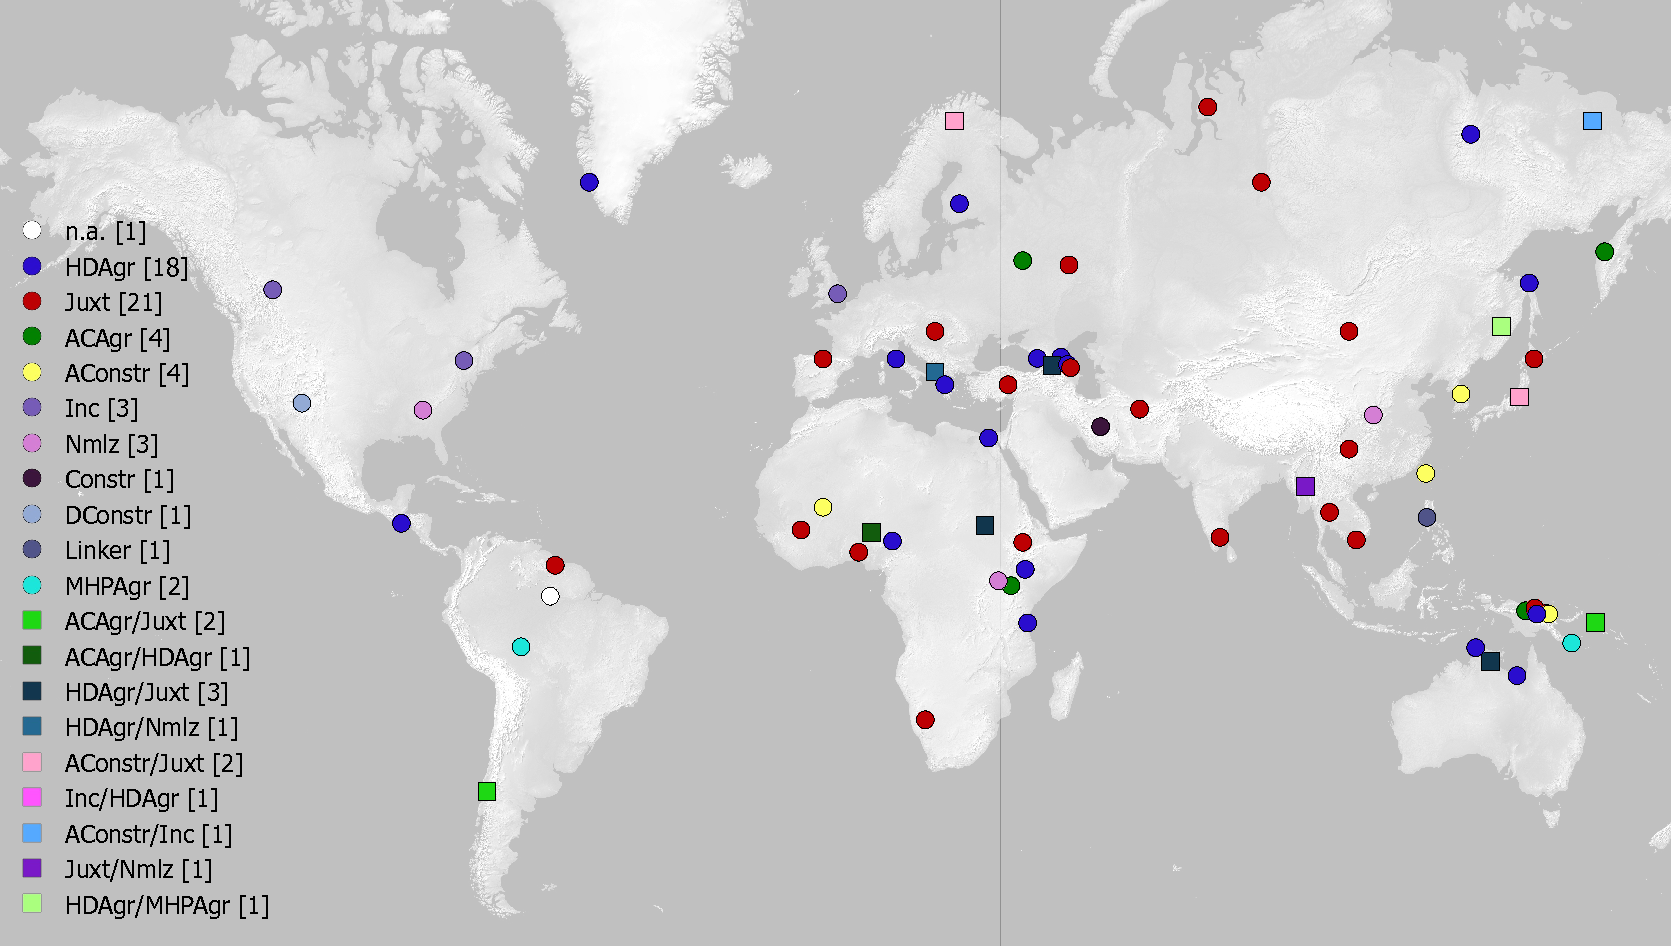
\includegraphics[width=\textheight,angle=90]{WorldMap.jpg}
\label{WorldMap}
\end{sidewaysfigure}

\newpage
\begin{sidewaysfigure}
    \begin{minipage}[b][8cm][c]{2\baselineskip}
        \caption[Adjective attribution marking, World, main types]{Adjective attribution marking in the world's languages; (unbalanced) sample of 71 languages coded for main morpho-syntactic types}
    \end{minipage}
%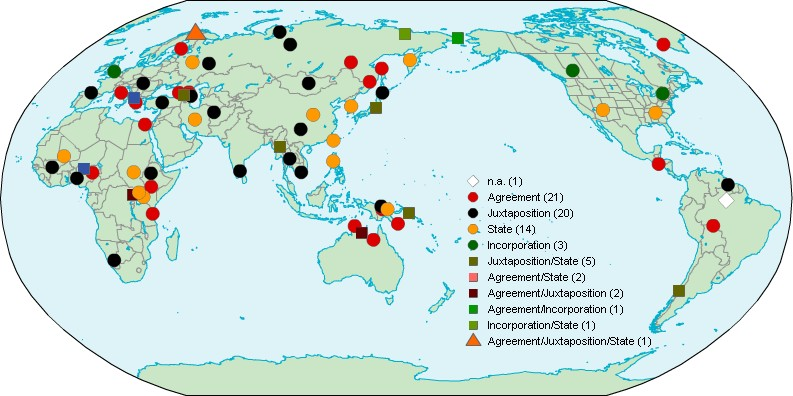
\includegraphics[width=\textheight,angle=90]{WorldMapTyp.jpg}
\label{WorldMapTyp}
\end{sidewaysfigure}

\newpage
\begin{sidewaysfigure}
    \begin{minipage}[b][8cm][c]{2\baselineskip}
        \caption[Adjective attribution marking, North Eurasia]{Adjective attribution marking in the languages of North Eurasia; 85 languages representing all genera of the area}
    \end{minipage}
%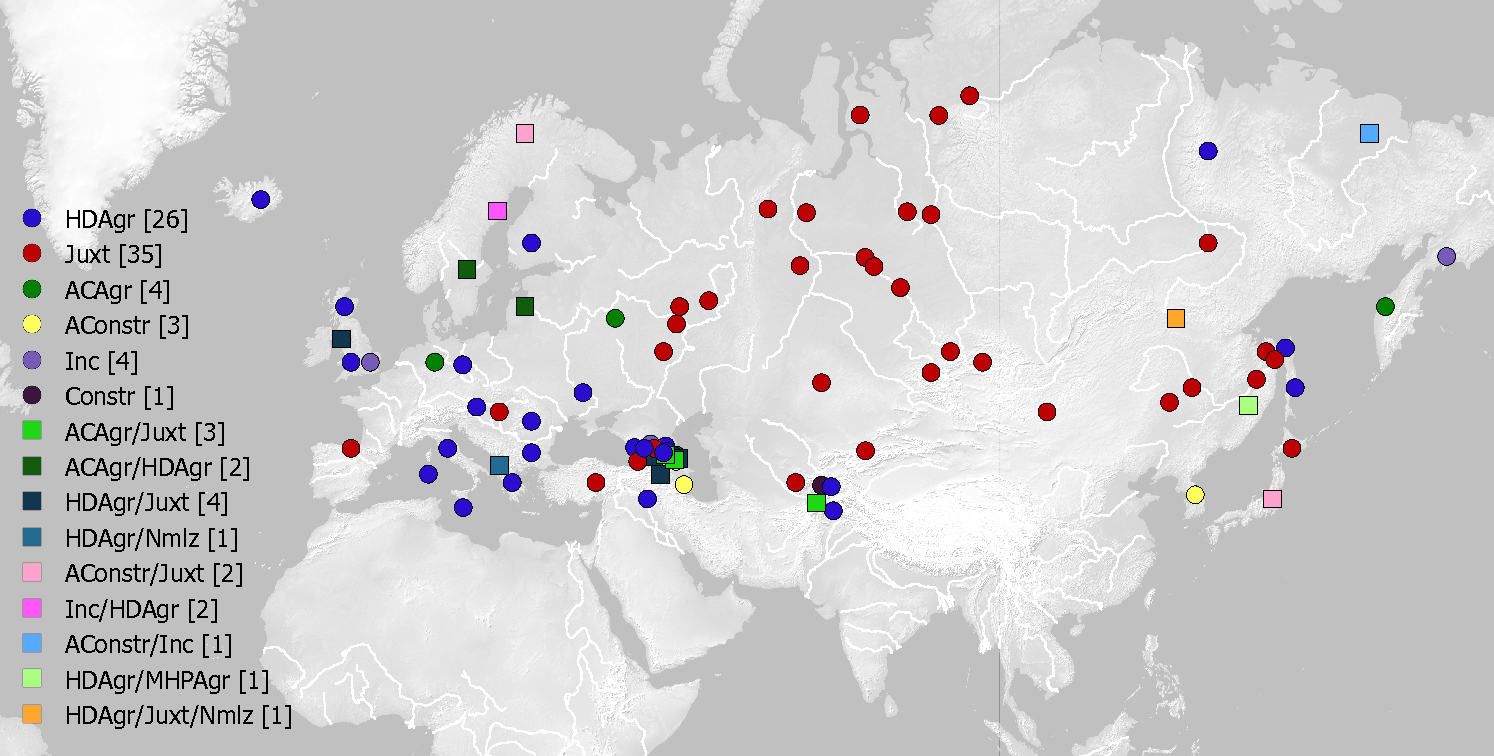
\includegraphics[width=\textheight,angle=90]{NEMap.jpg}
\label{NEMap}
\end{sidewaysfigure}

\newpage
\begin{sidewaysfigure}
    \begin{minipage}[b][8cm][c]{2\baselineskip}
        \caption[Adjective attribution marking, North Eurasia, main types]{Adjective attribution marking in the languages of North Eurasia; 85 languages representing all genera of the area coded for main morpho-syntactic types}
    \end{minipage}
%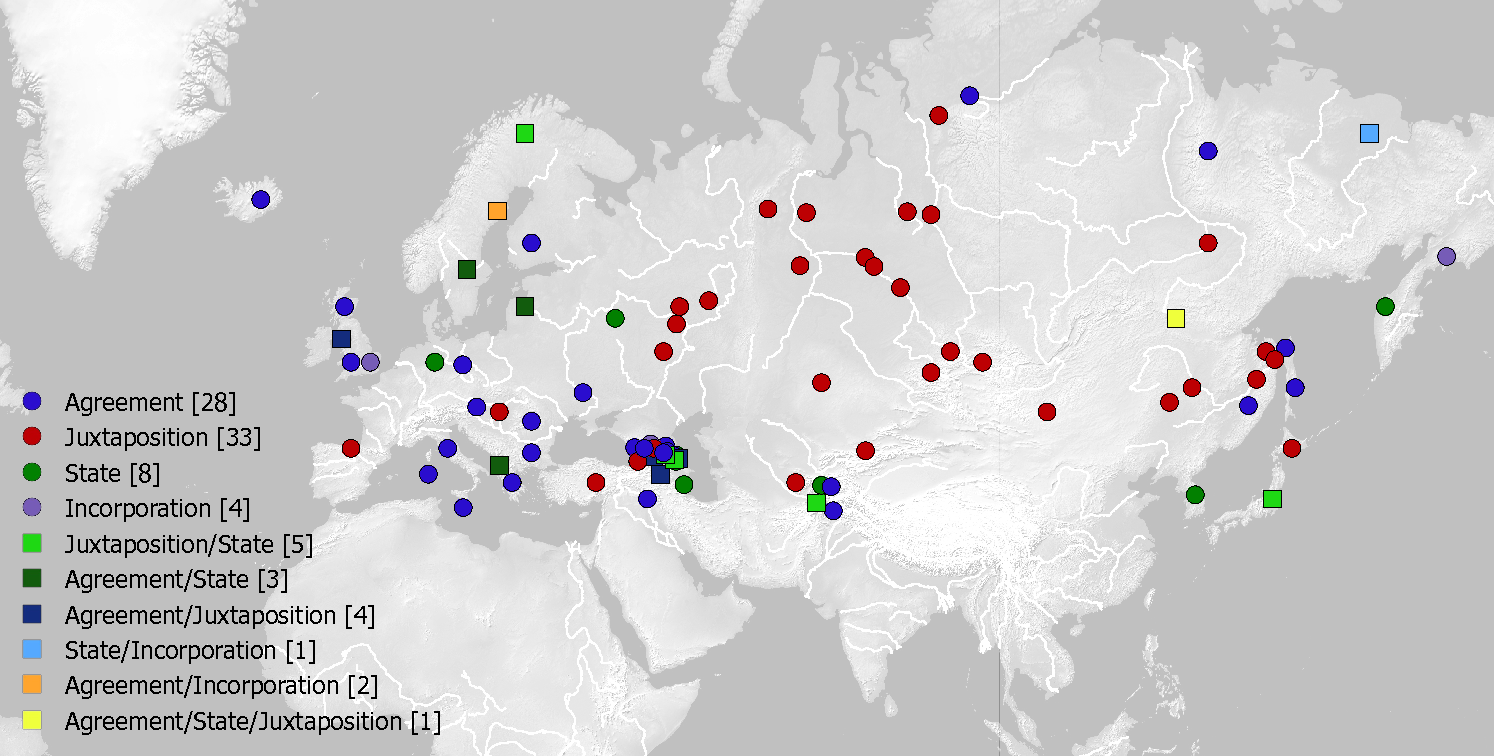
\includegraphics[width=\textheight,angle=90]{NEMapTyp.jpg}
\label{NEMapTyp}
\end{sidewaysfigure}

\newpage
\begin{sidewaysfigure}
    \begin{minipage}[b][8cm][c]{2\baselineskip}
        \caption[Adjective attribution marking, North Asia]{Adjective attribution marking in the languages of \isi{North Asia}; 53 languages}
    \end{minipage}
%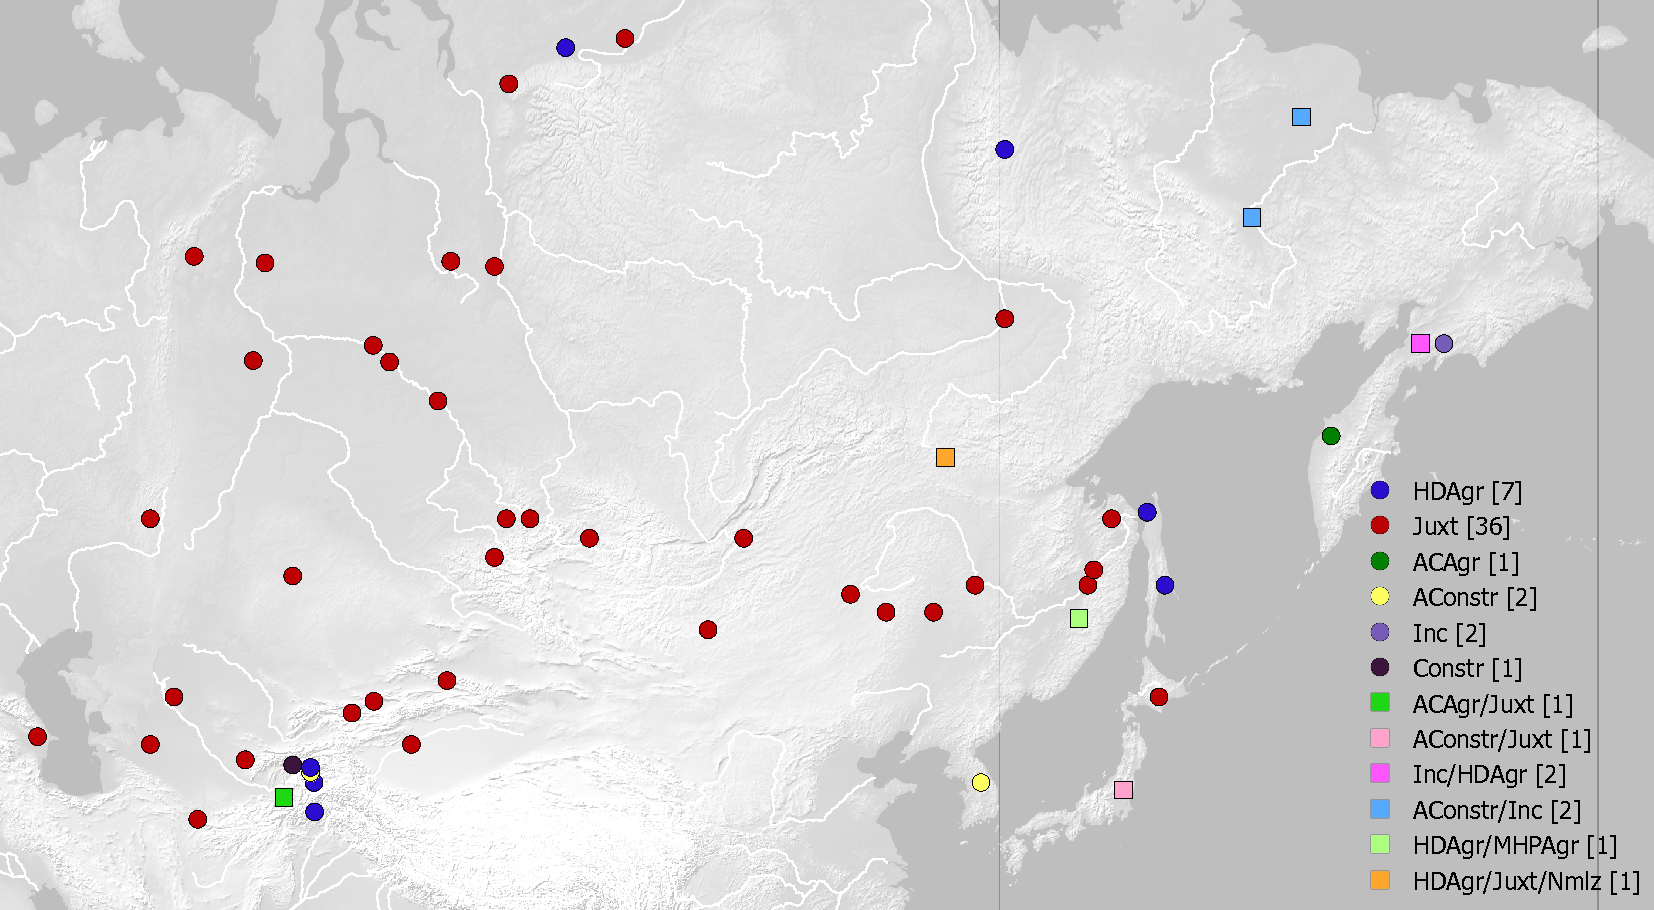
\includegraphics[width=\textheight,angle=90]{NAMap.jpg}
\label{NAMap}
\end{sidewaysfigure}

\newpage
\begin{sidewaysfigure}
    \begin{minipage}[b][8cm][c]{2\baselineskip}
        \caption[Adjective attribution marking, North Asia, main types]{Adjective attribution marking in the languages of \isi{North Asia}; 53 languages coded for main morpho-syntactic types}
    \end{minipage}
%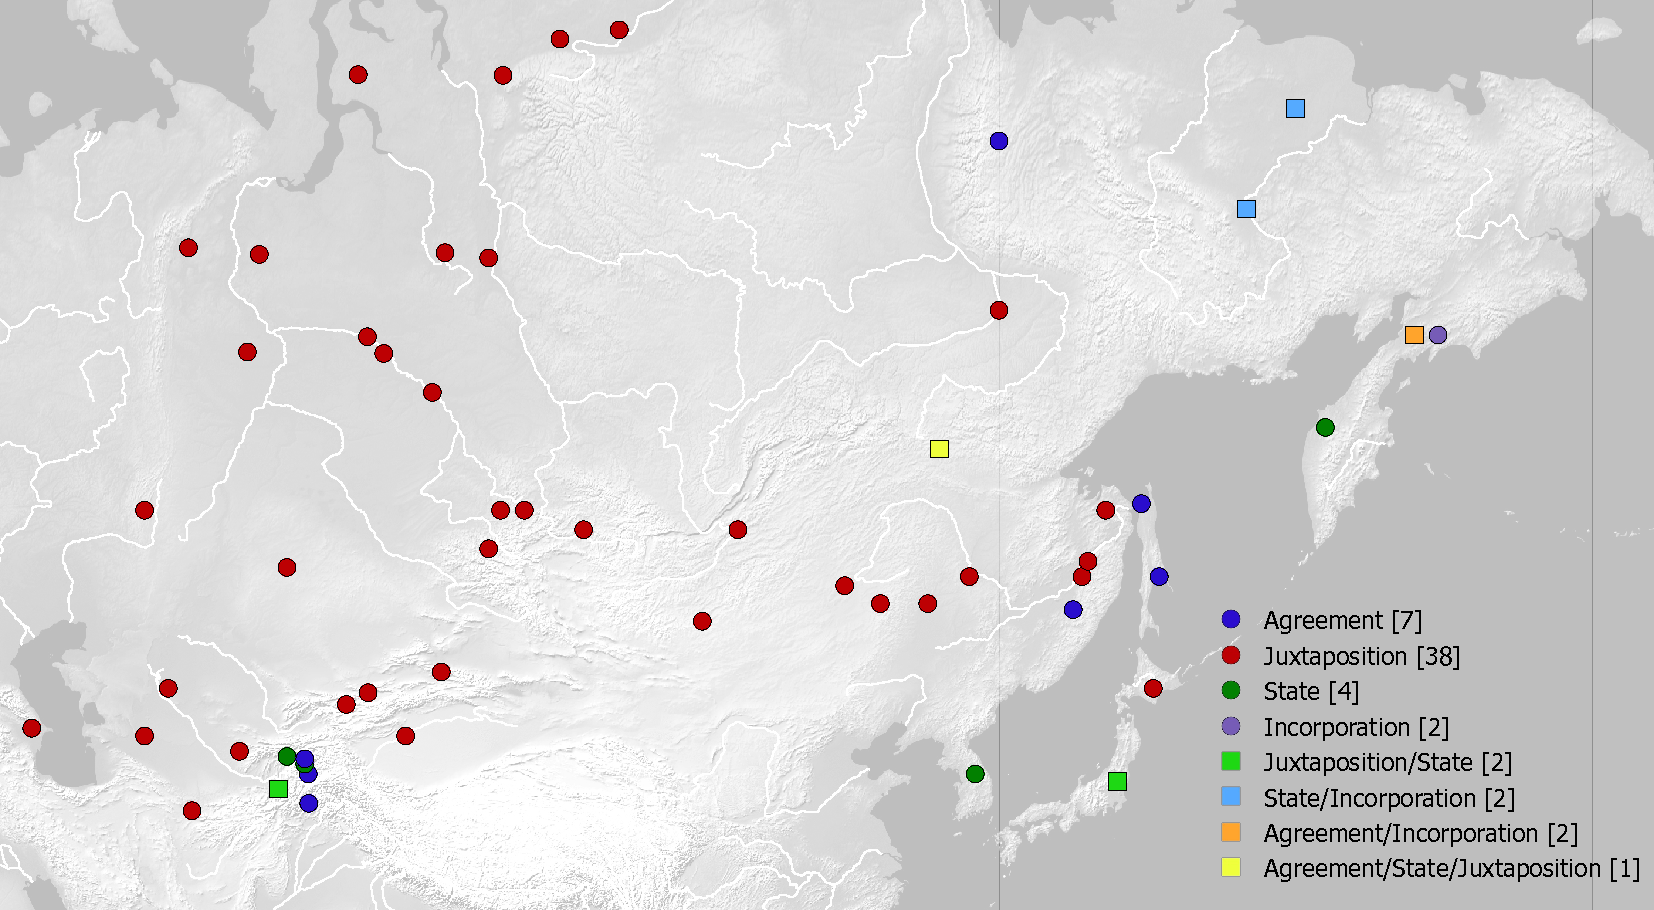
\includegraphics[width=\textheight,angle=90]{NAMapTyp.jpg}
\label{NAMapTyp}
\end{sidewaysfigure}

\newpage
\begin{sidewaysfigure}
    \begin{minipage}[b][8cm][c]{2\baselineskip}
        \caption[Adjective attribution marking, Europe]{Adjective attribution marking in the languages of \isi{Europe}; 123 languages}
    \end{minipage}
%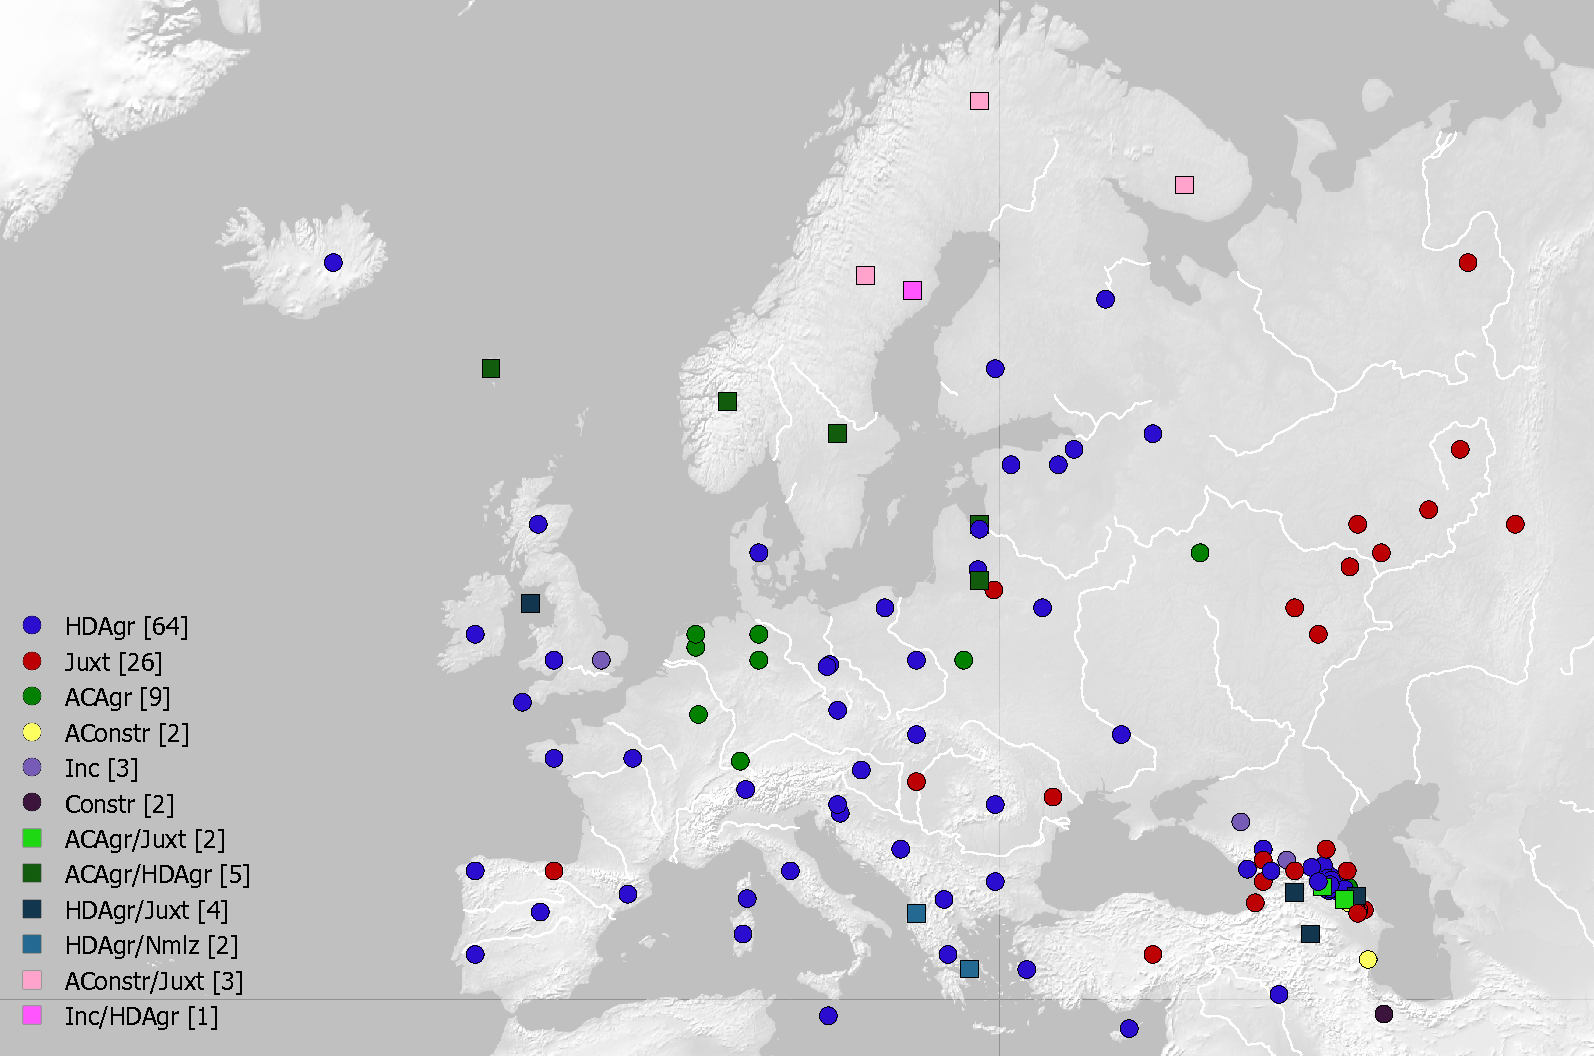
\includegraphics[width=\textheight,angle=90]{EUMap.jpg}
\label{EUMap}
\end{sidewaysfigure}

\newpage
\begin{sidewaysfigure}
    \begin{minipage}[b][8cm][c]{2\baselineskip}
        \caption[Adjective attribution marking, Europe, main types]{Adjective attribution marking in the languages of \isi{Europe}; 123 languages coded for main morpho-syntactic types}
    \end{minipage}
%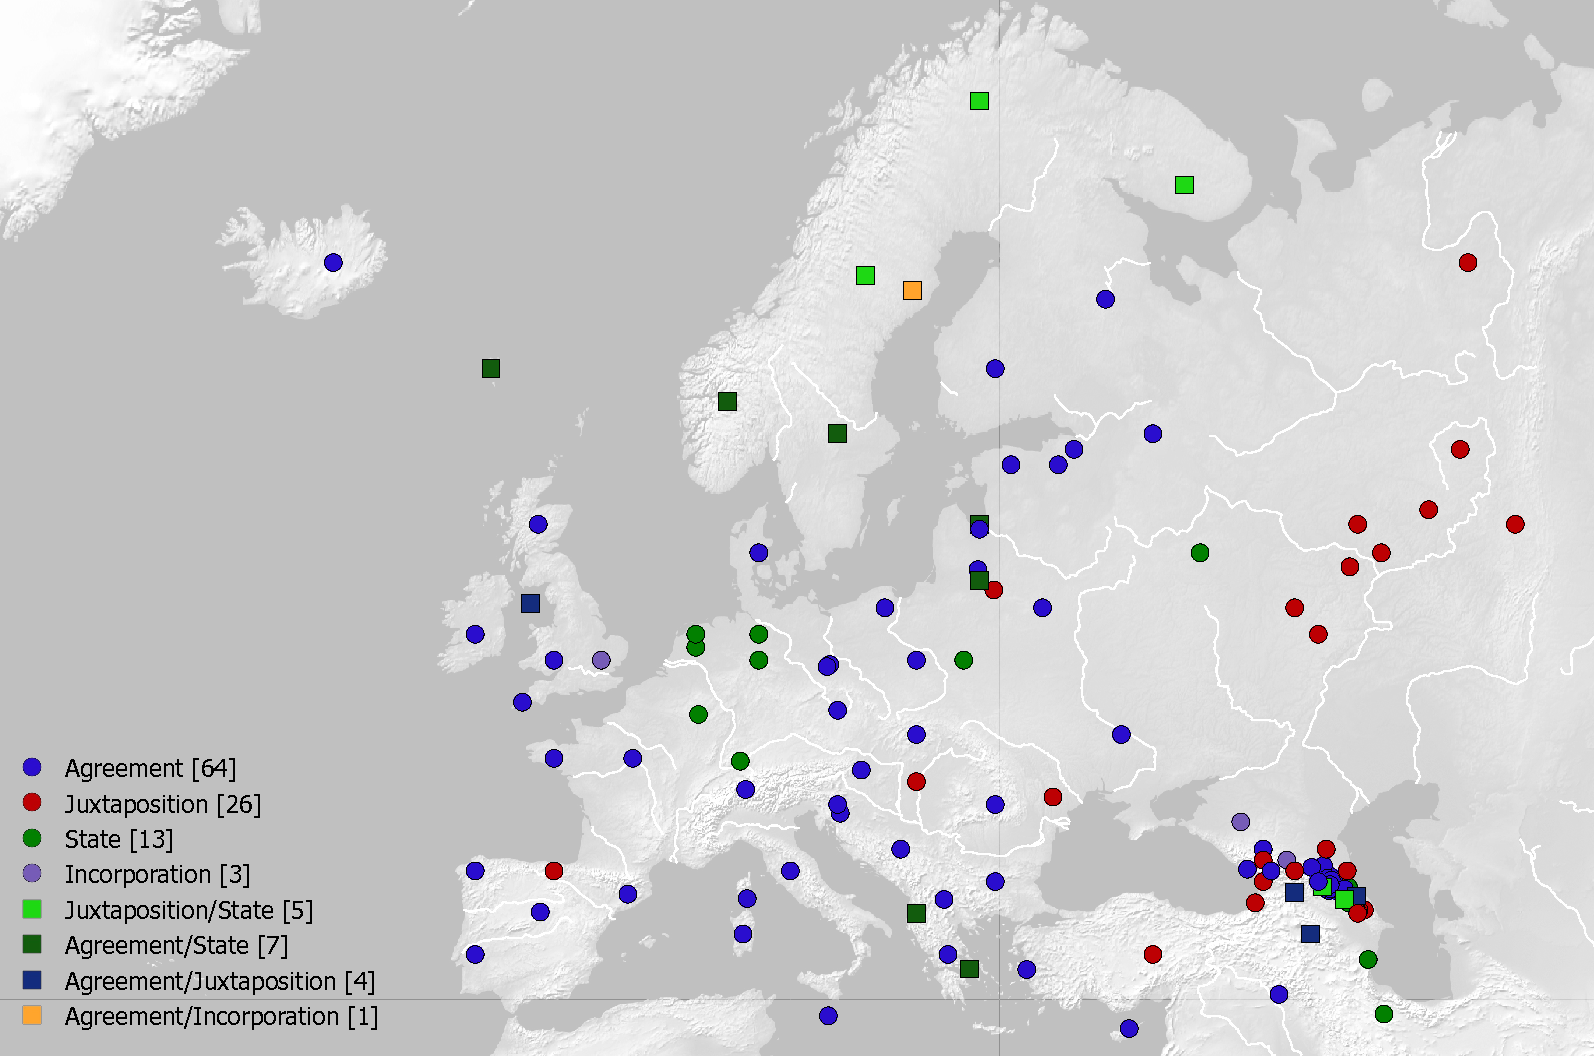
\includegraphics[width=\textheight,angle=90]{EUMapTyp.jpg}
\label{EUMapTyp}
\end{sidewaysfigure}

%completed, except maps
\clearpage

{\sloppy
\phantomsection%this allows hyperlink in ToC to work 
\printbibliography[heading=references] 
\clearpage
   
\addcontentsline{toc}{chapter}{Index} 

\phantomsection%this allows hyperlink in ToC to work
\addcontentsline{toc}{section}{Name index}
\ohead{Name index} 
\printindex
  
\phantomsection%this allows hyperlink in ToC to work
\addcontentsline{toc}{section}{Language index} 
\ohead{Language index} 
\printindex[lan]
  
\phantomsection%this allows hyperlink in ToC to work
\addcontentsline{toc}{section}{Subject index}%started, not completed
\ohead{Subject index} 
\printindex[sbj]
}
\end{document} 
